\documentclass[11pt,letterpaper]{article}
\usepackage[margin=1in]{geometry}
\usepackage{amsmath,amssymb,amsthm,booktabs,array,enumitem,graphicx}
\usepackage[T1]{fontenc}
\usepackage{lmodern,microtype,xurl,hyperref}
\hypersetup{colorlinks=true,linkcolor=blue,citecolor=blue,urlcolor=blue}
\setlength{\emergencystretch}{3em}
\newtheorem{theorem}{Theorem}[section]
\newtheorem{lemma}[theorem]{Lemma}
\newtheorem{proposition}[theorem]{Proposition}
\newtheorem{corollary}[theorem]{Corollary}
\theoremstyle{definition}
\newtheorem{definition}[theorem]{Definition}
\theoremstyle{remark}
\newtheorem{remark}[theorem]{Remark}
\newcommand{\F}{\mathbb F}
\newcommand{\RS}{\operatorname{RS}}
\newcommand{\dist}{\operatorname{dist}}
\newcommand{\List}{\operatorname{List}}
\title{Counterexamples to List and Line Decodability Bounds\\over Prime Fields}
\author{Justin Thaler}
\date{Working draft --- September 17, 2026}
\begin{document}
\maketitle
\begin{abstract}
We give counterexamples to proposed list-decoding and proximity-gap
bounds for Reed--Solomon codes over prime fields. The main line-level
phenomenon is simple: even strictly below the characteristic-based
Elias radius, two far words can have every other affine combination
close to the code.

At every fixed rational rate $\rho\in(0,1)$, write
$\theta=1-\rho-\eta$ for the tested radius. We construct two words at
distance $\theta+(1/2-o(1))\eta$ whose other $p-2$ affine combinations
all have distance exactly $\theta$. The underlying construction also
gives a line nearby at all $p-1$ nonzero parameters, while zero has
distance $1-\rho-1/n$, only one coordinate short of the maximum
possible distance. Here $n=\Theta_\rho(\log p\log\log p)$ and
$\eta\sim H_2(\rho)/\log_2p$. The actual nearby fraction tends to one
while the proposed numerical fraction tends to zero. The nearby
polynomials change with the parameter: their decoding lists are
pairwise disjoint. The same geometry gives failures for batches
consisting entirely of far inputs, including multilinear mixtures.

Decoding ambiguity is unnecessary. Separate constructions have
exponentially more nearby parameters than prescribed, each with a
unique witness. Almost full-gap separation persists after doubling
the proposed exponent constant. We give efficient witness recovery
over sufficiently large splitting primes, and logarithmic-length
existence without that recovery guarantee. A different construction
gives complete nonzero coverage against arbitrary fixed numerical
constants.

Fixing the rate and gap does not bound list size independently of
length: full-length prime-field codes have $n/2$ list elements at
rate $1/4$ and gap $1/8$, still strictly below Elias for large $p$.
Integer-interval domains separately give
$\log L=\Omega_\rho(\eta^{-2}/\log(1/\eta))$, ruling out every uniform
$\exp(O_\rho(1/\eta))$ prescription. Over every sufficiently large
prime, with $b=\log_2p$, we obtain
$\log_2L\ge(1/2-o(1))b^2/\log_2b$ below Elias. We also give fixed-gap
counterexamples to proposed numerical line coefficients. Separately,
at gap $1/n$, codes with global maximum list size exactly $n-k-1$
have $\binom n{k+1}$ uniquely nearby points on one line, attaining
a general puncturing bound.

At a fixed positive gap, we also prove that quadratic growth in the
number of nearby line parameters can be unavoidable without ordinary
correlated agreement. This result has exact rate $1/8$ and gap $1/16$
over $\F_{p^2}$ with growing prime $p$. Superlinear
growth at a fixed positive gap over prime fields themselves remains open.

We apply these results and finite circle-code constructions to the
quantitative premises in the S-two whitepaper. The shrinking-gap
and fixed-gap quantifiers, numerical prescriptions and actual-list-size
statements, and coding premises and complete-protocol conclusions
are distinguished throughout.
\end{abstract}

\section{Introduction}

Many hash-based SNARKs ask the prover to commit to evaluations of
low-degree polynomials. The verifier then checks a small number of
positions and random linear combinations of the committed words.
Analyzing these checks requires quantitative information about the
underlying code. How many low-degree polynomials can be close to one
word? How many points on an affine line can be close to the code?
When do the nearby polynomials imply a common agreement set for the
original words?

These are coding-theoretic questions, but the numerical answers enter
soundness calculations. A bound that is polynomial in the block length
may be adequate for an asymptotic theorem and inadequate for a claimed
concrete security level. Likewise, a bound proved for random evaluation
domains does not automatically apply to a prescribed subgroup. The
field size, domain, and order of quantifiers must be explicit.

This paper gives counterexamples to quantitative list and line bounds
over prime fields. The main results are independent of any particular
proof system. We first prove the general statements, then give finite
circle-code examples and apply them to the two conjectures underlying
the S-two security analysis.

A useful starting point is the root bound. A nonzero polynomial of
degree less than $k$ has fewer than $k$ roots, so two distinct
Reed--Solomon codewords cannot agree in $k$ positions. This proves a
minimum-distance guarantee. It does not answer the first question
above: many polynomials may each agree with an arbitrary received word
in more than $k$ positions, using different agreement sets.

Write $n$ for the number of evaluation points and $\rho=k/n$ for the
rate. We consider agreement on at least $(\rho+\eta)n$ positions,
equivalently relative distance at most $1-\rho-\eta$. The gap
$\eta>0$ is the excess agreement over the rate. Throughout the paper,
we distinguish the largest list at one received word, the number of
nearby parameters on an affine line, and correlated agreement across
that line. None of these quantities can be substituted for another
without a theorem relating them.

The main quantitative message is that the proposed dependence on
$\eta$ fails even when $n=o(p)$. At any fixed rational rate, the proposed
list bound has $\log L=O_\rho(1/\eta)$, whereas our short-domain examples
require
\[
 \log L=\Omega_\rho\!\left(
   \frac{1}{\eta^2\log(1/\eta)}\right).
\]
Thus the exponent must grow almost quadratically in the reciprocal
gap, rather than linearly. The examples remain strictly below the
characteristic-based Elias radius.

The clearest line-level message is that \emph{even below Elias,
two far words can have every affine combination other than the two
endpoints close to the code}. Corollary~\ref{pd:two-far-inputs} places
both endpoints almost half a gap outside the tested radius, while a
random mixture is nearby with probability $1-2/p$. More generally,
for any fixed batch size $t$, all $t$ inputs can lie almost
$(1-1/t)\eta$ outside the radius while a random affine combination
is nearby with probability $1-O(t/p)$. The same obstruction holds
for unrestricted linear combinations and for multilinear mixtures
(Corollary~\ref{pd:far-batching}).

\begin{figure}[tb]
\centering
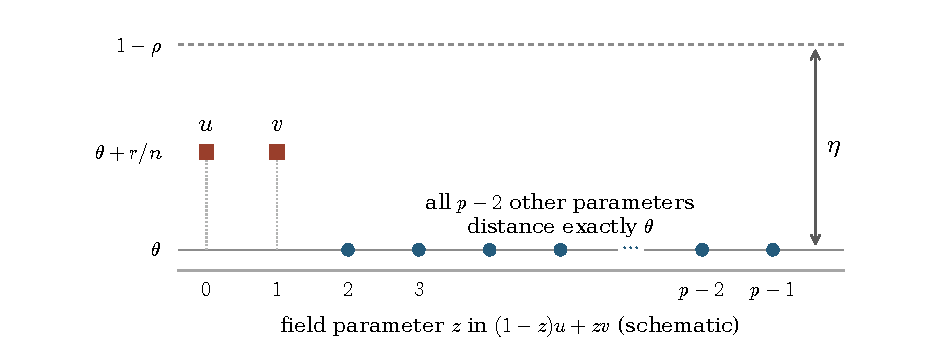
\includegraphics[width=\linewidth]{figures/two_far_inputs.pdf}
\caption{Two far inputs, but all $p-2$ other affine combinations are
nearby (Corollary~\ref{pd:two-far-inputs}). The endpoint separation
$r/n$ approaches half the capacity gap $\eta=(2r+1)/n$. The diagram
suppresses most field parameters.}
\label{fig:two-far-inputs}
\end{figure}

The underlying construction gives an even sharper exceptional point:
\emph{a line can be close to the code everywhere except at one point,
and that point can be only one coordinate short of being maximally far}. At every fixed rational
rate, Corollary~\ref{pd:full-gap} gives prime-field codes for which
all $p-1$ nonzero parameters are nearby, but parameter zero has distance
$1-\rho-1/n$. Every word is within $1-\rho$ of a Reed--Solomon code,
so this is almost the largest distance possible. Its separation from
the tested radius is $(1-o(1))\eta$, almost the entire capacity gap.
The radius remains strictly below Elias. Every nonzero point has
exactly the tested distance, and no codeword is nearby at two distinct
nonzero parameters. The line changes only $2r$ coordinates to improve
the distance by exactly $2r/n$, attaining the Hamming-distance bound.
No pair of codewords explains the line on the required common coordinate set.

The obstruction is that the nearby polynomial changes with the mixing
coefficient. In these complete-coverage examples, no polynomial is close
at two distinct nearby parameters. A root bound controls agreements
between fixed polynomials; it does not force the polynomials selected
at different line parameters to fit together. The construction realizes
this behavior through products of locator values on the evaluation
domain, without any proper subfield.

The $c_1=c_2=1$ numerical prescription predicts a nearby fraction
tending to zero; the actual fraction is $1-1/p$. Thus testing a random
linear combination can find a nearby word with probability arbitrarily
close to one despite an almost maximally far input. Theorem~\ref{cw:punctured-line}
separately defeats any fixed constants $c_1,c_2$, with a fixed positive
separation fraction depending on $c_2$.

Decoding ambiguity is unnecessary for numerical failure. Separately,
Theorem~\ref{pd:deterministic} gives explicit powers-of-two domains where
every nearby point has a unique codeword, recoverable in polynomial time
in $\log p$, and the number of nearby parameters exceeds the numerical
prescription exponentially. The exceptional point is again one coordinate
short of maximum distance. At half rate these examples can have only two
distance levels: every parameter outside the nearby bank is at the far
level, including both displayed endpoints. Thus the obstruction persists
even when proximity along the line
is easy to decide and every accepted parameter has an unambiguous witness.
Corollary~\ref{ou:asymptotic} strengthens this conclusion: for every
fixed $\varepsilon>0$, suitable infinitely many prime fields admit
unique-witness examples whose far point lies at least $(1-\varepsilon)\eta$
outside the nearby radius. These examples use scaled prime-order orbits
and retain efficient witness recovery. They have a sparse nearby set;
they are separate from the complete-coverage construction.
Theorem~\ref{ou:random} obtains the same relative separation and
uniqueness on domains of length $\Theta(\log p)$ by random sampling,
with a polynomial-in-$p$ violation of the numerical bound, but without
a witness-recovery guarantee.
Theorem~\ref{tou:theorem} goes further: two padding orbits preserve
uniqueness and almost full-gap separation even when the proposed
exponent constant is doubled to $c_2=2$. It provides efficient witness
recovery over sufficiently large splitting primes.
Corollary~\ref{tou:short} obtains the same numerical strengthening at
length $\Theta(\log p)$ without that recovery guarantee; its finite
half-rate certificates include separation $38\eta/39$ and a violation
factor greater than $2^9$ over $\F_{2^{44497}-1}$.
A dimension tradeoff preserves uniqueness for every fixed $c_2<3$,
with separation greater than two thirds of the gap
(Corollary~\ref{tou:degree-tradeoff}).

In the full-coverage examples the gap shrinks as $\Theta(1/\log p)$,
and the strongest relative separation approaches the Elias boundary. These results do not
establish superlinear growth in $n$ at one fixed positive gap on short
prime-field domains; that stronger question remains open. Separate
interval-padding constructions give explicit density/separation
tradeoffs and can make the number of missing coordinates grow.

In the fixed-gap line examples, every nearby word can have a unique
nearby codeword. Thus their many nearby parameters do not arise from
decoding ambiguity at individual points of the line. This uniqueness
is a statement about the displayed line, not about all received words
for the code.

A separate construction keeps the code's global maximum list size linear
in $n$, yet has exponentially many uniquely nearby points on a line;
every other point on that line is as far from the code as any word can be
(Theorem~\ref{al:separation}).

\subsection{The list-size obstruction}

Our first result concerns a particularly simple evaluation domain:
$0,1,\ldots,n-1$ in a prime field.

\begin{theorem}[Exponential lists on integer intervals, informal]
\label{thm:informal}
Fix any rational rate $0<\rho<1$. For arbitrarily large $n$, there is a
prime $p$, a rate-$\rho$ Reed--Solomon code over $\F_p$, and a received
word with $2^{\Omega_\rho(n)}$ nearby codewords, where
\[
 \eta=\Theta_\rho\!\left(\frac{1}{\sqrt{n\log n}}\right),
 \qquad \log_2p=\Theta_\rho(\sqrt{n\log n}).
\]
Every listed codeword agrees with the received word on exactly
$(\rho+\eta)n$ positions. The associated distance is strictly below
the characteristic-based Elias radius.
\end{theorem}

The field is large, but its logarithm is sublinear in the block length.
The list is much larger than any bound of the form
$c_1 2^{c_2 H_2(\rho)/\eta}$ with constants depending only on the rate:
the logarithm of that proposed bound is $O_\rho(\sqrt{n\log n})$,
whereas the logarithm of our list size is $\Omega_\rho(n)$.
Here $H_2$ is binary entropy. For a fixed rate it is simply a positive
constant.

The qualification about the field and domain matters. This is a
statement about what can be guaranteed for \emph{every} prime-field
Reed--Solomon code. It does not give exponential lists at a fixed
positive gap, or when the prime is required to be polynomial in $n$.

\paragraph{Finite and uniform refinements.}
The moment count also gives explicit certificates. At length $64$ and
dimension $32$, the exact enumeration in
Section~\ref{sec:overnight-exact64} proves a list of
$5{,}552{,}914{,}238{,}035$ codewords with $34$ agreements.
Over the M31 prime, a further interval example at length $157$ and
dimension $63$ has at least $28{,}169{,}451{,}256{,}663{,}519{,}418$
codewords with $68$ agreements, exceeding the finite prescription with
$c_1=c_2=1$ by more than $2^{34.09967}$
(Section~\ref{sec:overnight-weights}). Proposition~\ref{prop:moment-concentration} gives
an analytic refinement: for each fixed number $m$ of canceled
coefficients and fixed limiting rate, concentration improves the
full-range counting guarantee by a factor of order $n^{m/2}$.
Classical Gram orthogonalization gives explicit constants;
Proposition~\ref{prop:gram-ellipsoid} strengthens the finite bound,
and Section~\ref{sec:gram-gaussian} obtains the Gaussian central-density
constant when $m$ is fixed. These refinements retain the exponent above.
The exact checks certify the finite arithmetic; the proofs establish
the asymptotic statements.

The same construction has a stronger formulation in terms of the gap.
Corollary~\ref{gm:gap-field} rules out every uniform bound whose logarithm
is $o_\rho(\eta^{-2}/\log(1/\eta))$. Moreover, over every sufficiently
large prime field, with $b=\log_2p$, it gives a below-Elias list with
\[
 \log_2 L\ge(1/2-o(1))b^2/\log_2b.
\]
Here $n=(H_2(\rho)^{-1}+o(1))b^2/\log_2b$ and
$\eta=(H_2(\rho)+o(1))/b$. These sharper parameter statements follow
by optimizing the length in the existing moment construction.

\subsection{Why the construction works}

There is a useful way to reverse the usual root-counting argument.
Choose a set $A$ of $r=k+s$ evaluation points, and form its root
polynomial
\[
 F_A(X)=\prod_{a\in A}(X-a).
\]
Suppose many choices of $A$ give the same coefficients in degrees
$r,r-1,\ldots,k$. Let $W$ be this common high-degree part. Then
$G_A=W-F_A$ has degree less than $k$, and it agrees with $W$ at every
point of $A$. Thus each such set produces a member of one decoding
list. The problem has become a counting question about leading
coefficients.

Those coefficients are determined by the first $s$ power sums of $A$.
When $A\subseteq\{0,\ldots,n-1\}$, each power sum is a relatively
small \emph{integer}. There are $\binom nr$ possible sets, but far
fewer possible vectors of $s$ power sums. Some vector must occur many
times. The crucial point is that we count these vectors over the
integers \emph{before choosing the prime}. The count therefore does
not grow with the field size.

For a small example, take
\[
 A=\{0,1,6,7\},\qquad B=\{0,2,5,7\}.
\]
Both sets have size four and sum fourteen. Their root polynomials
therefore begin with $X^4-14X^3$. Subtracting either polynomial from
$W=X^4-14X^3$ leaves a polynomial of degree at most two. Over any prime
larger than seven, on the domain $\{0,\ldots,7\}$ each agrees with $W$
at four positions. The general construction repeats this idea with
many more sets and more moments. This example illustrates the
mechanism; its two codewords are not the quantitative lower bound of
Theorem~\ref{thm:informal}.

\subsection{Lines of received words}

Proof systems often test a random linear combination of several words.
This leads to a related question. Suppose many words on an affine line
$f_z=f_0+zf_1$ are close to the code. Must the nearby codewords fit
together into a single affine line of codewords? Must $f_0$ and $f_1$
agree with two codewords on a large common set of coordinates?

We give three constructions, because these questions have different
quantifiers.

\paragraph{Many nearby points without correlated agreement.}
Corollary~\ref{pd:full-gap} gives complete nonzero coverage with an
almost maximally far exception. On a paired core, even locator
polynomials leave codeword candidates after their common leading term
cancels. A padding block supplies several pairs of new agreements at
once. Multiplicative-character estimates show that the candidates'
joint evaluation images fill almost all possible vectors, so random
padding directions cover every nonzero line parameter.

Theorem~\ref{cw:punctured-line} gives complete coverage against
arbitrary fixed numerical constants. Matching three times as many
moments permits a cubic change of the seed domain without losing the
required common locator prefix. A geometric irreducibility argument
and a finite-field point-count estimate then control outside collisions.

The interval constructions also give elementary alternatives with
quantified nearby density. Division by $X-\tau$ yields
$\Omega(p/\log p)$ nearby labels at logarithmic length
(Theorem~\ref{thm:logarithmic-lines}); padding gives the stronger density
bounds in Theorems~\ref{fg:dense-lines} and~\ref{fg:near-unit-density}.
Corollary~\ref{fg:slow-separation} makes the number of coordinates outside
the radius grow while retaining density tending to one. These variants
use padded interval domains. The complete-coverage constructions use
random paired domains or cubic images of intervals with added coordinates.

\paragraph{An obstruction that persists at a fixed gap.}
The gap in Theorem~\ref{thm:informal} shrinks with $n$. To address
asymptotic claims at a fixed gap, we start with one fixed large list
and replace each evaluation point by $B$ points on which $X^B$ has
the same value. Polynomial composition preserves the rate, relative
agreement, and list size. Suitable prime fields exist for every $B$.

An anchored version removes one common agreement point and divides by
its linear factor. Padding then produces many nearby challenges while
keeping every common coefficient agreement below the threshold.
Theorem~\ref{fg:anchored-fixed-gap} gives actual failure of correlated
agreement at a fixed rate and gap, with a linear count whose coefficient
has logarithm of order $\eta^{-2}/\log(1/\eta)$.
Every nearby word on these lines has exactly one nearby codeword,
while the parameter-zero word is one coordinate beyond the radius.
The obstruction persists without local list ambiguity.
The same exceptional-count lower bound also has realizations with
$p=n^{O_{\rho,\eta}(1)}$ (Corollary~\ref{fg:polynomial-fields});
uniqueness is not asserted for those smaller-field realizations.
No remainder that is $o(n)$ along this family can absorb a smaller
linear coefficient. The simpler selection argument in
Theorem~\ref{fg:fixed-gap} is retained as a preliminary construction.

\paragraph{Small lists with many isolated nearby line points.}
Large lists are not the only obstruction. At every fixed rate $\rho=k/n$,
we also construct codes whose maximum list size is exactly $n-k-1$,
together with a line having $\binom n{k+1}$ nearby parameters. Each
nearby word has a unique nearby codeword, yet no parametrized codeword
line contains more than $n-k$ of those witnesses. The gap is $1/n$.
At rate one-half these bounds are $n/2-1$, $\binom n{n/2+1}$, and $n/2$,
respectively. The construction combines
an elementary line spanned by consecutive powers with a domain chosen
using a known list-decoding theorem for random Reed--Solomon codes.
Proposition~\ref{prop:puncturing-bound} shows that its nearby-parameter
count is optimal among lines without correlated agreement at this radius.

\paragraph{What remains open at a fixed positive gap.}
Our fixed-gap lower bound forces a large coefficient of $n$, but does
not force a superlinear exponent. Proposition~\ref{prop:exact-list-amplification}
identifies a sufficient route: a source list of size $L$ at length $N$
gives $\Omega(\min\{NL,p\})$ full-support MCA exceptions over the same
prime field, after exactly halving both rate and gap. Thus lists of size
$N^c$ over superpolynomial prime fields would force exceptions of order
$N^{c+1}$. The missing ingredient is a growing fixed-gap list on domains short
enough relative to the prime; full-length lists with $N=p-1$ cannot give superlinear scalar-label counts.
The factor-of-two parameter change is not essential:
Corollary~\ref{cor:sparse-list-amplification} uses a small positive
padding fraction to preserve any strict margin above a continuous
sufficient agreement curve. Thus the same exponent transfer can stay
inside an open regime where a sharper upper bound is available.

\paragraph{Sharp algebraic counts need not give sharp proximity gaps.}
For a differential equation of fixed order $d$, fixed jet degree, and
fixed challenge degree, Appendix~\ref{app:isolated-sharpness} proves
that the actual regular polynomial--challenge locus has at most
$O(D^{d+1})$ isolated points for message degree $D$. An explicit
Wronskian family attains $\binom{D+d+1}{d+1}$ such points, all regular,
with distinct labels over suitable prime fields. Nevertheless, that
family has only constantly many nearby labels on any received line
at a fixed positive agreement gap. At every fixed order $d$, Appendix~\ref{app:higher-positive-components}
also bounds the degree of each positive-dimensional actual stratum
by $O(D^d)$, and gives examples attaining this exponent. The first-order
case in Appendix~\ref{app:actual-first-order} is linear in $D$.
These results distinguish sharpness of algebraic candidate counts
from the still-open fixed-gap superlinear proximity-gap lower bound
over sufficiently large prime fields.
Proposition~\ref{prop:rational-envelope} extends this obstruction to
arbitrary candidate families with bounded-degree rational residuals
after a common normalization: their full-support exceptional count
is linear, regardless of how many algebraic candidates they contain.
Theorem~\ref{thm:nonsingular-agreement-mca} gives a further first-order
restriction: bad labels with a positive fraction of nonsingular
agreement coordinates number only $O(n)$ at a fixed positive gap.
For $R(X,z)P'=\mathcal A(X,z,P)$ this bounds all bad labels linearly
when $\deg_XR$ also stays a fixed positive fraction below the
agreement threshold. A nonlinear two-solution family attains $n/2$
bad labels at fixed rate and gap. The general first-order conjecture
still requires controlling singular agreement coordinates.
Appendix~\ref{app:riccati-cross-ratio} removes that restriction for
a fixed nonlinear Riccati equation, proving a linear full-support
bound and a sharp ordinary-list bound with prime-field equality families.
Appendix~\ref{app:triangular-differential} gives a different criterion
for challenge-dependent equations: if the highest coefficient equations
determine all nonconstant message coefficients by a triangular linear
system, bounded challenge and nonlinear degrees imply only $O(n)$ bad
labels at fixed agreement excess. This includes candidates singular at
every agreement coordinate. The criterion applies to a specified
differential equation covering the candidates; it does not construct
such an equation for an arbitrary received line or settle the general
first-order conjecture.
Appendix~\ref{app:singular-cover-riccati} removes both the triangular
pivot restriction and any bound on the derivative coefficient's degree
for bounded-challenge monic Riccati families. Above agreement $5D/3$
with fixed linear slack, these families have only $O(n)$ bad labels,
even when the singular coordinates move with the challenge. This
includes the quarter-rate first-order agreement regime. A separate
construction attains linearly many bad labels with every agreement
coordinate singular, showing that singularity alone does not force
a superlinear exceptional count.

Appendix~\ref{app:hermite-johnson} controls a broader singular mechanism:
dependence of degree at most three on the derivative, with bounded dependence on the
value and the challenge and unrestricted coefficient degrees in $X$.
If the specialized equation does not vanish identically in both the
derivative and the challenge at any domain coordinate, then agreement
$A>\sqrt{Dn/2}$ with fixed normalized slack gives only $O(n)$ bad
full-support labels. The proof uses both the value and derivative at
singular matches, and includes polynomial solutions that appear only
at special challenge values. Thus a large persistent singular set is
not by itself an obstruction in this regime; an uncontrolled set of
coordinates carrying no equation remains a limitation. As with the
preceding results, one common identity must contain the candidates.

For one explicit equation we can describe the obstruction exactly.
Its complete polynomial solution family contains a linear-size list at
agreement $3/8$, but every received word has only
$O(\varepsilon^{-2})$ members of that family at agreement
$3/8+\varepsilon$. A majority construction attains
$\Omega(\varepsilon^{-2})$ for sufficiently large primes
(Theorem~\ref{thm:dickson-sharp-transition}). Thus the growing list in
this family has an exact agreement threshold. This conclusion concerns
the classified solution family, rather than the full Reed--Solomon code.
We also control every degree-two rational first-integral family in
characteristic $p>10D$: at agreement $D+\eta n$, its list size is at most
$\max\{40,\lfloor1/\eta\rfloor\}$
(Theorem~\ref{thm:quadratic-rational-pencil-list}).
This includes denominators depending quadratically on the candidate
value. The proof derives a height bound from five polynomial sections
and applies the classical square-value theorem of Pasten and Wang;
it gives a family-specific list bound, not a general proximity-gap bound.

For weighted monic-cubic first integrals with denominator depending only
on $X$, we prove a corresponding bound of $O(1/\eta)$ at agreement
$D+\eta n$, in characteristic zero or $p>\max\{3,2D\}$
(Theorem~\ref{thm:weighted-cubic-first-integral-list}).  On prime-field
domains this includes every rate below $1/2$.  The proof treats repeated
basepoints and positive-dimensional critical loci: nonconstant Frobenius
critical values force too few distinct denominator roots to support a
large list.  These conclusions concern the specified first-integral
families; a cubic differential equation alone does not suffice.
More generally, every fixed monic value degree has an $O_b(1/\eta)$
list bound when the original critical locus is finite
(Theorem~\ref{thm:general-first-integral-zero-dimensional}). In
characteristic zero, or $p>b(b-1)D$, a larger list forces a constant
fiber with a repeated factor
(Corollary~\ref{cor:general-first-integral-repeated-fiber}). This is a
necessary condition on the first integral, not a classification of the
remaining families.

A separate exact construction gives a quarter-rate Reed--Solomon code
of length $28$ and a received word whose complete nearest-codeword list
has exactly seven members, each agreeing on exactly half the coordinates
(Theorem~\ref{thm:seven-cubic-bank}). It holds over arbitrarily large
prime fields. More generally, a polynomial pullback preserves this exact
list size at length $14m$ and degree bound $3m$ for every $m\geq1$.
The construction follows from two explicit cyclotomic identities;
completeness follows from saturated pairwise root counts and a
seven-point interpolation obstruction. At its underlying cubic parameters,
seven is optimal for every fourteen-point domain in characteristic zero
and in every sufficiently large characteristic
(Theorem~\ref{thm:global-seven-cubics}). This sharp upper bound concerns
the cubic parameters, not arbitrary quarter-rate length-twenty-eight codes.

Another construction verifies two successive one-pole extensions at
quarter rate. Over arbitrarily large prime fields, it gives six distinct
polynomials of degree at most fourteen, each agreeing with one word on
thirty of sixty coordinates (Theorem~\ref{thm:six-word-one-pole}).
The proof uses an exact finite-field witness and two independent
nonsingular lifting certificates. This is a fixed-size construction;
unbounded iteration remains open.

\subsection{Finite examples on circle codes}

We also study a different regime: the fixed prime $p=2^{31}-1$ and
domains on the norm-one circle. These are structured evaluation
domains used by Circle STARKs. At the common parameters
\[
 n=2^{26},\qquad \rho=\frac12,\qquad
 \eta=\frac{33}{1024}-\frac{2}{n},
\]
we obtain the following finite lower bounds:
\begin{center}
\begin{tabular}{lr}
\toprule
Object constructed & Guaranteed size\\
\midrule
One base-field decoding list & $>2^{40}$\\
Distinct nearby parameters on an extension-field line & $>2^{74}$\\
\bottomrule
\end{tabular}
\end{center}
The line has no correlated agreement at the specified threshold.
The constructions give existence with explicit numerical certificates;
they do not enumerate these very large lists.
Section~\ref{sec:circle-overview} explains the idea, and
Appendix~\ref{app:circle} gives the coefficient calculations.

\subsection{Context and organization}

Proximity gaps are established tools in the analysis of low-degree
tests~\cite{bciks,bchks}. In particular, existing theorems give
proximity guarantees in specified radius regimes. Our fixed-rate
asymptotic examples have $\eta\to0$ and eventually lie beyond the
Johnson radius $1-\sqrt\rho$, although they remain below the
characteristic-based Elias radius. The distinction between these
radii is essential when comparing the results with proved soundness
bounds for a low-degree test.

The connection between equal subset moments, elementary symmetric
functions, and Reed--Solomon decoding is established prior work;
Gandikota, Ghazi, and Grigorescu use this connection in decoding
hardness results~\cite{ggg}. The integer moment pigeonhole argument is
also classical: Borwein, Erd\'elyi, and K\'os use derivative vectors of
binary polynomials in the proof of their Theorem~2.7~\cite{bek}.
Restricting that argument to fixed-weight subsets and retaining a large
fiber, followed by the standard locator correspondence, already yields
the asymptotic exponent
$\log L=\Omega_\rho(\eta^{-2}/\log(1/\eta))$ used here.
Our interval counts give sharper finite bounds and an application to the
specific uniform prime-field conjecture; we do not claim a new moment
counting mechanism. The affine-line distance profiles require additional
constructions. The number-theoretic splitting theorem used in the lift is
also classical.

Prime-field list constructions using multiplicative cosets also appear
in work of Guruswami and Rudra, presented in
Rudra's thesis~\cite[Section~6.4.3]{rudra-thesis}. Those full-field
examples already use cancellation of leading coefficients through
unions of multiplicative orbits. Their displayed coset bank has
logarithmic size $O(1/\eta)$; our interval construction gives the
larger, almost-quadratic reciprocal-gap exponent above. Neither
comparison supplies growing lists at one fixed positive gap.

The generic list-profile upper bound is due to Brakensiek, Gopi, and
Makam~\cite{bgm}. At every fixed positive rate, Roth's ordinary
list-decoding bound~\cite{roth} gives the matching lower bound for all
sufficiently large lengths. We include an explicit construction that
also covers the remaining finite parameters $k\ge2$, without claiming
priority for that construction. The separation here combines these
list bounds with a line containing many isolated nearby points.

Brakensiek, Chen, Putterman, Zhang, and Zheng~\cite{bcpzz-capacity}
give polynomial-in-$p$ time list decoding up to capacity for arbitrary
prime-field evaluation sets at fixed rate and fixed slack, subject to
their field-size hypotheses. In particular, their all-rates statement
assumes $p\ge C(R,\delta)n$; their formal Corollary~5.1 gives runtime
and list size $p^{O_{R,\delta}(1)}$. Such polynomial list bounds allow growing lists;
they do not imply the uniform reciprocal-gap list bounds or the
affine-line conclusions considered here.

Goyal, Guruswami, Sun, and Wootters~\cite{ggsw} give further recent
proximity-gap and correlated-agreement bounds for random Reed--Solomon
domains. Their results allow general received curves and retain explicit
slack and field-size hypotheses. They provide useful context for the
shrinking-gap regime studied here, but do not subsume the specific
actual-list-size separation in Theorem~\ref{al:separation}.

Krachun, Kazanin, and Hab\"ock~\cite{kkh} construct large lists and
affine-line obstructions on multiplicative subgroups of prime fields,
with a gap of order $1/\log n$. Our interval construction addresses
a different family of domains and gives lists larger than every fixed
exponential in the reciprocal gap. The paired-domain construction adds
a different line phenomenon: two quantitatively far inputs have all
$p-2$ non-endpoint mixtures nearby, and the underlying distance profile
can have one almost maximally far point and $p-1$ nearby points. These
statements use specially constructed domains and a shrinking gap.
The multiplicative-subgroup domains and polynomial-size alphabets in
their theorem remain separate advantages. Thus the advance claimed here
is the quantitative coverage, separation, and reciprocal-gap dependence;
prime-field counterexamples themselves are already established prior work.
Our finite circle examples concern the evaluation spaces of
Circle STARKs~\cite{circle}.

The Proximity Prize's orbit-pencil upper certificate also uses
multiplicative fibers and a fixed core~\cite{orbit-pencil}. Our circle
construction expresses the analogous core through a common anchor and
division at two circle points. Appendix~\ref{app:common-core} makes this
change of presentation explicit. The contest's field, code, and score
are different from the circle specialization considered here.

The distinction between fixed and shrinking gap separates our
results from the fixed-gap polynomial-in-$n$ list bound stated in the
recent preprint of Jeronimo~\cite{jeronimo}. Our exponential-list
family has a shrinking gap. Our fixed-gap family preserves a fixed finite
list of witnesses as $n$ grows; it does not bound the full decoding list
by that constant. Neither construction contradicts such a polynomial bound.

The current Dao--Kominers--Thaler paper~\cite{dkt2026} gives, above its
first-order curve by margin $\eta_1$, list bound
$O_\rho(n/\eta_1^2)$ and full agreement-set MCA exceptional count
$O_\rho(n^2/\eta_1^4)$ in sufficiently large characteristic. Its capacity
bounds have exponents depending on the fixed capacity gap.
There are two qualitative intrinsic lower bounds:
Proposition~\ref{prop:full-length-fixed-gap} gives $n/2$ list elements
over prime fields at fixed rate $1/4$ and gap $1/8$;
Corollary~\ref{cor:quadratic-extension-fixed-gap} gives
$\Omega(n^2)$ full agreement-set MCA exceptions over quadratic extension
fields of growing prime characteristic, at fixed rate $1/8$ and gap $1/16$.
The latter rules out a universal linear capacity MCA bound in that
larger field class. Theorem~\ref{thm:ordinary-ca-superlinear} also gives
$\Omega(n^2)$ nearby labels with no ordinary
correlated agreement, over quadratic extensions at exact rate $3/13$
and capacity gaps bounded below by $3/26$ (not fixed exactly).
Corollary~\ref{cor:ordinary-ca-fixed-gap} obtains quadratic ordinary-CA
counts at exact rate $1/8$ and gap $1/16$ over $\F_{p^2}$,
with at least $\lceil n^2/192\rceil$ exceptions
(Proposition~\ref{prop:ordinary-ca-field-degree}).
Thus quadratic length dependence is necessary for ordinary
correlated-agreement exceptions in the large-characteristic capacity regime.
In particular, at these parameter pairs no uniform $o(n^2)$
exceptional-count bound holds in this field class.
Corollary~\ref{cor:ordinary-ca-parameter-family} extends the exact
parameters to rate $b/d$ and gap $1/d$ for $b\in\{2,3,4,5\}$ and
$d\ge b+7$, over the fixed-degree extensions $\F_{p^{2^{b-1}}}$,
including rate $2/9$ and gap $1/9$ over $\F_{p^2}$.
These results do not establish first-order-regime tightness or force
an exponent growing as the gap shrinks. Over prime
ambient fields, even a superlinear exceptional-count lower bound at
one fixed positive gap remains open here. The large gap-dependent
coefficient in our linear lower bound must not be confused with a
growing exponent of $n$.
Likewise, optimality of a specified interpolation dimension count is a
statement about that proof method, not an intrinsic list or MCA lower
bound. The capacity gap and the margin above the first-order curve are
different parameters.
A separate support-count audit establishes a restricted form of
method tightness for the current first-order formulas. At rate $1/4$,
every monomial support downward in the value variable, with full
derivative-weighted coefficient prefixes, necessarily incurs inverse-margin
powers two in the squarefree list budget and four in the regular-family
MCA budget, under either current challenge-counting test.
The row-test proof uses a positive-feasibility reduction that deletes,
truncates, and rearranges columns; ordinary sorting alone need not work.
For that test the result also covers total-degree-graded,
translation-stable nonmonomial jet spaces. A separately justified filtered
row test gives the same costs when the maximum jet degree is at most
the code's polynomial degree bound.
The proof uses a corrected finite-length margin and assumes characteristic
zero or characteristic exceeding every retained total jet degree.
It does not cover arbitrary filtered nonmonomial spaces,
multiple equations, or counting actual component degrees.
The proof and precise hypotheses appear in the companion note,
\emph{A Sharp Quarter-Rate Threshold for a First-Derivative
Interpolation Dimension Count}, maintained with this manuscript.


Sections~\ref{sec:lists}--\ref{sec:actual-list} prove the general list
and line results. Section~\ref{sec:circle-overview} gives finite circle
examples. Section~\ref{sec:snark-security} explains what these results
imply for hash-based SNARK analyses, and Section~\ref{sec:stwo}
applies them to S-two. Section~\ref{sec:coding-open-questions} states
the remaining coding-theoretic questions. The first appendices contain
the circle proofs, quotient calculations, and finite certificates.
The later appendices study restrictions on possible constructions:
rational fibers, binary-affine locator families, and polynomial
differential equations. These additional results address the open
fixed-gap problem; the main list and line counterexamples do not
depend on them.

% General coding-theory sections. Uses the shared theorem environments in main.tex.
\section{Large lists from subsets with equal moments}
\label{sec:lists}\label{im:section}

The construction starts with a simple observation: if two polynomials differ
by a polynomial whose roots are a set $A$, then they agree at every point of
$A$. We will choose many sets $A$ whose vanishing polynomials have the same
leading coefficients. Subtracting those common coefficients will give many
low-degree polynomials close to one received word.

\paragraph{Notation.}
For a field $F$ and a set $D\subset F$ of $n$ distinct points, write
\[
 \RS(F,D,k)=\{(P(x))_{x\in D}:\deg P<k\}.
\]
This code has dimension $k$ and rate $\rho=k/n$, provided $k\le n$.
The relative Hamming distance between two words is the fraction of coordinates
on which they differ. A list at radius $\theta$ consists of all codewords
within that distance of a received word. Write $\ell_C(\theta)$ for the largest
such list over all received words. We parameterize the radius by
\[
 \theta=1-\rho-\eta.
\]
Thus a nearby codeword agrees with the received word on at least a
$\rho+\eta$ fraction of the coordinates. We call $\eta>0$ the gap from
$1-\rho$.

All logarithms are base two, and
$H_2(t)=-t\log_2t-(1-t)\log_2(1-t)$ is binary entropy. For characteristic $p$,
define
\[
 H_p(t)=\frac{H_2(t)+t\log_2(p-1)}{\log_2p}.
\]
The characteristic-based Elias radius is the solution of
$H_p(r_E)=1-\rho$ on the increasing branch $[0,1-1/p]$.
We will keep our examples strictly below this radius. The simple estimate
\begin{equation}\label{im:entropy}
 H_p(\theta)\le\theta+\frac1{\log_2p}
\end{equation}
shows that it suffices to have $\eta\log_2p>1$.
In our prime-field examples $p>n$ and $\rho\ge1/n$, so
$0\le\theta<1-1/p$ as required.

\subsection{Why matching moments produces a list}

Consider the $34$-element subsets $A$ of $\{0,\ldots,63\}$. Their vanishing
polynomials begin
\[
 F_A(X)=\prod_{a\in A}(X-a)
 =X^{34}-\Bigl(\sum_{a\in A}a\Bigr)X^{33}
   +\Bigl(\sum_{a<b\in A}ab\Bigr)X^{32}+\cdots.
\]
Subsets with the same sum and the same sum of squares have the same three
leading coefficients, because
\[
 \sum_{a<b\in A}ab
 =\frac{(\sum_{a\in A}a)^2-\sum_{a\in A}a^2}{2}.
\]
Let $W$ be those common leading terms. Each polynomial $W-F_A$ has degree
less than $32$ and agrees with $W$ at exactly the $34$ points of $A$.
Consequently, a large class of subsets sharing these two moments gives a
large list in a rate-one-half Reed--Solomon code.

For the general construction we fix the first $s$ moments. It is convenient
to use \emph{binomial moments}, $\sum_{a\in A}\binom aj$, because their
integer ranges can be counted exactly. They determine the usual power sums
and hence the leading coefficients in exactly the same way.

\begin{lemma}[A finite list bound]\label{im:finite-list}
Let $n\ge2$, $k\ge1$, $s\ge1$, and $t=k+s<n$. Let $p>n$ be prime and
$D=\{0,\ldots,n-1\}\subset\F_p$. Put
\[
 R_j=\binom n{j+1}-\binom{n-t}{j+1}-\binom t{j+1}+1
 \quad(1\le j\le s),\qquad
 L=\left\lceil\frac{\binom nt}{\prod_{j=1}^sR_j}\right\rceil.
\]
There is a received word with at least $L$ distinct codewords of
$\RS(\F_p,D,k)$ at distance exactly $1-t/n$.
If $p>\max_j(R_j-1)$, its entire list at radius $1-t/n$ corresponds
exactly to one class of subsets with equal integer binomial moments.
\end{lemma}
\begin{proof}
For each $t$-subset $A\subset D$, record
$T_j(A)=\sum_{a\in A}\binom aj$ for $1\le j\le s$.
The minimum and maximum values of $T_j$ occur on the first and last $t$
integers in $D$. The identity
$\sum_{a=0}^{b-1}\binom aj=\binom b{j+1}$ gives their values as
\[
 \binom t{j+1}\quad\hbox{and}\quad
 \binom n{j+1}-\binom{n-t}{j+1}.
\]
There are therefore at most $\prod_jR_j$ moment vectors. By pigeonhole,
at least $L$ subsets share one vector.

Equal binomial moments imply equal power sums through degree $s$: each
$X^j$ is an integer linear combination of
$\binom X0,\ldots,\binom Xj$, and all subsets have size $t$.
Newton identities then imply equal elementary symmetric functions through
degree $s$. These identities are valid modulo $p$ since $p>n>s$.
Thus the monic polynomials $F_A(X)=\prod_{a\in A}(X-a)$ have the same
coefficients in degrees $t,t-1,\ldots,t-s=k$. Let $W$ be their common
degree-$\ge k$ part. Then $P_A=W-F_A$ has degree less than $k$ and
agrees with $W$ exactly on $A$: outside $A$, each factor of
$F_A(x)=\prod_{a\in A}(x-a)$ is nonzero in the field because
$p>n$ makes the evaluation points distinct. Different subsets give different codewords,
since these polynomials have degree less than $n$.

For the last assertion, any codeword $P$ in the list makes $W-P$ a monic
degree-$t$ polynomial with at least $t$ roots in $D$. It must therefore be
$F_A$ for a $t$-subset $A$. Its first $s$ binomial moments are congruent
to those of the selected class modulo $p$. Each lies in an integer interval
of width $R_j-1<p$, so the congruences are equalities.
\end{proof}

\subsection{An exponential list and a subexponential proposed bound}

There are exponentially many subsets of a fixed density. Fixing a modest
number of moments divides them into far fewer classes. The following choice
of parameters makes this discrepancy precise.

\begin{theorem}[No uniform $\exp(O_\rho(1/\eta))$ list bound]
\label{im:all-list}
Fix a rational rate $\rho\in(0,1)$. For arbitrarily large $n$, there are
prime-field Reed--Solomon codes of exact rate $\rho$, on
$D=\{0,\ldots,n-1\}$, with
\[
 \eta=\Theta_\rho\!\left(\frac1{\sqrt{n\log n}}\right),\qquad
 \log_2p=\Theta_\rho(\sqrt{n\log n}),\qquad
 \log_2\ell_C(1-\rho-\eta)=\Omega_\rho(n).
\]
The radius lies strictly below the characteristic-based Elias radius.
Consequently no finite constants $c_1,c_2>0$ make
\begin{equation}\label{im:proposed-list}
 \ell_C(1-\rho-\eta)\le c_1 2^{c_2H_2(\rho)/\eta}
\end{equation}
hold uniformly over prime fields, evaluation domains, and these radii.
The same sequence works for every fixed pair $c_1,c_2$.
\end{theorem}
\begin{proof}
Let $n$ grow through multiples of the denominator of $\rho$ and set
$k=\rho n$. Choose a constant $c>0$ with $c^2<4H_2(\rho)$, and put
\[
 s=\left\lfloor c\sqrt{\frac n{\log_2n}}\right\rfloor,
 \qquad t=k+s,\qquad\eta=s/n.
\]
For large $n$, the hypotheses of Lemma~\ref{im:finite-list} hold.
Retaining the factorials in the binomial coefficients gives
$R_j\le2\binom n{j+1}\le2(3n/(j+1))^{j+1}$. Hence
\[
 \log_2\prod_{j=1}^sR_j
 \le s+\sum_{j=1}^s(j+1)\log_2\frac{3n}{j+1}
 =\frac{s^2}{2}\log_2\frac ns+O(s^2+s\log n)
 =\left(\frac{c^2}4+o(1)\right)n.
\]
The middle equality follows by summing $j\log j$, or by integral
comparison. The final equality uses
$\log_2(n/s)=\tfrac12\log_2n+O(\log\log n)$.
On the other hand, $\log_2\binom nt=H_2(\rho)n+o(n)$. The lemma gives
\begin{equation}\label{im:exponential-bank}
 \log_2L\ge\left(H_2(\rho)-\frac{c^2}4-o(1)\right)n=\Omega_\rho(n).
\end{equation}
Choose any constant $A>H_2(\rho)/c$. Bertrand's postulate supplies a prime with
$\log_2p=A\sqrt{n\log_2n}+O(1)$. Eventually $p>n$ and
$\eta\log_2p\to cA>H_2(\rho)$. Since
$H_2(1-\rho-\eta)\to H_2(\rho)$, the sharper entropy estimate
$H_p(\theta)\le\theta+H_2(\theta)/\log_2p$ proves the Elias condition.
In contrast, the logarithm of the right-hand side
of~\eqref{im:proposed-list} is
\[
 \log_2c_1+c_2H_2(\rho)\frac ns
 =O_{\rho,c_1,c_2}(\sqrt{n\log n})=o(n).
\]
It is eventually smaller than the logarithm of the constructed list.
\end{proof}

The rate is fixed, while the gap decreases and the prime grows.
The theorem leaves open stronger bounds under restrictions on the domains
or on the relation between field size and block length.

\begin{corollary}[The obstruction as a function of gap and field size]
\label{gm:gap-field}
Fix a rational rate $\rho\in(0,1)$ and write $H=H_2(\rho)$.
For every sufficiently small real $\varepsilon>0$, there is a length
\[
 n=(H+o(1))\big/\bigl(\varepsilon^2\log_2(1/\varepsilon)\bigr)
\]
such that, for every prime $p>n$, the interval-domain code
$C=\RS(\F_p,\{0,\ldots,n-1\},\rho n)$ satisfies
\begin{equation}\label{gm:gap-bound}
 \log_2\ell_C(1-\rho-\varepsilon)
 \ge \frac{H^2/2-o(1)}
 {\varepsilon^2\log_2(1/\varepsilon)}.
\end{equation}
This radius is strictly below the characteristic-based Elias radius
whenever
$\varepsilon\log_2p>H_2(1-\rho-\varepsilon)$.

Moreover, for every sufficiently large prime $p$, writing $b=\log_2p$,
there is such a code of length
$n=(H^{-1}+o(1))b^2/\log_2b$ and a radius strictly below Elias with
\begin{equation}\label{gm:field-bound}
 \log_2\ell_C(1-\rho-\varepsilon)
 \ge (1/2-o(1))\frac{b^2}{\log_2b},
 \qquad \varepsilon=(H+o(1))/b.
\end{equation}
All asymptotics fix $\rho$. These are consequences of the preceding
interval construction.
\end{corollary}
\begin{proof}
Choose $n$ to be a nearest multiple of the denominator of $\rho$ to
$H/(\varepsilon^2\log_2(1/\varepsilon))$, and put
$k=\rho n$, $m=\lceil\varepsilon n\rceil$, and $t=k+m$.
For sufficiently small $\varepsilon$, we have $1\le m<t<n$.
The range estimate in the proof of Theorem~\ref{im:all-list}, applied
to Lemma~\ref{im:finite-list}, gives
\[
 \log_2\ell_C(1-t/n)
 \ge Hn-\frac{m^2}{2}\log_2(n/m)
       -O_\rho(m^2+m\log n+\log n).
\]
Here $\log_2\binom nt=Hn+O_\rho(m+\log n)$, and all error terms
are $o(n)$ for the chosen parameters. Substitution gives
\eqref{gm:gap-bound}: its two leading terms are respectively
$H^2/(\varepsilon^2\log_2(1/\varepsilon))$ and half that quantity.
Since $m/n\ge\varepsilon$, the constructed radius is at most the
claimed radius; list-size monotonicity handles every real prescribed
gap, including the rounding of $m$.

The entropy estimate
$H_p(\theta)\le\theta+H_2(\theta)/\log_2p$ proves the stated
sufficient condition for strict distance below Elias. For the final
claim, start with any sufficiently large prime, put
$A_b=H+b^{-1/2}$, and take $\varepsilon=A_b/b$ in the first
construction. Then $p>n$ eventually,
$H_2(1-\rho-\varepsilon)=H+O_\rho(1/b)<A_b$, and
$\log_2(1/\varepsilon)=\log_2b+O_\rho(1)$.
Equation~\eqref{gm:gap-bound} now gives~\eqref{gm:field-bound}
and the asserted length. The fields grow and the gap shrinks;
these statements impose no conclusion at a fixed field or fixed gap.
\end{proof}

\begin{corollary}[The obstruction as a function of gap and field size]
\label{gm:gap-field}
Fix a rational rate $\rho\in(0,1)$ and write $H=H_2(\rho)$.
For every sufficiently small real $\varepsilon>0$, there is a length
\[
 n=(H+o(1))\big/\bigl(\varepsilon^2\log_2(1/\varepsilon)\bigr)
\]
such that, for every prime $p>n$, the interval-domain code
$C=\RS(\F_p,\{0,\ldots,n-1\},\rho n)$ satisfies
\begin{equation}\label{gm:gap-bound}
 \log_2\ell_C(1-\rho-\varepsilon)
 \ge \frac{H^2/2-o(1)}
 {\varepsilon^2\log_2(1/\varepsilon)}.
\end{equation}
This radius is strictly below the characteristic-based Elias radius
whenever
$\varepsilon\log_2p>H_2(1-\rho-\varepsilon)$.

Moreover, for every sufficiently large prime $p$, writing $b=\log_2p$,
there is such a code of length
$n=(H^{-1}+o(1))b^2/\log_2b$ and a radius strictly below Elias with
\begin{equation}\label{gm:field-bound}
 \log_2\ell_C(1-\rho-\varepsilon)
 \ge (1/2-o(1))\frac{b^2}{\log_2b},
 \qquad \varepsilon=(H+o(1))/b.
\end{equation}
All asymptotics fix $\rho$. These are consequences of the preceding
interval construction.
\end{corollary}
\begin{proof}
Choose $n$ to be a nearest multiple of the denominator of $\rho$ to
$H/(\varepsilon^2\log_2(1/\varepsilon))$, and put
$k=\rho n$, $m=\lceil\varepsilon n\rceil$, and $t=k+m$.
For sufficiently small $\varepsilon$, we have $1\le m<t<n$.
The range estimate in the proof of Theorem~\ref{im:all-list}, applied
to Lemma~\ref{im:finite-list}, gives
\[
 \log_2\ell_C(1-t/n)
 \ge Hn-\frac{m^2}{2}\log_2(n/m)
       -O_\rho(m^2+m\log n+\log n).
\]
Here $\log_2\binom nt=Hn+O_\rho(m+\log n)$, and all error terms
are $o(n)$ for the chosen parameters. Substitution gives
\eqref{gm:gap-bound}: its two leading terms are respectively
$H^2/(\varepsilon^2\log_2(1/\varepsilon))$ and half that quantity.
Since $m/n\ge\varepsilon$, the constructed radius is at most the
claimed radius; list-size monotonicity handles every real prescribed
gap, including the rounding of $m$.

The entropy estimate
$H_p(\theta)\le\theta+H_2(\theta)/\log_2p$ proves the stated
sufficient condition for strict distance below Elias. For the final
claim, start with any sufficiently large prime, put
$A_b=H+b^{-1/2}$, and take $\varepsilon=A_b/b$ in the first
construction. Then $p>n$ eventually,
$H_2(1-\rho-\varepsilon)=H+O_\rho(1/b)<A_b$, and
$\log_2(1/\varepsilon)=\log_2b+O_\rho(1)$.
Equation~\eqref{gm:gap-bound} now gives~\eqref{gm:field-bound}
and the asserted length. The fields grow and the gap shrinks;
these statements impose no conclusion at a fixed field or fixed gap.
\end{proof}

In particular, a bound with
$\log_2\ell_C(1-\rho-\varepsilon)
=o_\rho(\varepsilon^{-2}/\log(1/\varepsilon))$
cannot hold uniformly over prime fields and evaluation domains,
even below Elias. In terms of field size, the exhibited lists are
superpolynomial in $p$.


In particular, a bound with
$\log_2\ell_C(1-\rho-\varepsilon)
=o_\rho(\varepsilon^{-2}/\log(1/\varepsilon))$
cannot hold uniformly over prime fields and evaluation domains,
even below Elias. In terms of field size, the exhibited lists are
superpolynomial in $p$.

\paragraph{Full-length comparison at a fixed gap.}
The short-domain condition is a substantive distinction. The following
elementary comparison already rules out a list bound depending only on
rate and gap when the domain occupies almost the whole prime field.
We make no novelty claim for this full-length observation.

\begin{proposition}\label{prop:full-length-fixed-gap}
Let $p\equiv1\pmod8$ be prime, $n=p-1$, and $k=n/4$.
On $\F_p^\times$, there is a received word with $n/2$ distinct
degree-$(k-1)$ polynomials, each agreeing on exactly $3n/8$ coordinates.
Thus the rate is $1/4$ and the gap is $1/8$. For $p>256$, the radius
$5/8$ is strictly below the characteristic-based Elias radius.
\end{proposition}
\begin{proof}
Let $\chi$ be the quadratic character, with $\chi(0)=0$, and put
$e=(p+1)/2=2k+1$. For $a\ne0$ define
\[
 G_a(X)=\sum_{j=0}^k\binom e{2j+1}a^{e-2j-1}X^j,
 \qquad P_a(X)=G_a(X)-X^k,
 \qquad w(x)=\frac{1+\chi(x)}2-x^k.
\]
The degree-$k$ terms cancel, and
$[X^{k-1}]P_a=-a^2/8$. All powers of $a$ are even, so the parameters
$a$ modulo sign give exactly $n/2$ distinct polynomials of degree $k-1$.
The binomial identity
\[
 G_a(s^2)=\frac{(a+s)^e-(a-s)^e}{2s}
\]
counts their agreements. If $x=s^2$ is nonsquare, take $s$ in
$\F_{p^2}$. Then $s^p=-s$, and $u=(a+s)^e$ satisfies
$u^2=a^2-x$ and $(a-s)^e=u^p$. Hence $G_a(x)=0$ exactly when
$\chi(a^2-x)=1$. There are $(p-1)/4$ such nonsquare $x$.

For square $x=s^2$ with $s\in\F_p^\times$, Euler's criterion gives
\[
 G_a(s^2)=
 \frac{(a+s)\chi(a+s)-(a-s)\chi(a-s)}{2s}.
\]
Away from $s=\pm a$, this equals one exactly when both characters
are one. The weighted count
$\frac14\sum_s(1+\chi(a+s))(1+\chi(a-s))=(p-1)/4$
uses $\sum_s\chi(a^2-s^2)=-1$. Removing $s=0$ and correcting the
half-weights at $s=\pm a$ cancel: at the endpoints the actual value is
$\chi(2a)=\chi(a)$. Dividing by two for $s$ and $-s$ gives
$(p-1)/8$ square agreements. The nonsquare count above follows from
the same quadratic-character identity, applied to
$(1-\chi(x))(1+\chi(a^2-x))/4$ with its endpoints removed.
Thus the total is $3n/8$. Finally,
$H_p(5/8)\le5/8+1/\log_2p<3/4$ for $p>256$.
\end{proof}

Here $n/p\to1$. In contrast, Theorem~\ref{im:all-list} and
Corollary~\ref{gm:gap-field} give exponentially large lists on short
integer intervals, with the stated quantitative dependence on the gap.
The full-length example does not settle the fixed-gap, short-domain
proximity-gap question. Exact checks of the displayed agreement counts
are in \path{research/dickson_fixed_gap/}.

\begin{lemma}[Splitting of pairwise differences]\label{lem:dickson-difference-splitting}
For the polynomials above, if $a^2\ne b^2$, every root of $G_a-G_b$
belongs to $\F_p$.
\end{lemma}
\begin{proof}
Let $t^2$ be a root in an algebraic closure, with
$y=G_a(t^2)=G_b(t^2)$. The case $t=0$ is immediate. For $c\in\{a,b\}$,
put $U_c=(c+t)^e$ and $V_c=(c-t)^e$. Then
\[
 U_c-V_c=2ty,\qquad U_c^2-V_c^2=2c(t+t^p),\qquad
 U_c^2+V_c^2=2c^2+2t^{p+1}.
\]
If $y=0$, then $t^p=-t$, so $t^2\in\F_p$. Otherwise put
$H=(t+t^p)/(ty)$. We have $U_c+V_c=cH$, whence
\[
 c^2H^2+4t^2y^2=4c^2+4t^{p+1}.
\]
Subtracting the equations for $a$ and $b$ gives $H^2=4$, and then
$t^2y^2=t^{p+1}$. Thus $(t+t^p)^2=4t^{p+1}$, or
$(t^p-t)^2=0$. Again $t^2\in\F_p$.
\end{proof}

\begin{corollary}[Quadratic exceptions in growing prime characteristic]
\label{cor:quadratic-extension-fixed-gap}
For every prime $p\equiv1\pmod8$, $p\ge17$, put $n=2(p-1)$.
Over $\F_{p^2}$ there is a Reed--Solomon code of length $n$ and dimension
$n/8$, and a received line with at least $\lceil n^2/20\rceil$
full agreement-set MCA exceptional labels at agreement $3n/16$.
Thus the capacity gap is exactly $1/16$, and $p=n/2+1>n/8-1$.
\end{corollary}
\begin{proof}
Set $N=p-1$. Proposition~\ref{prop:full-length-fixed-gap} supplies
$L=N/2$ candidates at agreement $A=3N/8$, with dimension $k=N/4$.
Choose any nonsquare anchor. Exactly $\ell=N/4$ candidates agree there:
indeed $\sum_{a\in\F_p}\chi(a^2-x)=-1$ for nonsquare $x$, none of
the summands is zero, and the $a=0$ summand is $-1$. There are therefore
$N/2$ admissible nonzero parameters, or $N/4$ modulo sign.
As in Proposition~\ref{prop:exact-list-amplification}, divide each anchored
candidate minus the received anchor value by the anchor's linear factor.
The resulting quotients have degree at most $k-2$. By
Lemma~\ref{lem:dickson-difference-splitting}, their evaluations are pairwise
distinct at every point outside $\F_p$.

Append any $N+1=p$ distinct points of $\F_{p^2}\setminus\F_p$, with
direction one, and retain direction zero on the $N-1$ old coordinates.
Independent uniform translations of the padding value sets yield an
expected number of counted labels equal to
\[
 p^2\bigl[1-(1-\ell/p^2)^p\bigr]
 \ge p^2\bigl[1-\exp(-N/(4p))\bigr]
 \ge Np\bigl[1-\exp(-1/4)\bigr]
 >N^2/5=n^2/20.
\]
The second inequality uses concavity of $1-\exp(-u/4)$ on $[0,1]$;
the last uses $1-e^{-1/4}\ge1/4-1/32=7/32>1/5$.
Every counted label has a selected quotient with at least $A-1\ge k$
old agreements and one new agreement. A degree-$<k$ direction polynomial
matching this full support would vanish on the old agreements, hence
identically, but would equal one on the new agreement. This is impossible.
The dimension and agreement threshold remain $k$ and $A$.
\end{proof}

This elementary consequence rules out a universal linear capacity MCA
bound in the large-characteristic field class of~\cite{dkt2026}.
Its ambient field is a quadratic extension, not a prime field, and its
agreement lies below the first-order regime. It therefore neither proves
tightness of the first-order quadratic upper bound nor resolves the
prime-field superlinear-exception target. It concerns full agreement-set
MCA; absence of ordinary correlated agreement is not asserted.
Exact extension-field replays at $p=17,41$ are recorded in
\path{research/prime_field_tightness/quadratic_extension_verification.json}.


\paragraph{Finite examples.}
At $p=2^{127}-1$, $n=64$, $k=32$, $s=2$, Lemma~\ref{im:finite-list} gives
\[
 L>2^{35}.
\]
The exact moment-class enumeration in Section~\ref{sec:overnight-exact64}
strengthens this to $L\ge5552914238035>2^{42}$. Here $\eta=1/32$,
so the choice $c_1=c_2=1$ in \eqref{im:proposed-list} gives only $2^{32}$;
the improved ratio exceeds $1292$.
The exact inequality $p^2>2^{64}$ verifies the sufficient Elias condition.
At $p=2^{521}-1$, $n=4096$, $k=2048$, $s=8$, the same formula gives
$L>2^{3600}$, compared with $2^{512}$. The exact inequality
$p^8>2^{4096}$ verifies Elias. At $c_1=1$, this example forces $c_2>7$.
A larger example over the same prime, using Gram concentration, forces
$c_2>27.31865$. Already over $p=2^{31}-1$, an interval-domain
example forces $c_2>2.00475$ at rate one-half.
Appendix~\ref{app:finite-certificates} records the exact parameters and counts.
As a small check of the algebra, among the $12{,}870$ eight-subsets of
$\{0,\ldots,15\}$, the binomial-moment class $(56,252)$ has exactly $22$
members. Over $p=2^{31}-1$, they give $22$ distinct degree-$<6$ polynomials,
each agreeing with the common word at exactly eight positions.

\subsection{Sharper finite bounds from conditional moments}
\label{sec:conditional-moments}

The product of moment ranges in Lemma~\ref{im:finite-list} counts
many combinations without using how the moments depend on each other.
For two moments, one can first fix the sum of the selected integers,
then bound the spread of the second binomial moment within that class.
Both steps can be computed exactly without enumerating the subsets.

\begin{proposition}[Conditional range and dispersion bounds]
\label{prop:conditional-moments}
Let $3\le t<n$, $k=t-2$, and $p>n$ be prime. For an integer $q$,
let $\mathcal A_q$ be the family of $t$-subsets of
$\{0,\ldots,n-1\}$ with sum $q$, and put
\[
 C_q=|\mathcal A_q|,\qquad
 Y_A=\sum_{a\in A}\binom a2.
\]
For $C_q>0$, let $l_q$ and $u_q$ be the minimum and maximum of
$Y_A$ in this family. There is a received word for
$\RS(\F_p,\{0,\ldots,n-1\},k)$ whose list at radius $1-t/n$
has size at least
\begin{equation}\label{eq:conditional-range}
 \left\lceil\frac{C_q}{u_q-l_q+1}\right\rceil.
\end{equation}
More generally, choose an integer $c\in[l_q,u_q]$ and an integer
$r\ge0$. Define
\[
 D_q(c)=\sum_{A\in\mathcal A_q}(Y_A-c)^2,\qquad
 W_q(c,r)=\min(u_q,c+r)-\max(l_q,c-r)+1.
\]
Then a possibly different received word has a list of size at least
\begin{equation}\label{eq:conditional-dispersion}
 \left\lceil
 \frac{\max\{0,C_q-\lfloor D_q(c)/(r+1)^2\rfloor\}}
      {W_q(c,r)}\right\rceil.
\end{equation}
Every codeword produced by these bounds agrees in exactly $t$ positions.
\end{proposition}
\begin{proof}
Pigeonhole over the integer values of $Y_A$ proves
\eqref{eq:conditional-range}. For the second bound, every subset with
$|Y_A-c|>r$ contributes at least $(r+1)^2$ to $D_q(c)$. Thus at most
$\lfloor D_q(c)/(r+1)^2\rfloor$ subsets lie outside the specified
interval. The remaining subsets occupy at most $W_q(c,r)$ integer
values, proving \eqref{eq:conditional-dispersion} by pigeonhole.
In either case, a class shares its first two binomial moments.
The polynomial construction in Lemma~\ref{im:finite-list} applies.
\end{proof}

\paragraph{Exact computation.}
Process the integers $0,\ldots,n-1$ in order. For each subset size
and first-moment sum, store its count, the minimum and maximum of
$Y$, and the two totals $S=\sum Y$ and $Q=\sum Y^2$.
On adding the integer $j$, put $b=\binom j2$. A predecessor record
with count $C$ contributes
\[
 C,\qquad S+bC,\qquad Q+2bS+b^2C
\]
to the new count and totals; its minimum and maximum each increase
by $b$. Merge the contributions from taking and omitting $j$.
The desired squared deviation is then
$D_q(c)=Q-2cS+c^2C$.
There are $O(nt^2)$ possible size--sum states and $n$ stages,
giving $O(n^2t^2)$ integer operations and $O(nt^2)$ records.
All stored integers have $O(n+\log n)$ bits. No assumption that the
second moment fills its entire range is needed.

\paragraph{A stronger length-$64$ certificate.}
For $n=64$ and $t=34$, conditioning on $q=1061$ gives
$C_q=8558724088132137$, $l_q=17784$, and $u_q=25714$.
The range bound alone gives $1079148163931$ codewords.
The dispersion bound is stronger. For $q=1071$, take $c=22138$
and $r=1076$. The exact counts are
\[
 \begin{aligned}
 C_q&=8634334451040106,\\
 D_q(c)&=3337241714848691877182,\\
 C_q-\left\lfloor\frac{D_q(c)}{1077^2}\right\rfloor
   &=5757225839350346,\qquad W_q(c,r)=2153.
 \end{aligned}
\]
Consequently,
\begin{equation}\label{eq:conditional-n64}
 \ell_C(15/32)\ge
 \left\lceil\frac{5757225839350346}{2153}\right\rceil
 =2674048230075>2^{41},
 \qquad C=\RS(\F_p,\{0,\ldots,63\},32).
\end{equation}
This holds for every prime $p>64$. At $p=2^{127}-1$, the original
certificate $p^2>2^{64}$ keeps the radius strictly below Elias.
The dispersion bound exceeds the product-range bound by a
factor of $53$, and exceeds $2^{1/\eta}=2^{32}$ by a factor of $622$.
These are certified list lower bounds; neither is an exact maximum
list size or an enumeration of the large moment class.

The script \path{checks/verify_conditional_moments.py} checks all
counts, extrema, and moment totals against exhaustive enumeration for
$66$ smaller parameter pairs, covering $32{,}180$ subsets.
It independently verifies both displayed conditional counts using
the coefficient identity
\[
 [y^t]\prod_{j=0}^{n-1}(1+yx^j)
 =x^{\binom t2}\prod_{j=1}^t\frac{1-x^{n-t+j}}{1-x^j}.
\]
Summing the conditional moment totals also agrees with the direct
one-element and two-element inclusion counts over all $t$-subsets.

\paragraph{Signed polynomial weights.}
The interval argument can be sharpened further: instead of charging every
retained moment value equally, assign a polynomial weight to each value.
Negative weights outside favored ranges are allowed and improve the bound.

\begin{proposition}[Polynomial-weight refinement]
\label{prop:polynomial-moment-weights}
Use the notation of Proposition~\ref{prop:conditional-moments}, fix an
integer $c$, and put
\[
 M_j=\sum_{A\in\mathcal A_q}(Y_A-c)^j.
\]
For any polynomial $P(Z)=\sum_{j=0}^d b_jZ^j$ with rational
coefficients, define
\[
 S_P=\sum_{y=l_q}^{u_q}\max\{P(y-c),0\}.
\]
If $S_P>0$, there is a received word whose list at radius $1-t/n$
has size at least
\begin{equation}\label{eq:polynomial-weight-bound}
 \max\left\{0,\left\lceil
 \frac{\sum_{j=0}^d b_jM_j}{S_P}\right\rceil\right\}.
\end{equation}
Each resulting codeword agrees in exactly $t$ positions.
\end{proposition}
\begin{proof}
Let $N_y$ count the members of $\mathcal A_q$ with second moment $y$,
and let $L=\max_yN_y$. Since $0\le N_y\le L$,
\[
 \sum_j b_jM_j=\sum_y N_yP(y-c)
 \le L\sum_y\max\{P(y-c),0\}=LS_P.
\]
The equal-moment construction then gives the asserted codeword list.
No positivity assumption on $P$ over the entire moment range is needed.
\end{proof}

Taking $P(Z)=h^2-Z^2$ gives the particularly simple certificate
\[
 L\ge\left\lceil
 \frac{C_qh^2-D_q(c)}{h(4h^2-1)/3}\right\rceil
 \quad\text{when }C_qh^2>D_q(c).
\]
Here the denominator sums positive weights over all integers, so it
remains a valid upper bound if the actual moment range is shorter.
The preceding $q=1071$, $c=22138$ data with $h=1077$ already give
$L\ge4009211058641$ without computing any further moments.

\paragraph{An exact length-$64$ certificate.}
Continue with $n=64$, $t=34$, $q=1071$, and $c=22138$.
The exact second-moment range is $[17969,26129]$. Define the monic
degree-$20$ polynomial $P(Z)=\prod_{r\in R}(Z-r)$, where
\[
\begin{split}
R=\{&-4169,-2688,-2687,-2062,-2059,-1507,-1472,\\
    &-1038,-868,-643,647,870,1039,1464,1498,\\
    &2035,2038,2637,2638,3991\}.
\end{split}
\]
Exact evaluation of~\eqref{eq:polynomial-weight-bound} yields
\begin{equation}\label{eq:weighted-n64}
 \ell_C(15/32)\ge5074503250115>2^{42},\qquad
 C=\RS(\F_p,\{0,\ldots,63\},32),\quad p>64.
\end{equation}
This exceeds the original product-range certificate by a factor of
$101$, the preceding dispersion certificate by a factor of $1.89$,
and $2^{32}$ by a factor of $1181$. At $p=2^{127}-1$, the same
below-Elias certificate applies. These remain list lower bounds,
not exact maximum list sizes.

For reproducibility, extend the count recurrence to raw moment totals
$T_r=\sum Y_A^r$ for $0\le r\le20$. Adding an integer $a$ with
$b=\binom a2$ contributes
\[
 T'_r=\sum_{j=0}^r\binom rj b^{r-j}T_j,
 \qquad
 M_r=\sum_{j=0}^r\binom rj(-c)^{r-j}T_j.
\]
The positive-weight denominator is an exact sum over $8161$ integers.
The files in \path{moment_certificates/} record all raw and
centered moments, polynomial coefficients, numerator, and denominator.
The polynomial was discovered numerically, then replaced by the
displayed integer-root polynomial. Its proof and certificate verification
use only integer arithmetic; numerical optimizer tolerances play no role.
The checker compares every moment through degree $20$ with exhaustive
small-subset enumeration and independently checks the length-$64$
moments using complementary $30$-subsets.

\paragraph{A degree-$40$ refinement.}
At the same $n,t,q,c$, take the monic polynomial with roots
\[
\begin{split}
R_{40}=\{&-4169,-3591,-3590,-3214,-3213,-2844,-2843,-2475,-2474,-2107,\\
    &-2106,-1742,-1735,-1391,-1358,-1065,-968,-765,-565,-476,\\
    &482,571,769,969,1065,1352,1385,1721,1729,2081,\\
    &2082,2436,2437,2787,2788,3135,3136,3484,3485,4184\}.
\end{split}
\]
The exact numerator and positive-weight denominator in
\eqref{eq:polynomial-weight-bound} give the stronger certificate
\begin{equation}\label{eq:weighted-n64-40}
 \ell_C(15/32)\ge5285900426578,\qquad
 C=\RS(\F_p,\{0,\ldots,63\},32),\quad p>64.
\end{equation}
The radius and below-Elias qualification are unchanged. This improves
\eqref{eq:weighted-n64} by more than $4.16\%$ and exceeds the original
product-range certificate by a factor of $105$.
The files in \path{research/finite_weights/} record the integer roots,
expanded coefficients, exact moments, numerator, and denominator.
Independent checks compare all moments through degree $40$ with the
complementary-subset identity and exhaustive smaller examples; the
support extrema are recomputed separately. Earlier degree-$24$ and
$28$ certificates are retained for comparison. Numerical optimization
discovers candidate weights; all claimed lower bounds and the final
integer-root refinement use exact integer arithmetic.

The weighted inequality applies to any finite signature map, but its
application to a prescribed evaluation domain requires statistics for
that domain's coefficient signatures. The interval moments above do not
by themselves supply such statistics for a multiplicative NTT subgroup.

\paragraph{Why an exponent substitution does not transfer the certificate.}
On a multiplicative subgroup generated by $g$, equal integer moments
of exponent indices need not imply equal coefficient signatures.
For $n\ge2^{m+1}$, the positive and negative coefficient supports of
$Q(X)=\prod_{j=0}^{m}(1-X^{2^j})$ have equal integer moments through
degree $m$, because $Q$ has a root of multiplicity $m+1$ at $1$.
But their first field moments differ by $Q(g)\ne0$ when $g$ has
order $n$. Thus replacing each index $a$ by $g^a$ loses the required
coefficient equality.

Nor does the bare field-signature pigeonhole estimate certify a large
list below Elias. For $p>n$, $t=k+m<n$, and $k,m\ge1$, it gives only
$\lceil\binom nt/p^m\rceil$. Writing $\theta=1-t/n$, the strict Elias
inequality $H_p(\theta)<1-k/n$ implies
\[
 \binom nt/p^m < (p/(p-1))^{n\theta}<e,
\]
so this guarantee is at most three. These observations limit the two
transfer arguments, rather than the true list size on a subgroup.
The exact checks in \path{research/structured_domains/} accompany
these elementary obstructions and a separate complete-fiber transfer lemma.

\paragraph{What full polynomial fibers can accomplish.}
The following elementary composition argument explains why replacing
a power map by another full balanced polynomial map gives no additional
fiber partitions on a multiplicative subgroup.

% Optional main-text insert. Elementary composition rigidity; no novelty claim.
% Proof notes: BALANCED_FIBER_CLASSIFICATION.md.
\begin{lemma}[Full polynomial fibers on a subgroup]
\label{lem:balanced-polynomial-fibers}
Let $F$ be a field and $n\ge1$. Suppose $D=\mu_n\subset F$ has
$n$ distinct points, and let
$R\in F[X]$ have degree $B\ge1$. If every fiber of $R|_D$ has
exactly $B$ points, then $B\mid n$ and $R(X)=aX^B+b$, with
$a\ne0$. Conversely, every such polynomial has $B$ points per
fiber when $B\mid n$.
\end{lemma}
\begin{proof}
Put $M=|R(D)|=n/B$, $a=\operatorname{lc}(R)$, and
$P(Y)=\prod_{y\in R(D)}(Y-y)$. Comparing roots and leading
coefficients gives
\[
 P(R(X))=a^M(X^n-1).
\]
Write $b=R(0)$, $T=R-b$, and $Q(Y)=P(Y+b)$. If $T$ has a
nonzero coefficient $c_j$ below degree $B$, choose its largest
positive index $j$. The coefficient of $X^{n-B+j}$ in $T^M$
is $Ma^{M-1}c_j\ne0$, since the distinct-root hypothesis implies
$\operatorname{char}F\nmid n$. Every lower power of $T$ in
$Q(T)$ has degree at most $n-B$. This contradicts
$Q(T)=a^M(X^n-1)$, so $T=aX^B$. The converse follows from the
kernel size of $x\mapsto x^B$ on $\mu_n$.
\end{proof}

\paragraph{Rational maps permit different fibers.}
The lemma exhausts full polynomial fibers, but rational maps admit
other partitions. If $2d\mid n$, choose a nonsquare
$c\in\mu_{n/d}$. The rational map
\[
 R(x)=x^d+c/x^d
\]
has degree $B=2d$ and no pole on $\mu_n$. After setting $u=x^d$,
its fibers pair $u$ with $c/u$: equality of two outputs is equivalent
to $(u-v)(uv-c)=0$. These pairs have no fixed points, so every fiber
has exactly $2d$ elements.

Rational substitution also preserves a useful polynomial degree bound.
In general, write $R=A/V$ in reduced form with
$\max\{\deg A,\deg V\}=B$. Suppose it has no domain poles and
exactly $B$ points over each of its $N$ image labels. For
$1\le k\le N$, replace a polynomial $f$ of degree less than $k$ by
\[
 V^{k-1}f(A/V),
\]
whose degree is at most $B(k-1)$. Apply the same nonzero coordinate
scaling to the composed received word. Each agreement repeats exactly
$B$ times, preserving relative Hamming distance and distinctness.
The images lie in a Reed--Solomon code of dimension $B(k-1)+1$. A large list still
requires a separate certificate on the image domain.

\begin{corollary}[Balanced fibers of Galois rational maps]
\label{cor:galois-balanced-fibers}
Let $F$ be a finite field of characteristic $p>n\ge3$, with
$\mu_n\subset F$. Suppose $R\in F(X)$ has degree $B\ge1$, has no
poles on $\mu_n$, and has exactly $B$ points in every fiber of
$R|_{\mu_n}$. If $\overline F(X)/\overline F(R)$ is Galois, then
$F(X)/F(R)$ is Galois and, for some $h\in\operatorname{PGL}_2(F)$,
either
\[
 R(X)=h(X^B),\qquad B\mid n,
\]
or
\[
 R(X)=h(X^d+c/X^d),\qquad B=2d\mid n,
\]
where $c$ is a nonsquare in $\mu_{n/d}$. Here $h$ has no pole on
the corresponding image of $\mu_n$.
\end{corollary}
\begin{proof}
Each domain fiber already contains the full $B$ distinct geometric
preimages of its image. The geometric deck group $G$, of order $B$,
therefore preserves $\mu_n$ and acts freely there.

A M\"obius map $(aX+b)/(cX+d)$ preserving $\mu_n$ satisfies
$(aX+b)^n-(cX+d)^n=\lambda(X^n-1)$ with $\lambda\ne0$;
its intermediate coefficients give
$a^ib^{n-i}=c^id^{n-i}$ for $1\le i<n$.
Comparing $i=1,2$ rules out four nonzero entries, and the remaining
cases give precisely $X\mapsto\zeta X$ and $X\mapsto\zeta/X$,
with $\zeta\in\mu_n$.
These maps are defined over $F$, proving arithmetic descent.

If $G$ consists of rotations, its invariant field is $F(X^B)$.
Otherwise its rotations have order $d$, and a reflection
$X\mapsto\alpha/X$ gives the invariant
$X^d+\alpha^d/X^d$, of degree $2d=|G|$.
Writing $c=\alpha^d$, freeness is equivalent to the absence of
$u\in\mu_{n/d}$ with $u^2=c$: such a $u$ lifts to a fixed point
of some reflection. The displayed invariant generates $F(X)^G$;
any other generator $R$ differs by an output M\"obius map over $F$.
\end{proof}

Thus this Galois subclass reduces to power and twisted-inversion
quotients. Full balanced fibers alone do not imply the Galois
hypothesis: the explicit cubic over $\mathbb F_{13}$ on $\mu_6$
in \path{research/gram_norm/BALANCED_FIBER_REVIEW.md} has four
simple critical points and is not a Galois cover.

For the large-index congruence classes below, full balance forces
the Galois hypothesis. In fact, a small number of uncovered domain
points is allowed. This includes the field and subgroup in the
pinned better.codes instance.

\begin{theorem}[Nearly complete rational fibers at large Frobenius index]
\label{thm:frobenius-index-fibers}
Let $F$ be a finite field of odd characteristic $p$, containing
$\mu_n$, and suppose
\[
 p=\ell n+\epsilon,\qquad \epsilon\in\{1,-1\},\qquad \ell\ge6.
\]
Let $R\in F(X)$ have degree $B\ge2$ and no poles on $\mu_n$.
Suppose $T\subseteq\mu_n$ is a union of complete geometric fibers,
each consisting of $B$ distinct points, and $|\mu_n\setminus T|\le c$.
If $n>6(B-1+c)$, then $\overline F(X)/\overline F(R)$ is Galois,
and all its deck transformations have the form $X\mapsto\zeta X$
or $X\mapsto\zeta/X$, with $\zeta\in\mu_n$.
Consequently $B\mid2n$; when $n$ is a power of two, $B\mid n$.
If also $c<B/2$, then the deck group acts freely on $\mu_n$,
every fiber of $R|_{\mu_n}$ has $B$ points, and $B\mid n$.
In this case $R$ has one of the two forms in
Corollary~\ref{cor:galois-balanced-fibers}.
\end{theorem}

The proof, in Appendix~\ref{app:frobenius-index}, uses the
four-term unit equation on each collision component and a
Frobenius-index argument establishing the required linear independence.
At $p=2130706433$ and $n=262144$, one has $\ell=8128$ and
$\epsilon=1$. For full balance ($c=0$), the theorem covers every
integer $B\le43691$.
Since full balance forces $B\mid n$, it covers every possible degree
through $32768$. The remaining degrees have at most four fibers and
therefore at most sixteen unions of complete fibers. This classifies
the small-degree fixed-map full-fiber partitions at these parameters;
it gives neither a new numerical better.codes bound nor a restriction
on constructions using partial fibers or varying maps.
The extension also excludes degrees $513,514,516$ with complete-fiber
coverage defects at most $1,4,16$, respectively: each satisfies both
inequalities, but none divides $262144$. These are exclusions of
proposed packet maps, not attained improvements in agreement or score.

On this dyadic domain the divisibility conclusion does not need
$c<B/2$. For any non-dyadic degree $B$, the complete-fiber count is
therefore at most
\[
 \min\left\{\left\lfloor\frac{262144}{B}\right\rfloor,
                1+\left\lfloor\frac{218452}{B}\right\rfloor\right\}.
\]
Indeed, the uncovered count must satisfy $c\ge43692-B$, and the
covered count is a multiple of $B$. At degrees $513,514,516$, this
forces at least $43606,43180,43360$ uncovered points, respectively.

\subsection{A uniform concentration bound for several moments}
\label{sec:moment-concentration}

The improvement is not limited to a computed length-$64$ example.
Concentrating the moment signatures near their means saves a polynomial
factor for every fixed number of canceled coefficients.

\begin{proposition}[Concentration of triangular moment signatures]
\label{prop:moment-concentration}
Let $1\le m<t<n$, $k=t-m$, and let $p>n$ be prime.
Choose rational coefficients $c_{ji}$ and functions
\[
 b_j(a)=\binom aj+\sum_{i=1}^{j-1}c_{ji}\binom ai,
 \qquad 1\le j\le m,\quad 0\le a<n.
\]
For a uniformly chosen $t$-subset $A$ of $\{0,\ldots,n-1\}$,
write $B_j(A)=\sum_{a\in A}b_j(a)$ and define
\[
 \overline b_j=\frac1n\sum_{a=0}^{n-1}b_j(a),\qquad
 V_j=\frac{t(n-t)}{n-1}
       \left(\frac1n\sum_{a=0}^{n-1}b_j(a)^2-\overline b_j^{\,2}\right),
 \qquad h_j=\left\lceil\sqrt{(m+2)V_j}\right\rceil.
\]
Then $C=\RS(\F_p,\{0,\ldots,n-1\},k)$ satisfies
\begin{equation}\label{eq:moment-concentration}
 \ell_C(1-t/n)\ge
 \left\lceil\frac{2\binom nt}
 {(m+2)\prod_{j=1}^m(2h_j+1)}\right\rceil.
\end{equation}
The constructed codewords agree in exactly $t$ positions.
\end{proposition}
\begin{proof}
The inclusion probabilities $t/n$ and $t(t-1)/(n(n-1))$ give
$\mathbb E B_j=t\overline b_j$ and $\operatorname{Var}(B_j)=V_j$.
Here $V_j>0$: $b_j$ is a nonconstant polynomial of degree $j<n$
on $n$ distinct integers, and $0<t<n$.
Chebyshev's inequality and a union bound show that at least a
$2/(m+2)$ fraction of all subsets satisfy
$|B_j-t\overline b_j|\le h_j$ for every $j$.

For the first coordinate there are at most $2h_1+1$ possible integer
values. Given the earlier coordinates, triangular inversion fixes the
earlier binomial moments, and $B_j$ differs from the integer
$\sum_{a\in A}\binom aj$ by a fixed rational number. Hence its
interval contains at most $2h_j+1$ possible values. There are at most
$\prod_j(2h_j+1)$ retained signatures. Pigeonhole and triangular
inversion give a class sharing its first $m$ integer binomial moments.
Lemma~\ref{im:finite-list} applies. Rational changes of coordinates
are used only for counting; no reduction of their denominators modulo
$p$ is required.
\end{proof}

For fixed $m$ and $t/n\longrightarrow\rho\in(0,1)$, choosing
all $c_{ji}=0$ gives $V_j=\Theta_{\rho,m}(n^{2j+1})$ and therefore
\[
 \ell_C(1-t/n)=\Omega_{\rho,m}\left(
       \frac{\binom nt}{n^{m(m+2)/2}}\right).
\]
The product of complete moment ranges instead has order
$n^{m(m+3)/2}$ in its denominator. Thus concentration improves that
guarantee by a factor of order $n^{m/2}$. This comparison fixes $m$;
it does not replace the separate estimates when $m$ grows with $n$.

\paragraph{Two moments with explicit constants.}
For $m=2$, take $b_1(a)=a$ and
$b_2(a)=\binom a2-(n-2)a/2$. These centered population functions
are uncorrelated, and their subset-sum variances are
\[
 V_1=\frac{t(n-t)(n+1)}{12},\qquad
 V_2=\frac{t(n-t)(n+1)(n^2-4)}{720}.
\]
Consequently~\eqref{eq:moment-concentration} implies
\[
 \ell_C(1-t/n)\ge
 \left(\frac{3\sqrt{60}}{8\rho(1-\rho)}+o(1)\right)
 \frac{\binom nt}{n^4}
 \quad\text{if }t/n\longrightarrow\rho\in(0,1).
\]
At $n=64,t=34$, the exact variances are $5525$ and $376805$,
and $h_1=149,h_2=1228$. This gives $1102772374154$ codewords
without the conditional dynamic program. The degree-$20$ certificate
is stronger at that length. The script
\path{moment_certificates/verify_concentration.py} checks the
variance identities, triangular signature counts, and finite bounds
against exhaustive small-subset enumeration.



\subsection{Gram moments and an ellipsoid concentration bound}
\label{sec:gram-ellipsoid}

Orthogonalizing the binomial moments gives explicit variances, and a
signed quadratic weight improves the elementary concentration constant.
Let $1\le m<t<n$. For $1\le j\le m$, let $b_j$ be the degree-$j$
polynomial with leading coefficient $1/j!$ orthogonal to every
lower-degree polynomial on $\{0,\ldots,n-1\}$ with uniform weight.
These are the classical Gram polynomials, with the normalization
$b_j(x)=\binom xj+\sum_{i<j}c_{ji}\binom xi$.
Their classical squared norms~\cite[eqs.~(1.1)--(1.2)]{linwong}
and the sampling-without-replacement variance identity give, for a
uniform $t$-subset $A$ and $B_j(A)=\sum_{a\in A}b_j(a)$,
\begin{equation}\label{eq:gram-subset-variance}
 \mathbb E B_j=0,\qquad
 V_j:=\operatorname{Var}(B_j)
 =\frac{t(n-t)}{n-1}
   \frac{\prod_{i=1}^j(n^2-i^2)}
   {(2j+1)\binom{2j}{j}^{\!2}(j!)^2}.
\end{equation}
The coordinates $B_j$ are pairwise uncorrelated. Put
$\kappa_m=\pi^{m/2}/\Gamma(m/2+1)$, the volume of the unit ball.
The continuous inequality below is the classical maximum-density/covariance
bound~\cite[Proposition~III.1 and proof of Corollary~III.2]{bobkovmadiman};
unit-cube smoothing gives the exact variance correction $1/12$.
No log-concavity assumption is needed.

\begin{proposition}[Finite smoothed ellipsoid bound]
\label{prop:gram-ellipsoid}
For every prime $p>n$, the code
$C=\RS(\F_p,\{0,\ldots,n-1\},t-m)$ satisfies
\begin{equation}\label{eq:gram-ellipsoid-finite}
 \ell_C(1-t/n)\ge
 \left\lceil\frac{\binom nt}
 {\kappa_m(m+2)^{m/2}\prod_{j=1}^m\sqrt{V_j+1/12}}\right\rceil.
\end{equation}
The constructed codewords agree in exactly $t$ coordinates.
\end{proposition}
\begin{proof}
Write $N=\binom nt$, and let $L$ be the largest class sharing its vector
$B=(B_1,\ldots,B_m)$. Because the zeroth moment is fixed, these vectors
lie in an affine lattice $b_0+T\mathbb Z^m$, with $T$ lower triangular
and diagonal entries one. The translates of $[-1/2,1/2)^m$ centered at
its lattice points tile $\mathbb R^m$: conditional rounding determines
the first integer coordinate, then the second, and so on, uniquely.

Add to $B$ an independent uniform vector $U$ from this unit cube.
The resulting vector $Y=B+U$ has density at most $L/N$, mean zero,
and coordinate variances $W_j=V_j+1/12$. Thus
$Z_j=Y_j/\sqrt{W_j}$ satisfies $\mathbb E\|Z\|^2=m$ and has density
at most $H=(L/N)\prod_j\sqrt{W_j}$. The signed quadratic weight gives
\[
 2=\mathbb E(m+2-\|Z\|^2)
 \le H\int_{\mathbb R^m}(m+2-\|z\|^2)_+\,dz
 =2H\kappa_m(m+2)^{m/2}.
\]
Rearranging bounds $L$ as in~\eqref{eq:gram-ellipsoid-finite}.
Triangular inversion makes these classes exactly the classes sharing
their first $m$ integer binomial moments. The construction in
Lemma~\ref{im:finite-list} converts a class into the stated list.
The rational changes of coordinates are used only for real-valued
counting, so their denominators impose no further condition on $p$.
\end{proof}

\paragraph{Asymptotics for a fixed number of moments.}
For fixed $m$ and $t/n\to\rho\in(0,1)$,
\eqref{eq:gram-ellipsoid-finite} gives
\begin{equation}\label{eq:gram-ellipsoid-asymptotic}
 \ell_C(1-t/n)\ge
 \left(
 \frac{\prod_{j=1}^m j!\binom{2j}{j}\sqrt{2j+1}}
 {\kappa_m(m+2)^{m/2}[\rho(1-\rho)]^{m/2}}+o(1)
 \right)\frac{\binom nt}{n^{m(m+2)/2}}.
\end{equation}
For the same variances, the leading constant is larger than that from
the optimized rectangular Chebyshev bound by
$(m+2)2^{m-1}/\kappa_m$. This comparison concerns elementary
concentration; it does not assert improvement over conditional counting.

\paragraph{Two moments.}
Here
\[
 \begin{gathered}
 V_1=\frac{t(n-t)(n+1)}{12},\qquad
 V_2=\frac{t(n-t)(n+1)(n^2-4)}{720},\\
 \ell_C(1-t/n)\ge
 \left\lceil\frac{\binom nt}
 {4\pi\sqrt{(V_1+1/12)(V_2+1/12)}}\right\rceil.
 \end{gathered}
\]
The asymptotic leading constant is
$3\sqrt{60}/(\pi\rho(1-\rho))$, a factor $8/\pi$ larger than the
rectangular constant. At $n=64,t=34$, the variances are $5525$ and
$376805$. Rational upper bounds for the denominator certify
$2{,}825{,}885{,}263{,}137$ codewords from the smoothed bound.
Direct exact summation of the positive part of the quadratic weight
$4-B_1^2/V_1-B_2^2/V_2$ on the full moment lattice improves this to
$2{,}825{,}905{,}919{,}527$. Both exceed the elementary rectangular
certificate $1{,}102{,}772{,}374{,}154$; the existing degree-$20$
conditional certificate $5{,}074{,}503{,}250{,}115$ remains stronger.

\paragraph{A growing number of moments.}
The gain also holds when $\log n\ll m\ll n$, provided $t/n$ stays
in a compact subinterval of $(0,1)$. Let
\[
 D_E=\kappa_m(m+2)^{m/2}\prod_{j=1}^m\sqrt{V_j+1/12},\qquad
 D_B=\frac{m+2}{2}
       \prod_{j=1}^m(2\lceil\sqrt{(m+2)V_j}\rceil+1)
\]
be the smoothed ellipsoid and rectangular Gram denominators,
respectively. For either $D_\star\in\{D_E,D_B\}$, natural logarithms
give the uniform estimate
\[
 \log D_\star=\frac{m^2}{2}\log(n/m)
 +(3/4-\log2)m^2+O(m\log n+m^4/n^2).
\]
Indeed, Stirling's bounds evaluate
$\prod_{j=1}^m\sqrt{2j+1}(2j)!/j!$; the remaining grid correction
is $O(m^4/n^2)$. Since $m=o(n)$, eventually
$17m^2\le n^2+4$. The recurrence
$V_j/V_{j-1}=(n^2-j^2)/(4(2j-1)(2j+1))$ then gives
$V_j\ge V_1=\Theta(n^3)$, controlling both the smoothing and rounding
errors. The complete-range denominator has the same leading expression
with $3/4$ in place of $3/4-\log2$ and error
$O(m\log n+m^3/n)$. Both errors are $o(m^2)$ in the stated regime.
Thus either Gram guarantee improves the unrounded range guarantee by
$2^{m^2+o(m^2)}$. At $m\sim c\sqrt{n/\log_2n}$, this saves
$c^2n/\log_2n+o(n/\log n)$ bits in the guaranteed logarithmic list
size, while preserving the leading condition $c^2<4H_2(\rho)$.
No central limit theorem in growing dimension is required.
For example, exact arithmetic gives the following lower bounds on
$\lfloor\log_2L\rfloor$ from the complete ranges and the
\emph{rectangular} Gram denominator $D_B$, at rate $1/2$ and
$t=n/2+m$:
\begin{center}
\begin{tabular}{rrrr}
\toprule
$n$ & $m$ & Complete ranges & Gram concentration\\
\midrule
128 & 4 & 42 & 60\\
512 & 8 & 183 & 253\\
4096 & 20 & 1915 & 2333\\
16384 & 40 & 7241 & 8869\\
\bottomrule
\end{tabular}
\end{center}
The finite certificates and uniform estimates are recorded in
\path{research/growing_m/}. These comparisons concern interval domains;
field-size conditions for a below-Elias radius must still be imposed.

\subsection{A finite certificate without conditioning on the first moment}
\label{sec:radial-certificate}

\begin{proposition}[An exact two-moment interval certificate]
\label{prop:radial-certificate}
Among the $34$-element subsets $S\subseteq\{0,\ldots,63\}$, some class with
fixed values of $\sum_{a\in S}a$ and $\sum_{a\in S}\binom a2$ contains at least
\[
  5{,}133{,}798{,}314{,}667
\]
subsets. Consequently, for every prime $p>64$,
$C=\RS(\F_p,\{0,\ldots,63\},32)$ satisfies
$\ell_C(30/64)\ge5{,}133{,}798{,}314{,}667$, with each constructed
codeword agreeing in exactly $34$ coordinates.
\end{proposition}
\begin{proof}
Taking complements preserves class sizes, so work with $30$-subsets.
Put
\[
 X_a=2a-63,\qquad Y_a=\frac{(2a-63)^2-1365}{4},\qquad
 x=\frac12\sum_{a\in S}X_a,\quad y=\frac12\sum_{a\in S}Y_a.
\]
The pair $(x,y)\in\mathbb Z^2$ is an invertible affine transformation of the
two moment sums.  Set
\[
 T=341x^2+5y^2,\quad D=1{,}884{,}025,\quad
 Q=T/D,\quad A=\frac{851547}{580691}.
\]
The ancillary file \path{radial_certificates/certificate_degree12.json} specifies a rational
polynomial $h$ of degree $12$.  Use the degree-$25$ radial weight
\[
 w(Q)=(A-Q)h(Q/A)^2.
\]
It is nonpositive outside $Q<A$.  If $L$ denotes the largest class, then
\[
 \sum_{|S|=30}w(Q(S))
 \le L\sum_{(x,y)\in\mathbb Z^2}\max\{w(Q(x,y)),0\}.
\]
The numerator is evaluated exactly from the moments through degree $25$
of $T$, obtained by an integer dynamic program on the $32$ population pairs
$(u,v),(-u,v)$.  The denominator is an exact sum over the $210{,}135$ lattice
points with $T\le2{,}762{,}804$.  After clearing all coefficient denominators,
the ancillary file records the integer numerator and denominator, whose
ratio has ceiling $5{,}133{,}798{,}314{,}667$.
The standard-library script \path{radial_certificates/verify_publication.py} recomputes all
$676$ mixed moments, checks the saved polynomial and ratio, and independently
recomputes the denominator by summing expanded monomials over the full signed
lattice.  Numerical optimization was used only to discover the rational
polynomial; it is not an input to the verification.
Lemma~\ref{im:finite-list} converts the common-moment class into the
stated Reed--Solomon list. This improves the degree-$20$ conditional
certificate by approximately $1.17\%$. The higher-degree conditional
certificates above give larger bounds at these parameters. The radial
argument offers a separate way to use both moment coordinates at once;
no optimality is claimed.
\end{proof}

\subsection{A stronger asymptotic constant for fixed dimension}
\label{sec:gram-gaussian}
Fix $m\ge1$, and suppose only that $\min(t,n-t)\to\infty$.
Write $V_j$ for the
Gram subset-sum variances above, and let $L_n$ be the largest class of
$t$-subsets sharing their first $m$ binomial moments. Then
\begin{equation}\label{eq:gram-gaussian}
 \liminf_{n\to\infty}
 \frac{L_n\prod_{j=1}^m\sqrt{V_j}}{\binom nt}
 \ge (2\pi)^{-m/2}.
\end{equation}
This follows from a finite-population central limit theorem and ordinary
pigeonhole counting; a local central limit theorem is unnecessary.

\begin{proof}
Let $G_j$ be the mean-zero Gram polynomial of degree $j$ and leading
coefficient $1/j!$. For a uniformly chosen $t$-subset $A$, put
$Z_j=\sum_{a\in A}G_j(a)/\sqrt{V_j}$. Orthogonality gives
$\mathbb EZ=0$ and $\operatorname{Cov}(Z)=I_m$.
For any fixed nonzero $u\in\mathbb R^m$, the population values
$a_x=\sum_j u_jG_j(x)/\sqrt{V_j}$ have mean zero and finite-population
variance
\[
 v_n=\frac1{n-1}\sum_xa_x^2
     =\frac{n\|u\|^2}{t(n-t)}.
\]
For fixed $m$, $\max_x|G_j(x)|=O_m(n^j)$ and the population
variance of $G_j$ is $\Theta_m(n^{2j})$. Cauchy--Schwarz therefore gives
\[
 \frac{\max_xa_x^2}{\min(t,n-t)v_n}
 =O_{u,m}\bigl(1/\min(t,n-t)\bigr)\to0.
\]
H\'ajek's finite-population central limit theorem~\cite{hajek}, in the
sufficient form of~\cite[Theorem~1]{liding}, followed by the
Cram\'er--Wold criterion,
therefore gives $Z\Rightarrow N(0,I_m)$.

The Gram signatures belong to an affine unit lower triangular image
of $\mathbb Z^m$. Its centered axis-aligned unit cubes tile
$\mathbb R^m$, as in the finite bound above. After dividing coordinate
$j$ by $\sqrt{V_j}$, each cell has volume
$1/\prod_j\sqrt{V_j}$ and lies within
$\epsilon_n=\tfrac12\sqrt{\sum_jV_j^{-1}}=o(1)$ of its center.
Consequently a ball of radius $R$ contains at most
\[
 \kappa_m(R+\epsilon_n)^m\prod_j\sqrt{V_j}
\]
possible signatures, where $\kappa_m$ is unit-ball volume.
For fixed $R>0$, pigeonhole counting and convergence in distribution give
\[
 \liminf_n\frac{L_n\prod_j\sqrt{V_j}}{\binom nt}
 \ge\frac{\Pr(\|N(0,I_m)\|\le R)}{\kappa_m R^m}.
\]
Letting $R\downarrow0$ \emph{after} this limit proves
\eqref{eq:gram-gaussian} by continuity of the Gaussian density.
\end{proof}

If additionally $t/n\to\rho\in(0,1)$, then with $k=t-m$ and $p>n$
the moment-class construction gives
\[
 \ell_{\operatorname{RS}(\mathbb F_p,\{0,\ldots,n-1\},k)}(1-t/n)
 \ge\left(
 \frac{\prod_{j=1}^m[\sqrt{2j+1}\binom{2j}{j}j!]}
 {(2\pi\rho(1-\rho))^{m/2}}-o(1)\right)
 \frac{\binom nt}{n^{m(m+2)/2}}.
\]
The number of moments is fixed here. This statement supplies neither
a finite-length error bound nor the mass of a prescribed individual
signature. It is an application of classical limit theory, with no
priority claim.

\section{From large lists to nearby codewords on a line}
\label{sec:lines}

List-decoding asks about one received word. Line-decodability asks how
nearby codewords can vary along an affine family of received words
$f(z)=f_0+zf_1$. Its selected-witness formulation asks whether many chosen
nearby codewords must themselves follow one affine rule in $z$.

\begin{definition}[Selected-witness line-decodability]
Let $C\subseteq F^n$ be linear. Say that $C$ is line-decodable at radius
$\theta$, threshold $a$, and concurrency $b$ if the following holds.
For every affine word line $f(z)=f_0+zf_1$, every set $S\subset F$ with
$|S|>a$, and every choice of codewords $p_z\in C$ within distance $\theta$
of $f(z)$, some $P_0,P_1\in C$ satisfy $p_z=P_0+zP_1$ for more than
$b$ parameters $z\in S$.
\end{definition}

The word ``selected'' matters: the property must hold for every choice of
the nearby witnesses. Also, equality uses the \emph{same} parameter $z$
on both sides. We call $\{(z,P_0+zP_1):z\in F\}$ a parametrized codeword
line. Separately, $(f_0,f_1)$ has \emph{correlated agreement} on $t$
coordinates if two codewords agree with $f_0,f_1$ simultaneously on one
set of $t$ coordinates.

We first turn a large list into a family that has many nearby codewords
but no such correlated agreement. Division by $X-\tau$ lowers each
polynomial's degree by one. The value at the chosen pole $\tau$ determines
which parameter on the word line receives that polynomial.

\begin{lemma}[A rational word line]\label{im:pencil}
Let $D\subset\F_p$ have size $n$, and let $1\le d<t<n$.
Suppose $N$ distinct polynomials $R_i$ of degree at most $d$ agree with
a common word $w$ on at least $t$ coordinates. Write $Q=p-n>0$.
There is a pole $\tau\in\F_p\setminus D$ for which
\[
 f_0(x)=\frac{w(x)}{x-\tau},\qquad f_1(x)=\frac1{x-\tau}
\]
has a set $S$ of distinct parameters, with a selected nearby codeword
$P_z\in\RS(\F_p,D,d)$ at each parameter, such that
\begin{equation}\label{im:label-bound}
 |S|\ge\frac{NQ}{Q+d(N-1)}.
\end{equation}
Each selected codeword has at least $t$ agreements. No pair of codewords
agrees jointly with $(f_0,f_1)$ on more than $d$ coordinates, and every
parametrized codeword line contains at most
$\lfloor(n-d)/(t-d)\rfloor<n$ selected pairs.
If $N\ge Q$, then $|S|\ge Q/(d+1)$. If
$p>n+d\binom N2$, all $N$ parameters can be made distinct.
\end{lemma}
\begin{proof}
For an admissible pole, assign
\[
 z_i=-R_i(\tau),\qquad
 P_i(X)=\frac{R_i(X)-R_i(\tau)}{X-\tau}.
\]
Then $\deg P_i<d$, and
$f_0+z_if_1-P_i=(w-R_i)/(X-\tau)$ on $D$, preserving the agreement set.

Two parameters collide only at a root of the nonzero polynomial $R_i-R_j$,
which has degree at most $d$. Averaging over the $Q$ admissible poles gives
one with at most $dN(N-1)/(2Q)$ colliding pairs. If the multiplicities of
its distinct parameters are $m_1,\ldots,m_v$, then
\[
 \sum_jm_j=N,\qquad \sum_jm_j^2\le N+\frac{dN(N-1)}Q.
\]
Cauchy--Schwarz gives~\eqref{im:label-bound}. Select one witness per
parameter. If $N\ge Q$, the denominator is at most $(d+1)N$.
Under the stronger field condition, the union of $D$ and all pairwise
root sets has size less than $p$, so a collision-free pole exists.

Any agreement of $f_1$ with a degree-$<d$ polynomial $P_1$ is a root of
$(X-\tau)P_1(X)-1$. This polynomial has degree at most $d$ and is nonzero,
as its value at $\tau$ is $-1$. Thus even $f_1$ alone has at most $d$
agreements with any codeword.
Finally fix a parametrized codeword line $P_0+zP_1$. Let $b\le d$ be the
number of coordinates where both coefficient words agree. At every other
coordinate the two affine expressions agree for at most one parameter.
If $v$ selected witnesses lie on this line, counting agreements gives
$v(t-b)\le n-b$. The ratio $(n-b)/(t-b)$ increases with $b$, so
$v\le(n-d)/(t-d)$.
\end{proof}

\begin{theorem}[No uniform finite $n\exp(O_\rho(1/\eta))$ line threshold]
\label{im:all-lines}
Fix rational $\rho\in(0,1)$ and finite $c_1,c_2>0$. There are arbitrarily
large prime-field Reed--Solomon codes of exact rate $\rho$ on
consecutive-integer domains that fail selected-witness line-decodability
at concurrency $n$ and threshold
\[
 a=c_1 2^{c_2H_2(\rho)/\eta}n,
 \qquad\theta=1-\rho-\eta<r_E(\rho).
\]
One can take $\eta=\Theta_\rho(1/\sqrt{n\log n})$ and
$\log_2p=\Theta_{\rho,c_2}(\sqrt{n\log n})$.
\end{theorem}
\begin{proof}
Let $d=\rho n$ be the target dimension. Choose $c^2<4H_2(\rho)$ and set
$s=\lfloor c\sqrt{n/\log_2n}\rfloor$, $t=d+s+1$, and $\eta=(s+1)/n$.
Apply Lemma~\ref{im:finite-list} to the source code of dimension $d+1$.
It supplies $N=2^{\Omega_\rho(n)}$ degree-$\le d$ polynomials with common
agreement size $t$; the one-dimensional change does not affect the
estimate~\eqref{im:exponential-bank}.
Choose
\[
 A>\max\{H_2(\rho)/c,\ c_2H_2(\rho)/c\},\qquad
 \log_2p=A\sqrt{n\log_2n}+O(1)
\]
using Bertrand's postulate. Eventually $N>p>n$. Lemma~\ref{im:pencil}
gives at least $(p-n)/(d+1)$ selected parameters, whose logarithmic count
is $A\sqrt{n\log_2n}-O(\log n)$. The proposed threshold has logarithm
\[
 \log_2(c_1n)+c_2H_2(\rho)\frac n{s+1}
 =\left(c_2H_2(\rho)/c+o(1)\right)\sqrt{n\log_2n},
\]
which is smaller. Every parametrized codeword line contains fewer than
$n$ selected witnesses. Finally $\eta\log_2p\to cA>H_2(\rho)$
verifies Elias by the same entropy-continuity argument as above.
\end{proof}

\paragraph{A finite line example.}
Take $p=2^{127}-1$, $n=64$, target dimension $d=32$, and agreement size
$t=34$. The first-moment sum $1071$ has exactly
\[
 N=8{,}634{,}334{,}451{,}040{,}106>2^{52}
\]
$34$-subsets, as certified in Section~\ref{sec:conditional-moments}.
Their vanishing polynomials have two common leading terms, giving source
polynomials of degree at most $32$. The exact inequality
$p>64+32\binom N2$ makes all parameters distinct. Here $\eta=1/32$,
the threshold with $c_1=c_2=1$ is $2^{38}$, and each parametrized codeword
line contains at most $16$ selected witnesses. The radius is below Elias.
In a smaller exhaustive check, $n=12$, $d=6$, $t=8$, $p=2^{31}-1$ yield
a moment class of size $33$. The pole $\tau=20$ gives $33$ distinct
parameters, and the maximum number of selected pairs on one parametrized
codeword line is exactly $3$, matching the lemma's bound.

\subsection{Every large prime admits a short interval-domain counterexample}
\label{sec:logarithmic-lines}

Holding the number of canceled moments fixed gives a useful alternative
to Theorem~\ref{im:all-lines}. It strengthens the field quantifier and
reduces the required block length to logarithmic in the prime.

\begin{theorem}[Logarithmic-length prime-field lines]
\label{thm:logarithmic-lines}
Fix a rational $\rho\in(0,1)$, write $H=H_2(\rho)$, and fix an
integer $r\ge2$. For every sufficiently large prime $p$, writing
$b=\log_2p$, there is an interval-domain Reed--Solomon code over
$\F_p$ with dimension $k=\rho n$ and
\[
 n=H^{-1}b+O_{\rho,r}(\log b),\qquad
 t=k+r,\qquad \eta=r/n,
\]
and a received line with at least
\begin{equation}\label{eq:logarithmic-line-count}
 \left(\frac{H}{\rho(1-\rho)}-o(1)\right)\frac{p}{\log_2p}
\end{equation}
distinct nearby labels at agreement threshold $t$.
There is no correlated agreement on more than $k$ coordinates, and
every parametrized codeword line contains at most
$\lfloor(n-k)/r\rfloor$ selected witnesses. The radius is strictly
below the characteristic-based Elias radius.

In particular, given any finite $c_1,c_2>0$, taking an integer
$r>\max\{1,c_2\}$ violates the finite line threshold
$c_1n2^{c_2H/\eta}$ over every sufficiently large prime field.
\end{theorem}
\begin{proof}
Put $a=(r-1)(r+2)/2$ and choose
\[
 n=\frac{b+(a+2)\log_2b}{H}+O_\rho(1)
\]
by rounding upward to a multiple of the denominator of $\rho$.
Apply Lemma~\ref{im:finite-list} with source dimension $k+1$ and
$s=r-1$. Its moment ranges satisfy
$\prod_{j=1}^{r-1}R_j=O_r(n^a)$. Moreover,
$\binom nt\ge2^{nH_2(t/n)}/(n+1)$ and
$nH_2(t/n)=Hn+O_{\rho,r}(1)$. Thus a bank of $N$ distinct
polynomials of degree at most $k$, each with exactly $t$ agreements,
has
\[
 N\ge c_{\rho,r}\frac{2^{Hn}}{n^{a+1}}
   \ge c'_{\rho,r}p b.
\]
In particular $N/p\to\infty$. Select exactly $N$ members if the
class is larger.

We sharpen the collision estimate in Lemma~\ref{im:pencil} by
subtracting shared agreement roots. Let $I_x$ be the support
incidences, so $\sum_xI_x=Nt$. Across the $Q=p-n$ admissible poles,
the total number of pair collisions is at most
\[
 k\binom N2-\sum_x\binom{I_x}{2}
 \le\frac{N^2(k-t^2/n)+N(t-k)}2.
\]
Indeed each difference already vanishes on its shared support,
and $\sum_xI_x^2\ge N^2t^2/n$. Averaging and applying
Cauchy--Schwarz to the value multiplicities at one pole gives at least
\[
 \frac{NQ}{Q+N(k-t^2/n)+(t-k)}
\]
distinct labels. Since
$k-t^2/n=\rho(1-\rho)n-2\rho r-r^2/n$ and $N/p\to\infty$,
this is~\eqref{eq:logarithmic-line-count}.
Lemma~\ref{im:pencil} also gives the correlated-agreement and
concurrency assertions.

Finally, $\eta\log_2p\to rH>H$, whereas
$H_2(1-\rho-\eta)\to H$, proving strict Elias admissibility.
The logarithm of the proposed threshold is
$(c_2/r)b+O_{\rho,r,c_1,c_2}(\log b)$, while the constructed count
has logarithm $b-\log_2b+O_\rho(1)$. Their difference tends to
infinity when $r>c_2$.
\end{proof}

The gap here is $\Theta_{\rho,r}(1/\log p)$; the theorem does not
assert a superlinear exception count at a fixed positive gap.
It uses the same moment classes and rational division as the earlier
results, with a different parameter choice.

\paragraph{Finite examples entirely over prime fields.}
The finite smoothed ellipsoid bound of
Proposition~\ref{prop:gram-ellipsoid}, followed by the same
shared-support collision count, gives the following existence
certificates. The final column is a strict lower bound on
$\log_2(J/(n2^{H_2(k/n)/\eta}))$, with $\eta=(t-k)/n$.
\begin{center}
\begin{tabular}{@{}rrrrrl@{}}
\toprule
Prime & $n$ & $k$ & $t$ & Nearby labels $J$ & Excess bits\\
\midrule
$2^{61}-1$ &136&25&29&$>8.9248\cdot10^{16}$&$25.81662$\\
$2^{127}-1$&257&72&78&$>2.7727\cdot10^{36}$&$76.40420$\\
\bottomrule
\end{tabular}
\end{center}
Both examples lie strictly below the characteristic-based Elias radius
and have no correlated agreement at their displayed thresholds.
All words, witnesses, and challenges are in the stated prime field.
The count certifies existence of a suitable moment class and pole; it
does not enumerate those large objects. These are ratios of coding
counts to the finite prescription with $c_1=c_2=1$.

For exact reproducibility, let $\mathcal P(u,v)$ be the minimum number
of colliding pairs for $u$ objects in $v$ bins, as in
Section~\ref{sec:agreement-collisions}. If the concentration bound
certifies a source bank of $N$ supports, put
\[
 B=k\binom N2-\mathcal P(Nt,n),\qquad
 J=\min\{j\ge1:\mathcal P(N,j)\le\lfloor B/(p-n)\rfloor\}.
\]
For the length-$257$ example, the certified source and label counts are
\[
 \begin{split}
 N&=12326787713559741838360124456674964971,\\
 J&=2772727901311387298989842831775757339.
 \end{split}
\]
The standard-library checker in
\path{research/logarithmic_length_lines/} uses rational upper bounds
for the concentration denominator, exact integer collision arithmetic,
and rational logarithm intervals for the reported decimal comparisons.
It also verifies primality by Lucas--Lehmer, checks the strict sufficient
Elias inequality $p^{t-k}t^t(n-t)^{n-t}>n^n$, and exhaustively tests
$60$ small-field support classes over $1{,}252$ admissible poles.
The discovery scan is not an optimality proof.


\section{A fixed-gap obstruction that survives sublinear remainders}
\label{sec:lift}\label{fg:section}

The preceding line theorem uses gaps that shrink with length. It therefore
does not settle a proposed bound of the form
$c_1 2^{c_2H_2(\rho)/\eta}n+o(n)$ when the remainder is specified separately
for each fixed gap. We now obtain a fixed-gap family.

There are two steps. First, keep one finite list example and replace each
evaluation point by the same number of preimages under a power map. Degrees
and agreement counts grow by the same factor, preserving both rate and gap.
Second, use each nearby codeword on $n$ distinct parameters of a word line.
This forces a linear discrepancy from any proposed coefficient smaller
than the list size.

\begin{lemma}[A list example over the integers]\label{fg:seed}
Fix rational $\rho\in(0,1)$ and finite $c_1,c_2\ge1$.
There are fixed integers $1\le k<t<m$, with $k/m=\rho$, distinct
$t$-subsets $A_1,\ldots,A_L\subset\{1,\ldots,m\}$, and integer
polynomials $W,G_1,\ldots,G_L$ satisfying
\[
 \deg G_i<k,\qquad W(X)-G_i(X)=\prod_{a\in A_i}(X-a),\qquad
 L>c_1 2^{c_2H_2(\rho)/\eta},\quad\eta=(t-k)/m.
\]
The data is chosen before choosing a reducing prime.
\end{lemma}
\begin{proof}
Apply the moment construction over the integers. Equality of binomial
moments implies equality of power sums over $\mathbb Q$, and Newton
identities imply equality of the leading coefficients as integers.
To see that a sufficiently large list exists without fixing a field,
write $\rho=a/b$ and take $m=bu^3$, $k=au^3$, $s=u$, $t=k+s$.
The logarithm of the lower bound in Lemma~\ref{im:finite-list} is
$bH_2(\rho)u^3-O_\rho(u^2\log u)$, whereas the logarithm of the proposed
bound is $\log_2c_1+c_2H_2(\rho)bu^2$. Choose a sufficiently large,
now fixed, integer $u$ and a class exceeding the proposed bound.
Translating the original domain $\{0,\ldots,m-1\}$ by one, and substituting
$X-1$ in each polynomial, preserves the identities and avoids zero.
\end{proof}

\begin{lemma}[Replacing each point by a full power-map fiber]\label{fg:lift}
Fix integer data as in Lemma~\ref{fg:seed}. For every positive integer $B$
and every bound $T_0$, there is a prime $p>T_0$ and a domain
$D_B\subset\F_p$ of size $mB$ such that $x\mapsto x^B$ maps $D_B$ onto
$\{1,\ldots,m\}$ with exactly $B$ preimages per point. The polynomials
$G_i(X^B)$ give distinct codewords in $\RS(\F_p,D_B,kB)$, each agreeing
with $W(X^B)$ on exactly $tB$ coordinates.
\end{lemma}
\begin{proof}
Let $K_B/\mathbb Q$ be the splitting field of
$F_B(X)=\prod_{a=1}^m(X^B-a)$. The completely split case of Chebotarev's
density theorem gives infinitely many primes that split completely in
this finite Galois extension.\footnote{See J.~S.~Milne,
\emph{Algebraic Number Theory}, Theorem~8.31 and Corollary~8.32,
\href{https://www.jmilne.org/math/CourseNotes/ANTc.pdf}{course notes}.
Only infinitude of completely split primes is used.} Exclude primes at most
$\max\{T_0,m,B\}$ and primes dividing the nonzero discriminant of $F_B$.
At any remaining such prime, all roots of $F_B$ reduce to distinct elements
of $\F_p$. Let $D_B$ be these roots. The roots of each $X^B-a$ form one
fiber of size $B$, and the fibers are disjoint.

Now $\deg G_i(X^B)\le(k-1)B<kB$, and
\[
 W(X^B)-G_i(X^B)=\prod_{a\in A_i}(X^B-a).
\]
The difference vanishes on exactly the $t$ selected fibers.
The codewords remain distinct: for $A_i\ne A_j$, a point in a fiber
indexed by $A_i\setminus A_j$ makes exactly one of the two displayed
products zero. No further coefficient-preservation condition is needed.
\end{proof}

Only the existence of arbitrarily large completely split primes is used;
we require no bound on the least such prime. The construction may therefore
use fields much larger than those in Theorem~\ref{im:all-list}.

\begin{lemma}[A list forces a selected-witness threshold]\label{fg:graphs}
Let $C\subset F^n$ be a nonzero linear code. Suppose a word $w$ has
$L$ distinct codewords $q_1,\ldots,q_L$ within distance $\theta$,
where $L\le n$ and $|F|\ge Ln$. There is a nonconstant affine word line
with $Ln$ distinct parameters and a selected nearby codeword at each,
such that no parametrized codeword line contains more than $n$ selected
pairs. Thus line-decodability with concurrency $n$ fails at every
positive threshold smaller than $Ln$.
\end{lemma}
\begin{proof}
Choose nonzero $v\in C$ and disjoint sets $S_1,\ldots,S_L\subset F$,
each of size $n$. Put $f(z)=w+zv$ and select $p_z=q_i+zv$ for $z\in S_i$.
Translation preserves distance, so every selected codeword is nearby.
Fix $P_0,P_1\in C$. If $P_1=v$, the equality
$P_0+zP_1=q_i+zv$ holds only for the branch with $P_0=q_i$, if any,
and that branch has $n$ parameters. If $P_1\ne v$, the equation
$P_0-q_i=z(v-P_1)$ has at most one solution per branch, giving at most
$L\le n$ selected pairs. The argument compares pairs at the same $z$;
it does not require the unparametrized images of the lines to be disjoint.
\end{proof}

\begin{theorem}[Failure at a fixed gap with any sublinear remainder]
\label{fg:fixed-gap}
For every rational $\rho\in(0,1)$ and finite $c_1,c_2\ge1$, there are
a fixed gap $\eta\in(0,1-\rho)$, an integer
$L>c_1 2^{c_2H_2(\rho)/\eta}$, and a sequence of prime-field
Reed--Solomon codes of lengths $n_B\to\infty$ and exact rate $\rho$,
all with $\theta=1-\rho-\eta$ strictly below their characteristic-based
Elias radii, such that the following holds.
Each code admits $Ln_B$ selected nearby witnesses on a nonconstant
affine word line, but no parametrized codeword line contains more than
$n_B$ selected pairs. Consequently, for every sequence $R_B=o(n_B)$,
all sufficiently large codes fail line-decodability with concurrency
$n_B$ and threshold
\begin{equation}\label{fg:threshold}
 a_B=c_1 2^{c_2H_2(\rho)/\eta}n_B+R_B.
\end{equation}
The code family is chosen independently of the remainder sequence.
\end{theorem}
\begin{proof}
Fix the integer example from Lemma~\ref{fg:seed}; hence $m,k,t,L,\eta$
are now constants. Let $B$ grow with $n_B=mB\ge L$. For each $B$, choose
the least completely split prime from Lemma~\ref{fg:lift} satisfying
\[
 p_B>\max\{Ln_B,m,2^{1/\eta}\}
\]
and the separability condition in that lemma. This fixes a prime sequence
without reference to $R_B$. The lifted code has rate $k/m=\rho$ and
contains a list of size $L$ at distance exactly $1-t/m=\theta$.
It is nonzero, and the hypotheses of Lemma~\ref{fg:graphs} hold.
Moreover
\[
 H_{p_B}(\theta)\le\theta+1/\log_2p_B
 <\theta+\eta=1-\rho,
\]
which verifies the Elias condition. Put $A=c_1 2^{c_2H_2(\rho)/\eta}$.
Since $L-A>0$ is fixed, eventually $R_B<(L-A)n_B$, so $a_B<Ln_B$.
Lemma~\ref{fg:graphs} contradicts line-decodability at this threshold.
\end{proof}

The gap can depend on the proposed constants, but is fixed along the
resulting family. Even a remainder chosen separately for that family
cannot absorb its positive linear discrepancy.
This last construction concerns the arbitrary selection of nearby
witnesses: it has correlated agreement, since $(q_i,v)$ agrees jointly
with $(w,v)$ wherever $q_i$ agrees with $w$. Also, its selected count
$Ln$ never exceeds $\ell_C(\theta)n$. Thus the obstruction rules out
the proposed quantitative coefficient, not a line threshold expressed
using a valid bound on the actual maximum list size.

\subsection{Anchored padding gives genuine correlated-agreement failure}
\label{sec:anchored-padding}

The preceding selection argument is not needed if we allow a small
padding of the lifted domain. The following construction keeps the
rate and gap exactly fixed and makes correlated agreement impossible
at the threshold, for every challenge.

\begin{lemma}[Anchored list-to-line padding]\label{fg:anchored-padding}
Let $D_0$ be a set of $m$ distinct nonzero integers containing $1$.
Let $1\le k<t<m$, and let $A_1,\ldots,A_L$ be distinct $t$-subsets
of $D_0$, all containing $1$, whose monic locator
polynomials have the same coefficients in degrees $t,t-1,\ldots,k$.
Choose an integer $1\le r<t-k$. For every positive integer $B$
there is an arbitrarily large prime $p$ and a Reed--Solomon code with
\[
 n_B=B(m+r),\qquad k_B=Bk,\qquad A_B=Bt,
\]
admitting a nonconstant received line $f+zg$ with at least $L(Br+1)$
distinct nearby challenges at agreement threshold $A_B$.
Every nearby word on the line has exactly one nearby codeword, and
the parameter-zero word has maximum agreement exactly $A_B-1$.
No degree-<$k_B$ polynomials $F,G$ jointly agree with $f,g$ on
$A_B$ coordinates. The radius can be chosen strictly below Elias.
If $k\ge2$, one may instead set $k_B=B(k-1)$ and allow
$1\le r\le t-k$, with the same conclusion.
\end{lemma}
\begin{proof}
Write $F_i(X)=\prod_{a\in A_i}(X-a)$, let $W$ be their common
degree-$\ge k$ part, and put $G_i=W-F_i$. Then $\deg G_i<k$
and $G_i(1)=W(1)$ for every $i$.
Use the proof of Lemma~\ref{fg:lift} for the splitting field of
$\prod_{a\in D_0}(X^B-a)$, with a prime-size bound specified below,
and remove the point $1$ from its union of full fibers. On the
remaining set $D_{\rm old}$ of size $mB-1$, put
\[
 f(x)=F_{\rm old}(x):=\frac{W(x^B)-W(1)}{x-1},\qquad g(x)=0.
\]
The candidate polynomials are
\[
 P_i(X)=\frac{G_i(X^B)-W(1)}{X-1}.
\]
Their numerators vanish at $1$, so they are polynomials of degree
at most $B(k-1)-1<k_B$, with a zero numerator interpreted in the
usual way. Each agrees with $F_{\rm old}$ at exactly $Bt-1=A_B-1$
old coordinates, since their difference is $F_i(X^B)/(X-1)$.
The candidates remain distinct after reduction, since their old
agreement supports are distinct. Also $\deg F_{\rm old}=A_B-1$.

Let $\mathcal T$ contain all degree-<$k_B$ polynomials interpolating
$F_{\rm old}$ on some $k_B$ old coordinates. Then
$|\mathcal T|\le M:=\binom{mB-1}{k_B}$, and every selected $P_i$
belongs to $\mathcal T$. Add $q_B=Br+1$ distinct points $x_j$ outside
$D_{\rm old}\cup\{1\}$ at which the values
$\{P(x_j):P\in\mathcal T\}$ are pairwise distinct and avoid
$F_{\rm old}(x_j)$. There are enough such points if
\[
 p>mB+(k_B-1)\binom M2+(A_B-1)M+q_B,
\]
by the root bounds for $P-P'$ and $F_{\rm old}-P$.
Choose nonzero values $g_j$ successively so that all labels
\[
 \frac{P(x_j)-F_{\rm old}(x_j)}{g_j},\qquad P\in\mathcal T,
\]
are distinct across all $P,j$. At step $j$, at most $(j-1)M^2$
nonzero values are forbidden, so $p-1>(q_B-1)M^2$ suffices.
Set $f=F_{\rm old}$ on the entire domain and $g(x_j)=g_j$ on the
new coordinates. Every selected $P_i$ is nearby at $q_B$ distinct
nonzero labels, giving $Lq_B$ such challenges at length $n_B$.

Any nearby polynomial has at least $A_B-q_B\ge k_B$ old agreements,
so belongs to $\mathcal T$. It has at most $A_B-1$ old agreements
and, by label injectivity, at most one new agreement. Thus it has
exactly $A_B-1$ old agreements and one new agreement. The same
injectivity prevents two polynomials from being nearby at the same
challenge. This proves uniqueness for the entire line, not merely
for the selected witnesses.

Since $f=F_{\rm old}$ globally has degree $A_B-1$, it agrees with
any degree-<$k_B$ polynomial on at most $A_B-1$ coordinates. The
selected candidates attain that number at parameter zero, so this
word is exactly one coordinate beyond the nearby radius. The same
degree bound makes joint agreement on $A_B$ coordinates impossible.

All the prime-size conditions, and
$((t-k)/(m+r))\log_2p>1$, can be imposed before applying the
infinitude of completely split primes. The last condition verifies
the strict Elias inequality.
For the sharper dimension $k_B=B(k-1)$, the candidates still fit,
and $A_B-q_B\ge k_B$ still holds when $r\le t-k$, preserving
the exhaustive candidate-pool argument. The larger capacity gap preserves the
Elias inequality.
\end{proof}

\begin{theorem}[The linear coefficient at a fixed positive gap]
\label{fg:anchored-fixed-gap}
Fix rational $\rho\in(0,1)$ and put $H=H_2(\rho)$.
For every sufficiently small rational gap $\eta>0$, there are prime-field
Reed--Solomon codes of lengths $n_B\to\infty$, exact rate $\rho$,
and exact agreement fraction $\rho+\eta$, and received lines with
at least $C_\rho(\eta)n_B$ distinct nearby challenges, where
\begin{equation}\label{fg:anchored-coefficient}
 \log_2 C_\rho(\eta)\ge
 \frac{H^2/2-o_\rho(1)}{\eta^2\log_2(1/\eta)}.
\end{equation}
No pair of codewords has correlated agreement at that threshold,
every nearby word on the line has a unique nearby codeword, and the
parameter-zero word has distance $1-\rho-\eta+1/n_B$.
The nearby radius is strictly below the characteristic-based Elias radius.
The $o_\rho(1)$ is as rational $\eta$ tends to zero;
$C_\rho(\eta)$ is fixed as $B$ grows.
\end{theorem}
\begin{proof}
The proof of Lemma~\ref{fg:anchored-padding} allows arbitrary integer
length $n$, dimension $K$, and padding count $q=n-mB+1$, provided
\[
 q\ge1,\qquad K\ge B(k-1),\qquad K-1+q<Bt.
\]
Indeed, the candidates have degree at most $B(k-1)-1$, and the global
received polynomial has degree $Bt-1$. The inequality $Bt-q\ge K$
preserves the full candidate-pool
argument proving uniqueness at every nearby parameter.

Put $a=\rho+\eta$ and choose
\[
 m=\left\lfloor\frac{H}{\eta^2\log_2(1/\eta)}\right\rfloor,
 \quad t=\left\lceil\frac{am}{1-\eta/2}\right\rceil,
 \quad k=\left\lfloor\frac{\rho t}{a}\right\rfloor,
 \quad s=t-k.
\]
For sufficiently small $\eta$, one has $1\le k<t<m$ and
\[
 am<t<\frac{am}{1-\eta},\qquad
 \frac tm\to\rho,\qquad s=(1+o(1))\eta m.
\]
The strict upper inequality absorbs the rounding error because
$\eta m\to\infty$. Among the $t$-subsets containing $1$,
the same binomial-moment count as in Lemma~\ref{im:finite-list}
gives a class of size
\[
 L\ge\left\lceil\frac{\binom{m-1}{t-1}}
 {\prod_{j=1}^s R_j}\right\rceil,
\]
where $R_j$ are the full moment-range sizes for length $m$.
They still bound the ranges after the anchor is fixed.
The moment-range estimate used in Theorem~\ref{im:all-list} gives
\[
 \log_2\prod_{j=1}^s R_j
 \le\frac{s^2}{2}\log_2(m/s)+O(s^2+s\log m)
 =(H/2+o(1))m.
\]
Since $\binom{m-1}{t-1}=(t/m)\binom mt$, it follows that
\[
 \log_2 L\ge(H/2-o(1))m.
\]
Let $B$ grow through multiples making $n_B=Bt/a$ and $K_B=\rho n_B$
integers, and set $q_B=n_B-mB+1$. Then $K_B\ge Bk$ and
\[
 K_B-1+q_B=B\bigl((1+\rho)t/a-m\bigr)<Bt.
\]
The flexible padding construction therefore has exact rate $\rho$,
exact gap $\eta$, and more than $C_\rho(\eta)n_B$ nearby labels for
$C_\rho(\eta)=(1-am/t)L$. Since $1-am/t\sim\eta/2$, this
prefactor costs only $O(\log(1/\eta))$ in its logarithm.
Substituting the chosen $m$ proves \eqref{fg:anchored-coefficient}.
Arbitrarily large splitting primes ensure $n_B=o(p)$ and strict Elias.
The rationality of $\eta$ is used only to keep the displayed rate
and agreement fraction exactly fixed at integer lengths.
\end{proof}

The same parameters also give a list lower bound at every sufficiently
small rational gap. Keep all $mB$ fiber points and add $n_B-mB$
distinct points outside the fibers. The received polynomial $W(X^B)$
has the $L$ nearby candidates $G_i(X^B)$, each of degree at most
$B(k-1)<K_B$. Each difference is the degree-$Bt$ locator $F_i(X^B)$,
so each candidate has exactly $Bt$ agreements. Thus, at exact rate
$\rho$ and exact gap $\eta$, a displayed list has logarithm at least
$(H^2/2-o_\rho(1))/(\eta^2\log_2(1/\eta))$ on arbitrarily long
domains with $n_B=o(p)$ and strict Elias. This is a lower bound on
one list; it does not assert growth of that list with $B$.

In particular, no uniform exceptional-count bound
$c_1 2^{c_2/\eta}n+o(n)$ can hold, even when its remainder is
specified separately at each fixed gap. Choose a gap for which
$C_\rho(\eta)>c_1 2^{c_2/\eta}$; the positive linear discrepancy
then absorbs any such remainder. Every exhibited nearby challenge
also violates the full common-witness conclusion, because it has no
common agreement set of the required size at all.
The construction remains linear in $n$ at each fixed gap and does
not establish a quadratic lower bound there.

Uniqueness is restricted to the displayed line. Once $q_B\ge L$,
the same code has another received word with exactly the $L$ selected
codewords nearby: retain the old word, assign each selected codeword
its own padding coordinate, and set all remaining padding values
outside the corresponding evaluation image of $\mathcal T$.
Injectivity of those evaluation maps excludes every other candidate.
Thus line-wise uniqueness does not imply a small global maximum list.

It also supplies a selected-witness counterexample with concurrency
at most $n_B$. Indeed, on any proposed affine codeword graph let $a$
coordinates agree identically with the received line. Then
$a<A_B$, and each other coordinate agrees at at most one selected
challenge. If the graph contains $v$ selected nearby pairs,
$vA_B\le va+n_B-a$, giving $v\le n_B-A_B+1\le n_B$.
Exact anchored moment counts and prime-field fixtures of lengths
$10,20,40$ and $11,22,44$ appear in \path{research/fixed_gap_padding/}.

\begin{corollary}[Polynomial-size prime fields]\label{fg:polynomial-fields}
For each fixed rational $\rho\in(0,1)$ and every sufficiently small
rational $\eta>0$, the list lower bound and the exceptional-count lower
bound $C_\rho(\eta)n$ above also hold along growing lengths with
\[
 n=o(p),\qquad p=n^{O_{\rho,\eta}(1)}.
\]
The rate and gap are exact, the radius is strictly below Elias, and
no pair of codewords has correlated agreement at the threshold.
The parameter-zero word is exactly one coordinate beyond the nearby
radius. This assertion does not include uniqueness of nearby codewords.
\end{corollary}
\begin{proof}
Fix the integer seed with $m$ distinct nodes $a_1,\ldots,a_m$ and
anchor $a_*=1$. If $B\mid p-1$, a standard multiplicative-character
expansion counts the shifts $c$ for which every $c+a_i$ is a nonzero
$B$th power. The product-character Weil bound
\cite[Lemma 17]{bgks-shifted}, with constant additive phase, gives
\[
 \#\{c:\ c+a_i\in(\F_p^*)^B\ \text{for all }i\}
 \ge \frac{p}{B^m}-m\sqrt p-m.
\]
Indeed, extend all characters by zero at zero. The all-principal
term is $p-m$; every other term has absolute value at most
$m\sqrt p+m$, allowing for the excluded roots. The resulting bound
is positive if $p>16m^2B^{2m}$.

By Linnik's least-prime theorem \cite{xylouris-linnik}, there are
absolute constants $C,L_0$ such that the least prime congruent to $1$
modulo $B^{2m+2}$ satisfies
\[
 B^{2m+2}<p\le C B^{(2m+2)L_0}.
\]
For all sufficiently large $B$, the nodes remain distinct modulo $p$
and the preceding shift exists. Write $W_c(Y)=W(Y-c)$ and
$G_{i,c}(Y)=G_i(Y-c)$, and choose $\alpha^B=c+a_*$. Remove $\alpha$
from the union of the full fibers and replace the anchored quotients by
\[
 \frac{W_c(X^B)-W(a_*)}{X-\alpha},\qquad
 \frac{G_{i,c}(X^B)-W(a_*)}{X-\alpha}.
\]
Their degrees and exact old-agreement counts are unchanged.
For the padding, separate only the $L$ selected candidates, rather
than the full interpolation pool $\mathcal T$. The sufficient bounds
are then
\[
 p>mB+(K_B-1)\binom L2+(Bt-1)L+q_B,\qquad p-1>(q_B-1)L^2.
\]
Both are eventually implied by the displayed lower bound on $p$,
since the seed and $L$ are fixed and $K_B,q_B=O(B)$. This gives
$Lq_B>C_\rho(\eta)n_B$ distinct nearby labels. The global degree-$Bt-1$
received word gives the far point and excludes correlated agreement. Restoring the anchor
gives the list-only construction as before. Finally $n_B=\Theta(B)$,
so $n_B=o(p)$, the field size is polynomial in $n_B$, and strict
Elias holds eventually. The exponent may depend on $\rho,\eta$;
the displayed choice is $O_\rho(\eta^{-2}/\log(1/\eta))$ as
$\eta\to0$. Separating only the selected candidates does not
establish whole-line uniqueness.
\end{proof}

\paragraph{Concrete fixed-gap coefficients.}
The earlier finite integer classes also supply explicit seeds.
Among $L_0$ supports of size $t$ on $m$ points, some point belongs
to at least $L=\lceil tL_0/m\rceil$ supports. If that point is $a$,
the integer affine change $x\mapsto2(x-a)+1$ makes it the anchor $1$
and makes every domain point nonzero. Multiplying transformed locator
polynomials by $2^t$ preserves monicity, integer coefficients, and the
common prefix. Using the sharper dimension $B(k-1)$, the two
previously certified classes give
\[
\begin{array}{c|c|c|c}
 (m,k,t)&r&L&\text{coefficient }C=rL/(m+r)\\\hline
 (64,32,34)&2&2949985688957&2949985688957/33\\
 (157,63,68)&5&12200781436007129430&10167317863339274525/27
\end{array}
\]
The resulting rates and gaps are $(31/66,1/22)$ and
$(31/81,1/27)$, respectively. In the second family,
more than $3.76\cdot10^{17}n_B$ distinct challenges are nearby,
while correlated agreement at the threshold is impossible.
These are growing-prime-field families obtained from the integer
classes; they are not statements about retaining the M31 alphabet
or a prescribed subgroup domain.

\subsection{Padding with collisions improves the finite-field bounds}
\label{sec:averaged-padding}

The preceding constructions required distinct labels. Allowing collisions
and averaging their union gives a stronger bound when the field is fixed.
The mechanism is simple: many codewords already agree with a fixed core
on $A-1$ coordinates, just one short of the threshold. Each added
coordinate lets some of them acquire the missing agreement, at different
line parameters. With enough added coordinates, these opportunities
cover almost all parameters. Keeping the starting word equal to a
polynomial of degree $A-1$ makes it one coordinate too far from the code
and rules out any common agreement explanation.
Write $\mathcal P(h,N)$ for the minimum number of colliding pairs for
$h$ objects in $N$ bins, as in Section~\ref{sec:agreement-collisions}.

\begin{lemma}[Averaged padding]\label{fg:averaged-padding}
Let $D_{\rm old}\subset\F_p$ have $N$ points, and let $w$ be a polynomial
of degree $A-1$. Suppose $P_1,\ldots,P_L$ are distinct polynomials of
degree less than $K<A$, each agreeing with $w$ at exactly $A-1$ old
coordinates, and each pairwise difference has degree at most $d$.
Choose $1\le q\le p-N$ with $K-1+q<A$, and put
\[
 R=p-N,\qquad T=d\binom L2-\mathcal P(L(A-1),N),\qquad
 M=\frac{L^2R}{LR+2T}.
\]
Then $T\ge0$. On a domain of size $n=N+q$, there is a received line
with at least
\begin{equation}\label{fg:averaged-count}
 J=\left\lceil p\left(1-\left(1-\frac Mp\right)^q\right)\right\rceil
\end{equation}
nearby parameters at agreement threshold $A$, and no pair of
codewords has correlated agreement at that threshold.
\end{lemma}
\begin{proof}
For $x\notin D_{\rm old}$, let $s_x$ be the number of distinct values
among the $P_i(x)$, with multiplicities $r_{x,v}$. Each polynomial pair
has at most $d$ coincidences. Their old common agreements consume at
least $\mathcal P(L(A-1),N)$ such coincidences, so
\[
 \sum_{x\notin D_{\rm old}}\sum_v r_{x,v}^2\le LR+2T.
\]
Cauchy--Schwarz gives $R^{-1}\sum_xs_x\ge M$. Choose the $q$ points
$x_j$ with largest $s_x$. Set $f=w,g=0$ on the old coordinates, and
$f(x_j)=b_j,g(x_j)=1$ on the new ones. For independent uniform offsets
$b_j$, the expected size of the union of labels $P_i(x_j)-b_j$ is
\[
 p\left(1-\prod_{j=1}^q(1-s_{x_j}/p)\right)
 \ge p\left(1-(1-M/p)^q\right),
\]
by arithmetic--geometric mean. Some offsets attain its ceiling.
Every label in the union gives a candidate with at least $A$ agreements.
For common witnesses $F,G$, if $G=0$ the joint agreement is at most
$A-1$ by the degree of $w-F$; otherwise it is at most $K-1+q<A$.
\end{proof}

\begin{lemma}[Padding around a far point]\label{fg:far-padding}
Keep the core hypotheses and $R,T,M$ of Lemma~\ref{fg:averaged-padding},
but allow any $1\le q\le p-N$, without requiring $K-1+q<A$.
There is a nonconstant received line on $n=N+q$ coordinates with at least
\begin{equation}\label{fg:far-count}
 J=\left\lceil(p-1)\left(1-\left(1-\frac{M}{p-1}\right)^q\right)\right\rceil
\end{equation}
nearby parameters at agreement threshold $A$. Its parameter-zero word
has distance exactly $(n-A+1)/n$, one coordinate beyond the nearby
radius. No pair of codewords has correlated agreement at threshold $A$.
\end{lemma}
\begin{proof}
Each $P_i-w$ has degree $A-1$ and already has $A-1$ roots on the core.
It therefore has no roots outside the core. At an available point $x$,
the difference image $S_x=\{P_i(x)-w(x):1\le i\le L\}$ is a subset
of $\F_p^*$ of size $s_x$. The preceding collision bound still gives
average image size at least $M$, so in particular $M\le p-1$.
Choose the $q$ points with largest images.

Set $f=w$ on the entire domain, let $g=0$ on the core, and choose
$g(x_j)$ independently uniformly in $\F_p^*$ on the padding.
The candidate $P_i$ is nearby at the nonzero parameter
\[
 z=\frac{P_i(x_j)-w(x_j)}{g(x_j)}.
\]
For each fixed $z\ne0$, these independent multiplicative translates
hit $z$ with probabilities $s_{x_j}/(p-1)$. The expected union size is
\[
 (p-1)\left(1-\prod_j(1-s_{x_j}/(p-1))\right)
 \ge(p-1)\left(1-(1-M/(p-1))^q\right).
\]
Some direction attains the ceiling. Finally $f=w$ agrees with every
codeword on at most $A-1$ coordinates by its degree, and each selected
$P_i$ attains that number. This proves the exact distance at zero and
also rules out correlated agreement, regardless of the chosen direction.
\end{proof}

\begin{theorem}[An arbitrarily large fraction of nearby parameters]
\label{fg:dense-lines}
Fix rational $0<\rho<\beta<1$, put $H=H_2(\beta)$, and write
$b=\log_2p$. For every sufficiently large prime $p$, there is a
Reed--Solomon code of exact rate $\rho$, length
\[
 n=\left(\frac{2\beta}{\rho H}+o(1)\right)b,
 \qquad
 \eta=\frac{\rho H/\beta+o(1)}{\sqrt{b\log_2b}},
\]
and a received line with at least
\[
 \left(1-\exp\!\left(-\frac{\beta-\rho}
 {\rho\beta(1-\beta)}\right)-o(1)\right)p
\]
nearby parameters at gap $\eta$. The parameter-zero word has distance
$1-\rho-\eta+1/n$. No pair of codewords has correlated agreement at the
threshold, and the nearby radius is strictly below Elias.
Consequently, for any fixed $\delta>0$, choosing $\beta$ sufficiently
close to $1$ gives at least $(1-\delta)p$ nearby parameters at length
$\Theta_{\rho,\delta}(\log p)$ and gap
$\Theta_{\rho,\delta}(1/\sqrt{\log p\,\log\log p})$.
\end{theorem}
\begin{proof}
Put $\alpha=\rho/\beta$. Choose $n$ through common denominator
multiples for $\rho,\alpha$, with $n=2b/(\alpha H)+O(1)$, and set
\[
 m=\alpha n,\quad K=\rho n,\quad k=K+1,\quad
 s=\left\lfloor2(1-\varepsilon_b)\sqrt{b/\log_2b}\right\rfloor,
 \quad t=k+s,
\]
where $\varepsilon_b\to0$ sufficiently slowly, for instance
$\varepsilon_b=\sqrt{\log_2\log_2b/\log_2b}$ for large $b$.
The anchored integer moment count gives a class of size $L$ with
\[
 \log_2L\ge mH_2(t/m)-\frac{s^2}{2}\log_2(m/s)
 -O_{\rho,\beta}(s^2+s\log m+\log m)
 \ge b+\Omega(\varepsilon_b b).
\]
Thus $L/p\to\infty$. Remove the anchor and divide as above, giving
$N=m-1$ old points and a received polynomial of degree $A-1$, where
$A=t$. Add $q=n-m+1$ coordinates, and use $d=K-1$ in the collision
bound. Balanced occupancies give
\[
 \frac{2T}{L^2}=d-\frac{(A-1)^2}{N}+o(1)
 =\bigl(\rho(1-\beta)+o(1)\bigr)n,
 \qquad
 \frac Mp=\frac{1+o(1)}{\rho(1-\beta)n}.
\]
Apply Lemma~\ref{fg:far-padding}. Since $q/n\to1-\rho/\beta$
and $(p-1)/p\to1$, substitution into \eqref{fg:far-count} gives the
asserted constant fraction and the exact distance at zero.
The exact gap is $(s+1)/n$, and $\eta\log_2p\to\infty$ verifies
strict Elias. Finally the exponent in the displayed fraction tends
to $-\infty$ as $\beta\to1$ with $\rho$ fixed.
\end{proof}

Thus almost every parameter can be nearby while no common agreement
explanation exists. Here ``almost every'' means any fixed fraction
below one; the length and gap constants depend on that fraction.
The gap still shrinks. This does not prove superlinear growth at one
fixed positive gap, or uniqueness of nearby codewords. At these
parameters, the proposed numerical threshold
$c_1n2^{c_2H_2(\rho)/\eta}$ is only $p^{o(1)}$ for fixed $c_1,c_2$,
whereas the actual count is a constant fraction of $p$.

\begin{theorem}[Separation by a fixed fraction of the capacity gap]
\label{fg:gap-scale-far}
Fix rational $\rho\in(0,1)$, a desired error fraction $\delta>0$,
and finite $c_1,c_2\ge1$. There is a constant $\kappa>0$ and, for
every sufficiently large prime $p$, a code of exact rate $\rho$ and
a received line with
\[
 n=\Theta(\log p),\qquad \eta=\Theta(1/\log p),\qquad
 J\ge(1-\delta)p,
\]
whose parameter-zero word has distance
\[
 1-\rho-\eta+\kappa\eta.
\]
The nearby radius is strictly below Elias, there is no correlated
agreement at the threshold, and
$c_1n2^{c_2H_2(\rho)/\eta}=o(p)$.
The constants, including $\kappa$, may depend on
$\rho,\delta,c_1,c_2$. This does not assert density tending to one
with the same positive $\kappa$.
\end{theorem}
\begin{proof}
Choose rational $\rho<\beta<1$ so that
\[
 \lambda:=\frac{\beta-\rho}{\rho\beta(1-\beta)}
 >\ln(2/\min\{\delta,1\}).
\]
Put $\alpha=\rho/\beta$, choose a fixed
$C>1/(\alpha H_2(\beta))$, and choose a fixed positive integer $s$
satisfying
\[
 \frac{s+1}{C}>\max\{H_2(\rho),c_2H_2(\rho)\}.
\]
Write $b=\log_2p$. Choose $n=Cb+O(1)$ through common denominator
multiples for $\rho,\alpha$, and set
$m=\alpha n$, $K=\rho n$, $k=K+1$, and $t=k+s$.
The anchored support count, divided by the number of first-$s$ moment
vectors, gives
\[
 \log_2L\ge mH_2(t/m)-O_s(\log m)
 =\alpha C H_2(\beta)b-O_{\rho,\beta,s,C}(\log b)>b+\Omega(b).
\]
Thus $L/p\to\infty$. Apply exactly the anchored core and far-point
padding argument of Theorem~\ref{fg:dense-lines}, now with this fixed
$s$. Its collision calculation is unchanged to leading order, so
$J/p\ge1-e^{-\lambda}-o(1)>1-\delta$ eventually.
The exact gap is $\eta=(s+1)/n$, and the parameter-zero word is
$1/n=\eta/(s+1)$ beyond the nearby radius. Set $\kappa=1/(s+1)$.
The choice of $s$ gives strict Elias and
\[
 c_1n2^{c_2H_2(\rho)/\eta}
 =p^{c_2H_2(\rho)C/(s+1)+o(1)}=o(p).
\]
The global degree bound excludes correlated agreement as before.
\end{proof}

For a concrete interpretation, take $\rho=1/2$, $\beta=15/16$,
$C=6$, and $s=6$. Then $\alpha=8/15$ and
$C\alpha H_2(\beta)>1$, since $15^{15}<2^{59}$.
This gives
\begin{equation}\label{fg:seven-gap-example}
 n=(6+o(1))\log_2p,\qquad
 \eta=\frac{7/6+o(1)}{\log_2p},\qquad
 \frac Jp\ge1-e^{-224/15}-o(1)>0.999999
\end{equation}
for sufficiently large $p$. Yet the line contains a word at distance
$1/2-\eta+\eta/7$, and the $c_1=c_2=1$ numerical prescription has
fraction $p^{-1/7+o(1)}\to0$. Thus a point can lie a fixed fraction
of the capacity gap outside the radius even when more than
$99.9999\%$ of the line is nearby.

There are exact finite certificates of this behavior. Over
$p=2^{4423}-1$, the parameters
\[
 n=26520,\quad K=13260,\quad A=13267,\quad \eta=7/n
\]
give $J/p>0.99999974$, a parameter-zero word exactly $\eta/7$ outside
the radius, and numerical prescription fraction below $2^{-619}$.
A larger separation is also possible: choosing
$\beta=3/4$, $C=15/8$, and $s=1$ gives asymptotic nearby fraction
at least $1-e^{-8/3}>0.93$ with separation $\eta/2$.
For $p=2^{2203}-1$, the finite parameters
$(n,K,A)=(4128,2064,2066)$ give $J/p>0.93155073$ and prescription
fraction below $2^{-126}$, with exact separation $\eta/2$.
The checker \path{verify_gap_scale_far.py} in
\path{research/fixed_gap_padding/} verifies these statements with
exact arithmetic, including primality and strict Elias. The domains
are padded intervals; these statements do not transfer automatically
to a prescribed evaluation subgroup.



\begin{theorem}[Nearby density tending to one]\label{fg:near-unit-density}
Fix rational $\rho\in(0,1)$ and a real $c>H_2(\rho)$. Write
$b=\log_2p$ and $\ell=\log_2b$. For every sufficiently large prime $p$,
there is a Reed--Solomon code of exact rate $\rho$ and a received line
with parameters
\[
 n=\left(\frac{\sqrt2}{c}+o(1)\right)\frac{b^{3/2}}{\sqrt\ell},
 \qquad \eta=\frac{c+o(1)}b,
\]
for which the number $J$ of nearby parameters satisfies
\begin{equation}\label{fg:near-unit-count}
 \frac Jp\ge1-\exp\!\left[-\left(\frac{1-\rho}{2\sqrt2\,c}-o(1)\right)
 \sqrt{b\ell}\right].
\end{equation}
No pair of codewords has correlated agreement at the threshold, and
the radius is strictly below Elias. In particular, $J/p\to1$ and
$n=o(p)$.
\end{theorem}
\begin{proof}
Choose $n$ a denominator multiple for $\rho$ within $O(1)$ of
$\sqrt2\,b^{3/2}/(c\sqrt\ell)$, put $K=\rho n$, and set
\[
 s=\lfloor cn/b\rfloor,\quad
 h=\left\lceil(4+\varepsilon_b)b/\ell\right\rceil,\quad
 k=K+1,\quad t=k+s,\quad m=t+h,
\]
where $\varepsilon_b=\sqrt{\log_2\ell/\ell}$. For large $p$ these
satisfy $1\le k<t<m<n<p$. The anchored $t$-subsets of an $m$-point
integer interval number $\binom{m-1}h$. Since
\[
 \log_2((m-1)/h)=\ell/2+(\log_2\ell)/2+O_{\rho,c}(1),
\]
the bound $\binom{m-1}h\ge((m-1)/h)^h$ gives
\[
 \log_2\binom{m-1}h\ge(2+\varepsilon_b/2)b-O_{\rho,c}(b/\ell).
\]
The first $s$ binomial moments have a number of possible vectors with
logarithm at most
\[
 \frac{s^2}{2}\log_2(m/s)+O(s^2+s\log m)
 =b+O_{\rho,c}(b/\ell+\sqrt{b\ell}).
\]
Thus an anchored class has $\log_2L\ge b+\Omega(\varepsilon_b b)$,
so $L/p\to\infty$.

Remove the anchor and divide, using $N=m-1=K+s+h$ old coordinates,
threshold $A=t$, and $q=n-N$ padding coordinates. With $d=K-1$,
\[
 d-\frac{(A-1)^2}{N}
 =h-s-1-\frac{h^2}{K+s+h}=(1+o(1))h.
\]
The balanced collision count therefore gives $M/p=(1+o(1))/h$.
The direction condition \eqref{fg:direction-condition} holds because
\[
 \log_2\binom nA\le nH_2(A/n)=(H_2(\rho)+o(1))n,
 \qquad (A-K)b=(c+o(1))n,
\]
and $q\log_2(p/(p-1))=o(1)$. Apply the averaged-padding construction
with that direction. Since $1-x\le e^{-x}$,
\[
 \frac Jp\ge1-e^{-qM/p},\qquad
 \frac{qM}{p}=\left(\frac{1-\rho}{2\sqrt2\,c}+o(1)\right)\sqrt{b\ell},
\]
which proves \eqref{fg:near-unit-count}. The exact gap is $(s+1)/n$.
Finally $\eta b\to c>H_2(\rho)$ gives strict Elias.
\end{proof}

For any fixed $c_1,c_2$, choosing
$c>\max\{H_2(\rho),c_2H_2(\rho)\}$ makes the proposed threshold
\[
 c_1n2^{c_2H_2(\rho)/\eta}=p^{c_2H_2(\rho)/c+o(1)}=o(p),
\]
whereas the nearby fraction tends to one. This does not assert that
all parameters are nearby, and the gap is not fixed.
This family also has very large off-line lists. Matching one additional
moment on the core loses only $O(\sqrt{b\log b})$ bits from the preceding
count and gives more than $p$ codewords near another received word at
the same threshold. Thus the comparison here is with the proposed
numerical list prescription, not with the code's actual maximum list
size; Section~\ref{sec:actual-list} addresses the latter distinction.

At rate $1/2$, exact finite certificates give the following contrast.
The last column is the finite prescription $n2^{1/\eta}/p$, with
$c_1=c_2=1$ and without an unspecified remainder.
\begin{center}
\begin{tabular}{@{}rrrrll@{}}
\toprule
Prime & $n$ & $K$ & $A$ & Proven $J/p>$ & Prescription $<$\\
\midrule
$2^{31}-1$&92&46&50&$0.74303810$&$2^{-1}$\\
$2^{61}-1$&216&108&113&$0.91025173$&$2^{-10}$\\
$2^{127}-1$&468&234&240&$0.96160200$&$2^{-40}$\\
$2^{521}-1$&2800&1400&1411&$0.99485642$&$2^{-255}$\\
\bottomrule
\end{tabular}
\end{center}
Every row lies strictly below Elias, and no common agreement pair exists
at the threshold. These are coding-count comparisons on padded interval
domains, not protocol-security estimates or prescribed-subgroup results.
The exact checker
\path{research/fixed_gap_padding/verify_dense_half_rate.py} verifies the
density and prescription inequalities. The related checker
\path{verify_near_unit_density.py} in that directory also certifies
nearby fractions above $0.99999545$, $0.99999976$, and $0.99999998$
for primes $2^{2203}-1$, $2^{3217}-1$, and $2^{4423}-1$, respectively.
Finite list counts use the stronger of the binomial-moment box and Gram
bounds; the asymptotic proof needs only the box bound. All certificates
use Lucas--Lehmer primality, integer direction and Elias inequalities,
and rational lower bounds on the union size.

A separate arithmetic audit, \path{audit_density_independent.py} in the
same directory, rederives all four displayed bounds and the $2203$-bit bound without
importing the construction checker. It also counts all $65536$ nonzero
padding directions in the small-field example: $59552$ satisfy the
required exclusion of nonzero direction polynomials.


\paragraph{Exact finite comparisons.}
For a seed with parameters $(m,k,t)$ and $s=t-k$, the same proof uses
$N=m-1$, $K=k-1$, $A=t$, $q=s+1$, and $d=k-2$.
The Gram bound supplies $L_0$ supports, and anchor averaging gives
$L=\lceil tL_0/m\rceil$. Exact evaluation of
\eqref{fg:averaged-count} yields the following certificates.
The last column is a strict lower bound on
$\log_2(J/(n2^{H_2(K/n)/\eta}))$, where $\eta=(A-K)/n$.
\begin{center}
\begin{tabular}{@{}rrrrrl@{}}
\toprule
Prime & $n$ & $K$ & $A$ & Nearby labels $J$ & Excess bits\\
\midrule
$2^{31}-1$&72&12&15&$381222100$&$6.73559$\\
$2^{61}-1$&155&35&40&$>3.2687\cdot10^{17}$&$27.01590$\\
$2^{127}-1$&273&70&76&$>1.6423\cdot10^{37}$&$78.16602$\\
$2^{521}-1$&1065&381&393&$>3.1200\cdot10^{155}$&$422.98809$\\
\bottomrule
\end{tabular}
\end{center}
All radii are strictly below Elias. These compare coding counts with
the prescription $c_1=c_2=1$; they are not protocol-security estimates.
The padded domains are not prescribed subgroups. The exact checker
\path{research/fixed_gap_padding/verify_average_padding.py} verifies
rational Gram bounds, collision arithmetic, outward logarithm intervals,
Lucas--Lehmer primality, and integer Elias inequalities. Two small-field
fixtures also exhaust all $5202$ offset tuples and $167042$ codeword
pairs. The finite search is not an optimality proof.

The far-point variant is checked in
\path{research/fixed_gap_padding/verify_far_point_padding.py}: over
$\F_{17}$, it exhausts all $65536$ nonzero padding directions and then
the full agreement profile and all codeword pairs of a selected line.
The parameter-zero word on that line has maximum agreement $A-1$; $15$ of its
$16$ nonzero parameters are nearby.

\subsection{A cubic change of domain covers every nonzero parameter}
\label{sec:cubic-warp}

The outside-collision estimate can be improved by changing the domain
before adding the padding. Matching three times as many integer moments
allows a two-parameter cubic change of coordinates. The residual
collision equations are absolutely irreducible surfaces; averaging their
point counts makes the outside evaluation images occupy almost the
entire field. The padding can then cover every nonzero parameter.

\begin{lemma}[Irreducibility of a cubic collision equation]
\label{cw:irreducibility}
Let $S,T$ be disjoint sets of distinct field elements with
$|S|=|T|=u\ge1$. Then
\[
 F(X,U,V)=\prod_{a\in S}(X-a^3-Va^2-Ua)
          -\prod_{a\in T}(X-a^3-Va^2-Ua)
\]
is absolutely irreducible, of degree at most $u$.
\end{lemma}
\begin{proof}
The case $u=1$ is a nonconstant linear polynomial. Work over the
algebraic closure and homogenize using $W$. The forms
$\ell_a=X-aU-a^2V-a^3W$ define planes in $\mathbb P^3$ in general
position: every four are independent by the Vandermonde determinant.
Write the two families as $A_i,B_j$. Each base line $A_i=B_j=0$
is generically smooth on $\prod_iA_i-\prod_jB_j=0$, and hence belongs
to a unique irreducible component. The lines indexed by $(i,j)$ and
$(i',j)$ meet at $A_i=A_{i'}=B_j=0$. No other plane passes through
this point. The derivative of the second product is nonzero there,
so the point is smooth and the two lines belong to the same component.
The same argument works for $(i,j)$ and $(i,j')$. Consequently all
base lines lie on one component $G$.

Restrict $G$ to $A_i=0$. The restriction is nonzero, since $A_i$
does not divide the difference of products. It vanishes on the $u$
distinct lines cut out by the $B_j$, so their product divides it.
Thus $\deg G\ge u$, the degree of the original homogeneous polynomial.
The latter is irreducible; the smooth base points also exclude a repeated
factor. Dehomogenizing at $W=1$ preserves irreducibility, because $W$
is not a factor. The resulting polynomial is nonconstant.
\end{proof}

\begin{lemma}[Cubic deformation and complete padding]
\label{cw:finite}
Let $p>2m^2$ be prime. On an $m$-point seed domain in $\mathbb F_p$,
suppose $L\ge2$ distinct $t$-subsets contain a common anchor and have
equal power sums of orders $1,\ldots,3s$. Assume $s\ge0$ and
$K=t-s-1\ge1$. Set
\[
 N=m-1,\quad R=p-N,\quad U_0=p-1,\quad
 B=\frac{p+(t-1)(t-2)\sqrt p+3t^4}{p-\binom m2},\quad
 M=\frac{LR}{R+(L-1)B}.
\]
If $1\le q\le R$ and
\begin{equation}\label{cw:cover-condition}
 U_0(1-M/U_0)^q<1,
\end{equation}
there is a length-$n=N+q$, dimension-$K$ prime-field Reed--Solomon code
and a nonconstant received line such that every nonzero parameter has
at least $t$ agreements with the code, whereas parameter zero has
maximum agreement exactly $t-1$. There is no correlated agreement
at threshold $t$.
\end{lemma}
\begin{proof}
Translate the seed so the anchor is zero; equal power sums are preserved.
For $(a,b)\in\mathbb F_p^2$ use the map
$\phi_{a,b}(x)=x^3+bx^2+ax$.
At least $p^2-\binom m2p$ maps are injective on the seed: each collision
of two distinct nodes specifies one affine line in the parameter plane.
The transformed supports have equal power sums through order $s$,
because $\phi_{a,b}(x)^j$ has degree at most $3s$ for $j\le s$.
Newton's identities therefore give equal first $s$ locator coefficients.
For transformed locators $H_i$, choose one $H_0$ and put
$w=H_0/X$, $P_i=(H_0-H_i)/X$. These are distinct polynomials with
$\deg P_i<K$, and each agrees with the degree-$(t-1)$ polynomial $w$
on exactly $t-1$ coordinates of the transformed core.

For a support pair, cancel its common nodes before forming the difference
of products. At an outside point, collision of $P_i$ and $P_j$ is
exactly the equation in Lemma~\ref{cw:irreducibility}. Its degree is at
most $t$. The affine hypersurface estimate of Cafure and Matera
\cite[Corollary~5.6]{cafure-matera} bounds its number of triples $(X,a,b)$ by
\[
 p^2+(t-1)(t-2)p^{3/2}+3t^4p.
\]
The hypothesis $p>2m^2$ implies the characteristic condition in that
estimate; a linear residual equation has exactly $p^2$ points.
Summing over support pairs and averaging over injective maps gives
one map with at most $\binom L2B$ outside pair collisions.

For this map, the Cauchy--Schwarz image calculation in
Lemma~\ref{fg:averaged-padding} gives average outside image size at
least $M$. The differences $P_i(x)-w(x)$ are all nonzero outside the
core. Choose the $q$ points with largest images and independent uniform
nonzero directions there, with direction zero on the core.
The expected number of uncovered nonzero parameters is at most the
left-hand side of \eqref{cw:cover-condition}. Some choice leaves none.
The global degree of $w$ bounds its agreement with every codeword by
$t-1$, attained on the core. This proves the exact far-point distance
and excludes correlated agreement at threshold $t$.
\end{proof}

\begin{theorem}[A full punctured line at fixed rate]
\label{cw:punctured-line}
Fix rational $\rho\in(0,1)$, constants $c_1,c_2\ge1$, and an integer
$u>c_2$. For every sufficiently large prime $p$, there are a code of
exact rate $\rho$, length $n=\Theta(\log p)$, and a received line
such that all $p-1$ nonzero parameters are within radius
$\theta=1-\rho-\eta$, while parameter zero has distance exactly
\[
 \theta+\eta/u,\qquad \eta=u/n.
\]
The radius is strictly below Elias, there is no correlated agreement,
and $c_1n2^{c_2H_2(\rho)/\eta}=o(p)$.
\end{theorem}
\begin{proof}
Choose rational $\rho<\beta<1$, close enough to $\rho$ that, with
$\alpha=\rho/\beta$, there is a constant $C$ satisfying
\[
 \frac1{\alpha H_2(\beta)}<C<\frac u{c_2H_2(\rho)}.
\]
This is possible because $u>c_2$. Put $s=u-1$, $b=\log_2p$,
and choose $n=Cb+O(1)$ through common denominator multiples for
$\rho,\alpha$. Set $K=\rho n$, $m=\alpha n$, and $t=K+s+1$.
The anchored $t$-subsets of an integer interval of length $m$ number
$2^{mH_2(t/m)-O(\log m)}$. Their first $3s$ integer moments have
only $m^{O_s(1)}$ possible vectors. Thus some anchored class has
$L\ge p^{1+\epsilon}$ for a fixed $\epsilon>0$.

In Lemma~\ref{cw:finite}, $B=1+o(1)$ and $M/(p-1)\to1$.
Take $q=n-m+1=\Theta(\log p)$. Then
$(p-1)(1-M/(p-1))^q\to0$, proving complete nonzero coverage.
The zero parameter is $1/n=\eta/u$ beyond the radius.
Finally $\eta\log_2p\to u/C>c_2H_2(\rho)\ge H_2(\rho)$ gives strict
Elias and the stated numerical comparison.
\end{proof}

For every selection of nearby witnesses, an affine codeword graph
contains at most $n-K-u+1\le n$ selected pairs, by
Lemma~\ref{lem:ct-quantitative-concurrency}. Thus complete coverage also
violates the numerical line-decodability threshold at concurrency $n$.

For $c_1=c_2=1$, one may take $u=2$: every nonzero point is nearby
while the remaining point is $\eta/2$ outside. This is a shrinking-gap
construction on cubic images of intervals with added coordinates.
It does not prove superlinear nearby counts at a fixed positive gap
or transfer the result to a prescribed evaluation subgroup.
Its global lists remain large: on the original core, match $3(s+1)$
moments for $t$-subsets, and then apply the same cubic map. The count
still exceeds $p$, and the $s+1$ preserved moments give degree-below-$K$
candidates at threshold $t$. Thus it does not replace the separate
actual-list-size separation. The displayed line necessarily has local
ambiguity as well: at any one padding coordinate, $L>p$ candidates
produce only $p-1$ nonzero labels.

Exact finite certificates give the following half-rate instances.
Every nonzero parameter is nearby in every row; the last column compares
$n2^{1/\eta}/p$ with the $c_1=c_2=1$ prescription.
\begin{center}
\begin{tabular}{@{}rrrrll@{}}
\toprule
Prime & $n$ & $K$ & Agreement threshold & Far separation & Prescription $<$\\
\midrule
$2^{127}-1$&214&107&109&$\eta/2$&$2^{-12}$\\
$2^{1279}-1$&3834&1917&1921&$\eta/4$&$2^{-308}$\\
$2^{9689}-1$&18162&9081&9083&$\eta/2$&$2^{-593}$\\
\bottomrule
\end{tabular}
\end{center}
The checker \path{verify_finite_certificate.py} in
\path{research/cubic_domain_warp/} verifies primality, strict Elias,
the list count and \eqref{cw:cover-condition}. The independent
\path{audit_finite_independent.py} uses elementary anchored moment boxes
and the weaker point-count bound of \cite[Theorem~5.2]{cafure-matera},
with no construction-helper imports. Both replays verify the missing-label expectation is less than one.
For the two larger fields, $M/(p-1)>3/4$ and
$2q\ge\log_2(p+1)$ suffice; for the $127$-bit field, each replay
checks the rational power directly.
The finite geometry checker verifies general position, smooth base
intersections, small-field point counts, and the degree and moment
identities on all $5692$ injective cubic maps of a $17$-node fixture.
These are existence certificates for the large examples, not enumerations
of their domains, directions or nearby codewords.


\subsection{Exactly one far point at vanishing rate}
\label{sec:vanishing-rate}

The fixed positive rate qualification matters in the remaining question
about separation proportional to $\eta$. If the rate may tend to zero,
the same padding mechanism gives a line with exactly one far point.

\begin{theorem}[A punctured nearby line]\label{fg:punctured-line}
For every finite $c_1,c_2\ge1$, there are fixed integers $K,s\ge1$ and
a constant $a>1$ such that, for every sufficiently large prime $p$,
there is a Reed--Solomon code of dimension $K$ and length
$n=\lfloor p^{1/a}\rfloor$ with the following properties.
Put $\rho=K/n$, $\eta=(s+1)/n$, and $\theta=1-\rho-\eta$.
There is a nonconstant received line $f+zg$ for which
\[
 \dist(f+zg,C)\le\theta\quad\text{for every }z\ne0,
 \qquad
 \dist(f,C)=\theta+\frac{\eta}{s+1}.
\]
There is no correlated agreement at the threshold, $\theta$ is strictly
below the characteristic-based Elias radius, and
$c_1n2^{c_2H_2(\rho)/\eta}=o(p)$.
Here $n=o(p)$ and $p=\Theta(n^a)$, but $\rho\to0$.
\end{theorem}
\begin{proof}
Choose $s+1>c_2$ and then $K$ sufficiently large that
\[
 1+\frac{c_2K}{s+1}<a<u+1,
 \qquad u:=K-\frac{s(s-1)}2,
\]
for some fixed $a$. Put $N=\lfloor2n/3\rfloor$ and take anchored
supports of size $t=K+s+1$ in $\{0,1,\ldots,N\}$, all containing zero.
There are $\Theta(N^{K+s})$ such supports. Because $t,s$ are fixed,
the $j$th binomial-moment range has size $O(N^j)$. Thus the first $s$
moments have only $O(N^{s(s+1)/2})$ possible vectors, and one class
has $L=\Omega(n^u)$ members.

Remove the anchor and divide as before. The resulting polynomials
have degree below $K$ and exactly $A-1$ old agreements, where
$A=K+s+1$; the global received polynomial $f$ has degree $A-1$.
With $R=p-N$, $U=p-1$, $q=n-N$, and $d=K-1$, the image-size bound
in Lemma~\ref{fg:far-padding} satisfies
\[
 M\ge\frac{LR}{R+d(L-1)},\qquad
 \frac{qM}{U}=\Omega\!\left(\min\{n,n^{u+1-a}\}\right).
\]
The latter grows as a positive power of $n$. Consequently the
expected number of uncovered nonzero parameters is at most
\[
 U\left(1-\frac MU\right)^q
 \le p\exp(-qM/U)<1
\]
for large $p$. Some choice of padding directions therefore leaves
no nonzero parameter uncovered. At zero the exact maximum agreement
is $A-1$, proving the asserted distance and excluding correlated
agreement on $A$ coordinates.

For fixed $A$, the sufficient Elias inequality has logarithm
\[
 \log\!\left(\frac{p^{s+1}A^A(n-A)^{n-A}}{n^n}\right)
 =\bigl(a(s+1)-A\bigr)\log n+O(1)>0.
\]
Finally the small-rate entropy expansion gives
\[
 c_1n2^{c_2H_2(K/n)/\eta}
 =n^{1+c_2K/(s+1)+o(1)}=o(p).
\]
Both conclusions follow from the choice of $a$.
\end{proof}

For $c_1=c_2=1$, a particularly simple choice is
$K=2$, $s=1$, $a=5/2$. Thus $n=\lfloor p^{2/5}\rfloor$,
$\rho=\eta=2/n$, and the unique far point is $\eta/2$ beyond the
radius. On a core $\{1,\ldots,N\}$, some integer sum $S$ occurs for at
least
\[
 L\ge\left\lceil\frac{\binom N3}{3N-8}\right\rceil
\]
triples. Set $f(X)=X^3-SX^2$. A triple $\{a,b,c\}$ with sum $S$
gives the linear polynomial
\[
 P(X)=-(ab+ac+bc)X+abc,\qquad
 f(X)-P(X)=(X-a)(X-b)(X-c).
\]
This makes the three core agreements and the exact far-point distance
transparent. Padding supplies a fourth agreement at every nonzero
parameter for sufficiently large $p$. The proposed numerical count is
less than $(3/2)n^2=O(p^{4/5})$, since $e<3$.

The exact checker \path{verify_vanishing_rate_density.py} in
\path{research/fixed_gap_padding/} certifies all $p-1$ nonzero parameters
for $p=2^{127}-1$ with $n=1960305596233800$, and also for $p=2^{521}-1$.
These are existence certificates, not enumerations of those enormous
lines. The checker also gives more than $45\%$ nearby parameters for
$p=2^{31}-1$, $n=5404$, where the numerical prescription fraction is
below $2^{-5}$. It uses integer fifth roots, exact triple counts,
rational averaging bounds, primality checks, and sufficient integer
Elias inequalities. None of these examples has a fixed positive rate.



% Standalone section for integration into paper/main.tex or core_theory.tex.
% Uses existing macros \F, \RS and theorem environments; no new macros.
% Bibliography key aggllz:
% Omar Alrabiah, Zeyu Guo, Venkatesan Guruswami, Ray Li, and Zihan Zhang,
% Random Reed--Solomon Codes Achieve List-Decoding Capacity With Linear-Sized
% Alphabets, Advances in Combinatorics 2025:8, Lemma 2.3 and Theorem 2.11.
% https://doi.org/10.19086/aic.2025.8 ; arXiv:2304.09445v6.

\section{Small lists do not bound the number of nearby line points}
\label{sec:actual-list}

The previous constructions produced large lists. We now show a different
obstruction: even a code with small lists can have an affine line with
exponentially many nearby points, each with a unique nearby codeword.
The degree argument is elementary. To keep the code's \emph{maximum}
list size small, we choose its evaluation domain using a generic-rank theorem for
Reed--Solomon agreement matrices and a finite-field union bound. The underlying line is the consecutive-power
construction of Ben-Sasson, Carmon, Hab\"ock, Kopparty, and
Saraf~\cite[Theorem~7.1]{bchks}, also used in~\cite{kkh}.
Here we choose a domain on which that line coexists with a small
global maximum list size at the target radius.

Recall that $\ell_C(\theta)$ is the maximum number of codewords within
relative Hamming distance $\theta$ of any received word. A selected pair
$(z,p_z)$ lies on a parametrized codeword line if
$p_z=P_0+zP_1$ for two fixed codewords $P_0,P_1\in C$; the scalar $z$
must be the original parameter. Correlated agreement on $t$ coordinates
means that $P_0=f_0$ and $P_1=f_1$ simultaneously on those coordinates.

\begin{theorem}[An actual-list-size separation]
\label{al:separation}
Fix any rational rate $0<\rho<1$. For every sufficiently large $n$
with $k=\rho n$ integral, there are a prime $p$, an
$n$-point domain $D\subset\F_p$, and the rate-$\rho$ code
$C=\RS(\F_p,D,k)$ with the following properties at
\[
 \theta=1-\rho-\frac1n.
\]
\begin{enumerate}[label=(\roman*)]
\item The actual maximum list size satisfies
$\ell_C(\theta)=n-k-1$.
\item An affine line $f_0+zf_1$ has exactly
$M=\binom n{k+1}$ parameters within distance $\theta$ of $C$.
Each has a unique nearby codeword $p_z$. All remaining $p-M$ points
have distance $1-\rho=\theta+1/n$, the maximum possible distance
from this code.
\item Every parametrized codeword line contains at most $n-k$ of these
selected pairs $(z,p_z)$, and this bound is attained. The pair
$(f_0,f_1)$ has no correlated agreement on $k+1$ coordinates.
\item The radius $\theta$ lies strictly below the characteristic-$p$
Elias radius.
\end{enumerate}
Consequently, along this family, line-decodability with concurrency $n$
fails at threshold $\ell_C(\theta)n+R_n$ for every $R_n=o(n)$.
\end{theorem}

\begin{proof}
\emph{Choose the domain.}
For sufficiently large $n$, we have $k\ge2$ and $a=n-k\ge2$; take a prime $p\ge n+k2^{10an}$. Sample $n$ distinct domain points
uniformly from $\F_p$. We impose three conditions on this domain.

First, put $L=a-1\ge1$. We use the generic-matrix argument underlying
\cite[Sections 2.2--2.4 and 3.1]{aggllz}, with an explicit finite-field
union bound. If $L+1$ distinct codewords lie in a radius-$\theta$ ball,
their total (unnormalized) distance from its center is at most
$(L+1)(a-1)=La=L(n-k)$. The non-strict inequality in \cite[Lemma 2.3]{aggllz}
permits equality and implies that some
subcollection of $t$ codewords, $2\le t\le L+1$, has a
$k$-weakly-partition-connected agreement hypergraph. Its vertices are
these codewords, and its $i$th edge records which agree with the center
at coordinate $i$. Weak partition connectivity means that every partition
$\mathcal P$ of the vertices satisfies
$\sum_i\max\{|\mathcal P(e_i)|-1,0\}\ge k(|\mathcal P|-1)$,
where $\mathcal P(e_i)$ denotes the parts meeting $e_i$.

The associated reduced intersection matrix encodes equalities of
polynomial values within each edge, using a spanning star, with the
coefficient block for the last polynomial removed. It has $(t-1)k$
columns and entries of degree at most $k-1$ in the formal domain points.
It has full symbolic column rank by \cite[Theorem 2.11]{aggllz}.
However, at a domain realizing the proposed subcollection, the
coefficient differences from its last codeword give a nonzero kernel
vector. Thus a fixed nonzero full-column minor must vanish there.
This minor has total degree at most
$(t-1)k(k-1)\le Lk^2$.

There are at most
$\sum_{t=2}^{L+1}2^{tn}\le2^{(L+2)n}$ such labeled hypergraphs.
For independent uniform domain points, Schwartz--Zippel and a union
bound give failure probability at most $2^{(L+2)n}Lk^2/p$.
Since $p>n^2$, the probability that those points are distinct is greater
than $1/2$. Conditioning on distinctness therefore gives failure
probability at most
\[
 \frac{2^{(L+2)n+1}Lk^2}{p}<2^{-2an}.
\]
For the last inequality, use $L=a-1$, $p>k2^{10an}$,
$2\le a<n$, and
$1+\log_2((a-1)k)<(7a-1)n$ for $n\ge3$.
Consequently, except with probability $2^{-2an}$, every
radius-$\theta$ list has size at most $a-1$.

Second, require all $(k+1)$-subsets of the domain to have distinct sums.
For two different index sets $T,U$, condition on every domain point
except one indexed by $T\setminus U$. Equality of the two sums fixes
at most one value of this remaining point, among $p-n+1$ possibilities.
The probability of any collision is therefore at most
$\binom M2/(p-n+1)$. Our choice of $p$ gives
\[
 2^{-2an}+\frac{\binom M2}{p-n+1}<1.
\]
Indeed, $M\le2^n$ and $p-n+1>k2^{10an}$ make the second
failure probability less than $2^{2n-1-10an}\le2^{-2an}$.
Finally, impose the matching-list construction from
Proposition~\ref{al:profile} below, simultaneously at all integer radii
strictly below $n-k$. Its proof bounds failure by
$(a-1)^2/[2(p-n+1)]<2^{-2an}$.
Together with the preceding two bounds, total failure is less than
$3\cdot2^{-2an}<1$. Fix a domain satisfying all three conditions.
The matching construction in particular gives
$\ell_C(\theta)\ge a-1$, so the bound at our target radius is exact.

\emph{Construct the nearby points.}
For each $(k+1)$-subset $T\subset D$, put
\[
 s_T=\sum_{a\in T}a,
 \qquad V_T(X)=\prod_{a\in T}(X-a).
\]
Evaluate the affine family
\[
 f_z(X)=X^{k+1}-zX^k
\]
on $D$. At parameter $z=s_T$, choose
\[
 p_{s_T}(X)=X^{k+1}-s_TX^k-V_T(X).
\]
Its two leading coefficients cancel, so $\deg p_{s_T}<k$.
Its difference from $f_{s_T}$ vanishes exactly on $T$, giving distance
$1-(k+1)/n=\theta$.

Conversely, if a polynomial $P$ of degree less than $k$ agrees with
$f_z$ on at least $k+1$ coordinates, then $f_z-P$ is monic of degree
$k+1$ and must equal $V_T$ for its root set $T\subset D$.
Comparing the coefficient of $X^k$ gives $z=s_T$. Distinct subset sums
therefore identify both $T$ and $P$ uniquely. There are exactly $M$
nearby parameters, each with one nearby codeword. Any received word
agrees with some degree-below-$k$ polynomial on at least $k$ coordinates,
by interpolation. Every remaining parameter therefore has maximum
agreement exactly $k$, hence distance $1-\rho$. Since $p>M$, such
maximally distant points exist on the same line.

\emph{Bound concurrency.}
Suppose $P_0+zP_1$ contains $m$ selected pairs, and let $b$ count the
coordinates where both $X^{k+1}=P_0(X)$ and $-X^k=P_1(X)$.
Since $\deg P_1<k$, the second equality holds on at most $k$ coordinates;
hence $b\le k$, which already rules out the claimed common agreement.
At those $b$ coordinates all $m$ parameters may agree. At every other
coordinate two distinct affine functions of $z$ agree at most once.
Counting the $k+1$ agreements of each selected witness yields
\[
 m(k+1)\le bm+n-b,
 \qquad
 m\le\frac{n-b}{k+1-b}\le n-k.
\]

The bound is attained by fixing a $k$-subset $A\subset D$ and writing
$V_A(X)=\prod_{a\in A}(X-a)$ and $s_A=\sum_{a\in A}a$.
The codeword line
\[
 \bigl[X^{k+1}-(X+s_A)V_A(X)\bigr]
 +z\bigl[V_A(X)-X^k\bigr]
\]
has both coefficient polynomials of degree less than $k$ and contains
the selected witness for each $T=A\cup\{a\}$ with $a\in D\setminus A$,
at its parameter $z=s_A+a$. There are $n-k$ such parameters.

\emph{Check the radius and threshold.}
The entropy estimate $H_p(\theta)\le\theta+1/\log_2p<1-\rho$ places
$\theta$ strictly below the Elias radius. Finally,
$M=2^{H_2(\rho)n-O_\rho(\log n)}$, whereas
$\ell_C(\theta)n\le (n-k-1)n=O_\rho(n^2)$.
Thus $M>\ell_C(\theta)n+R_n$ eventually for every $R_n=o(n)$,
without the required concurrency.
\end{proof}

\paragraph{Attribution of the exact profile.}
The upper bound below follows from~\cite[Theorem~1.5]{bgm}.
For the lower bound, Roth's Theorem~4~\cite{roth} suffices whenever
$a-2\le\binom{k+1}{2}$. Indeed, set $L_s=\lfloor(a-1)/s\rfloor$.
If $L_s\ge2$, put $L=L_s-1$ and write $a=(L+1)u+v$ with
$1\le v\le L+1$. Then $u\ge1$ and
$L\le a-2\le\binom{k+1}{2}\le\binom{k-1+u+v}{k-1}$.
If the maximum list size at radius $(a-s)/n$ were at most $L$,
Roth's bound would imply $a-s\le La/(L+1)$, contrary to
$L_s s\le a-1$. The case $L_s=1$ is immediate.
The sufficient condition holds eventually at every fixed rate in $(0,1)$.
Thus the fixed-rate exact profile is a consequence of published results.
The proof below supplies a direct lower construction for every finite
$k\ge2$ and uses~\cite{aggllz} for the stated finite-field probability.

\begin{proposition}[Exact generic list sizes at every integer radius below $n-k$]
\label{al:profile}
Let $k\ge2$, $a=n-k\ge2$, and let $p\ge n+k2^{10an}$ be prime.
For a uniformly random ordered set of $n$ distinct evaluation points,
with probability greater than $1-2^{1-2an}$, the Reed--Solomon code $C$
simultaneously satisfies
\[
 \ell_C\left(\frac{a-s}{n}\right)
 =\left\lfloor\frac{a-1}{s}\right\rfloor
 \qquad(1\le s<a).
\]
At radius zero the maximum list size is one.
The domain in Theorem~\ref{al:separation} can be chosen to have this
entire profile, as well as distinct sums of its $(k+1)$-subsets.
\end{proposition}

\begin{proof}
\emph{Upper bounds from one rank condition.}
Use the good-domain event in the proof of Theorem~\ref{al:separation}: every
$k$-weakly-partition-connected agreement hypergraph on at most $a$
vertices has a reduced intersection matrix of full column rank.
Its failure probability is less than $2^{-2an}$.
For each $s$, put $L_s=\lfloor(a-1)/s\rfloor$.
If $L_s+1$ distinct codewords are each at distance at most $a-s$
from one word, their total distance is at most
\[
 (L_s+1)(a-s)\le L_s a,
\]
since $(L_s+1)s\ge a$.
Lemma~2.3 of~\cite{aggllz} then produces one of the excluded
hypergraphs on at most $L_s+1\le a$ vertices.
Thus the same rank condition supplies all upper bounds simultaneously.

\emph{Matching lists from a chain of affine polynomials.}
Set aside $k-2$ coordinates $H$ and put $F(X)=\prod_{h\in H}(X-h)$.
There remain $a+2$ coordinates. Fix $s$ and write $L=L_s$.
Choose two anchors $A,B$, another $s$ coordinates, and a seed $z_0$.
Give the anchors and the other $s$ coordinates received value zero,
and give $z_0$ value one. The zero polynomial already has $s+2$ agreements.
For each $1\le j\le L-1$, choose a fresh set $Z_j$ of $s$ coordinates
and designate one of them $z_j$.
Let $A_j=A$ for odd $j$ and $A_j=B$ for even $j$, and define
\[
 c_j=\frac{w(z_{j-1})}{z_{j-1}-A_j},\qquad
 q_j(X)=c_j(X-A_j),\qquad
 w(x)=q_j(x)\quad(x\in Z_j).
\]
This uses $s+3+(L-1)s=Ls+3\le a+2$ coordinates.
Give any remaining coordinates value zero.
All denominators and slopes are nonzero, and $q_j$ agrees with $w$
at the anchor $A_j$, the preceding point $z_{j-1}$, and all $s$ points
of $Z_j$. Each candidate therefore has at least $s+2$ agreements.

It remains to ensure that the candidates are distinct. Candidates with
different anchors have different roots. For $i<j$ with the same anchor,
the equality $q_i=q_j$ is equivalent to
\[
 \prod_{r=i}^{j-1}\frac{z_r-A_r}{z_r-A_{r+1}}=1.
\]
Condition on every domain coordinate except $z_i$.
All factors but one are fixed and nonzero, so the equality takes the form
$C(z_i-A_i)/(z_i-A_{i+1})=1$ with $C\ne0$.
Because the anchors differ, this equation has at most one solution.
Under distinct sampling its probability is therefore at most
$1/(p-n+1)$. There are at most $L^2/4$ pairs with the same anchor,
so candidate repetition has probability at most $L^2/[4(p-n+1)]$.
On its complement, multiplication by $F$ gives $L$ distinct polynomials
of degree less than $k$. Set the full received word to zero on $H$ and
to $F(x)w(x)$ elsewhere. Each candidate has at least
$(k-2)+(s+2)=k+s$ agreements, proving the matching lower bound.

\emph{Choose one domain for all radii.}
The sum of the lower-construction failure probabilities is at most
\[
 \frac{1}{4(p-n+1)}\sum_{s=1}^{a-1}L_s^2
 <\frac{(a-1)^2}{2(p-n+1)}<2^{-2an},
\]
using $L_s\le(a-1)/s$ and $\sum_{s\ge1}s^{-2}<2$.
Together with the single rank-condition failure bound, this proves the
probability assertion. Requiring distinct $(k+1)$-subset sums adds less
than $2^{-2an}$ to the failure probability, as in the preceding proof;
the total remains less than one.
\end{proof}

The upper bounds here use the known generic-rank theorem; the lower
bounds are explicit interpolation constructions. The domain is generic
and the field bound is large. The assertion does not give this list
profile on arbitrary prescribed evaluation domains. Dimension $k=1$
is a real exception: at agreement $1+s$, the constant code has maximum
list size $\lfloor n/(s+1)\rfloor$.


\begin{corollary}[Extension fields and interleaving]
\label{cor:profile-extension}
The domain in Proposition~\ref{al:profile} has the same exact list
profile over every extension of its base field and for every finite
interleaving order. Interleaved distance is measured by columns: a
coordinate agrees only when all components agree. No further
exceptional-domain event is needed.
\end{corollary}
\begin{proof}
A nonzero full-column minor over the base field remains nonzero over
an extension. For interleaved words, agreement of entire columns gives
the same agreement hypergraph as in the scalar upper-bound proof.
Apply its full-rank matrix to each component of the polynomial
coefficient differences. Each component difference vanishes, so two
allegedly distinct tuples would coincide. The scalar lower list embeds
in one component, with zero in the others, and remains a list over
every extension field. This proves equality. The argument does not
apply to entrywise distance averaged over all components.
\end{proof}

The companion \path{checks/astra_rs_all_surplus_check.py} verifies
$3{,}654$ large-field parameter fixtures on $378$ domains, each
reused for all surpluses, including nondivisible surpluses and cases
with $k<2s$. It also checks $450$ small-field
fixtures, retaining $55$ with repeated candidate lines, and enumerates
the full lists at four constructed centers. The $79{,}079$ allocation
and probability checks, and $3{,}003$ combined lower-failure checks,
pass. Separately,
\path{checks/actual_list_global_small_check.py} exhausts all center
classes modulo the code in four small dimension-two examples. Three
structured domains have a larger list than the generic profile,
confirming the need for the domain qualification.

\paragraph{Sharpness of the global list bound at rates at least one-half.}
Write $a=n-k\ge2$. If $k\ge a-2$, every $n$-point Reed--Solomon domain
has a list of size at least $a-1$ at radius $(a-1)/n$.
Indeed, set $L=a-1$ and $h=k-a+2\ge0$, and partition the domain into
$H$, $\{\alpha_1,\ldots,\alpha_L\}$, and
$\{\beta_1,\ldots,\beta_L\}$, where $|H|=h$.
Let $F(X)=\prod_{x\in H}(X-x)$ and
\[
 Q_i(X)=F(X)\left[X^{L-1}-\prod_{j\ne i}(X-\alpha_j)\right]
 \quad(1\le i\le L).
\]
The leading terms cancel, so each has degree at most
$h+L-2=k-1$ (for $L=1$, the sole polynomial is zero).
For $i\ne j$, their values at $\alpha_i$ differ by the nonzero quantity
$F(\alpha_i)\prod_{r\ne i}(\alpha_i-\alpha_r)$, so they are distinct.
Choose a received word equal to zero on $H$, to
$F(\alpha_j)\alpha_j^{L-1}$ at $\alpha_j$, and to $Q_i(\beta_i)$
at $\beta_i$. Each $Q_i$ agrees on $H$, on every $\alpha_j$ with
$j\ne i$, and on $\beta_i$, giving $h+L=k+1$ agreements.
This supplies the matching lower bound on every domain in this range.
The chain construction in Proposition~\ref{al:profile} supplies a matching
lower bound on a generic domain for every $k\ge2$.

\paragraph{A sharper collision estimate.}
For the $s=1$ chain, the probability of a repeated line is at most
\[
 \frac{\lfloor\max(a-5,0)^2/4\rfloor}{p-n+1}.
\]
For a same-anchor pair $i<j$, condition on all domain points except
$z_i$. Equality of the two slopes has the form
$C(z_i-A_i)/(z_i-A_{i+1})=1$ with fixed $C\ne0$.
If $C=1$, equality is impossible; otherwise it fixes at most one
of the $p-n+1$ remaining values of $z_i$. Pairs with $j-i=2$
cannot collide: their cleared equation is, up to sign,
$(A-B)(z_{i+1}-z_i)=0$. Among $a-2$ alternating lines, the number
of same-anchor pairs separated by at least four steps is
$\lfloor\max(a-5,0)^2/4\rfloor$, proving the estimate.
In particular, the chain is distinct on every domain for $a\le6$.
The independent checker \path{checks/actual_list_chain_conditional_audit.py}
exhausts $36{,}200$ allowed values across $1{,}400$ conditional
pair cases over $\F_{37}$, verifying the one-solution bound and
all $720$ gap-two exclusions in those fixtures.

The gap in Theorem~\ref{al:separation} is $\eta=1/n$. It therefore rules out a
\emph{uniform}, familywise threshold based on the actual list size;
it does not rule out an asymptotic statement made separately at each
fixed positive gap, with arbitrary dependence of its remainder on that
gap. This differs from the separate fixed-gap construction, which defeats
a prescribed numerical list coefficient. The present construction
instead has provably small actual lists. Its ingredients are the
vanishing-polynomial construction and a domain chosen to satisfy the
generic-rank guarantee simultaneously with distinct subset sums.

\subsection{A general upper bound and a sharp endpoint}
\label{sec:puncturing-bound}

The affine-line count in Theorem~\ref{al:separation} attains a general
upper bound at the same radius. The upper bound follows by puncturing
to the unique-decoding regime and applying the correlated-agreement
theorem of Ben-Sasson et al.~\cite[Theorems~1.2 and~1.4]{bciks}.
We include the argument to explain the extremality of the example;
no novelty is claimed for this corollary of the known theorem.
Stronger bounds are known in parts of the unique-decoding and Johnson
regimes~\cite[Corollary~1.4 and Theorem~1.5]{bchks}; the elementary
bound below is useful for its general range and its sharp endpoint.

\begin{proposition}[An unconditional puncturing bound]
\label{prop:puncturing-bound}
Let $C=\RS(F,D,k)$, where $F$ is finite, $|D|=n$, and $a=n-k$.
Let $r$ be an integer with $a/2\le r<a$, and put
$s=a-r$ and $d=2r-a$. Suppose that $f_0,f_1\in F^D$ have no
correlated agreement with degree-below-$k$ polynomials on $n-r$
coordinates. Then the total number of nearby witness pairs satisfies
\[
 \sum_{z\in F}\left|\{P:\deg P<k,\ \dist(f_0+zf_1,P|_D)\le r/n\}\right|
 \le\left\lfloor
 (n-d)\frac{\binom nd}{\binom rd}\right\rfloor
 =\left\lfloor s\frac{\binom n{d+1}}{\binom r{d+1}}\right\rfloor.
\]
\end{proposition}
\begin{proof}
Delete any $d$ coordinates. The resulting code has length $n-d$,
dimension $k$, and redundancy $a-d=2s$. Correlated agreement on
$(n-d)-s=n-r$ remaining coordinates would also give correlated
agreement in the original domain, contrary to the hypothesis.
The unique-radius theorem therefore permits at most $n-d$
parameters whose punctured words have at most $s$ errors. At each
parameter the nearby polynomial is unique, because the punctured
code has minimum distance $2s+1$. Its
relative radius is $s/(n-d)=(1-k/(n-d))/2$, the included endpoint
of the cited unique-radius bound.

For each nearby witness pair $(z,P)$ in the original code, let its
error support be $E$, of size at most $r$, and extend $E$ to an
$r$-element coordinate set $R$. Deleting any $d$-subset of $R$
leaves at most $r-d=s$ errors. Thus this pair is counted by
at least $\binom rd$ punctures. Restriction preserves distinct
polynomials because $n-d\ge k$. There are $\binom nd$ punctures,
each counting at most $n-d$ witness pairs. Double counting proves the
first bound. The second follows from $r-d=s$ and the adjacent
binomial identities. The case $d=0$ uses the empty puncture.
\end{proof}

At $r=a-1$, the bound is exactly $\binom n{k+1}$.
Theorem~\ref{al:separation} attains it, while its global maximum
list size is only $n-k-1$. Consequently, among affine lines without
correlated agreement at this radius, the number of nearby parameters
in that theorem is as large as possible. This extremality concerns
an algebraic count, not an algorithm for producing its witnesses.

\begin{proposition}[Pairs with unexplained agreement sets]
\label{prop:puncturing-support}
Retain the parameters of Proposition~\ref{prop:puncturing-bound},
but allow $f_0,f_1$ to have correlated agreement. For a nearby pair
$(z,P)$, let $S=\{x\in D:P(x)=f_0(x)+zf_1(x)\}$ be its entire
agreement set. The number of such pairs for which no two
 degree-below-$k$ polynomials jointly explain $f_0,f_1$ on $S$ is at most
\[
 \left\lfloor(n-d)\frac{\binom nd}{\binom rd}\right\rfloor.
\]
\end{proposition}
\begin{proof}
First consider a length-$N$ puncture of redundancy $2s$. If its
coefficient words have no correlated agreement on $N-s$ coordinates,
the unique-radius theorem and uniqueness of the nearby polynomial
bound all nearby pairs by $N$. Otherwise, choose a jointly agreeing
codeword path $Q_0+zQ_1$, and let $J$ be its full coefficient
agreement set. This path is nearby at every parameter and hence is
the unique nearby polynomial. Outside $J$, an accidental agreement
can occur at at most one parameter per coordinate. There are at most
$N-|J|\le s$ such parameters. At every other parameter the entire
agreement set is $J$ and is jointly explained. Thus at most $N$
pairs in any puncture have unexplained entire agreement sets.

For an original pair with an unexplained set $S$, interpolate the
two coefficient words on any $k$ positions of $S$. At least one
further position fails one of these interpolants. The resulting
$(k+1)$-set $K\subset S$ is itself not jointly explainable. Its
complement has size $a-1\ge r$, so the error support $E=D\setminus S$
can be extended to an $r$-set $R\subseteq D\setminus K$.
Every $d$-subset of $R$ leaves at most $s$ errors after puncturing
and preserves $K$. The punctured agreement set therefore remains
unexplained. Each original pair is counted in at least $\binom rd$
punctures, each of which counts at most $n-d$ such pairs. Restriction
is injective on the polynomial witnesses, so double counting gives
the bound.
\end{proof}

\begin{corollary}[Polynomial curves]
\label{cor:puncturing-curves}
Retain $a,r,s,d$ from Proposition~\ref{prop:puncturing-bound}, and let
$f(z)=\sum_{j=0}^{e}z^j f_j$ for $f_j\in F^D$ and $e\ge0$.
The number of nearby pairs $(z,P)$ whose entire agreement set cannot
be jointly explained by degree-below-$k$ polynomials for all $e+1$
coefficient words is at most
\[
 \left\lfloor e(n-d)\frac{\binom nd}{\binom rd}\right\rfloor.
\]
If no such joint agreement exists on $n-r$ coordinates, the same
bound holds for all nearby pairs, summed over parameters.
\end{corollary}
\begin{proof}
This is an elementary consequence of the polynomial-curve
unique-radius theorem~\cite[Theorem~6.1]{bciks}.
On a length-$N$ puncture of redundancy $2s$, that theorem bounds
nearby parameters by $eN$ unless the coefficient words jointly agree
with codewords on $N-s$ positions. Uniqueness makes this a witness
bound. In the joint-agreement case, choose the corresponding codeword
curve and its full coefficient agreement set $J$. It is nearby and
unique at every parameter. Each coordinate outside $J$ contributes
at most $e$ roots of its nonzero discrepancy polynomial. Thus at
most $e(N-|J|)\le es$ parameters have an agreement set larger than
$J$; all remaining sets are jointly explained.

For each original unexplained support, interpolate every coefficient
word on the same $k$ positions and retain one additional position
where an interpolant fails. This gives an unexplained $(k+1)$-set,
independent of $e$. The protected-support counting argument in
Proposition~\ref{prop:puncturing-support} now applies with $eN$
in place of $N$, yielding the displayed bound. For $e=0$, every
nearby support is explained by its nearby polynomial, so the count
is zero. The root bound uses formal polynomials and requires no
assumption that $e<|F|$.
\end{proof}

The affine bound is also $n$ at $2r=a$. Between the two endpoints it can
be much larger than the actual maximum list size times $n$; at a
fixed gap beyond unique decoding it is generally exponential in $n$.
It therefore leaves the fixed-gap question open. The exact checker
\path{checks/verify_puncturing_bound.py} verifies the parameter and
support-count identities and enumerates all $257$ parameters on each
of five small lines attaining the one-coordinate-gap bound. The
independent \path{checks/astra_syndrome_determinants_check.py}
checks the witness and entire-agreement-set bounds on $378$ affine
lines, including lines with correlated agreement, by exact decoding
and $572{,}226$ codeword-distance evaluations.
For the curve corollary, \path{checks/verify_curve_puncturing.py}
enumerates all field parameters and codewords on $300$ deterministic
small curves, including $60$ with formal degree at least the field
size. All $466{,}140$ distance checks pass; the fixtures include
$421$ unexplained witness pairs on curves with some joint agreement.

\subsection{An incidence bound for all nearby witnesses}

% Insertion candidate. Jo's bound is prior work; the witness/curve statement
% below is an elementary extension of its proof. No novelty claim.
\begin{proposition}[A witness form of the circuit-incidence bound]
\label{prop:support-incidence}
Let $F$ be finite, let $1\le k<n$, and let $C\subseteq F^n$ be
a linear $[n,k]$ MDS code. Let $t,e$ be integers with
$k+1\le t\le n$ and $e\ge0$, and put
$f(z)=\sum_{j=0}^e z^j f_j$ for $f_j\in F^n$.
For each pair $(z,c)\in F\times C$, write
$S(z,c)=\{i:c_i=f(z)_i\}$. Let $\mathcal W$ consist of the
pairs with $|S(z,c)|\ge t$ whose entire agreement set does not
jointly explain all the coefficient words $f_0,\ldots,f_e$.
Then, for every $k+1\le b\le t$,
\[
 \sum_{(z,c)\in\mathcal W}\binom{|S(z,c)|-1}{b-1}
 \le \min\{e,|F|\}\binom nb.
\]
In particular,
\[
 |\mathcal W|\le
 \left\lfloor\min\{e,|F|\}
 \min_{k+1\le b\le t}\frac{\binom nb}{\binom{t-1}{b-1}}
 \right\rfloor.
\]
If the coefficient words have no joint explanation on any $t$
coordinates, the bound counts every nearby witness pair.
\end{proposition}
\begin{proof}
This extends the incidence proof of Jo~\cite[Lemma~4.1 and
Theorem~4.2]{jo-mca}. His local rejection lemma states that a
noncodeword on $m$ coordinates of an MDS code rejects at least
$\binom{m-1}{b-1}$ tests of size $b\ge k+1$.
For each pair in $\mathcal W$, apply that lemma to a coefficient
word that is outside the code on $S(z,c)$.

Fix a $b$-set $A$ rejecting at least one coefficient word. The
polynomial $f(Z)|_A$ in the quotient space $F^A/(C|_A)$ is
formally nonzero and has degree at most $e$. A linear functional
nonzero on one of its coefficient vectors gives a nonzero scalar
polynomial of degree at most $e$. Hence at most
$\min\{e,|F|\}$ parameters make $f(z)|_A$ a code restriction.
Each such restriction determines at most one global codeword,
because $b\ge k$ and the code is MDS. Counting all incidences
proves the weighted bound, and then $|S(z,c)|\ge t$ gives the
stated count. The argument needs no restriction $e<|F|$.
\end{proof}

For affine lines in the range of
Proposition~\ref{prop:puncturing-bound}, put $t=k+s=n-r$.
The minimum in Proposition~\ref{prop:support-incidence} is
attained at $b=k+1$, yielding the additional bound
\[
 |\mathcal W|\le
 \left\lfloor\frac{\binom n{k+1}}{\binom{k+s-1}{k}}\right\rfloor.
\]
Indeed, the ratio of the expressions for successive test sizes is
$b(n-b)/((b+1)(t-b))$, which exceeds one here because
$(k+1)(r+1)>t$. At $(n,k,r)=(10,2,6)$ this improves the puncturing
bound from $84$ to $40$. At $s=1$ both bounds equal
$\binom n{k+1}$, so the sharp endpoint is unchanged.
The puncturing bound can be stronger near the unique radius;
we may take the minimum of the two bounds. At fixed positive rate
$k/n\to\rho$ and agreement fraction $t/n\to\tau$ with
$0<\rho<\tau<1$, the circuit bound still has exponential rate
$H(\rho)-\tau H(\rho/\tau)>0$, with natural-log entropy $H$.
It therefore does not resolve the fixed-gap question.


\begin{corollary}[Sharp endpoint for polynomial curves]
\label{cor:curve-endpoint-sharp}
Let $1\le k\le n-2$ and $e\ge1$. Over a suitable finite field, there
are an $n$-point Reed--Solomon domain and a degree-$e$ curve with
exactly $e\binom n{k+1}$ nearby parameter--witness pairs at radius
$(n-k-1)/n$. Each nearby word has a unique witness, and the coefficient
words have no joint agreement on $k+1$ coordinates. Every parametrized
codeword curve of degree at most $e$ contains at most $e(n-k)$ of
these pairs, and this bound is attained.
\end{corollary}
\begin{proof}
Choose a field of characteristic not dividing $e$ and a domain whose
$(k+1)$-subset sums $s_T$ are distinct. Choose $b$ outside those sums,
and pass to a finite extension splitting all polynomials
$Z^e+b-s_T$. Each has $e$ distinct roots, and different polynomials
have disjoint root sets. Set $h(z)=z^e+b$ and
$f(z)(x)=x^{k+1}-h(z)x^k$. As in the affine construction, agreement
with a degree-below-$k$ polynomial on $k+1$ coordinates forces
$h(z)=s_T$ and uniquely determines the witness. This gives exactly
$e\binom n{k+1}$ pairs. The coefficient of $z^e$ is $-X^k$, which
precludes joint agreement on $k+1$ coordinates.

For a parametrized codeword curve $Q(z)$ of degree at most $e$,
let $b_0$ count coordinates on which $f(z)=Q(z)$ identically in $z$.
Their leading coefficients show $b_0\le k$. At each other coordinate
the discrepancy has at most $e$ roots. If $Q$ contains $m$ selected
pairs, then $m(k+1)\le b_0m+e(n-b_0)$, so $m\le e(n-k)$.
The affine codeword line attaining concurrency $n-k$, composed with
$h$, attains equality. If the domain also satisfies the exact generic
list profile, that profile persists over the splitting field by the
field-extension argument above.
\end{proof}

\section{Finite examples on the norm-one circle}
\label{sec:circle-overview}

The interval construction shows that a uniform list bound fails when the
field and block length vary. We now give finite examples over one fixed
prime, $p=2^{31}-1$. The domains have multiplicative structure, and the
construction uses that structure instead of small integer moments.
The two methods share a simpler underlying idea: many root polynomials
can have the same outer coefficients while differing in their middle
coefficients.

\subsection{Why the circle helps}

Let $i^2=-1$ in $F_2=\F_{p^2}$. The norm-one circle is the cyclic group
\[
 U=\{u\in F_2^\times:u^{p+1}=1\}.
\]
Every element can be written $u=x+iy$ with $x,y\in\F_p$ and
$x^2+y^2=1$. On this group $u^p=u^{-1}$. Thus conjugating a polynomial's
coefficients and reversing its exponents are closely related operations.
For $n\mid p+1$, write $\mu_n$ for the subgroup of size $n$.
Our evaluation domains are $\mu_n$ and its rotations $g\mu_n$.

For even $K=2m$, consider the dimension-$K$ circle space
\[
 C_K=\{A(x)+yB(x):\deg A<m,\ \deg B<m\}.
\]
Its coefficients may lie in $\F_p$ or in an extension, as specified.
In the coordinate $u$, the space contains all Laurent polynomials in
the interior band $-(m-1),\ldots,m-1$, with the appropriate coefficient
field condition. A Laurent polynomial simply allows negative powers
of $u$; these are well defined because every evaluation point is nonzero.
The interior band leaves room to divide out two common zeros without
leaving $C_K$.

Write $n=MB$. The power map $u\mapsto u^B$ sends $\mu_n$ onto
$\mu_M$, with $B$ points in each fiber. To choose agreement positions,
choose an $h$-element subset $A\subseteq\mu_M$ containing $1$, and form
\[
 F_A(Y)=\prod_{a\in A}(Y-a)=\sum_{j=0}^h f_{A,j}Y^j.
\]
The roots have norm one, so, with $c=f_{A,0}$,
\[
 f_{A,j}=c\,f_{A,h-j}^{\,p}.
\]
Fixing $c$ and $r$ leading coefficients therefore also fixes $r$
trailing coefficients. There are $\binom{M-1}{h-1}$ possible subsets,
but at most $Mp^{2r}$ choices of this coefficient data. Some class has
at least
\[
 \left\lceil\frac{\binom{M-1}{h-1}}{Mp^{2r}}\right\rceil
\]
members. Subtracting their common outer terms leaves distinct low-degree
polynomial parts. Agreement occurs on the selected fibers, so the count
of roots in $\mu_M$ becomes a count of coordinates in $\mu_n$.

Two additional steps yield the two results below. For a base-field list,
one rescales the polynomial parts to make their values lie in $\F_p$.
The common anchor $1\in A$ then permits division at the two circle
points $u=1,-1$. For an affine family, one instead divides by
$Y-\tau$, where $\tau\in\F_{p^4}\setminus\F_{p^2}$. As in
Lemma~\ref{im:pencil}, this produces a scalar label for each polynomial
part and a direction word with too little agreement to permit
correlated agreement. A collision count selects a pole with many
distinct labels. Appendix~\ref{app:circle} gives both arguments in full.

\subsection{Two constructions at the same parameters}

\begin{theorem}[Finite circle list and affine-family bounds]
\label{thm:circle-finite-summary}
Let $p=2^{31}-1$, $E=\F_{p^4}$, and
\[
 n=2^{26},\qquad K=2^{25},\qquad \rho=\frac12,\qquad
 \eta=\frac{33}{1024}-\frac2n,\qquad
 T=(\rho+\eta)n,\qquad \theta=1-\rho-\eta.
\]
On $D=\mu_n$, and on any rotated domain $g\mu_n\subseteq U$,
the following statements hold.
\begin{enumerate}[label=(\roman*)]
\item There is an $\F_p$-valued received word with more than
\[
 2^{40}
\]
distinct codewords from the base-field circle space $C_K$ agreeing
with it in at least $T$ positions.
\item There are words $f_0,f_1\in E^D$ with no correlated agreement
at threshold $T$ with the extension-field circle code $C_K$, but more than
\[
 2^{74}
\]
distinct scalars $z\in E$ for which $f_0+zf_1$ has a codeword agreeing
in at least $T$ positions. Witnesses can be selected so that every
parametrized affine codeword graph contains at most fifteen selected
pairs $(z,P_z)$.
\end{enumerate}
The radius $\theta$ is strictly below the characteristic-$p$ Elias
radius at rate $1/2$.
\end{theorem}
\begin{proof}
For (i), apply Theorem~\ref{rl:list} with
$M=2048$, $d=1024$, $r=32$, $h=1090$, and $B=2^{15}$.
For (ii), apply Theorem~\ref{thm:ct-reserve} with
$M=1024$, $r=15$, $h=545$, and $B=2^{16}$.
Both choices give $K=n/2$ and the same certified agreement threshold
$T=hB-2$.
The exact coefficient counts and collision bound are evaluated in
\eqref{eq:ct-numeric-bank} and Section~\ref{rl:parameters}.
Corollary~\ref{cor:ct-fifteen-concurrency} gives the selected-graph
bound. The strict Elias comparison has the rational certificate in
Section~\ref{rl:elias}.
\end{proof}

These are two different received-word constructions with the same
length, rate, and radius. Neither the theorem nor its proof requires
enumerating the very large coefficient classes. The formulas and
integer lower bounds are explicit; the choice of a sufficiently large
class, and of a suitable pole in (ii), is guaranteed by counting.

\paragraph{Transfer to ordinary Reed--Solomon codes.}
The second construction also gives an ordinary Reed--Solomon example.
Remove the two anchor coordinates and use the stereographic coordinate
$t=y/(1+x)\in\F_p$. Multiplication by the nonzero weight
$(1+t^2)^{m-1}$ identifies the interior Laurent band with ordinary
polynomials of degree at most $K-2$. The resulting code has
\[
 n'=n-2,\qquad k'=K-1,\qquad \rho'=\frac12,\qquad
 \eta'=\frac{T}{n-2}-\frac12
         =\frac{33\cdot2^{16}-1}{n-2}.
\]
It has the same scalar labels and at least $T$ agreements per
selected witness, with no correlated agreement at threshold $T$.
Theorem~\ref{thm:ct-transfer} proves that the coordinate change and
scaling preserve these equalities. The new gap is $\eta'$, not $\eta$:
puncturing preserves the number of certified agreements but changes
the block length. Comparisons for this Reed--Solomon code must use
$n'$ and $\eta'$.

\subsection{Stronger finite examples at other rates}

The preceding examples use rate $1/2$ to make the two constructions
directly comparable. Neither construction is restricted to that rate.
In the list construction, choose any even packet dimension $d$ and put
$h=d+2r+2$. The resulting rate is $d/M$; the gap remains
$(2r+2)/M-2/n$. In particular, no coefficient reserve is needed for
the following larger list.

\begin{corollary}[A quarter-rate base-field list]
\label{cor:quarter-list}
Let $p=2^{31}-1$, $n=2^{26}$, $K=2^{24}$, and
\[
 \rho=\frac14,\qquad \eta=\frac1{32}-\frac2n.
\]
On $\mu_n$ and its rotations, some $\F_p$-valued word has more than
$2^{43}$ codewords in $C_K$ agreeing on at least $(\rho+\eta)n$
coordinates. The radius $1-\rho-\eta$ is strictly below the
characteristic-$p$ Elias radius. If $L$ denotes the certified list size,
then
\[
 \frac{L}{2^{H_2(\rho)/\eta}}>200{,}000.
\]
\end{corollary}
\begin{proof}
Use Theorem~\ref{rl:list} with $M=64$, $B=2^{20}$, $d=16$, $r=0$,
and $h=18$. The count is $\lceil\binom{63}{17}/64\rceil$.
Appendix~\ref{app:other-rate-certificates} gives exact certificates
for the count, radius, and displayed comparison.
\end{proof}

\begin{corollary}[An eighth-rate line without correlated agreement]
\label{cor:eighth-line}
Let $p=2^{31}-1$, $E=\F_{p^4}$, $n=2^{26}$, $K=2^{23}$, and
\[
 \rho=\frac18,\qquad \eta=\frac5{256}-\frac2n,
 \qquad T=(\rho+\eta)n.
\]
On $\mu_n$ and its rotations, there are words $f_0,f_1\in E^D$
with no correlated agreement at threshold $T$ with $C_K$, but more
than $2^{75}$ distinct scalars $z$ for which $f_0+zf_1$ has a codeword
agreeing on at least $T$ coordinates. If $J$ is the certified scalar
count, then
\[
 \frac{J}{n2^{H_2(\rho)/\eta}}>2^{22}.
\]
The radius is strictly below the characteristic-$p$ Elias radius.
Witnesses can be selected so that every parametrized affine codeword
graph contains at most $55$ selected pairs.
\end{corollary}
\begin{proof}
Apply Theorem~\ref{thm:ct-reserve} with $M=256$, $B=2^{18}$, $r=1$,
and $h=37$. Its polynomial degree is $d=33$, so its collision factor
is $d-1=32$. The second word agrees with every outer-band codeword
at at most $a_0=K+B=33B<T=37B-2$ coordinates.
Lemma~\ref{lem:ct-quantitative-concurrency} bounds the number of
selected pairs on one graph by
\[
 \left\lfloor\frac{223B}{4B-2}\right\rfloor=55.
\]
The exact scalar count, Elias comparison, and ratio certificate are
in Appendix~\ref{app:other-rate-certificates}.
\end{proof}

The small packet group explains the improvement in the list construction: only $64$ possible
constant coefficients divide the $\binom{63}{17}$ anchored root sets.
Reciprocity fixes the opposite end of each root polynomial for free.
The degree allowance at rate $1/4$ is already enough to contain the
remaining middle terms after removing the anchors. The line construction
uses a different rate and one pair of reserved coefficients. Its scalar
count exceeds the numerical line prescription by more than four million.
Both examples transfer to ordinary Reed--Solomon codes by
Theorem~\ref{thm:ct-transfer}, with length $n-2$ and dimension $K-1$.
At these rates the exact transferred rate is $(K-1)/(n-2)$, rather
than precisely $1/4$ or $1/8$.

\subsection{The quadratic field already suffices}

The larger scalar count above uses a pole in $\F_{p^4}\setminus\F_{p^2}$.
An outside pole is not essential to the counterexample. It is enough
to avoid the packet labels $\mu_M$. Choosing the pole inside
$\F_{p^2}$ gives fewer available poles, but also keeps the entire
construction over the quadratic field.

For example, take $p=2^{31}-1$, $n=2^{26}$, $K=2^{23}$, and
\[
 \rho=\frac18,\qquad \eta=\frac3{128}-\frac2n.
\]
Corollary~\ref{cor:ct-subfield-poles}, with $M=128$, $B=2^{19}$,
$r=0$, and $h=19$, gives an $\F_{p^2}$-valued pair with no correlated
agreement at threshold $(\rho+\eta)n$, and more than $2^{57}$ nearby
scalar combinations. Its certified scalar count exceeds
$n2^{H_2(\rho)/\eta}$ by more than $400$. The radius remains strictly
below Elias, and the same example transfers to an ordinary
Reed--Solomon code with a prime-field evaluation domain and quadratic
alphabet. Appendix~\ref{app:other-rate-certificates} records the
exact count and inequalities.

\subsection{Shorter codes give larger separations}

The number of selected scalar labels depends on the packet group and
the reserved coefficients, but not on the number $B$ of coordinates
in each packet. Reducing $B$ therefore preserves that number while
reducing the length factor in the proposed line threshold. The gap
also changes, so the comparison must be recomputed.

\begin{corollary}[Compact eighth-rate examples]
\label{cor:ct-compact-eighth}
Let $p=2^{31}-1$ and $\rho=1/8$. Each row below gives a circle code
on $\mu_n$, or any rotation, and a line with no correlated agreement
at threshold $T=(\rho+\eta)n$. Write $J$ for its certified number of
distinct nearby parameters.
\begin{center}
\begin{tabular}{ccccc}
\toprule
Alphabet & $n$ & $K$ & $\eta$ & $J/(n2^{H_2(\rho)/\eta})$\\
\midrule
$\F_{p^2}$ & $2048$ & $256$ & $23/1024$ & $>2^{22}$\\
$\F_{p^4}$ & $8192$ & $1024$ & $79/4096$ & $>2^{34}$\\
\bottomrule
\end{tabular}
\end{center}
Both radii are strictly below the characteristic-$p$ Elias radius.
In the first row, the words, witnesses, and labels lie in $\F_{p^2}$;
the absence of correlated agreement holds even against the larger
circle code over $\F_{p^4}$.
\end{corollary}
\begin{proof}
Use $(M,B,r,h)=(128,16,0,19)$ in
Corollary~\ref{cor:ct-subfield-poles} and
$(256,32,1,37)$ in Theorem~\ref{thm:ct-reserve}.
The respective agreement counts are $302$ and $1182$, exceeding
the direction-word root bounds $K+B=272$ and $1056$.
The label counts are unchanged from the preceding eighth-rate examples.
Appendix~\ref{app:compact-certificates} gives integer certificates
for the two new radii and comparisons.
\end{proof}

\section{Stronger finite certificates}
\label{sec:overnight-finite}
The following refinements strengthen the finite examples without changing
our asymptotic claims. All comparisons in this section use the literal
constants $c_1=c_2=1$: the list prescription is
$2^{H_2(\rho)/\eta}$ and the line prescription is
$n2^{H_2(\rho)/\eta}$. The evaluation domain and alphabet are specified
separately in each example.

\subsection{Exact enumeration at length 64}
\label{sec:overnight-exact64}
An exact enumeration strengthens the finite interval example further.
Among the $34$-subsets $A\subseteq\{0,\ldots,63\}$, exactly
\[
 5{,}552{,}914{,}238{,}035
\]
satisfy $\sum_{a\in A}a=1071$ and
$\sum_{a\in A}\binom a2=22139$.
Their monic root polynomials share the coefficients of degrees $34$, $33$,
and $32$, the last being $\binom{1071}{2}-22139$. Subtracting their common
prefix therefore gives distinct codewords of degree at most $31$, each
agreeing with the prefix word at exactly $34$ coordinates. This proves the
displayed list lower bound over every prime field with $p>64$.
The count uses an exact take-or-omit recurrence in subset size, first moment,
and binomial second moment, with reachability pruning. An independent
ascending-label recurrence on complementary $30$-subsets verifies every
histogram entry; all $129$ previously computed moments also agree.

This is a $5.05\%$ improvement on the degree-40 polynomial-weight
certificate $5285900426578$. At $p=2^{127}-1$, the original strict
below-Elias comparison still applies. The enumeration counts one integer
moment class exactly; it does not claim that this is the largest possible
Reed--Solomon decoding list.

\subsection{Conditional radial weights and a displaced boundary}
\label{sec:overnight-weights}
\begin{proposition}[Conditional signed radial weights]
Let $\mathcal A$ be a family of $t$-subsets of
$\{0,\ldots,n-1\}$ sharing their first binomial moment, and put
$C=|\mathcal A|$. For $j=2,3,4,5$, choose
\[
 b_j(x)=\binom{x}{j}+\sum_{i<j}c_{ji}\binom{x}{i},
 \qquad c_{ji}\in\mathbb Q.
\]
For a uniform $A\in\mathcal A$, write
$B_j=\sum_{a\in A}b_j(a)$. Let $U_2,\ldots,U_5$ be independent
uniform variables on $[-1/2,1/2)$, independent of $A$, and choose
positive rational scales $s_j$. Set
\[
 X_j=\frac{B_j-\mathbb EB_j+U_j}{s_j},\qquad
 S=\sum_{j=2}^5X_j^2,\qquad \mu_r=\mathbb ES^r.
\]
For $w\in\mathbb Q[T]$ with integrable positive part on $[0,\infty)$,
suppose $E=\mathbb E[w(S)]>0$. Then some class sharing all five
binomial moments has size at least
\[
 \left\lceil
 \frac{CE}{\pi^2(\prod_{j=2}^5s_j)
       \int_0^\infty w(u)_+u\,du}
 \right\rceil.
\]
Consequently, for every prime $p>n$, the ordinary Reed--Solomon code
on $\{0,\ldots,n-1\}$ with dimension $t-5$ has a list of that size
at agreement threshold $t$.
\end{proposition}

\begin{proof}
Because the size and first moment are fixed, the remaining moment vectors
lie in an affine lower-triangular lattice with diagonal entries one.
Its translates of $[-1/2,1/2)^4$ tile $\mathbb R^4$: successively
rounding coordinates determines the lattice point uniquely. If $L$ is
the largest fiber, the density of $B+U$ is at most $L/C$, and that of
$X$ is at most $(L/C)\prod_js_j$.

Radial integration in four dimensions gives
\[
 \int_{\mathbb R^4}
  w(\|x\|^2)_+\,dx
 =\pi^2\int_0^\infty w(u)_+u\,du.
\]
Replacing the signed weight by its positive part and applying the density
bound proves the inequality. Triangular inversion fixes the first five
integer binomial moments. Newton identities then fix the leading six
terms of the monic support locators. Subtracting those locators from
their common prefix gives distinct polynomials of degree less than
$t-5$, agreeing exactly on their supports. Distinctness after reduction
follows from uniqueness of the monic locator of a subset of distinct
field elements.
\end{proof}

\paragraph{Choosing the weight.}
The subclass $w(u)=(R-u)P(u)^2$ is convenient. For
$P(u)=\sum_{i=0}^dc_iu^i$, its expectation and radial integral are
quadratic forms with matrices
\[
 A_{ij}(R)=R\mu_{i+j}-\mu_{i+j+1},\qquad
 B_{ij}(R)=\frac{R^{i+j+3}}{(i+j+2)(i+j+3)}.
\]
The matrix $B(R)$ is positive definite. At fixed $R$, its generalized
Rayleigh quotient gives the largest ratio in this polynomial class.
Numerical eigenvectors propose a weight; rational rounding and exact
evaluation certify the selected weight independently of the optimization.

\paragraph{A verified M31 instance.}
Take $p=2^{31}-1$, $n=157$, $t=68$, and condition on
$\sum_{a\in A}a=5304$. The conditional population is
\[
 C=4037124019196117766480536278705909334612974.
\]
Using normalized population Gram polynomials of degrees $2$ through $5$,
the scales
\[
 (s_2,s_3,s_4,s_5)=(5751,76272,754066,5946077),
\]
and a degree-seven weight
\[
 w(u)=-\prod_{i=1}^7(u-r_i),
\]
with positive ordered rational roots approximately
\[
 (r_1,\ldots,r_7)\approx
 (2.78693,5.20044,5.74234,11.14408,11.19106,20.21394,20.21451),
\]
gives a list of at least
\[
 28165503856884755099.
\]
Exact rational logarithm intervals verify that the radius is strictly
below Elias and that the list exceeds
$2^{H_2(63/157)/(5/157)}$ by more than $2^{34.09946}$.
The positive intervals are $[0,r_1]$, $[r_2,r_3]$, $[r_4,r_5]$, and $[r_6,r_7]$,
so their integrals are exact polynomial endpoint differences.
The certificate uses $280$ scalar directions through degree fourteen and
exact cube-noise moments. Of $560$ subset-mode outputs, $351$ were counted
directly and $209$ obtained through independently checked reflections.
All complement, prior-moment, and projection-polynomial identities pass. The exact rational roots, rather than their displayed decimal
approximations, are in \path{research/overnight_2026-09-16/certificates/radial_moment_optimum7_verification.json}.

\paragraph{Limit of the truncated radial calculation.}
An exact rational contraction certificate proves existence of ordered
roots and a constant $\lambda>0$ satisfying
\[
 \mu_j=\frac{\lambda}{j+2}
       \sum_{i=1}^7(-1)^{i+1}r_i^{j+2},\qquad 0\le j\le7.
\]
The density equal to $\lambda/\pi^2$ on these four radial bands has
the prescribed moments. It therefore supplies an upper limit on every
degree-at-most-seven radial weight certificate; the corresponding signed
root polynomial attains it. The validated interval identifies the same
rounded integer bound displayed above. This is an optimum of the
truncated radial moment method, not an upper bound on the actual RS list.

\begin{proposition}[Displacing a radial boundary]
Let $X\in\mathbb R^d$ have density at most $M$, where $d\in\{3,4\}$.
Let $0<r_1<\cdots<r_7$, put
$l(s)=\prod_{j=2}^7(s-r_j)$, and define
\[
 w_0(s)=l(s)(r_1-s),\qquad
 w_v(x)=l(|x|^2)(r_1-|x|^2+v\cdot x).
\]
Suppose $|v|^2r_2<(r_2-r_1)^2$. Write $a=v/2$ and
$R=r_1+|a|^2$. Then
\begin{align*}
 \int_{\mathbb R^d}(w_v)_+
 &=\int_{\mathbb R^d}(w_0(|x|^2))_+
   -\int_{|x|^2<r_1}w_0(|x|^2)\,dx\\
 &\quad+\int_{|y|^2<R}(R-|y|^2)l(|y+a|^2)\,dy.
\end{align*}
In particular, if $\mathbb E w_v(X)>0$, then
$M\ge\mathbb E w_v(X)/\int(w_v)_+$.
\end{proposition}

\begin{proof}
Completing the square gives
$r_1-|x|^2+v\cdot x=R-|x-a|^2$.
The assumed inequality places this displaced ball strictly inside
$\{|x|^2<r_2\}$. The other positive annuli remain unchanged. On each
origin-centered annulus the added term $(v\cdot x)l(|x|^2)$ integrates
to zero. Substituting $x=y+a$ on the displaced ball proves the integral
identity. Finally, $\mathbb E w_v\le\mathbb E(w_v)_+\le M\int(w_v)_+$.
\end{proof}

For the normalized smoothed moment lattice, $M\le(L/C)\prod_js_j$.
The required expectations use no additional subset counts: differentiating
an identity $|x|^{2j+2}=\sum_u c_u(u\cdot x)^{2j+2}$ gives
$x_i|x|^{2j}=\sum_u c_u u_i(u\cdot x)^{2j+1}$.
The displaced-ball integral is exact by angular moments or Cartesian
monomial integration. At $n=157$, $k=63$, $t=68$, the verified
four-dimensional certificate gives $L\ge28169451256663519418$ over
$\mathbb F_{2^{31}-1}$, with finite-prescription excess greater than
$34.09967$ bits. The three-dimensional certificate gives source class
$508108952862977950462384886$ and quartic-extension line bank
$508108952659354448051620618$, with excess greater than $50.90955$ bits.
The selected rational vectors, exact integrals, and separate raw-moment
checks are recorded in the ancillary displaced-boundary certificates.

For the three-dimensional version, retain Gram coordinates of degrees
$2,3,4$ after conditioning on the first moment. The radial integration
factor is $2\pi$, and its radial density is $s^{1/2}$. The same triangular
lattice argument certifies a class with four fixed integer moments.
Its locator prefix is fixed through degree $64$, so its residuals have
degree at most $63$. The rational-line lemma lowers that degree to $62$.
The quartic-extension instance therefore has length $157$, dimension $63$,
and $68$ agreements, with common agreement exactly $63$ and selected-graph
concurrency at most $18$. Its evaluation points remain in $\mathbb F_p$;
its received words and labels use $\mathbb F_{p^4}$. The Elias comparison
uses the characteristic $p=2^{31}-1$.

\subsection{Exact incidences and prime-alphabet lines}
\label{sec:overnight-prime-lines}
\begin{proposition}[Coordinate and next-coefficient collision savings]
Let $N$ distinct support locators share a prefix leaving residual degree
at most $k$ over $\mathbb F_p$, on an evaluation domain of size $n<p$.
Let $I_x$ count the supports containing $x$. If their next coefficients
take at most $K$ values, then some pole outside the domain has at most
\[
 \left\lfloor\frac{
 k\binom N2-\sum_x\binom{I_x}{2}-P(N,K)}{p-n}\right\rfloor
\]
colliding unordered pairs, where
$P(N,K)=K\binom a2+ab$ for $N=aK+b$, $0\le b<K$.
\end{proposition}

\begin{proof}
At least $P(N,K)$ pairs share the next coefficient and have difference
degree at most $k-1$; the others have degree at most $k$.
Shared support roots account for exactly $\sum_x\binom{I_x}{2}$ roots
of these differences on the evaluation domain. Subtracting them and
averaging over the remaining $p-n$ poles proves the assertion.
\end{proof}

The least $J$ for which $P(N,J)$ does not exceed this pair budget is a
guaranteed number of distinct line labels. For the interval $\{0,\ldots,81\}$,
the selected twelve-subset class has first sum $486$, second binomial
moment $12792$, and $N=221190005$. Its exact coordinate incidences and
a rationally certified next-moment range give $J=138752510$ over
$\mathbb F_{2^{31}-1}$, with $k=9$, $t=12$, common agreement $9$,
and concurrency at most $24$. This exceeds the stated finite line
prescription by more than $2^{7.04613}$. The largest two-moment class
has more supports, but yields a weaker line certificate.

Here the source locators share the prefix
$X^{12}-486X^{11}+105063X^{10}$. The exact shared-root count is
$\sum_x\binom{I_x}{2}=43128963788215318$. Write
$Z=\sum_{x\in A}\binom{x}{3}$. Newton identities give
\[
 e_3=\binom{486}{3}+(2-486)12792+2Z.
\]
Exact rational dual inequalities place $Z$ between $222145$ and $276503$.
Explicitly, for $\sigma\in\{1,-1\}$ and rational multipliers
$\lambda=(\lambda_0,\lambda_1,\lambda_2)$, every selected support satisfies
\[
 \sigma Z\ge 12\lambda_0+486\lambda_1+12792\lambda_2
 +\sum_{x=0}^{81}\min\left\{0,
 \sigma\binom{x}{3}-\lambda_0-\lambda_1x-\lambda_2\binom{x}{2}\right\}.
\]
This follows termwise from $z_xr_x\ge\min\{0,r_x\}$ for
$z_x\in\{0,1\}$. The choices
$(\sigma,\lambda)=(1,(1421,-509,107/3))$ and
$(-1,(-9568,2447/3,-130/3))$ give the exact lower bounds
$666433/3$ and $-829511/3$, respectively. Integer rounding gives
the stated interval for $Z$.
Thus at least $449907051360$ source pairs share the next coefficient,
and the averaged allowed-pole collision budget is $82437495$.
Inverting the balanced-pair function gives the stated $138752510$ labels.
The coordinate counts have a separate formal-division check, using the
same underlying histogram engine in a different order. The next-coefficient
bounds use rational termwise inequalities, independently of the exploratory
minimum/maximum recurrence.

\subsection{Stronger native circle examples}
\label{sec:overnight-circle}
\begin{proposition}[A refined circle-pencil bank]
Let $N$ distinct residual polynomials $R_A$ be obtained from the
anchored $h$-subsets of $G=\mu_M$ in one reciprocal coefficient class,
and put $d=h-2r-2$. For integers $v\ge0$ and $b\ge1$, define
\[
 \Pi(v,b)=(b-e)\binom a2+e\binom{a+1}2,
 \qquad v=ab+e,\quad 0\le e<b.
\]
Set
\[
 C=d\binom N2-\binom N2-\Pi(N(h-1),M-1)
       -(p+1-M)\Pi(N,p).
\]
For poles in $\mathbb F_{p^2}\setminus\mu_{p+1}$ take
$Q=p^2-p-1$; for poles in
$\mathbb F_{p^4}\setminus\mathbb F_{p^2}$ take $Q=p^4-p^2$.
There is an admissible pole with at least
\[
 \min\{j\in\{1,\ldots,N\}:\Pi(N,j)\le\lfloor C/Q\rfloor\}
\]
distinct labels. The agreement and absence-of-correlated-agreement
conclusions of the original construction are unchanged.
\end{proposition}
\begin{proof}
The function $\Pi(v,b)$ is the minimum number of colliding unordered
pairs in a partition into at most $b$ classes. For each $y\in G$, let
$s_y$ count supports containing $y$. Every shared support point is
a root of $R_A-R_{A'}$, so double counting gives
\[
 \sum_{A<A'}|A\cap A'|
 =\sum_{y\in G}\binom{s_y}2
 \ge\binom N2+\Pi(N(h-1),M-1).
\]
At every norm-one point, reciprocity gives
$R_A(y)^p=c^{-1}y^{-d}R_A(y)$ with the same $c$ for the entire class.
Thus at most $p$ evaluation values occur there. Each of the other
$p+1-M$ norm-one points contributes at least $\Pi(N,p)$ pair roots.
These points and $G$ are disjoint. Subtracting their contributions
from the total degree budget $d\binom N2$ bounds the sum of pair
collisions over admissible poles by $C$. Some pole has at most
$\lfloor C/Q\rfloor$ collisions. Balancing its label multiplicities
proves the assertion.
\end{proof}

For $p=2^{31}-1$, $M=128$, $h=19$, and $r=0$, this gives
\[
 J\ge365153906390146587
\]
with quadratic-field poles, improving the earlier
$285003988493147037$. At length $2^{26}$ and rate $1/8$, the bank
exceeds the compared finite prescription by more than $2^9$.
At length $2048$, dimension $256$, and $302$ agreements, it exceeds
that prescription by more than $2^{23}$. Both radii are strictly
below the characteristic-based Elias bound. These numerical
statements have exact integer and rational certificates in
\path{research/overnight_2026-09-16/certificates/circle_threshold_verification.json}.

\paragraph{Counting omitted-support collisions as well.}
There is a further exact saving at each $y\in G$. Exactly $s_y$ residuals
take the value $v(y)$, whereas the others occupy at most $p-1$ values
in the same one-dimensional prime-field subspace. Their collision count
is therefore at least
\[
 f_N(s_y)=\binom{s_y}{2}+\Pi(N-s_y,p-1).
\]
This counts disjoint pairs and can replace the support-root term above.
Its forward difference is
$s-\lfloor(N-s-1)/(p-1)\rfloor$, an increasing function, so balancing
unknown incidences gives a valid lower bound. At reserve $r=0$, an exact
cyclic subset-product count supplies the class population and every $s_y$.
For $M$ dyadic, if $C_k(c)$ counts $k$-subsets of $\{1,\ldots,M-1\}$
with exponent sum $c\pmod M$, then
\[
 C_k(c)=\frac1M\sum_{a\mid M}\mathcal R_a(c)
 (-1)^{k+\lfloor k/a\rfloor}\binom{M/a-1}{\lfloor k/a\rfloor},
\]
where $\mathcal R_a$ is the Ramanujan sum. This follows by extracting the
coefficient of $z^k$ in $(1-(-z)^a)^{M/a}/(1+z)$ for each character.
For a nonanchor exponent $b$, removing its generating factor gives
\[
 I_b=\sum_{j=0}^{h-2}(-1)^j C_{h-2-j}(c-(j+1)b).
\]
Applying these exact populations and collisions gives the following banks.
All rows have $p=2^{31}-1$, native circle domains, and radii strictly below
the characteristic-based Elias bound.
\begin{center}
\begin{tabular}{crrrrl}
\toprule
Alphabet & $n$ & $K$ & $T$ & Guaranteed labels & Excess bits\\
\midrule
$\mathbb F_{p^2}$ &2048&256&302&365153907657996934&$>23$\\
$\mathbb F_{p^2}$ &4096&64&86&334185312123996677&$>24.5949$\\
$\mathbb F_{p^4}$ &8192&1024&1182&73497635817388704528460&$>34.77733$\\
\bottomrule
\end{tabular}
\end{center}
The first row improves the same-parameter quadratic bank in
Appendix~\ref{app:compact-certificates} by about $28.1\%$.
The last two rows maximize the checked guarantee within the stated
one-anchor dyadic family, using complete product classes at $r=0$ and
generic prefix pigeonholing at $r>0$. This is an optimization of that
formula, not of arbitrary circle lists or actual coefficient classes.
The checked range is dyadic $M\ge4$, $B\ge2$, $MB\le2^{30}$,
dyadic packet dimensions $K/B<M$, and every reserve satisfying the
strict Elias condition and the construction's support-size requirements.
A separate coefficient-sum implementation checks all $703$ computed
product classes and $1406$ collision certificates.

\paragraph{Scope and reproducibility.}
The interval-domain results and the native circle results above are
different constructions. None lowers the pinned better.codes display of
$116.13$, and none is a revised security bound for the complete deployed
Stwo protocol. Their contribution is a stronger set of counterexamples
to the specified finite coding prescriptions. The proof statements,
portable inputs, and verification commands are in
\path{research/overnight_2026-09-16/README.md}.


\section{Implications for hash-based SNARK security}
\label{sec:snark-security}

The preceding results concern properties of codes. Their relevance to
SNARKs comes from the role those properties play in a soundness proof.
This section explains that connection before considering a particular
protocol.

\subsection{The coding statement used by a reduction}

An interactive oracle proof can ask a prover to supply evaluations of
polynomials and then test those evaluations through a small number of
queries. In a hash-based argument, Merkle commitments bind the prover
to the supplied words. The algebraic analysis must still explain what
passing the tests says about those words. List decoding and proximity
gaps are two ingredients in such analyses~\cite{thaler,bciks}.

For example, consider a code $C\subseteq E^n$, two fixed words
$f_0,f_1\in E^n$, and a uniformly random challenge $z\in E$. Define
\[
 B_\theta(f_0,f_1)=\{z\in E:
           \dist(f_0+zf_1,C)\le\theta\}.
\]
Suppose a coding theorem guarantees that, unless $f_0$ and $f_1$
have correlated agreement with two codewords, the set $B_\theta$
has size at most $T$. Then, for words without that correlated
agreement,
\[
 \Pr_z[\dist(f_0+zf_1,C)\le\theta]
 \le\min\{1,T/|E|\}.
\]
This is a bound on a specified algebraic event. Using it in a
soundness proof also requires a reduction from verifier acceptance
to that event, with the words fixed before the challenge is sampled.
The evaluation field, coefficient field, and challenge field must
be the fields covered by the coding theorem.

The size of a decoding list enters a different counting step.
If an analysis associates a received word with at most $L$ candidate
codewords and proves a failure bound for each candidate, it can
apply a union bound over those candidates. A numerical estimate for
$L$ is therefore part of the quantitative argument. Replacing the
actual list size by a conjectured smaller value can invalidate that
argument. It does not determine the probability of the verifier's
acceptance event.

\subsection{What the counterexamples rule out}

Three distinctions are needed to apply the results correctly.

\paragraph{Minimum distance and list size.}
The root bound proves the usual minimum-distance guarantee for
Reed--Solomon codes. It does not by itself establish the proposed quantitative list bound
beyond the unique-decoding radius.
Theorem~\ref{im:all-list} rules out a uniform
$\exp(O_\rho(1/\eta))$ bound over prime fields and evaluation
domains, even below the characteristic-based Elias radius. An
analysis that needs such a bound must impose further restrictions
on the code or use a different quantitative estimate.

\paragraph{A list and the nearby points on a line.}
A maximum-list bound concerns one received word at a time. It does
not say that the nearby codewords for different points on an affine
line belong to a common small family. Theorem~\ref{al:separation}
makes this distinction explicit: the global maximum list size is
$n-k-1$, while one affine line has $\binom n{k+1}$ nearby points,
each with a unique witness. Its gap is $1/n$. This theorem does not
settle the analogous question with a separately fixed positive gap.

\paragraph{Uniform estimates and fixed-parameter estimates.}
A security calculation uses a particular field, domain, rate, and
radius. A theorem quantified over all prime-field codes would apply
to that code, but a counterexample to the universal theorem need
not use that particular code. Conversely, a bound with constants
depending on the field or the gap cannot be used uniformly without
controlling that dependence. The fixed-gap lifts in
Theorems~\ref{fg:fixed-gap} and~\ref{fg:anchored-fixed-gap} rule out
prescribed numerical coefficients with remainders sublinear along
their increasing-length families. The anchored version also prevents
correlated agreement altogether at its threshold. Their fields grow,
and their chosen seed lists remain fixed.
These quantifiers are part of the result.

\subsection{From coding counterexamples to protocol conclusions}

A coding counterexample is enough to refute a coding premise under
the same quantifiers. A conclusion about a complete SNARK requires
more. Its oracle words may be constrained by an arithmetization,
previous commitments, claimed evaluations, and later consistency
tests. A soundness analysis must account for those constraints and
the distribution and order of all challenges. Passing to a
noninteractive protocol through Fiat--Shamir introduces a further
cryptographic analysis.

The circle constructions give finite examples in polynomial spaces
used by Circle STARKs. The quotient calculations in
Appendices~\ref{app:b2raw} and~\ref{app:generic-quotient} examine
additional algebraic conditions on derived words. Their statements
retain their own sampling, radius, and conditioning hypotheses.
In particular, the numerical raw-quotient example lies above the
Elias radius, whereas the principal list and affine-line examples
lie below it. No full-protocol security level follows from the
quotient counts in this paper.

The application below uses this distinction to identify which
quantitative premises of a published analysis are contradicted and
which questions about the instantiated protocol remain open.

\section{Application to S-two's quantitative coding assumptions}
\label{sec:stwo}

The S-two whitepaper uses list- and line-decodability assumptions in
its analysis of polynomial proximity tests~\cite{stwo}. This provides
one application of the preceding coding results. We separate three
questions: the asserted uniform list bound, the coefficient in a
line-decodability threshold, and finite numerical instantiations.
They require different counterexamples and different quantifiers.

\subsection{The uniform list prescription}

Conjecture 1 of the whitepaper takes the form
\begin{equation}
\label{eq:application-list-prescription}
 \ell_C(\theta)\le c_1 2^{c_2H_2(\rho)/\eta},\qquad
 \theta=1-\rho-\eta,
\end{equation}
with constants depending only on the rate and a stated range below
the characteristic-based Elias radius. Under its universal
prime-field and evaluation-domain quantifiers, this prescription is
false for every fixed pair of finite positive constants.
Theorem~\ref{im:all-list} gives a single sequence with
\[
 \log_2\ell_C(\theta)=\Omega_\rho(n),\qquad
 1/\eta=\Theta_\rho(\sqrt{n\log n}).
\]
The logarithm of the right-hand side of
\eqref{eq:application-list-prescription} is sublinear in $n$, whereas
the constructed list has a logarithm linear in $n$. Changing fixed
constants cannot close that gap.

Even a polynomial dependence of the prefactor on the prime cannot
repair a constant exponent coefficient. More precisely, suppose the
prescription is required for every eligible code over each sufficiently
large $\F_p$, allowing $c_1=c_1(p)\le p^K$ for a fixed $K$ and
$c_2=c_2(p)$. Corollary~\ref{gm:gap-field}, with $b=\log_2p$,
forces
\[
 c_2(p)\ge(1/2-o(1))\frac{\log_2p}{\log_2\log_2p}.
\]
Indeed its list logarithm is at least $(1/2-o(1))b^2/\log_2b$,
whereas the proposed logarithm is at most $Kb+(1+o(1))c_2(p)b$.

This conclusion uses growing prime fields and a decreasing gap.
It does not assert exponential lists at a fixed positive gap, and it
does not rule out stronger guarantees for a restricted class of
evaluation domains or a restricted relation between field size and
length.

Proposition~\ref{prop:full-length-fixed-gap} gives a separate obstruction
at rate $1/4$ and gap $1/8$: when $n=p-1$, even a finite list bound
depending only on rate and gap is impossible. The short-domain theorem
above shows that restricting to $n=o(p)$ does not rescue the proposed
reciprocal-gap exponent.

\subsection{The quantitative line coefficient and its remainder}

Conjecture 2 in Appendix~A.5 of the whitepaper has a threshold
of the form $a=\ell(\theta)n+o(n)$, with concurrency number $n$.
Substituting the proposed quantitative list bound gives
\begin{equation}
\label{eq:application-line-prescription}
 a=c_1 2^{c_2H_2(\rho)/\eta}n+o(n).
\end{equation}
Here the asymptotic remainder matters. A finite example, or a sequence
whose gap decreases, need not refute a remainder statement made only
for each separately fixed gap.

Theorem~\ref{fg:fixed-gap} addresses that issue directly. For any fixed
constants, it preserves the prescribed rate and chooses a gap fixed along an
increasing-length family. A preserved list has size
$L>A$, where $A=c_1 2^{c_2H_2(\rho)/\eta}$. The family has $Ln$
selected nearby witnesses, but no parametrized affine codeword graph
contains more than $n$ selected pairs. Its discrepancy from the
proposed coefficient is
\[
 (L-A)n.
\]
Since $L-A>0$ is fixed, no remainder that is $o(n)$ along this family
can absorb the discrepancy. The family is selected independently of
the remainder. Here $o(n)$ means sublinear along admissible
increasing-length families, allowing the prime field to grow; the
whitepaper does not explicitly state its field-uniformity convention.
The theorem is stated for constants at least one;
any smaller positive constants are covered by enlarging them to one.

Theorem~\ref{fg:anchored-fixed-gap} strengthens this conclusion:
its lines have no correlated agreement at their exactly fixed rate
and gap, yet have at least $C_\rho(\eta)n$ nearby challenges with
$\log_2 C_\rho(\eta)=\Omega_\rho(\eta^{-2}/\log(1/\eta))$
at every sufficiently small rational gap. Their selected witnesses also have
concurrency at most $n$. Thus the fixed-gap coefficient obstruction
does not depend on selecting among persistent good witness lines.

The shrinking-gap constructions show how large the numerical failure
can be. Corollary~\ref{pd:full-gap} makes every nonzero parameter
nearby while the exception is $(1-o(1))\eta$ outside the radius, only
one coordinate short of maximum distance. The proposed numerical
fraction tends to zero. Separately, Theorem~\ref{cw:punctured-line} has
a length-$214$, half-rate certificate over $2^{127}-1$ that compares
nearby fraction $1-1/p$ with a prescription below $2^{-12}$; the
larger certificate over $2^{9689}-1$ gives a prescription below $2^{-593}$. These comparisons concern the prescribed numerical
coefficient; they do not replace the fixed-gap argument needed to
address a remainder controlled separately at each gap.

These arguments do not establish failure of a fixed-gap threshold
expressed using the \emph{actual} maximum list size $\ell_C(\theta)$.
In the preliminary construction, for example, the selected count is
$Ln\le\ell_C(\theta)n$. Replacing a false numerical estimate for
list size and retaining a theorem that uses actual list size are
different operations.

Theorem~\ref{al:separation} addresses the actual-list question separately.
At every fixed rate it has $\ell_C(\theta)=n-k-1$ but exponentially
many uniquely nearby line points and maximum concurrency $n-k$.
At rate one-half these bounds are $n/2-1$ and $n/2$, respectively. Thus even the threshold
$\ell_C(\theta)n+o(n)$ fails along this shrinking-gap family.
This rules out a familywise interpretation of that threshold; it does
not settle a version whose remainder is controlled only after a
positive gap has been fixed. The original conjecture does not specify
this uniformity convention.

\subsection{Finite comparisons on the circle code}

The whitepaper's concrete examples set $c_1=c_2=1$ and omit the
asymptotic remainder. At the common parameters of
Theorem~\ref{thm:circle-finite-summary}, the resulting comparison
values are $2^{1/\eta}$ for a list and $n2^{1/\eta}$ for the line
threshold. Let $L_0$ and $B_0$ denote the list-size and scalar-count
lower bounds certified in Appendix~\ref{app:circle}. They give
\[
 \frac{L_0}{2^{1/\eta}}>500,
 \qquad
 \frac{B_0}{n2^{1/\eta}}>200{,}000.
\]
These are ratios of coding-theoretic counts. They are not multipliers
for a complete attack's success probability and are not security-bit
losses. In particular, the logarithm of a list-size ratio is not, by
itself, a reduction in a proof system's security level.

The two bounds also concern the displayed radius. A parameter-table
row evaluated at a different gap must be checked at that gap. For
example, the value $2^{16}$ at rate $1/2$ corresponds to $\eta=1/16$,
which differs from $33/1024-2/n$. A counterexample to a universal
prescription does not automatically supply a counterexample to every
individual numerical row.

The circle tensor space and canonical full-coset domains described
above are the algebraic spaces appearing in the examined public
proving source~\cite{proving}; Proposition~\ref{prop:ct-fft-space} and
Proposition~\ref{prop:ct-canonical} explain their mathematical
identification. This connection makes the fixed-prime examples
pertinent to the coding assumptions used for that family of tests.

\paragraph{Concrete parameters and the challenge schedule.}
The inspected production configuration uses a nominal 96-bit target:
26 bits of query grinding, 70 queries, and blowup factor two. The
source's parameter counter computes $26+70\cdot1=96$, and the
project documentation calls its default soundness conjectured
\cite{stwo-config}. This arithmetic records the parameter convention;
a security theorem must justify the contributions attributed to each
stage. The whitepaper's illustrated 100-bit configuration is a different
choice~\cite[Section~5.5]{stwo}.

There is a further distinction between that illustrated calculation
and the cited implementation. The former allocates grinding to
intermediate challenge stages, while the latter performs query grinding
after those challenges and omits the corresponding intermediate checks
\cite{stwo-grinding}. Grinding after a challenge cannot be credited to
an earlier stage without a supporting argument. A quantitative analysis
of the implementation must therefore use its actual challenge schedule
and accepted parameters. This issue is separate from the counterexamples
to the coding assumptions, and the comparison concerns only the pinned
source revisions.

\paragraph{The remaining protocol question.}
A proximity test inside a proof system does not necessarily receive
an arbitrary pair of words. Its inputs can be derived quotient
polynomials constrained by earlier commitments, algebraic identities,
and sampled evaluation points. Appendix~\ref{app:generic-quotient} resolves one of these algebraic
conditions: fixed tables and fixed, generally false claimed openings
produce raw quotient pencils with a certified joint proximity event.
The transfer also handles specified nonlinear batching schedules
(Theorem~\ref{thm:scheduled-transfer}), with explicit quotient-layer
realizations. Its numerical raw-quotient example lies above the Elias
radius (Section~\ref{sec:raw-radius-audit}); it is distinct from the
below-Elias counterexamples. It does not prove that these inputs satisfy
the complete set of commitment, AIR, and FRI conditions. Nor does a count of
exceptional scalars determine the cost of finding favorable claims and witnesses
or arranging a preceding transcript.
Thus the coding results invalidate the stated quantitative
justifications under their stated quantifiers; turning them into an
attack on a complete protocol is a separate problem.

\section{Further coding-theoretic questions}
\label{sec:coding-open-questions}

The main open questions concern the restrictions needed for useful
coding bounds and their role in concrete soundness analyses.
\begin{enumerate}
\item \textbf{Restrictions on field size and domain.}
What quantitative bounds hold under a prescribed restriction $p\le n^D$,
with $D$ fixed independently of the gap, or on a specified multiplicative
subgroup or circle coset? Corollary~\ref{fg:polynomial-fields} already
realizes the fixed-gap coefficient obstruction with polynomial-size
fields, but its field exponent depends on the gap. The domain-specific
questions remain distinct.
\item \textbf{The correct dependence on the gap.}
For a prescribed relation between $p$ and $n$, what dependence on
$\eta$ is necessary? The exponential-list family has shrinking gap;
the fixed-gap lifts retain fixed seed lists rather than exponentially
growing ones. The anchored lift forces the logarithm of any universal
linear proximity-gap coefficient to grow at least as
$\eta^{-2}/\log(1/\eta)$ at every sufficiently small rational gap. Whether a fixed
positive gap permits superlinear growth in length remains open here.
Theorem~\ref{thm:bounded-root-linear-mca} excludes all candidate
families with boundedly many distinct roots as a route to such growth
in sufficiently large characteristic, even allowing varying root
positions and multiplicities. A third-order equation within this family
still has an actual solution variety of quadratic degree.
\item \textbf{Bounds for a prescribed code.}
Which list and proximity-gap bounds hold for a fixed field and a fixed
FFT domain at the radii used in a proof system? A generic-domain
existence theorem and a counterexample on an integer interval leave
this question open. Such a theorem should expose its finite constants
and its dependence on the challenge field.
\item \textbf{Complete coverage with unique nearby codewords.}
Can the full punctured-line behavior of Corollary~\ref{pd:full-gap}
coexist with a unique nearby codeword at every nonzero parameter?
The cubic construction necessarily has local ambiguity: at a single
padding coordinate, more than $p$ candidates produce only $p-1$ labels.
It also has very large global lists. The paired constructions in
Theorems~\ref{pd:unique}, \ref{pd:deterministic}, and~\ref{ou:random} have whole-line
uniqueness and exponentially many nearby parameters, but do not give
complete nonzero coverage. The fixed-gap construction gives whole-line
uniqueness with a linear lower bound on the nearby count.
\item \textbf{Recovering nearby witnesses.}
Can one efficiently recover nearby codewords for the full-coverage
constructions, or enumerate enough of the equal-moment classes to match
the counting lower bounds? The deterministic powers-of-two family in
Theorem~\ref{pd:deterministic} and the orbit family in
Theorem~\ref{ou:finite} have efficient witness-recovery algorithms. Lemma~\ref{pd:sampling} and Proposition~\ref{cw:sampling}
output the code and line in expected polynomial time in $\log p$, but
do not recover a witness
for a supplied nonzero parameter.
Theorem~\ref{thm:binary-affine-locator} limits one possible description:
an affine binary family with a fixed locator prefix has dimension at
most $\lfloor\min\{t,n-t\}/(s+1)\rfloor$. At a fixed positive
prefix fraction this permits only a constant-size family.
\item \textbf{Lines and actual list size.}
What line-decodability statements follow from the actual list size
at a fixed positive gap? Theorem~\ref{al:separation} rules out the
proposed linear threshold along a shrinking-gap family, even with
unique nearby witnesses on the selected line.
\end{enumerate}


\appendix
\section{Circle-code constructions in detail}\label{app:circle}
% Section-only mathematical exposition; theorem environments supplied by main.tex.
\subsection{Base-field lists for circle evaluation codes}
\label{rl:section}

We first construct many codewords close to a single received word. The
construction uses the roots of polynomials to choose agreement positions,
then fixes a few coefficients so that the remaining polynomial parts have
low degree. On the norm-one circle, the leading and trailing coefficients
are linked. This lets one impose both sets of conditions at the cost of
fixing only one set.

\subsubsection{The norm-one circle and Laurent polynomials}
\label{sec:circle-elementary-preliminaries}

Let $p\equiv3\pmod4$ be prime. Since $-1$ is not a square in
$\mathbb F_p$, adjoining a root $i$ of $i^2=-1$ gives the quadratic
extension $F_2=\mathbb F_{p^2}$. Its nontrivial field automorphism is
$a\mapsto a^p$, and $i^p=-i$. Thus, for $x,y\in\mathbb F_p$,
\[
 (x+iy)^p=x-iy,\qquad (x+iy)^{p+1}=x^2+y^2.
\]
The solutions of $x^2+y^2=1$ can therefore be written as the group
\[
 U=\{u\in F_2^\times:u^{p+1}=1\}.
\]
This group is cyclic of order $p+1$: it is the kernel of the norm map
from $F_2^\times$ to $\mathbb F_p^\times$. For $n\mid p+1$, let
$\mu_n\subseteq U$ be its subgroup of order $n$. Multiplying all points
by $g\in U$ gives a rotated domain $g\mu_n$.

The coordinate $u=x+iy$ simplifies computations on the circle because
$u^{-1}=x-iy$. In particular,
\[
 x=\frac{u+u^{-1}}2,\qquad y=\frac{u-u^{-1}}{2i}.
\]
A \emph{Laurent polynomial} is a finite sum $\sum_j a_j u^j$ in which
negative exponents are allowed. They cause no poles on $U$, since
$u\ne0$. Its support is the set of exponents with nonzero coefficients.
We call a Laurent polynomial with coefficients in $F_2$
\emph{base-field-real} when
\[
 a_{-j}=a_j^p\quad\hbox{for every }j.
\]
This coefficient condition makes its values lie in $\mathbb F_p$ on
$U$: taking the $p$th power both conjugates the coefficients and replaces
$u$ by $u^{-1}$. The word ``real'' here denotes this finite-field
condition, not a condition on real numbers.

For even $K=2s$, the circle polynomial space used below is
\[
 \mathcal C_K=\{A(x)+yB(x):A,B\in\mathbb F_p[x],\qquad
 \deg A<s,\ \deg B<s\}.
\]
It has dimension $K$ as a polynomial-function space on the algebraic
circle. Whenever the stated evaluation domain is large enough to make
evaluation injective, evaluating these functions gives a dimension-$K$
linear code. We use the term \emph{circle FFT space} for this space;
its tensor basis is explained in Proposition~\ref{prop:ct-fft-space}.
The constructions below lie in its slightly smaller interior Laurent
subspace. Working in that subspace makes rotation straightforward.

For a length-$n$, dimension-$K$ evaluation code, write $\rho=K/n$ for
its rate. A word agreeing with a received word in at least
$(\rho+\eta)n$ positions lies at relative Hamming distance at most
$\theta=1-\rho-\eta$. Thus $\eta$ measures the agreement beyond the
rate. Throughout, $H_2$ denotes binary entropy, and
\[
 H_p(t)=t\log_p(p-1)-t\log_p t-(1-t)\log_p(1-t).
\]
The characteristic-$p$ Elias radius at rate $\rho$ is the solution
$r_E(\rho)$ of $H_p(r_E)=1-\rho$ on the increasing branch of $H_p$.

\begin{lemma}[Interior band of the circle FFT space]\label{rl:band}
Let $p\equiv3\pmod4$ be prime, let $i^2=-1$ in $\mathbb F_{p^2}$, and write
$u=x+iy$ on the norm-one circle. For even $K=2s$, the dimension-$K$ circle FFT
space
\[
 \mathcal C_K=\mathbb F_p[x]_{<s}+y\mathbb F_p[x]_{<s}
\]
contains every base-field-real Laurent polynomial supported on
$[-s+1,s-1]$. This interior subspace is preserved by rotations of the circle.
\end{lemma}
\begin{proof}
For $0\le j<s$, the functions $u^j+u^{-j}$ are polynomials in $x$ of degree
$j$, and $(u^j-u^{-j})/i$ are $y$ times polynomials in $x$ of degree $j-1$.
The real combinations of these functions span the indicated interior band.
Replacing $u$ by a norm-one scalar times $u$ preserves the band and reality.
\end{proof}

\begin{theorem}[Reciprocal-reserve real circle lists]\label{rl:list}
Let $p\equiv3\pmod4$ be prime, let $n=MB$ divide $p+1$, and suppose $M\ge4$
and $B\ge2$ are powers of two. Choose an even integer $d$ with $0<d<M$,
and an integer $r\ge0$ such that
\[
 h=d+2r+2<M.
\]
Set $K=dB$ and $s=K/2$. On $D=\mu_n$, and on any
rotation of this domain, there exists an $\mathbb F_p$-valued received word
with at least
\[
 L=\left\lceil\frac{\binom{M-1}{h-1}}{M p^{2r}}\right\rceil
\]
distinct codewords in the exact space $\mathcal C_K$ of Lemma~\ref{rl:band},
each agreeing with the received word at at least $hB-2$ positions. The rate and
gap are exactly
\[
 \rho=\frac dM,\qquad
 \eta=\frac{2r+2}{M}-\frac2n,\qquad
 \theta=1-\rho-\eta.
\]
Every witness lies in the strict interior Laurent band, so no boundary-mode
identification is needed to transport the construction to a coset.
\end{theorem}
\begin{proof}
For each $h$-subset $A\subset\mu_M$ containing $1$, put
\[
 F_A(Y)=\prod_{a\in A}(Y-a)=\sum_{j=0}^{h} f_jY^j,\qquad c=f_0.
\]
The integer $h$ is even. Consequently $c\in\mu_M$, and the norm-one roots give
the reciprocal coefficient identity
\[
 f_{h-j}=c f_j^p.                                      \tag{R1}
\]
Partition all $\binom{M-1}{h-1}$ anchored subsets by $c$ and the $r$ leading
coefficients $f_{h-1},\ldots,f_{h-r}$. There are at most $M p^{2r}$ classes.
In a largest class, containing at least $L$ supports, the bottom $r$
coefficients are fixed as well, by (R1).

Write $T_A(Y)=F_A(Y)/Y^{r+1}$. Let $v(Y)$ consist of its common top $r+1$
and bottom $r+1$ Laurent terms. Thus these are precisely the terms coming from
$f_0,\ldots,f_r$ and $f_{h-r},\ldots,f_h$. The remainder
\[
 R_A(Y)=v(Y)-T_A(Y)
\]
is an ordinary polynomial of degree at most $d=h-2r-2$. Distinct supports give
distinct $R_A$, and the anchor gives $R_A(1)=v(1)$.

For norm-one $Y$, (R1) implies
\[
 T_A(Y)^p=c^{-1}Y^{-d}T_A(Y).                           \tag{R2}
\]
The involution in (R2) pairs the retained top and bottom blocks, so $v$ and
$R_A$ satisfy the same identity. Choose $\alpha\ne0$ with
$\alpha^p/\alpha=c$, possible because $c$ has norm one. Explicitly,
$\alpha=1+c^{-1}$ works if $c\ne-1$, and $\alpha=i$ works otherwise. Define
\[
 V(u)=\alpha u^{-s}v(u^B),\qquad
 S_A(u)=\alpha u^{-s}R_A(u^B).
\]
Since $dB=2s$, (R2) proves that $V$ and $S_A$ are fixed by base-field
Frobenius and hence are $\mathbb F_p$-valued on the circle. Both $B$ and $s$
are even, so every $S_A$ has the same value
$\beta=\alpha v(1)\in\mathbb F_p$ at $u=1$ and $u=-1$.

Let $y(u)=(u-u^{-1})/(2i)$. Away from these anchors define
\[
 W(u)=\frac{V(u)-\beta}{y(u)},\qquad
 P_A(u)=\frac{S_A(u)-\beta}{y(u)}.
\]
Give $W$ arbitrary base-field values at the two anchors. For the witness,
multiplication of its numerator by $u^s$ gives the polynomial
\[
 \alpha\bigl(R_A(u^B)-v(1)u^s\bigr),
\]
of degree at most $K$, divisible by $u^2-1$. Therefore $P_A$ is a Laurent
polynomial supported on $[-s+1,s-1]$, with removable values at the anchors.
Its reality, including at the removable points, follows from the Frobenius
identity of the rational expression. Lemma~\ref{rl:band} places it in the
exact dimension-$K$ circle space. When $K$ is a power of two, this is
the corresponding FFT space.

Off the anchors,
\[
 W(u)-P_A(u)=
 \frac{\alpha u^{-s}F_A(u^B)}{u^{B(r+1)}y(u)}.
\]
Among the nonanchor coordinates, agreement holds exactly on the selected
$h$ fibers. The map $u\mapsto u^B$ has fibers of size $B$ on $D$, so
there are exactly $hB-2$ nonanchor agreements, and at least this many
agreements on the full domain. Distinct $F_A$ give distinct $P_A$;
a nonzero difference in the interior band, after clearing its Laurent
monomial, has degree at most $K-2<n$, so the codewords are distinct on $D$.
Finally, rotation preserves the real interior band and all agreement counts.
\end{proof}

\subsubsection{A numerical example over a Mersenne prime}
\label{rl:parameters}
Take $p=2^{31}-1$ and $n=2^{26}$. For $M=2048$, $r=32$, and $h=1090$,
Theorem~\ref{rl:list} gives the exact integer lower bound
\[
 L=\left\lceil
 \frac{\binom{2047}{1089}}{2048(2^{31}-1)^{64}}
 \right\rceil
 =1{,}199{,}728{,}024{,}606.
\]
For comparison, the same theorem with no reserved leading coefficients
has $M=32$, $r=0$, $h=18$, and $L=8{,}286{,}954$. Consider the candidate
finite list-size bound $2^{H_2(\rho)/\eta}$. At rate $1/2$, its
base-two logarithm is $1/\eta$. The following table compares that bound
with the two lower bounds.
\begin{center}
\begin{tabular}{rrrrrr}
\hline
$M$ & $r$ & $h$ & $\log_2 L$ & $1/\eta$ & $\log_2$ ratio\\
\hline
32 & 0 & 18 & 22.98241048 & 16.00000763 & 6.98240285\\
2048 & 32 & 1090 & 40.12584453 & 31.03033173 & 9.09551280\\
\hline
\end{tabular}
\end{center}
The last column is the base-two logarithm of the ratio between the
proved list-size lower bound and the candidate upper bound. The
pigeonhole argument establishes the existence of the large coefficient
class; it does not require enumerating that class.

\subsubsection{Strict below-Elias certificate}
\label{rl:elias}
For the second row, the gap is
\[
 \eta=\frac{33}{1024}-\frac{2}{2^{26}}
 =0.0322265326976776123046875.
\]
It is slightly smaller than $1/\log_2 p$, so that convenient sufficient
condition must not be used. Direct high-precision evaluation instead gives
\[
 H_p(1/2-\eta)=0.49993479960319703654\ldots<1/2.
\]
The conclusion also has an exact integer/rational certificate. Direct
integer arithmetic verifies $p^{100}>2^{3099}$, hence
$\log_2 p>3099/100$. The binary entropy satisfies
$H_2(1/2-\eta)\le1-2\eta^2$: its second derivative is at most $-4$,
and its derivative vanishes at $1/2$. Direct rational arithmetic gives
\[
 \eta\frac{3099}{100}>1-2\eta^2.
\]
Consequently
\[
 H_p(1/2-\eta)
 < (1/2-\eta)+\frac{H_2(1/2-\eta)}{\log_2p}<1/2.
\]
This radius is strictly below characteristic-$p$ Elias. Independently of
rounded logarithms, the exact checks $L^8>2^{321}$ and
$1/\eta<31031/1000$ certify a list excess greater than $9.094$ bits.

\subsubsection{A small exact-arithmetic example}
\label{rl:fixture}
An independent implementation over $\mathbb F_{31}[i]/(i^2+1)$ uses
$n=32$, $M=16$, $B=2$, $r=1$, and $h=12$. It enumerates all $1{,}365$
anchored supports, finding $1{,}336$ coefficient classes and a largest class
of size three. For every member of that class it verifies all reciprocal
coefficient identities, real-valued centering, both removable anchors,
exact division by $u^2-1$, the strict Laurent band $[-7,7]$, distinctness,
and agreement at exactly $22$ non-anchor domain positions. This small example checks the algebraic construction; its parameters
are not claimed to violate the numerical candidate bound.

The finite-field checks use exact field arithmetic and integers; the
displayed logarithms use 100-digit decimal arithmetic. Negative controls with $(M,r)=(512,7)$ and
$(1024,15)$ have larger counts but are above Elias for this list
construction and therefore do not give examples below Elias for this list construction.


\subsection{Affine families from simultaneous coefficient constraints}
\label{sec:ct-circle}

We now seek a different phenomenon: many scalar combinations of two
received words have nearby codewords, even though the two original words
have no nearby codewords on a sufficiently large common set of positions.
Such a scalar-parameterized affine family is also called a \emph{pencil}.

Throughout this section, $p\equiv3\pmod4$ is prime,
$F_2=\mathbb F_{p^2}=\mathbb F_p(i)$ with $i^2=-1$, and
$E=\mathbb F_{p^4}$. A bar denotes the nontrivial automorphism of
$F_2/\mathbb F_p$. The norm-one group
\[
  U=\{u\in F_2^\times:u\bar u=1\}
\]
has order $p+1$. For each $n\mid p+1$, write $\mu_n$ for its unique
subgroup of order $n$. We use the split coordinate $u=x+iy$ on the circle;
then $x=(u+u^{-1})/2$ and $y=(u-u^{-1})/(2i)$.

For $m\ge1$, define the Laurent spaces
\[
  \mathcal L^-_m=\operatorname{span}_E\{u^j:-(m-1)\le j\le m-1\},
  \qquad
  \mathcal L^+_m=\operatorname{span}_E\{u^j:-m\le j\le m\}.
\]
If $D\subseteq U$, evaluation of either space on $D$ will be denoted by
the same symbol when the domain is unambiguous. We consider any code
$C\subseteq E^D$ satisfying
\begin{equation}\label{eq:ct-band}
  \mathcal L^-_m\subseteq C\subseteq\mathcal L^+_m.
\end{equation}
The dimension-$2m$ circle FFT space satisfies this condition, as shown in
Section~\ref{sec:ct-source}. The constructions below place every witness
in the smaller space, and rule out correlated agreement even in the larger one.

For words $f,g\in E^D$, let $\operatorname{agr}_D(f,g)$ be the number of
coordinates on which they agree. A pair $(f_0,f_1)$ has correlated agreement
at threshold $T$ with $C$ if there exist $P_0,P_1\in C$ agreeing with the
two words simultaneously on at least $T$ coordinates. When no such pair
exists, a scalar $z\in E$ is \emph{globally bad at threshold $T$} if
\[
  \operatorname{agr}_D(f_0+zf_1,P_z)\ge T
\]
for some $P_z\in C$. A \emph{bank} is a set of distinct such scalars,
together with one witness for each scalar. Here the bank records only which scalars have nearby codewords; it
does not require those codewords to depend affinely on the scalar.

\begin{lemma}[Global failure and line-decodability]
\label{lem:ct-concurrency}
Suppose $(f_0,f_1)$ has no correlated agreement at threshold $T$ on a
domain of length $n$. Select a witness $P_z$ with at least $T$ agreements
for each scalar in a bank. No affine line of codewords contains more than
$n-T+1$ of the selected pairs $(z,P_z)$. In particular, it contains at most
$n$ such pairs.
\end{lemma}
\begin{proof}
Suppose $P_z=A+zB$ for $q$ distinct selected scalars. Let $a$ be the number
of coordinates at which both $f_0=A$ and $f_1=B$. At every other coordinate,
the affine equality $f_0+zf_1=A+zB$ can hold for at most one scalar. Hence
\[
  qT\le qa+n-a.
\]
Since $a\le T-1$, this gives
$q(T-a)\le n-a$, and therefore $q\le n-T+1$.
\end{proof}

Consequently, a bank larger than a proposed line-decodability threshold
contradicts the definition with concurrency number $n$. This observation
will connect the explicit pencils to the finite threshold discussed below.

\begin{theorem}[Simultaneous coefficient reserve pencil]
\label{thm:ct-reserve}
Let $n=MB\mid p+1$, where $B\ge2$ is even. Let $r\ge0$ and
$2r+4\le h\le M-1$, and put
\[
 a=2r+3,\qquad K=(h-a)B=2m,\qquad s=m-1,\qquad T=hB-2.
\]
Assume $K+B<T\le n$, and let $C$ be any code on $D=\mu_n$ satisfying
\eqref{eq:ct-band}. Define
\begin{equation}\label{eq:ct-reserve-counts}
 N=\left\lceil\frac{\binom{M-1}{h-1}}{M p^{2r}}\right\rceil,
 \qquad Q=p^4-p^2,\qquad d=h-2r-2.
\end{equation}
There exist words $\gamma_0,\gamma_1\in E^D$ which have no correlated
agreement at threshold $T$ with $C$, and which have a bank of size at least
\begin{equation}\label{eq:ct-bank}
 \left\lceil\frac{NQ}{Q+(d-1)(N-1)}\right\rceil.
\end{equation}
Each selected witness lies in $\mathcal L^-_m$, and agrees on at least
$T$ coordinates outside $\{1,-1\}$. The same conclusion holds on any
rotated domain $g\mu_n\subseteq U$.
\end{theorem}

\begin{proof}
Put $G=\mu_M$. For every $h$-element subset $A\subseteq G$ containing $1$,
write
\[
 F_A(Y)=\prod_{a\in A}(Y-a)=\sum_{j=0}^h f_{A,j}Y^j,
 \qquad f_{A,h}=1.
\]
Partition these subsets by $c=f_{A,0}$ and the $r$ coefficients
$f_{A,h-1},\ldots,f_{A,h-r}$. The constant coefficient has at most $M$
possible values, and each other coefficient lies in $F_2$, so there are at
most $Mp^{2r}$ classes. Fix a class of size at least $N$, and retain exactly
$N$ distinct subsets in it.

The norm-one condition on the roots gives the identity
\begin{equation}\label{eq:ct-self-reciprocal}
 F_A(Y)=cY^h\overline{F_A}(1/Y),
 \qquad f_{A,j}=c\,\overline{f_{A,h-j}}.
\end{equation}
Thus the bottom $r$ coefficients are common to the class as well. In
$F_A(Y)/Y^{r+1}$, let $v(Y)$ be the sum of the common terms with indices
$0\le j\le r$ and $h-r\le j\le h$. Then
\[
 R_A(Y):=v(Y)-F_A(Y)/Y^{r+1}
\]
is an ordinary polynomial of degree at most $d=h-2r-2$. The polynomials
$R_A$ are distinct, and all satisfy $R_A(1)=v(1)$.

Choose a pole $\tau\in E\setminus F_2$, to be specified below. Define
\[
 f_0(u)=\frac{v(u^B)}{u^B-\tau},\qquad
 f_1(u)=\frac{1}{u^B-\tau},\qquad
 \gamma_j(u)=u^{-s}\frac{f_j(u)-f_j(1)}{u^2-1}.
\]
At $u=\pm1$ use the removable values. There are no other denominator
zeros on $D$: every $u^B$ lies in $F_2$, while $\tau\notin F_2$.
For each $A$, put
\[
 z_A=-R_A(\tau),\qquad
 Q_A(Y)=\frac{R_A(Y)-R_A(\tau)}{Y-\tau},\qquad
 P_A(u)=u^{-s}\frac{Q_A(u^B)-Q_A(1)}{u^2-1}.
\]
The polynomial $Q_A$ has degree at most $d-1=h-a=K/B$. Since $B$ is
even, its composed numerator vanishes at $u=\pm1$. Dividing by $u^2-1$
leaves degree at most $K-2$, and multiplying by $u^{-s}$ places $P_A$ in
the Laurent band $[-s,s]$. Thus $P_A\in\mathcal L^-_m\subseteq C$.
At every nonanchor point with $u^B\in A$, the identity
$v(u^B)=R_A(u^B)$ holds; it also holds at the subtracted anchor value.
Therefore $\gamma_0(u)+z_A\gamma_1(u)=P_A(u)$ at at least $hB-2=T$
coordinates outside $\{1,-1\}$.

To rule out correlated agreement, it suffices to rule out sufficient
agreement with $\gamma_1$ alone. Put
\[
 S_B(u)=1+u^2+\cdots+u^{B-2}.
\]
Cancellation yields
\begin{equation}\label{eq:ct-gamma-one}
 \gamma_1(u)=-\frac{u^{-s}S_B(u)}{(1-\tau)(u^B-\tau)}.
\end{equation}
For $P\in\mathcal L^+_m$, the function $H(u)=u^mP(u)$ is an ordinary
polynomial of degree at most $K$. Every agreement with $\gamma_1$ is a
root of
\begin{equation}\label{eq:ct-root-certificate}
 (1-\tau)(u^B-\tau)H(u)+uS_B(u).
\end{equation}
This polynomial is nonzero: the second summand has degree $B-1$, whereas
the first has degree at least $B$ when $H\ne0$. Its degree is at most
$K+B$. Hence no word in the entire outer-band code agrees with
$\gamma_1$ on more than $K+B<T$ coordinates. Formula
\eqref{eq:ct-gamma-one} also holds at the removable anchor values.

It remains to select a pole with sufficiently many distinct labels. For
$A\ne A'$, the nonzero polynomial $R_A-R_{A'}$ has degree at most $d$
and has the root $1\in F_2$. It therefore has at most $d-1$ roots outside
$F_2$. Averaging over the $Q$ possible poles, some pole has at most
$(d-1)N(N-1)/(2Q)$ colliding unordered pairs. If the multiplicities of its
distinct labels are $b_1,\ldots,b_t$, then
\[
 \sum b_i=N,\qquad
 \sum b_i^2\le N+(d-1)N(N-1)/Q.
\]
Cauchy--Schwarz gives $t\ge NQ/[Q+(d-1)(N-1)]$, proving
\eqref{eq:ct-bank}. Finally, substituting $u/g$ transports all words to
$g\mu_n$. Rotation preserves both Laurent bands and all agreement counts.
\end{proof}

\begin{corollary}[Poles in the quadratic coefficient field]
\label{cor:ct-subfield-poles}
Under the hypotheses of Theorem~\ref{thm:ct-reserve}, the defining
words, selected witnesses, and scalar labels can all lie in
$F_2=\mathbb F_{p^2}$. With
\[
 Q_2=p^2-M,
\]
the guaranteed number of distinct labels is
\[
 \left\lceil\frac{NQ_2}{Q_2+(d-1)(N-1)}\right\rceil.
\]
The pair has no correlated agreement at threshold $T$, even against
outer-band codewords over an extension of $F_2$.
\end{corollary}
\begin{proof}
Choose the pole from $F_2\setminus\mu_M$. The denominators only
require $u^B\ne\tau$ and $1\ne\tau$, so every pole in this set is
allowed, including zero. All coefficients and values in the pencil
formulas then belong to $F_2$. A difference $R_A-R_{A'}$ still has
the root $1$, which is excluded from the pole set, and therefore has
at most $d-1$ roots among its $Q_2$ elements. The same collision
average proves the count with $Q_2$ in place of $Q$.
The nonzero polynomial in~\eqref{eq:ct-root-certificate} has degree
at most $K+B<T$ over any ambient extension. Its root bound, and hence
the absence of correlated agreement, are unchanged.
\end{proof}

\begin{remark}[Existence and explicitness]
The formulas specify a concrete family of pencils. The large coefficient
class and a sufficiently good pole are guaranteed by counting; a
large coefficient class or a suitable pole need not have been enumerated to prove the
lower bound. We distinguish this existence-certified bank from a bank
whose labels and witnesses have all been listed explicitly.
\end{remark}

\subsubsection{A numerical affine-family example over a Mersenne prime}

Let $p=2^{31}-1$ and take
\[
 M=1024,\quad r=15,\quad h=545,\quad n=2^{26},\quad B=2^{16}.
\]
Then $a=33$, $K=n/2$, $d=513$, and
\[
 T=545B-2,\qquad
 \theta=1-T/n=\frac{479}{1024}+\frac2n,
 \qquad
 \eta=\frac{33}{1024}-\frac2n.
\]
The theorem gives the integer bank lower bound
\begin{equation}\label{eq:ct-numeric-bank}
 30{,}608{,}283{,}697{,}878{,}843{,}892{,}998,
\end{equation}
whose base-two logarithm exceeds $74.6963402382$.

At exact rate $1/2$, the finite prescription $n2^{H_2(1/2)/\eta}$ has
logarithm less than $57.0303317264$. The excess in the logarithm is
greater than $17.6660085118$ bits.

For clarity, define the characteristic-$p$ Elias radius $r_E(\rho)$ by
$H_p(r_E)=1-\rho$, with
\[
 H_p(t)=t\log_p(p-1)-t\log_p t-(1-t)\log_p(1-t).
\]
The above distance is strictly below $r_E(1/2)$. Equivalently, the
quantity
\[
 (1/2-\theta)\log_2 p-H_2(\theta)
       -\theta\log_2(1-1/p)
\]
is positive; its value exceeds $0.0020212123$. The exact count and
high-precision entropy comparison are reproduced in the accompanying
\texttt{counterexample\_parameters.py} and its machine-readable output.
The probability that a uniform scalar in $E$ belongs to the certified bank
is at least the count in \eqref{eq:ct-numeric-bank} divided by $p^4$.
This probability describes the scalar-combination event for the two
words in the theorem.

\begin{remark}[The comparison radius matters]
This example contradicts a universal finite threshold prescription at the
displayed radius. It does not, by itself, contradict each numerical row of
a parameter table that evaluates the prescription at a different radius.
For example, substituting $\eta=1/16$ into $2^{1/\eta}$ gives
$2^{16}$; that evaluates the candidate at a different radius from the
one used here.
\end{remark}

\subsubsection{A sharper bound on selected-witness concurrency}
\label{sec:ct-sharp-concurrency}

The single-word agreement bound in the reserve construction gives a much
stronger concurrency conclusion than the generic bound in
Lemma~\ref{lem:ct-concurrency}.

\begin{lemma}[Incidence bound from a quantitative agreement deficit]
\label{lem:ct-quantitative-concurrency}
Let $C\subseteq E^D$ be a linear code on $n$ coordinates, and let
$0\le a_0<T\le n$ be integers. Suppose either the direction $f_1$,
or some point $f_0+z_0f_1$, agrees with every codeword in at most
$a_0$ coordinates. Select codewords $p_z$ at distinct scalars with
$\operatorname{agr}_D(f_0+zf_1,p_z)\ge T$.
Every parametrized codeword graph $Q(z)=\sum_{j=0}^e z^jP_j$,
where $P_j\in C$ and $e\ge1$, contains at most
\[
 \left\lfloor e\frac{n-a_0}{T-a_0}\right\rfloor
\]
of the selected pairs $(z,p_z)$. In particular, take $e=1$ for affine
codeword graphs.
\end{lemma}
\begin{proof}
Let $a$ count coordinates where $f_0+zf_1=Q(z)$ identically as a
polynomial in $z$. If the hypothesis concerns $f_1$, comparison of
linear coefficients gives $a\le a_0$. If it concerns a point at $z_0$,
evaluation there gives the same bound because $Q(z_0)\in C$.
At every other coordinate the equality has at most $e$ roots.
If the graph contains $q$ selected pairs, counting agreements gives
$qT\le qa+e(n-a)$, so
\[
 q\le e\frac{n-a}{T-a}
   =e\left(1+\frac{n-T}{T-a}\right)
   \le e\frac{n-a_0}{T-a_0}.
\]
Taking the integer part proves the claim.
\end{proof}

\begin{corollary}[At most fifteen selected witnesses on one graph]
\label{cor:ct-fifteen-concurrency}
Every parametrized affine codeword graph contains at most $15$ selected
pairs from the M31 bank in \eqref{eq:ct-numeric-bank}. The same upper
bound holds after the two-anchor puncturing and stereographic scaling
of Theorem~\ref{thm:ct-transfer}.
\end{corollary}
\begin{proof}
The root certificate \eqref{eq:ct-root-certificate} bounds agreement of
$\gamma_1$ with every outer-band codeword by $a_0=K+B$. In the displayed
M31 instance, $n=1024B$, $K=512B$, $T=545B-2$, and $B=65536$.
Lemma~\ref{lem:ct-quantitative-concurrency} therefore gives
\[
 q\le\left\lfloor\frac{511B}{32B-2}\right\rfloor=15.
\]
Indeed, subtracting $15(32B-2)$ from the numerator gives $31B+30>0$,
whereas $16(32B-2)-511B=B-32>0$.

Puncturing removes only coordinates outside the certified $T$ agreements,
and cannot increase the maximum agreement with $\gamma_1$ beyond $a_0$.
The nonzero stereographic scaling preserves equalities; every transformed
codeword lifts to the interior band, which is contained in the outer band.
Thus the transformed code of length $n-2$ satisfies
\[
 q\le\left\lfloor\frac{511B-2}{32B-2}\right\rfloor=15
\]
by the same lemma. This is an upper bound on selected-witness concurrency,
not a claim that a graph attaining fifteen witnesses has been exhibited.
\end{proof}

\subsection{Transfer to prime-domain Reed--Solomon codes}
\label{sec:ct-stereographic}

\begin{theorem}[Two-anchor puncturing and stereographic scaling]
\label{thm:ct-transfer}
Let $p\equiv3\pmod4$, let $E$ contain $\mathbb F_{p^2}$, and let
$D=\mu_n$, where $n\mid p+1$ is even and $K=2m<n$. Suppose words $\gamma_0,\gamma_1$ and a bank
of distinct scalars have witnesses in $\mathcal L^-_m$, each with at
least $T$ agreements outside $\{1,-1\}$. Suppose the pair has no
correlated agreement at threshold $T$ with $\mathcal L^-_m$.
Then there is a set $D'\subseteq\mathbb F_p$ of size $n-2$ and a pair
of words over $E$ with the same bank and the same agreement threshold
for the ordinary Reed--Solomon code
\[
 \operatorname{RS}_{<K-1}(E,D').
\]
This code has exact rate $(K-1)/(n-2)$, and the transformed pair has no
correlated agreement at threshold $T$.
\end{theorem}

\begin{proof}
Delete the two anchors. Writing $u=x+iy$, map each retained point to
\[
 t=\frac{y}{1+x}\in\mathbb F_p.
\]
Stereographic parametrization is injective away from $(-1,0)$, which was
deleted, and has inverse
\[
 x=\frac{1-t^2}{1+t^2},\qquad
 y=\frac{2t}{1+t^2},\qquad
 u=\frac{1+it}{1-it}.
\]
The resulting set $D'$ has $n-2$ distinct finite points. Since $p\equiv3
\pmod4$, the function $w(t)=(1+t^2)^{m-1}$ is nonzero on $\mathbb F_p$.
For every $j\in[-(m-1),m-1]$,
\begin{equation}\label{eq:ct-mobius-basis}
 w(t)u^j=(1+it)^{m-1+j}(1-it)^{m-1-j}.
\end{equation}
These are polynomials of degree at most $2m-2=K-2$, and they form a
basis of that polynomial space. Indeed they are the images of the
homogeneous monomial basis of binary forms of degree $2m-2$ under the
invertible change of variables $(X,Y)\mapsto(X+iY,X-iY)$. This proof is
valid in positive characteristic and does not require any binomial
coefficient to be nonzero.

Multiply each retained coordinate of each word and witness by $w(t)$.
Equation~\eqref{eq:ct-mobius-basis} shows that the witness code becomes
exactly $\operatorname{RS}_{<K-1}(E,D')$. All equality tests and scalar
labels are preserved by nonzero coordinate scaling, so every witness
keeps its $T$ guaranteed agreements. Any correlated agreement of the
transformed pair would lift to two elements of $\mathcal L^-_m$ agreeing
on the same original coordinates, a contradiction. Finally,
\[
 \frac{\dim\operatorname{RS}_{<K-1}(E,D')}{|D'|}
 =\frac{K-1}{n-2}.
\]
This equals $1/2$ when $K=n/2$.
\end{proof}

\begin{corollary}[Transfer of the reserve bank]
\label{cor:ct-transfer-reserve}
In Theorem~\ref{thm:ct-reserve}, suppose $h=M/2+a$, where $a=2r+3$,
so that $K=n/2$. The same bank exists for an ordinary Reed--Solomon
code with a prime-field domain, extension alphabet $E$, exact rate
$1/2$, length $n'=n-2$, and gap
\[
 \eta'=\frac{T}{n-2}-\frac12=\frac{aB-1}{n-2}.
\]
Together with Lemma~\ref{lem:ct-concurrency}, a bank larger than
$(n-2)2^{1/\eta'}$ contradicts the corresponding finite
line-decodability threshold with concurrency number $n-2$.
\end{corollary}

The M31 instance above satisfies this inequality as well. It is therefore
an example under the literal prime-field-domain and extension-alphabet
quantifiers of the finite prescription, rather than only a circle-code
analogue. The transfer uses a change of coordinates and nonzero coordinate
scaling. It therefore preserves equality sets and scalar labels exactly.

The accompanying exact-arithmetic fixture checks all $189$ archived
circle witnesses over $\mathbb F_{8191^4}$ after this transformation. They
become degree-at-most-$14$ polynomials on $30$ distinct prime-field
coordinates, retain $189$ distinct labels, and each has at least $20$
agreements. The no-correlated-agreement argument uses the algebraic bound
$18<20$; it is not represented as an exhaustive enumeration of all codewords.

\subsection{Circle polynomial spaces and coset domains}
\label{sec:ct-source}

For completeness, we verify two algebraic facts used by the
constructions: the relation between the circle tensor basis and Laurent
bands, and the relation between a full coset and its two half-cosets.
Neither fact depends on an ordering of evaluation coordinates.

\begin{proposition}[The circle tensor basis]
\label{prop:ct-fft-space}
For $K=2m$ a power of two, the circle FFT tensor basis spans
\[
 C_K=\{A(x)+yB(x):\deg A<m,\ \deg B<m\}.
\]
After scalar extension to $E$ it satisfies
$\mathcal L^-_m\subseteq C_K\subseteq\mathcal L^+_m$.
\end{proposition}
\begin{proof}
The tensor factors are $y,x,\pi(x),\pi^2(x),\ldots$, with
$\pi(x)=2x^2-1$. Products not using $y$ have distinct leading degrees
$0,\ldots,m-1$ and nonzero leading coefficients, so they form a basis
of the polynomials in $x$ of degree less than $m$. Multiplication by
$y$ gives the second summand. Substitution of
$x=(u+u^{-1})/2$ and $y=(u-u^{-1})/(2i)$ proves the outer-band
containment. The functions
$1,x,\ldots,x^{m-1},y,xy,\ldots,x^{m-2}y$ span the inner band.
The same basis remains a basis after extending coefficients from
$\mathbb F_p$ to $E$.
\end{proof}

\begin{proposition}[Canonical domains]
\label{prop:ct-canonical}
Suppose $n$ is even and $2n\mid p+1$. If $g\in U$ has order $2n$,
the canonical coset $g\mu_n$ is the disjoint union
\[
 \{g^{1+4j}:0\le j<n/2\}\ \cup
 \{g^{-(1+4j)}:0\le j<n/2\}.
\]
Thus describing a canonical domain as two conjugate half-cosets changes
only the ordering of its points.
\end{proposition}
\begin{proof}
In additive point-index notation modulo $2n$, the full odd coset is
$\{1+2j:0\le j<n\}$. Its half-coset representation is
$\{1+4j:0\le j<n/2\}$ and its negatives. These two half-cosets are
disjoint and their union is exactly the full odd coset. Passing to the
split multiplicative coordinate gives $g\mu_n$.
\end{proof}

Consequently, a construction on a full multiplicative coset also applies
when its coordinates are listed using the two half-cosets. Rotation
preserves both Laurent bands.

\begin{remark}[Sizes and target spaces]
The M31 circle has order $p+1=2^{31}$; a canonical coset uses a subgroup
of twice its own size and has maximum length $2^{30}$. Here $n$ denotes evaluation length. For example, the rate-$1/2$
code at length $2^{26}$ has dimension $2^{25}$. The full outer-band circle code has
dimension $K+1$, rather than $K$; the proof excluding correlated agreement still covers it, but its
rate is $1/2+1/n$ and any comparison naming that code must use that rate.
\end{remark}

\subsection{What the finite counterexamples establish}
\label{sec:ct-scope}

The list construction and the affine-family construction address two
different finite bounds. At rate $1/2$, the first gives a list larger than
$2^{1/\eta}$. The second gives more than $n2^{1/\eta}$ exceptional
scalars, with no correlated agreement at the prescribed threshold. The
Reed--Solomon transfer shows that the latter phenomenon also occurs with
a prime-field evaluation domain and an extension-field alphabet.

One must distinguish such finite statements from a proposed asymptotic
threshold of the form
\[
 a=\ell(\theta)n+o(n),\qquad
 \ell(\theta)\le c_1 2^{c_2 H_2(\rho)/\eta},\qquad
 \theta=1-\rho-\eta.
\]
The displayed numerical examples contradict the remainder-free choice
$c_1=c_2=1$ at their stated fields, lengths, and radii. A single finite
example does not determine the unspecified quantifiers in $o(n)$ and
does not refute every choice of constants $c_1,c_2$.

For an asymptotic claim, the field, domain length, and gap must be allowed
to vary in a stated way. In particular, an ordinary Reed--Solomon code
with a prime-field evaluation domain has length at most $p$. Holding
$p$ fixed while allowing an arbitrary prime-dependent remainder leaves
no unbounded sequence of such lengths. The separate fixed-gap lifting
construction in this manuscript gives an increasing-length family for
the quantitative coefficient: its discrepancy is linear and cannot be
absorbed by a sublinear remainder for that family. That selected-graph
construction has correlated agreement and is distinct from the globally
non-correlated affine families constructed here. Neither argument
refutes a line bound whose coefficient validly bounds the actual list
size.

\subsection{The common-core form of the circle pencil}
\label{app:common-core}

The anchored construction in Theorem~\ref{thm:ct-reserve} can be written
in the fixed-core form familiar from the Proximity Prize's orbit
pencil~\cite{orbit-pencil}. This is a change of presentation, with the
same witnesses and agreement counts.

Use the theorem's notation, and fix one support $A_0$. For each support
$A=\{1\}\cup U$, write
\[
 F_A(Y)=(Y-1)G_U(Y),\qquad
 D_U(Y)=\frac{G_{U_0}(Y)-G_U(Y)}{Y^{r+1}}.
\]
The common leading and trailing coefficients imply
$\deg D_U\le h-2r-3=K/B$. Since
$R_A-R_{A_0}=(Y-1)D_U$, the old scalar labels and the new labels
$t_U=D_U(\tau)$ satisfy
\[
 z_A-z_{A_0}=(1-\tau)t_U.
\]
Set $Q_U=(D_U-t_U)/(Y-\tau)$ and
$S_B(u)=(u^B-1)/(u^2-1)$. Then the new pencil and witnesses are
\[
 g_0=\frac{u^{-s}S_B(u)G_{U_0}(u^B)}
              {u^{B(r+1)}(u^B-\tau)},\qquad
 g_1=-\frac{u^{-s}S_B(u)}{u^B-\tau},\qquad
 W_U=u^{-s}S_B(u)Q_U(u^B).
\]
Their difference is
\[
 g_0+t_Ug_1-W_U
   =\frac{u^{-s}S_B(u)G_U(u^B)}
                {u^{B(r+1)}(u^B-\tau)}.
\]
The zeros consist of the $h-1$ varying fibers and the fixed core of
$B-2$ points with $u^B=1$ and $u\ne\pm1$. The agreement count is
$(h-1)B+B-2=hB-2$. Also
$\deg(S_B Q_U(u^B))\le K-2$, so the centered witnesses lie in
the required interior Laurent band.

Direct subtraction in the original formulas gives
\[
 g_0=\gamma_0+z_{A_0}\gamma_1-P_{A_0},\qquad
 g_1=(1-\tau)\gamma_1,\qquad W_U=P_A-P_{A_0}.
\]
Thus an invertible affine change of scalar and a codeword translation
identify the two presentations. The number of labels and the failure
of correlated agreement are unchanged. In particular, introducing this
common-core notation does not itself improve the existing numerical bound.

\section{A two-fiber pencil in raw quotient form}
\label{app:b2raw}
This section addresses one algebraic compatibility condition with the
conjugate-line quotient, using the unweighted formula in\footnote{Source checked at Stwo revision \nolinkurl{826591c6c371376810ca8213b5812d5daf6d5092}, \texttt{core/constraints.rs} and \texttt{core/pcs/quotients.rs}.} the source. It does not construct an accepted Stwo transcript.
In particular, the claimed openings below are zero and generally false.

Write $p=2^{31}-1$, $H=\mathbb F_p[i]$, $E=H[w]$, where
$i^2=-1$ and $w^2=\kappa=2+i$. Conjugation over $H$ sends $w$ to $-w$.
Let $n=2M\mid p+1$, $K=2m\mid p+1$, with $m$ even and $m+3\le M-1$.
The circle code $C_K$ contains every Laurent polynomial with exponents
between $1-m$ and $m-1$, and is contained in the band $[-m,m]$.

\begin{proposition}[Fixed tables realizing a two-fiber pencil]
There are two $\mathbb F_p$-valued tables on $\mu_n$, fixed independently
of the sample, and an out-of-domain circle sample over $E$, such that
their normalized raw quotients $r_0,r_1$ with claimed values zero have
at least
\[
 J=\left\lceil\frac{NQ}{Q+m(N-1)}\right\rceil,\qquad
 N=\left\lceil\frac{\binom{M-1}{m+2}}M\right\rceil,\quad
 Q=\frac{p^2-1}{2},
\]
distinct parameters $\alpha$ for which $r_0+\alpha r_1$ agrees with
$C_K$ on at least $K+4$ coordinates. The direction $r_1$ agrees with
any codeword on at most $K+2$ coordinates, so the pencil has no common
agreement on $K+4$ coordinates.
\end{proposition}
\begin{proof}
Choose a class of $(m+2)$-subsets $U\subset\mu_M\setminus\{1\}$ with
common constant coefficient $c$ in $G_U(Y)=\prod_{a\in U}(Y-a)$.
There are at least $N$ members. Fix $U_0$, and set
\[
 D_U=(G_{U_0}-G_U)/Y,\qquad \deg D_U\le m.
\]
These polynomials are distinct. Average collisions of their evaluations
over the $Q$ nonsquares $\tau\in H^*$. Every difference has at most
$m$ roots, so Cauchy--Schwarz gives a nonsquare $\tau$ with at least
$J$ distinct labels $t_U=D_U(\tau)$. Every element of $\mu_M$ is a
square in $H$, so these poles avoid the domain.

Put $Y=u^2$ and
\[
 g_0=\frac{u^{1-m}G_{U_0}(u^2)}{u^2(u^2-\tau)},\qquad
 g_1=-\frac{u^{1-m}}{u^2-\tau},\qquad
 W_U=u^{1-m}\frac{D_U(u^2)-t_U}{u^2-\tau}.
\]
The last expression lies in the strict Laurent band. The difference
$g_0+t_Ug_1-W_U$ is
$u^{1-m}G_U(u^2)/[u^2(u^2-\tau)]$, giving $2(m+2)$ agreements.
For any codeword $C$, multiplying $g_1-C$ by $u^m(u^2-\tau)$ gives
a nonzero polynomial of degree at most $K+2$. Nonzeroness follows
by evaluating at a root of $u^2-\tau$, where the remaining term is $-u$.
This proves the direction bound.

Choose $a_0\ne0$ with $a_0^p/a_0=c$: take $a_0=1+c^{-1}$ if
$c\ne-1$, and $a_0=i$ otherwise. The two fixed tables are
\[
 f_0(u)=a_0u^{-(m+2)}G_{U_0}(u^2),\qquad
 f_1(u)=u^m+u^{-m}.
\]
Conjugating coefficients and using $u^p=u^{-1}$ proves that both
are $\mathbb F_p$-valued. Neither depends on $\tau$.

Because $\kappa$ and $\tau$ are nonsquares in $H$, choose $b\in H^*$
with $\kappa b^2=\tau$. Set $a=wb$ and
\[
 z_x=(a+a^{-1})/2,\qquad z_y=(a-a^{-1})/(2i).
\]
These coordinates satisfy the circle equation and are anti-invariant
under conjugation over $H$. Writing $z_x=wX_1,z_y=wY_1$, we have
$Y_1\ne0$ and
\[
 U_z=(x-(X_1/Y_1)y)/2
     =L_0u^{-1}(u^2-\tau),\qquad L_0=\frac1{2(1-\tau)}.
\]
For claimed opening zero, the raw conjugate-line formula is
$q=(\overline z_y-z_y)f/[(-x)Y_1-(-y)X_1]$, hence $q/w=f/U_z$.
Thus, with $r_j=q_j/w$, direct multiplication gives
\[
 r_0=\lambda_0g_0,\qquad r_1=\lambda_1g_1+P_\tau,
\]
where
\[
 \lambda_0=a_0/L_0,\qquad \lambda_1=-(\tau^m+1)/L_0,
 \qquad
 P_\tau=\frac{u^{1-m}}{L_0}
       \sum_{j=0}^{m-1}\tau^{m-1-j}u^{2j}\in C_K.
\]
Here $\lambda_1\ne0$: otherwise $\tau^{2m}=1$, which would make
$\tau$ a square in $H$, since $2m\mid p+1$.
For $\alpha_U=\lambda_0t_U/\lambda_1$, the witness is
$\lambda_0W_U+\alpha_UP_\tau$. The scalar changes and codeword shift
preserve distinct labels, agreement counts, and the direction bound.
Multiplication by $w$ also preserves membership in the $E$-linear code.
\end{proof}

\paragraph{Finite instance and remaining protocol gap.}
Taking $(n,K,M,m)=(128,32,64,16)$ gives agreement $36/128$ and
$N=40{,}448{,}653{,}414{,}754$, yielding
$J=40{,}437{,}303{,}920{,}543$. The expression above is an exact lower
bound; no enumeration of this bank is claimed. A separate deterministic
fixture over $p=127$, with the same extension polynomial, checks the
raw quotient identities and agreement counts for multiple nonsquare
poles, holding the two base-field tables fixed throughout. An additional fixture
over the actual M31 field checks three supports at one nonsquare pole:
all 1,536 identities pass, with 36 agreements for each support.
This result concerns a specially chosen sample family. It does not
establish its probability under Stwo's sampler, map the actual challenge
power schedule or its precise evaluation cosets, or address interpolation and extension of the raw
quotient subdomain. Nor does it show that the tables and false openings
survive the remaining proof checks. The bounds for larger fibers do
not automatically apply to this two-fiber case.

There is a concrete reason to keep the sampler issue separate.
Under an idealized uniform sample from the $E$-rational circle and an
independent uniform batching parameter in $E$, this particular family
is rare. The map $a\mapsto((a+a^{-1})/2,(a-a^{-1})/(2i))$ bijects
$E^*$ with that circle. Samples used here have $a\in wH^*$, a fraction
$1/(p^2+1)$ of the circle. All constructed batching labels lie in $H$,
a fraction $1/p^2$ of $E$. Thus the event consisting of this sample
family and these labels has probability at most
$1/[p^2(p^2+1)]$, approximately $2^{-124}$, even before limiting the
label bank. This is an upper bound for the constructed event in the
stated idealized model, not a soundness bound for Stwo. In particular,
raw quotient compatibility by itself does not establish a practical
attack or a reduction below a 96-bit security target.

\section{From large real lists to raw quotient pencils at typical samples}
\label{app:generic-quotient}
Sampling outside the evaluation domain to constrain candidate codewords
is the established DEEP technique~\cite{deepfri}. Here we study large
explicit families under the conjugate-line quotient, fixed claims, and
prescribed scalar schedules.

The special sample restriction in Appendix~\ref{app:b2raw} can be
removed. We first prove a bound with sample-dependent claimed openings;
Theorem~\ref{thm:fixed-claim-transfer} then fixes the claims before the
sample and improves the joint probability bound. Sample-dependent claims
are consistent with the inspected source order: column commitments
precede the sample, while claimed values are mixed before the batching
challenge. Both results concern raw quotient agreement; neither proves
full proof acceptance.

\begin{theorem}[A list-to-quotient transfer]
Let $p=2^{31}-1$, $H=\mathbb F_{p^2}$ and $E=\mathbb F_{p^4}$,
with the tower and normalization of Appendix~\ref{app:b2raw}.
Let $\mathcal D$ be a set of $n$ base-field circle points and $K=2m$.
Suppose a fixed base-field word $f$ has $N$ distinct real Laurent
polynomials $F_j$, supported in $[-m,m]$, each agreeing with $f$
on at least $T>K+2$ points of $\mathcal D$.
Set
\[
 S=(p^2-1)^2,\qquad
 D_* =\left\lceil\frac{NS}{S+2K(N-1)}\right\rceil,\qquad
 J=\left\lceil\frac{D_*}{p^2}\right\rceil.
\]
For at least half of the $S$ admissible circle samples described below,
there is a claimed value $v$ such that the two fixed tables $(f,0)$,
with claimed values $(v,1)$, have normalized raw quotients $r_0,r_1$
for which at least $J$ distinct $\alpha\in H$ satisfy
\[
 r_0+\alpha r_1\text{ agrees with }C_K(H)
 \text{ on at least }T\text{ coordinates}.
\]
The direction $r_1$ has at most $K+2$ agreements with any codeword,
so these pencils have no common agreement on $T$ coordinates.
The claims are chosen after the sample and before $\alpha$.
\end{theorem}
\begin{proof}
Parameterize the $E$-circle by
$z_x=(a+a^{-1})/2$, $z_y=(a-a^{-1})/(2i)$, $a\in E^*$.
Call $a$ admissible when $a\notin H$ and $z_y\notin H$.
For $a\notin H$, the second condition fails exactly when
$a\overline a=-1$. The sets $H^*$ and this norm fiber have sizes
$p^2-1$ and $p^2+1$, and intersect at $\pm i$. Their complement
therefore has size $S$.

For $j\ne k$, multiplying $F_j-F_k$ by $u^m$ gives a nonzero
polynomial of degree at most $K$. Thus at most $K$ admissible values
of $a$ cause $F_j(z)=F_k(z)$. The expected number of unordered
collisions is at most $\binom N2K/S$. By Markov's inequality,
at least half the admissible samples have at most $N(N-1)K/S$
collisions. Cauchy--Schwarz then gives at least $D_*$ distinct values
among $F_j(z)$. One of the $p^2$ additive $H$-cosets in $E$ contains
at least $J$ of them. Write this coset as $v+H$, and retain one index
for each distinct value. The labels $\alpha_j=F_j(z)-v$ are distinct
and belong to $H$.

Use the source functions $U_z$ and $\ell_b$ defined in
Appendix~\ref{app:b2raw} and the preceding note. Explicitly, for
$z_x=X_0+wX_1$, $z_y=Y_0+wY_1$, and $b=B_0+wB_1$,
\[
 U_z=(x-X_0)/2-(X_1/Y_1)(y-Y_0)/2,\qquad
 \ell_b=B_0+(B_1/Y_1)(y-Y_0).
\]
The polynomial $uU_z$ has degree two and distinct nonzero roots
$a,\overline a$. The numerator $F_j-\ell_{F_j(z)}$ vanishes at
both roots. Indeed $\ell_b(z)=b$, and conjugating over $H$ supplies
the other equality. Division therefore yields
\[
 P_j=\frac{F_j-\ell_{F_j(z)}}{U_z}
 \in\operatorname{span}_H\{u^{1-m},\ldots,u^{m-1}\}\subset C_K(H).
\]
Since $b\mapsto\ell_b$ is $H$-linear and $\ell_1=1$, we obtain
\[
 r_0+\alpha_j r_1-P_j
 =\frac{f-\ell_v-\alpha_j}{U_z}-P_j
 =\frac{f-F_j}{U_z}.
\]
No denominator vanishes on the base-field circle, so the claimed
agreements follow. Finally $r_1=-1/U_z$. For any codeword $P$ in
the outer Laurent band, clearing $r_1-P$ by $u^m(uU_z)$ gives a
polynomial of degree at most $K+2$. It is nonzero at $u=a$, where
its value is $-a^{m+1}$. This proves the direction bound.
\end{proof}

\paragraph{An explicit family and finite count.}
The construction in Appendix~\ref{app:b2raw} supplies such a family:
put $f=R_{U_0}$ and
\[
 R_U=a_0u^{-(m+2)}G_U(u^2),\qquad F_U=f-R_U.
\]
The common leading and constant coefficients give support
$F_U\subseteq[-m,m]$, while $R_U$ has $K+4$ roots on the domain.
For $(n,K)=(512,128)$, the exact counts give
\[
 N=\left\lceil\binom{255}{66}/256\right\rceil,
 \qquad J\ge18{,}014{,}398{,}492{,}704{,}768.
\]
On every good sample the certified raw proximity event therefore has
probability at least $J/p^4\approx2^{-70}$ under a uniform linear
batching challenge. The good-sample fraction costs approximately one
further bit. This is not a protocol security estimate.

\paragraph{Domains and the source sampler.}
The transfer theorem applies to arbitrary base-field circle domains.
The displayed family transports to a coset $u_0\mu_n$ by replacing
$u$ with $u/u_0$. Reality and Laurent support are preserved, and its
quotient witnesses lie in the rotation-invariant interior band.
Stwo's canonical domain is precisely such a coset, with $u_0$ of
order $2n$. The source samples using stereographic coordinates
$((1-t^2)/(1+t^2),2t/(1+t^2))$. For uniform $t\in E$, each admissible
circle point has exactly one preimage; the two singular parameters
and the omitted point are outside this admissible set. Thus, under
independent uniform secure-field draws, the joint sample-and-batching
proximity event has probability at least $SJ/(2p^8)$.

\paragraph{Scope and checks.}
Exact generic-sample fixtures pass over $\mathbb F_{127}$ and M31;
a separate $\mathbb F_{23}$ fixture checks the fixed second claim $1$
and distinct labels on additive $H$-cosets. Section~\ref{sec:implicit-bank} gives a compact description of the
large support family and constructs its fixed table efficiently. An
efficient algorithm for finding a favorable claim and its witnesses
is still not established. Additional
columns, periodicity terms, claim constraints from the AIR, commitment
consistency, FRI queries and grinding remain to be analyzed. In
particular, neither the proximity probability nor the existence of a
nearby codeword establishes an accepted false proof.


\subsection{A fixed claim and a stronger joint probability bound}
\label{sec:fixed-claim-transfer}

The preceding argument selects a favorable claimed value separately for
each sample and discards up to half the admissible samples. Both losses
can be avoided when the objective is a joint sample-and-batching bound.
The following averaging argument fixes a single claim before either
challenge. Its guarantee concerns the total number of successful pairs;
it does not promise the same number of labels at every sample.

\begin{theorem}[Fixed-claim list-to-quotient transfer]
\label{thm:fixed-claim-transfer}
Under the hypotheses of the list-to-quotient transfer above, let
\[
 A_* = \left\lceil
 \frac{N S^2}{p^2\bigl(S+K(N-1)\bigr)}
 \right\rceil,\qquad S=(p^2-1)^2.
\]
There is one value $v_*\in wH$, independent of the sample and batching
challenge, such that the fixed tables $(f,0)$ with fixed claims
$(v_*,1)$ have at least $A_*$ distinct pairs $(a,\alpha)$ with
$a$ admissible and $\alpha\in H$, for which
\[
 r_{0,a}+\alpha r_{1,a}
 \text{ agrees with }C_K(H)\text{ in at least }T\text{ coordinates}.
\]
For every admissible sample, the direction has at most $K+2<T$
agreements with any codeword. Under independent uniform draws
$t,\alpha\in E$, with $t$ mapped to the circle by the stereographic
sampler, the probability of the certified raw proximity event is at least
\begin{equation}\label{eq:fixed-claim-probability}
 \frac{A_*}{p^8}
 \ \ge\ {}
 \frac{N S^2}{p^{10}\bigl(S+K(N-1)\bigr)}.
\end{equation}
The two singular sampler parameters are counted as failures in this
unconditioned bound.
\end{theorem}
\begin{proof}
Let $\mathcal A$ be the set of admissible parameters. For $a\in\mathcal A$
and $b\in E$, let
\[
 m_{a,b}=\#\{j:F_j(z(a))=b\},\qquad
 \mathcal I=\{(a,b):m_{a,b}>0\}.
\]
Then $\sum_{a,b}m_{a,b}=NS$. Each unordered pair of distinct Laurent
polynomials collides at at most $K$ parameters, by the same degree-$K$
root bound used above. Consequently
\[
 \sum_{a,b}m_{a,b}^2
 =NS+2\sum_a\sum_b\binom{m_{a,b}}2
 \le NS+K N(N-1).
\]
Cauchy--Schwarz, applied once to all incidences, gives
\begin{equation}\label{eq:global-evaluation-incidences}
 |\mathcal I|\ge
 \frac{(NS)^2}{NS+KN(N-1)}
 =\frac{NS^2}{S+K(N-1)}.
\end{equation}

Fix the $p^2$ representatives $wH$ for the additive cosets of $H$ in
$E$. Partition $\mathcal I$ according to the coset containing $b$.
One fixed coset $v_*+H$ contains at least $A_*$ incidences. For each
of these incidences choose one witness $F_j$ and put
$\alpha=b-v_*\in H$. This is an injective map from the retained
incidences to pairs $(a,\alpha)$, even when several polynomials have
the same value at one sample. Both $v_*$ and the tables are fixed
throughout this count.

For the sample $a$, write $U_a=U_{z(a)}$ and use the interpolation
operator $\ell_{a,b}$ from the preceding proof. The quotient witness is
\[
 P_{a,j}=\frac{F_j-\ell_{a,b}}{U_a}\in C_K(H),
 \qquad
 r_{0,a}+\alpha r_{1,a}-P_{a,j}
 =\frac{f-F_j}{U_a}.
\]
Here $r_{0,a}=(f-\ell_{a,v_*})/U_a$ and $r_{1,a}=-1/U_a$.
Thus all retained incidences give the required agreements. The
degree-$K+2$ direction argument applies to every admissible sample,
regardless of the chosen coset. Finally, every admissible $a$ has
exactly one nonsingular stereographic preimage $t\in E$. The
$A_*$ distinct pairs therefore occupy $A_*$ of the $p^8$ equally
likely pairs $(t,\alpha)$, proving the probability claim.
\end{proof}

\paragraph{The same finite instance with fixed claims.}
For the preceding $(n,K,T)=(512,128,132)$ instance,
\[
 N=\left\lceil\binom{255}{66}/256\right\rceil,
 \qquad S=(p^2-1)^2,\qquad p=2^{31}-1.
\]
Exact integer arithmetic gives
\[
 A_*=
 766247768292072891947921916124690454684786490150411277,
 \qquad 2^{69}A_*>p^8.
\]
The certified joint raw proximity probability is therefore strictly
greater than $2^{-69}$. The earlier half-sample bound is
$SJ/(2p^8)$, approximately $2^{-71}$ at these same parameters;
the improvement is approximately a factor of four. The earlier
$2^{-70}$ figure was conditional on a good sample, so it should
not be compared directly with this joint probability.

\paragraph{Quantifiers and limits.}
This strengthens the timing statement to
\emph{there exists one fixed claim, followed by random sample and
batching draws}. It does not identify an efficiently computable $v_*$.
Section~\ref{sec:implicit-bank} constructs the table and describes the
support bank implicitly; efficient witness recovery remains open. Individual samples may have fewer labels
than the previous per-good-sample bound, or no certified label.
The false claim $1$ for the zero table remains part of the construction.
The result concerns raw quotient agreement under the stated independent
uniform challenge model. It does not establish a Fiat--Shamir attack,
an accepted false proof, or a 69-bit security level for Stwo.

\paragraph{Reproducible checks.}
The companion script \texttt{checks/verify\_fixed\_claim.py} checks the
displayed large-field counts using exact integers and rational numbers.
An independent toy instance over $\mathbb F_{7^4}$ exhausts all
$2{,}304$ admissible samples. It checks the sampler bijection, counts
distinct evaluation incidences and additive cosets, fixes one claim
globally, and verifies every retained quotient identity and agreement
count. A separate small family with actual evaluation collisions tests
the multiplicity term in \eqref{eq:global-evaluation-incidences}.
These finite checks support the formulas; the proof above establishes
the general statement.


\subsection{Subtracting roots forced by shared agreements}
\label{sec:agreement-collisions}

The degree bound in Theorem~\ref{thm:fixed-claim-transfer} counts all
roots of a difference as possible sample collisions. Roots on the
base-field evaluation domain cannot be admissible samples. Agreements
with the same received word force many such roots and give a sharper
bound.

\begin{proposition}[Agreement-aware collision bound]
\label{prop:agreement-collisions}
Suppose that, for each of the $N$ polynomials in the transfer theorem,
we select $T$ agreement coordinates from a common pool of $n_0$
base-field circle points. Write
\[
 NT=n_0q+r,\qquad 0\le r<n_0,\qquad
 R=(n_0-r)\binom q2+r\binom{q+1}2,
 \qquad C_*=K\binom N2-R.
\]
Then the total number of unordered polynomial-pair collisions over
admissible samples is at most $C_*$. In particular, the assumed family
implies $C_*\ge0$. The total number $I$ of distinct sample/value
incidences satisfies
\begin{equation}\label{eq:agreement-incidences}
 I\ge \frac{N^2S^2}{NS+2C_*}.
\end{equation}
Consequently Theorem~\ref{thm:fixed-claim-transfer} holds with the
stronger pair count
\[
 A_{\rm agr}=\left\lceil\frac{N^2S^2}{p^2(NS+2C_*)}\right\rceil.
\]
\end{proposition}
\begin{proof}
Let $d_x$ count selected agreement sets containing coordinate $x$.
Then $\sum_xd_x=NT$, and double counting gives
\[
 \sum_{j<k}|A_j\cap A_k|=\sum_x\binom{d_x}2\ge R.
\]
The last inequality follows by balancing the integer counts: moving one
unit from a count at least two larger than another strictly decreases
the sum of binomial coefficients. At a coordinate of $A_j\cap A_k$,
both polynomials equal the received word. These are distinct roots of
$u^m(F_j-F_k)$, in addition to any admissible collision roots, and are
disjoint from the admissible sample set. Hence pair $(j,k)$ has at most
$K-|A_j\cap A_k|$ admissible collisions. Summing proves the bound.
The same incidence Cauchy--Schwarz argument as before yields
\eqref{eq:agreement-incidences}; partition into the $p^2$ additive
$H$-cosets gives the final statement.
\end{proof}

In the displayed two-fiber family, all $132$ agreement coordinates
avoid the two points above $1\in\mu_{256}$. Thus $n_0=510$ is valid,
with $N=\lceil\binom{255}{66}/256\rceil$. The exact bound becomes
\[
 A_{\rm agr}=
 1045232662865816582797566371469227027334159065108360767.
\]
The negative base-two logarithm of $A_{\rm agr}/p^8$ is approximately
$68.5521$. This is a further factor of approximately $1.3641$ over
Theorem~\ref{thm:fixed-claim-transfer} at the same parameters.

\subsection{Fixed claims under nonuniform batching schedules}
\label{sec:scheduled-transfer}

The coefficient multiplying the second quotient need not itself be a
uniform field element. A second averaging argument handles a prescribed
function of the original uniform challenge. Here the claimed value is
allowed to range over all of $E$, rather than just the representatives
$wH$.

\begin{theorem}[Transfer for a prescribed scalar schedule]
\label{thm:scheduled-transfer}
Use the same list, admissible samples, and raw quotients as above.
Let $g_0,g_1:E\to E$ be fixed functions, and set
\[
 \mathcal B=\{\alpha\in E:g_0(\alpha)\ne0,
                  \ g_1(\alpha)/g_0(\alpha)\in H\},
 \qquad G=|\mathcal B|.
\]
Let $I_0$ be any real lower bound for the number of distinct
sample/value incidences, for example the right-hand side of
\eqref{eq:agreement-incidences}. There is a single claim $v\in E$,
fixed before both challenges, for which at least
\[
 A_{\rm sched}=\left\lceil\frac{G I_0}{p^4}\right\rceil
\]
distinct admissible pairs $(a,\alpha)$ satisfy
\[
 g_0(\alpha)r_{0,a}+g_1(\alpha)r_{1,a}
 \text{ agrees with }C_K(E)\text{ in at least }T\text{ coordinates},
\]
with fixed tables $(f,0)$ and fixed claims $(v,1)$.
Under the same independent uniform challenge model, the joint
probability is at least $A_{\rm sched}/p^8$.
\end{theorem}
\begin{proof}
For every distinct incidence $(a,b)$ and every $\alpha\in\mathcal B$,
assign the triple to
\[
 v=b-\phi(\alpha),\qquad
 \phi(\alpha)=g_1(\alpha)/g_0(\alpha)\in H.
\]
There are $GI$ triples and $p^4$ possible values of $v$, so one fixed
value receives at least $A_{\rm sched}$ triples. For this fixed $v$,
the map to $(a,\alpha)$ is injective: these two coordinates uniquely
determine $b=v+\phi(\alpha)$. Choose a polynomial witnessing each
retained incidence. The raw quotient identity gives
\[
 g_0(\alpha)r_{0,a}+g_1(\alpha)r_{1,a}
       -g_0(\alpha)P_{a,j}
 =g_0(\alpha)\frac{f-F_j}{U_a}.
\]
The witness $g_0(\alpha)P_{a,j}$ lies in the scalar-extended code
$C_K(E)$. Nonzero multiplication preserves agreement coordinates.
Counting the distinct sampler preimages proves the probability bound.
No injectivity or uniform-output assumption about $\phi$ is used.
\end{proof}

\paragraph{Additional terms that are codewords.}
The conclusion is preserved after adding any
$B_{a,\alpha}\in C_K(E)$ to the batched word: add the same codeword
to its witness. Thus other columns need not have zero quotients if
their complete contribution is proved to lie in this code. A common
preceding factor $\alpha^e$, $e>0$, removes at most the challenge
$\alpha=0$ from the certified set. These statements require code
membership of the additional contribution; they do not discard
arbitrary additional quotient or AIR terms.

\paragraph{Polynomial schedules over the subfield.}
If $g_0,g_1\in H[X]$ and $g_0$ is a nonzero polynomial of degree
$d_0<p^2$, then $G\ge p^2-d_0$: every $\alpha\in H$ outside the
roots of $g_0$ qualifies. Thus even a nonlinear relative coefficient
incurs no additional loss from the degree of $g_1$. More precisely,
for $g_0=1$, $g_1=X^d$, $d\ge1$, cyclicity of $E^*$ gives
\begin{equation}\label{eq:power-schedule-count}
 G=1+(p^2-1)\gcd(d,p^2+1).
\end{equation}
Indeed a nonzero $\alpha$ qualifies exactly when
$\alpha^{d(p^2-1)}=1$. The assertion is about the number of original
challenges, not a claim that $\alpha^d$ is uniformly distributed.

\paragraph{A finite dependence on the gap between powers.}
For $p=2^{31}-1$, each of $d=1,2,5,10$ divides $p^2+1$.
The same list with the agreement-aware incidence bound gives:
\begin{center}
\begin{tabular}{rrrr}
\toprule
Power gap $d$ & One-sample columns & Qualifying challenges $G$
 & $-\log_2(A_{\rm sched}/p^8)$\\
\midrule
1 & 2 & $p^2$ & $68.5521$\\
2 & 3 & $2p^2-1$ & $67.5521$\\
5 & 6 & $5p^2-4$ & $66.2301$\\
10 & 11 & $10p^2-9$ & $65.2301$\\
\bottomrule
\end{tabular}
\end{center}
The final column is approximate; exact integer certificates prove,
respectively, probabilities greater than $2^{-69}$, $2^{-68}$,
$2^{-67}$, and $2^{-66}$. All rows use the same
$(n,K,T)=(512,128,132)$; the favorable fixed claim may differ by row.
At the quotient layer the schedule $1,\alpha^d$ is realized by putting
$d-1$ zero columns with truthful zero claims between the two designated
columns, with one sample per column at the same point. Every inserted
numerator is identically zero, while its sample consumes one challenge
power. This establishes the displayed quotient expression and column
count; it does not show that any particular AIR allows this arrangement.

\begin{corollary}[The periodicity coefficient $\alpha+\alpha^3$]
\label{cor:cubic-schedule}
For $g_0=1$ and $g_1=X+X^3$, one has $G=2p^2-1$.
Using the agreement-aware bound at $(n,K,T)=(512,128,132)$ gives
\[
 A_{\rm cubic}=\left\lceil
 \frac{(2p^2-1)N^2S^2}{p^4(NS+2C_*)}\right\rceil,
 \qquad
 2^{68}A_{\rm cubic}>p^8.
\]
Its joint raw-proximity lower bound is therefore strictly greater than
$2^{-68}$; its negative base-two logarithm is approximately $67.5521$.
\end{corollary}
\begin{proof}
Put $q=p^2$ and write $\alpha=x+wy$, with $x,y\in H$ and $w^2=\kappa$.
For $y=0$ there are $q$ qualifying challenges. For $y\ne0$, equality
of $\alpha+\alpha^3$ with its conjugate is equivalent to
\[
 3x^2+\kappa y^2=-1.
\]
The element $3\in\mathbb F_p^*$ is a square in $H$ (here $p\ne3$).
Choose $s\in H$ with $s^2=3$. Since $i^2=-1$,
\[
 \operatorname{Norm}_{E/H}(sx+wiy)=3x^2+\kappa y^2.
\]
The nonzero norm fiber at $-1$ has $q+1$ elements. Exactly two have
$y=0$, since $-1/3$ is a square in $H$. Thus $q-1$ further challenges
qualify, giving $G=2q-1$. The numerical inequality is certified with
exact integers by the companion script.
\end{proof}

\paragraph{The source schedule that gives this coefficient.}
At the pinned proving revision~\cite{proving},
\texttt{build\_samples\_with\_randomness\_and\_periodicity} assigns
powers across trees, columns, and samples in that order. Two consecutive
one-sample columns at the same point receive $1,\alpha$ if they are the
first nonempty columns. No periodicity sample is added to either.

There is also an exact three-power realization of the cubic coefficient.
Place the $(f,v)$ column first with its sole sample at $z$. Place the
zero column next, with claims $0$ at a previous point $z_-$ and $1$ at
$z$. Give the zero column the maximal lifted log size. Its periodicity
point then coincides with $z$, and the source assigns the three powers
$\alpha,\alpha^2,\alpha^3$ to its periodicity, previous, and current
samples. Its previous-sample numerator is zero. The normalized sum is
therefore exactly
\[
 r_{0,z}+(\alpha+\alpha^3)r_{1,z}.
\]
If the previous point makes the source's conjugate-line formula
singular, that sample must additionally be excluded. For a fixed
base-field rotation $z_-=hz$, at most $p^2-1$ initially admissible
samples are lost: the excluded parameters satisfy
$a\overline a=-h^{-2}$, a norm fiber of size $p^2+1$, of which two
parameters lie in $H$. Replacing $S$ by the conservative
$S'=S-(p^2-1)$ in the incidence bound gives a version covering both
source denominators. The strict $2^{-68}$ comparison still holds.

This realizes the scalar schedule at the quotient layer for the stated
column arrangement. It does not establish that an AIR admits these
claims, that a complete transcript accepts, or that the favorable claim
and corresponding witnesses can be found efficiently.

\subsection{The radius of the raw-quotient example}
\label{sec:raw-radius-audit}

The $(512,128,132)$ example has rate $\rho=1/4$, gap $\eta=1/128$,
and radius $\theta=95/128$. It is \emph{above} the characteristic-based
Elias radius: $H_p(95/128)\approx0.7687496752>3/4$.
This comparison follows without floating-point assumptions from
\[
 p^{96}95^{95}33^{33}<(p-1)^{95}128^{128}.
\]
It follows that this raw-quotient example is not itself a counterexample
within the below-Elias range of the whitepaper's list prescription.
The below-Elias counterexamples elsewhere in the paper remain separate
constructions. Neither the $2^{-69}$ bound nor its stronger variants
should be interpreted as a protocol security level.

\subsection{What a nearby codeword supplies at the FRI query stage}
\label{sec:query-survival}

The source permits one further conditional statement. Its first FRI
layer combines the quotient values computed at sampled positions with
complementary values supplied by the FRI proof. Agreement is required
at the sampled positions; the surrounding folding block need not consist
entirely of agreement coordinates.

\begin{lemma}[Conditional query survival]
\label{lem:query-survival}
Let $R\in E^D$ be the quotient word computed from fixed committed
tables and claimed openings, and suppose $P\in C_K(E)$ agrees with
$R$ on $A\subseteq D$. Assume that an honest FRI proof is formed for
$P$ on this same domain and degree bound, and that the original table
decommitments are valid. If every sampled quotient-query position lies
in $A$, the first-layer value substitution leaves the honest FRI
verification unchanged. This holds for the source's supported folding
steps and leaf packing.

Under $q_{\rm qry}$ independent uniform draws from $D$, with replacement
before sorting and deduplication, the probability of this sufficient
event is exactly
\[
 \left(\frac{|A|}{|D|}\right)^{q_{\rm qry}}.
\]
If the preceding raw-proximity event has probability at least $\pi$
and supplies $|A|\ge T$ on a length-$n$ domain, then this particular
two-stage sufficient event has probability at least
$\pi(T/n)^{q_{\rm qry}}$, under independent future query draws.
\end{lemma}
\begin{proof}
The source function
\texttt{compute\_decommitment\_positions\_and\_rebuild\_evals}
partitions the sorted query positions into folding blocks. At an actual
query position it uses the provided quotient value; at any other
position in that block it takes a value from the FRI witness. Form the
latter values and all authentication paths using the honest proof for
$P$. When every queried position is in $A$, the supplied quotient
value is also $P$ at that position. Thus every reconstructed block,
including any packed leaf, equals its honest counterpart. Its Merkle
check, subsequent fold, and all later FRI checks are unchanged.

The raw query draws all land in $A$ with the displayed probability.
Sorting and removing duplicates does not change that event. The final
statement follows by conditioning on the earlier sample and batching
challenges, including the selected witness, and then averaging.
\end{proof}

\paragraph{Numerical consequence and scope.}
For the $(512,128,132)$ example, $T/n=33/128$. At $70$ raw query
draws the additional sufficient-event factor is
\[
 (33/128)^{70}\approx2^{-136.8924}.
\]
For illustration, multiplying this by the certified raw bound for the
eleven-column, power-gap-ten schedule gives a two-stage lower bound
of approximately $2^{-202.1225}$. This uses $70$ as a stated query
count; it does not identify this rate-$1/4$ example with a production
parameter set. These are lower bounds for a particular sufficient
event, not upper bounds on all possible strategies or proof-system
soundness guarantees.

The lemma is conditional on constructing the codeword and honest FRI
proof, providing valid table decommitments, and meeting the prescribed
domain and degree metadata. It does not establish the AIR conditions,
efficient recovery of witnesses or the favorable fixed claim, or a successful
native verifier execution. Proof-of-work search and Fiat--Shamir retry
costs are not included in this probability. In particular, an inverse
one-trial probability is not automatically an attack work factor:
reusing a successful prefix and searching later challenges requires its
own analysis.

The companion \texttt{checks/verify\_query\_survival.py} enumerates all
$8^3=512$ ordered query triples for an eight-coordinate word with five
agreements. For each of folding steps $1,2,3$, precisely $125$ triples
give unchanged reconstructed blocks, including cases where unqueried
positions in the block are disagreement coordinates. This checks the
reconstruction argument against an explicit vector commitment model;
it does not replace a native Merkle or FRI test.


\subsection{An explicit table with an exponentially large implicit list}
\label{sec:implicit-bank}

The support family need not be enumerated to construct its received
word. On $\mu_M$, equality of the constant coefficients of the root
polynomials is a subset-sum condition modulo $M$. This yields an
efficient exact construction of the fixed table used above.

\begin{proposition}[Constructing the table without enumerating its list]
\label{prop:implicit-bank}
Let $\lambda$ generate $\mu_M$ and consider the $h$-element subsets of
$\{\lambda,\lambda^2,\ldots,\lambda^{M-1}\}$. The sizes of all classes
with equal constant coefficient, a largest class, and one support in
that class can be computed with $O(M^2h)$ additions of integers of
$O(M)$ bits, storing $O(Mh)$ such integers and support masks.
For the displayed $M=256$, $h=66$ instance, the largest count is
\[
 N_{\rm exact}=
 471959451942648482921857753174390587612228702156784439968875.
\]
The residue $1$ attains this count. It gives an explicitly computed
$512$-entry M31-valued table on a canonical coset and an implicit
family of $N_{\rm exact}$ distinct real Laurent polynomials with
support in $[-64,64]$, each agreeing with that table in exactly
$132$ coordinates.
\end{proposition}
\begin{proof}
Let $D_{j,k,r}$ be the number of $k$-subsets of $\{1,\ldots,j\}$ whose
sum is $r$ modulo $M$. The initial condition is $D_{0,0,0}=1$, with
all other counts zero, and
\[
 D_{j,k,r}=D_{j-1,k,r}+D_{j-1,k-1,r-j\bmod M}.
\]
Updating $k$ in decreasing order permits an in-place computation using
$O(Mh)$ counts. Whenever a count first becomes positive, retain one
witness support mask from the responsible predecessor, adding $j$ if
the second term supplied it. These masks have at most $M$ bits.
Every count is at most $2^{M-1}$. The stated operation and storage
bounds follow. Also
$\sum_rD_{M-1,h,r}=\binom{M-1}h$, which checks the total count.

The constant coefficient of
$G_U(Y)=\prod_{j\in U}(Y-\lambda^j)$ is
$(-1)^h\lambda^{\sum_{j\in U}j}$. Thus the residue classes counted by
the recurrence are exactly the constant-coefficient classes. Choose a
largest class and its retained support $U_0$. The earlier construction
sets
\[
 f(u)=a_0u^{-(m+2)}G_{U_0}(u^2),\qquad
 F_U(u)=a_0u^{-(m+2)}\bigl(G_{U_0}(u^2)-G_U(u^2)\bigr).
\]
Here $m=64$, and $a_0$ is the explicit phase factor from Appendix~
\ref{app:b2raw}. The common leading and constant coefficients put
every $F_U$ in $[-64,64]$. Its difference from $f$ vanishes at precisely
the two-point fibers of $U$, giving $132$ agreements. Distinct
supports give distinct polynomials. Rotation to the canonical coset
preserves these statements. The table requires only $G_{U_0}$, not the
other polynomials in the family.
\end{proof}

\paragraph{A closed form and a fixed defining support.}
In this instance, every odd residue has exactly
\[
 N_{\rm exact}=\frac{\binom{255}{66}+\binom{127}{33}}{256}
\]
supports. This also follows from the roots-of-unity filter. For a
character of order $d=2^s>1$, the support generating function is
$(1-t^d)^{256/d}/(1+t)$; its degree-$66$ coefficient is
$A_d=(-1)^{\lfloor66/d\rfloor}\binom{256/d-1}{\lfloor66/d\rfloor}$.
Thus the count at residue $r$ is
\[
 \frac1{256}\left(\binom{255}{66}
      +\sum_{d=2,4,\ldots,256}c_d(r)A_d\right),
\]
where $c_d(r)$ is $d/2$ if $d\mid r$, $-d/2$ if $d/2\mid r$ but
$d\nmid r$, and zero otherwise. For odd $r$ only $d=2$ contributes,
giving the displayed closed form. For even $r$ the $d=2$ contribution
has the opposite sign; the exact inequality
$\sum_{d\ge4}(d/2)|A_d|<2\binom{127}{33}$ shows its remaining terms
cannot reach the odd-residue count. The script independently checks
this character formula against all $256$ dynamic-programming counts.

One may fix the defining support outright as
$U_0=\{2,3,\ldots,68\}\setminus\{40\}$: it has $66$ elements
and sum $2305\equiv1\pmod{256}$. Hence even the search for a
defining support is unnecessary for this particular table.

\paragraph{Concrete artifact.}
The companion \texttt{checks/construct\_m31\_bank.py} performs
$3{,}759{,}360$ integer updates; the recorded run took approximately
$0.6$ seconds for this counting stage. It writes all $256$ exact
residue counts, a defining support, the canonical domain parameters,
and the $512$ base-field table entries to
\texttt{checks/explicit\_m31\_bank.json}. A checked generic-sample
fixture also supplies a normalized quotient witness in the interior
Laurent band $[-63,63]$ and verifies all $512$ coordinate identities,
with exactly $132$ agreements.

The fixture's claimed value is chosen to realize one specified
sample/challenge pair. It is not asserted to be the favorable fixed
claim promised by Theorem~\ref{thm:scheduled-transfer}. The family is
now explicit as a compact membership rule and exact count, and its
fixed table is fully constructed. Finding the favorable claim and
recovering a witness efficiently for a fresh challenge remain open.
The numerical probability bounds above may continue to use the
slightly smaller $N=\lceil\binom{255}{66}/256\rceil$, by retaining
that many members of the class.

\subsection{Witness recovery as a constrained subset product}
\label{sec:witness-search}

The implicit description of the family permits an exact search for a
witness after sampling. The following reduction isolates the remaining
algorithmic problem and gives a complete, although expensive, baseline.
The claim $v$ is held fixed throughout the search.

\begin{proposition}[Exact recovery criterion and a complete search]
\label{prop:witness-search}
Use the two-fiber family of Section~\ref{sec:implicit-bank}, with
$h=m+2$, defining support $U_0$, residue $r$, and relative sample
parameter $a\notin H$. Assume $\mu_{2M}\subset H$.
For any desired value $\beta\in E$, a support $U$ in this family
satisfies $F_U(a)=\beta$ if and only if
\begin{equation}\label{eq:subset-product-target}
 |U|=h,\qquad \sum_{j\in U}j\equiv r\pmod M,\qquad
 \prod_{j\in U}(a^2-\lambda^j)
 =G_{U_0}(a^2)-\frac{a^h}{a_0}\beta.
\end{equation}
Each factor on the left is nonzero. A zero target therefore has no
solution. For a nonzero target, partition $\{1,\ldots,M-1\}$ into
parts of sizes $s$ and $M-1-s$. There is a complete search using a
table of at most
\[
 R=\sum_{k=0}^{\min(h,M-1-s)}\binom{M-1-s}{k}
\]
right-hand subset records and at most
\[
 L=\sum_{k=0}^{\min(h,s)}\binom{s}{k}
\]
dictionary lookups per target, in addition to constructing the subset
products. Keeping all records with equal keys recovers every matching
support; keeping one per key suffices to find a witness when one exists.
\end{proposition}
\begin{proof}
Substitute
$F_U(a)=a_0a^{-h}(G_{U_0}(a^2)-G_U(a^2))$ and rearrange.
If $a^2=\lambda^j$, then $a$ is one of its two square roots in
$\mu_{2M}\subset H$, contradicting $a\notin H$.

For a right-hand subset $V$, store its support under the key
\[
 \left(|V|,\ \sum_{j\in V}j\bmod M,\
                  \prod_{j\in V}(a^2-\lambda^j)\right).
\]
For each left-hand subset $W$, with cardinality $k$, residue $t$,
and nonzero product $P_W$, look up
$(h-k,r-t\bmod M,\tau/P_W)$, where $\tau$ is the target in
\eqref{eq:subset-product-target}. The parts are disjoint, so every
returned union has the required cardinality, residue, and product.
Conversely, each solution has exactly one such decomposition, which
the search visits. The subset counts give the stated bounds.
\end{proof}

For the scheduled transfer, set $\beta=v+g_1(\alpha)/g_0(\alpha)$
when $g_0(\alpha)\ne0$ and this ratio belongs to $H$.
A recovered support supplies $F_U$, and exact polynomial division
then supplies the interior-band quotient witness from
Theorem~\ref{thm:scheduled-transfer}. Preparing the subset-product
table depends on $a$ and must generally be repeated when the sample
changes. It can be reused for multiple targets at the same sample.
This reduction does not identify the favorable fixed claim from the
averaging theorem.

\paragraph{Fresh-query check on a smaller valid circle code.}
The companion \path{checks/verify_witness_search.py} fixes
$v=0$ before generating samples. It uses $p=23$, $n=24$, $M=12$,
$h=4$, $m=2$, and the full base-field circle, with defining support
$U_0=\{1,2,3,7\}$ and residue $1$. The resulting family has $27$
members of outer Laurent degree at most $2$, each with $8$ agreements.
The tower $H=\F_{23}[i]$, $E=H[w]$, $w^2=2+i$, is a field:
the script checks $(2+i)^{(23^2-1)/2}=-1$.
This is a circle-code experiment; its length is not a Stwo FFT size.

The deterministic experiment chooses $128$ distinct admissible
samples using a recorded pseudorandom seed. At each sample it tests
every one of the $529$ challenges in $H$, together with eight specified
outside-$H$ controls. On all $68{,}736$ queries, the returned support
set agrees exactly with an independent enumeration of all $27$
family members. There are $135$ successful queries: $128$ have
$\alpha=0$, which always recovers $F_{U_0}=0$, and seven have
$\alpha\ne0$. No outside-$H$ control succeeds in this fixture.
For all $135$ recovered witnesses, exact division yields coefficients
in $H$ with Laurent support $[-1,1]$; all $3{,}240$ coordinate
identities pass, with exactly eight agreements per witness.
The split uses $31$ left-hand and $57$ right-hand records per sample.
These challenges are deliberately exhaustive in $H$; the observed
success fraction is not an estimate for uniform challenges in $E$.

\paragraph{Cost at the displayed M31 parameters.}
For the direct implementation with $s=127$, $M=256$, and $h=66$,
the complete right-hand table would have
\[
 R=\sum_{k=0}^{66}\binom{128}{k}
 =228210150822262702568674774219878072803
 \approx 2^{127.4236}
\]
records, before accounting for bytes per record. Thus this baseline
does not give a practical M31 decoder. This is the cost of the
specified complete enumeration, not a lower bound on witness-search
complexity or a claim that more selective algorithms cannot improve it.
The useful conclusion is an exact algebraic target and a checked
recovery procedure for fresh queries with a claim fixed in advance.

\section{Checks and provenance}
\subsection{Exact interval certificates}\label{app:finite-certificates}

The comparisons in the main text follow from the moment-class bounds
and the exact certificates below. All examples have $k=n/2$,
agreement $t=k+s$, and gap $\eta=s/n$. The last column gives a
strict lower bound on $\log_2L$.
\begin{center}
\begin{tabular}{rrrr}
\toprule
$p$ & $n$ & $s$ & Certified strict lower bound on $\log_2 L$\\
\midrule
$2^{31}-1$ & 154 & 5 & 61.74656\\
$2^{61}-1$ & 548 & 9 & 242.16447\\
 $2^{127}-1$ & 64 & 2 & 42\\
$2^{127}-1$ & 2158 & 17 & 995.98234\\
$2^{521}-1$ & 4096 & 8 & 3634\\
$2^{521}-1$ & 29176 & 56 & 14233.01899\\
\bottomrule
\end{tabular}
\end{center}
For the length-$64$ row the original denominator product is $32{,}285{,}041$,
giving $50{,}186{,}958{,}429$ codewords. The conditional dispersion
certificate~\eqref{eq:conditional-n64} strengthens this to
$2{,}674{,}048{,}230{,}075$; the exact enumeration in
Section~\ref{sec:overnight-exact64} further gives
$5{,}552{,}914{,}238{,}035>2^{42}$.
The length-$4096$ row uses Lemma~\ref{im:finite-list}. The four
decimal rows use Proposition~\ref{prop:gram-ellipsoid}, with rational
upper bounds for its denominator and outward rational intervals for
logarithms. Their checker is in
\path{research/prime_exponent_coefficients/}. It verifies primality
by Lucas--Lehmer and checks the strict sufficient Elias inequality
\[
 p^s t^t(n-t)^{n-t}>n^n
\]
using integers. The two remaining rows satisfy the stronger sufficient
condition $p^s>2^n$. For the last row, $\eta=1/521$, so a bound
$2^{c_2/\eta}$ requires
\[
 c_2>\frac{14233.01899}{521}>27.31865.
\]
The corresponding forced coefficients for the three smaller primes
are $2.00475$, $3.97715$, and $7.84601$. These comparisons set
$c_1=1$; for a different prefactor, subtract
$\eta\log_2c_1$ from each necessary lower bound on $c_2$.
They concern interval domains, not the prescribed circle domain.
The finite rational-line example uses the conditional first-moment count
\[
 N=8{,}634{,}334{,}451{,}040{,}106
\]
from Section~\ref{sec:conditional-moments}.
The exact inequality $2^{127}-1>64+32\binom N2$ certifies a pole with
all $N$ scalar labels distinct. These integers are retained here for
reproducibility; the comparisons in the main text only need their
rounded powers of two.

\subsection{Certificates at additional rates}
\label{app:other-rate-certificates}

For Corollary~\ref{cor:quarter-list}, the exact guaranteed list size is
\[
 L=\left\lceil\binom{63}{17}/64\right\rceil
  =15{,}827{,}733{,}944{,}904,
 \qquad \eta=\frac{1{,}048{,}575}{33{,}554{,}432}.
\]
Integer arithmetic verifies $p^{100}>2^{3099}$,
$3^{100000}>2^{158496}$, and $L^{2000}>2^{87695}$.
Since $H_2(1/4)=2-\frac34\log_2 3<0.81128$, these give
\[
 \log_2L-\frac{H_2(1/4)}{\eta}
 >\frac{87695}{2000}-\frac{81128}{100000\eta}
 =\frac{937767635977}{52428750000}>17.8865.
\]
This implies the rounded ratio in the corollary. For the Elias check,
write $\theta=3/4-\eta$. The exact rational inequality
\[
 \eta\frac{3099}{100}>1-2(\theta-1/2)^2\ge H_2(\theta)
\]
and $\log_2p>3099/100$ imply $H_p(\theta)<3/4$.
The same construction at rates $1/8$, $1/16$, and $3/4$ gives list
ratios exceeding $2^{13}$, $2^{15}$, and $2^{13}$, respectively.
The rate-$3/4$ space has even dimension but is not a native power-of-two
FFT size. No such restriction is needed for the mathematical code.

For Corollary~\ref{cor:eighth-line}, put $Q=p^4-p^2$. The exact counts are
\[
 N=\left\lceil\frac{\binom{255}{36}}{256p^2}\right\rceil
 =73{,}497{,}635{,}817{,}391{,}996{,}020{,}834,
\]
\[
 J=\left\lceil\frac{NQ}{Q+32(N-1)}\right\rceil
 =73{,}497{,}635{,}817{,}383{,}868{,}141{,}347.
\]
Here $\eta=655359/33554432$. Integer arithmetic verifies
$7^{100000}>2^{280735}$, $7^{1000}<2^{2808}$, and
$J^{1000}>2^{75960}$. Set
\[
 H^+=3-\frac78\frac{280735}{100000}>H_2(1/8).
\]
Concavity gives
$H_2(7/8-\eta)<H^++\eta(2808/1000)$, whereas exact rational
arithmetic gives $\eta(3099/100-2808/1000)>H^+$.
Together with $\log_2p>3099/100$, this certifies the strict Elias bound.
Finally,
\[
 \log_2J-26-\frac{H_2(1/8)}\eta
 >\frac{75960}{1000}-26-\frac{H^+}\eta
 =\frac{9064121863}{409599375}>22.129.
\]
After puncturing, the exact parameters are
$\rho'=(2^{23}-1)/(2^{26}-2)$ and
$\eta'=(5\cdot2^{18}-1)/(2^{26}-2)$.
Exact rational logarithm intervals separately certify the Elias bound
and a ratio greater than $2^{22}$ at these changed parameters.

For the quadratic-field example, put $Q_2=p^2-128$. Then
\[
 N_2=\left\lceil\binom{127}{18}/128\right\rceil
 =25{,}460{,}924{,}804{,}916{,}891{,}029,
\]
\[
 J_2=\left\lceil\frac{N_2Q_2}{Q_2+16(N_2-1)}\right\rceil
 =285{,}003{,}988{,}493{,}147{,}037.
\]
Here $\eta=786431/33554432$. The same $H^+$ above satisfies
$\eta(3099/100-2808/1000)>H^+$, proving the strict Elias bound.
The integer inequality $J_2^{10000}>2^{579837}$ gives
\[
 \log_2J_2-26-\frac{H_2(1/8)}\eta
 >\frac{579837}{10000}-26-\frac{H^+}\eta
 =\frac{13827665031}{1572862000}>8.791.
\]
Thus the ratio exceeds $400$. An independent fixture over
$\mathbb F_{31^2}$ checks all $945$ allowable poles for an anchored
coefficient class of $87$ supports. It verifies the collision bound
and all witness identities for a best pole and for the allowed pole
zero; these yield $87$ and $84$ distinct labels, respectively.

\subsection{Certificates for the compact examples}
\label{app:compact-certificates}

Corollary~\ref{cor:ct-compact-eighth} uses the same integers $J_2$ and
$J$ as the two eighth-rate constructions above. The two new Elias
comparisons follow from
\begin{align*}
 p^{896}\,873^{873}\,151^{151}
   &>(p-1)^{873}\,1024^{1024},\\
 p^{3584}\,3505^{3505}\,591^{591}
   &>(p-1)^{3505}\,4096^{4096}.
\end{align*}
Taking logarithms gives $H_p(873/1024)<7/8$ and
$H_p(3505/4096)<7/8$. Also,
\[
 J_2^2>2^{115},\qquad J^3>2^{227},\qquad 7^5>2^{14}.
\]
The last inequality gives $H_2(1/8)<11/20$, so the logarithms of
the two ratios exceed
\[
 \frac{115}{2}-11-\frac{11}{20}\frac{1024}{23}>22,
 \qquad
 \frac{227}{3}-13-\frac{11}{20}\frac{4096}{79}>34.
\]
All these comparisons use exact integer or rational arithmetic.

\subsection{Verification and source notes}


The accompanying files give exact integer certificates for the finite
bounds and exhaustive small-field checks of the constructions. They
also include a small explicit test of the power-fiber lift. The proofs
establish the asymptotic claims; the experiments check formulas and
boundary cases. Large circle lists and suitable poles are obtained
by counting, rather than enumerated.

The numerical certificates and construction checks are included with
this draft. They use exact integer or finite-field arithmetic. The
protocol-related models do not constitute native verifier executions.
The source comparisons concern the cited repository revisions; they
are not claims about later implementations. This is a working draft
with machine-assisted internal checks, and it has not undergone
external peer review.

\section{Nearly complete rational fibers and the Frobenius index}
\label{app:frobenius-index}

We prove Theorem~\ref{thm:frobenius-index-fibers}. The unit-equation
and Wronskian method follows the approach of
Corvaja--Zannier~\cite[Proposition~2]{corvaja-zannier}; the
linear-independence argument below uses the special relation
$p=\ell n+\epsilon$. We give the needed height calculation explicitly.

\begin{proof}[Proof of Theorem~\ref{thm:frobenius-index-fibers}]
Work over $k=\overline F$. The hypotheses imply $B<p$,
$2\ell B<p$, and $p>n$. In particular, $R$ is separable.

\paragraph{The collision components and their boundary.}
The reduced curve $R(x)=R(y)$ in
$\mathbb P^1\times\mathbb P^1$ has bidegree $(B,B)$ and contains
the diagonal. Suppose it has a component other than a torus graph
$x/y=\text{constant}$ or $xy=\text{constant}$. On its smooth
projective normalization $C$, let $a=\deg x$ and $b=\deg y$.
Neither projection is constant, and $1\le a,b\le B-1$ because
the diagonal is a different component. Put $K=k(C)=k(x,y)$.
Let $S$ consist of the zeros and poles of $x,y$, together with
the points above $x\in\mu_n\setminus T$ or $y\in\mu_n\setminus T$.
The genus and boundary bounds give
\begin{equation}\label{eq:frobenius-index-chi}
 \begin{split}
 g_C&\le(a-1)(b-1),\qquad |S|\le2a+2b+c(a+b),\\
 \chi&:=2g_C-2+|S|\le2ab+c(a+b).
 \end{split}
\end{equation}

\paragraph{The four units.}
Put $u=x^n$, $v=y^n$, and $w=(u-1)/(v-1)$.
Because $\deg x,\deg y<p$, both coordinates are separating;
so are $u$ and $v$, since $p\nmid n$. In particular,
$[K^p(v):K^p]=p$. Outside $S$, $u-1$ and $v-1$ have exactly
the same zeros, all simple. Indeed, outside $S$, $x\in\mu_n$
means $x\in T$; its complete geometric fiber consists of $B$
distinct points in $T$, so $y\in T$, and conversely. Such fibers
are unramified, and the collision curve is smooth with both
coordinate projections unramified at their pairs.
Consequently $w$ is an $S$-unit, meaning that all its zeros and
poles lie in $S$. The four $S$-units
\[
 -1,\quad u,\quad w,\quad -wv
\]
sum to zero.

\paragraph{Independence over $K^p$.}
We claim that $w,1,u$ are linearly independent over $K^p$.
Otherwise there are $A_0,A_1,A_2\in K^p$, not all zero, such that
\[
 P(U,V)=A_0(U-1)+(A_1+A_2U)(V-1)
\]
vanishes at $(u,v)$. This polynomial is nonzero and has bidegree
at most $(1,1)$. Remove the common factor of its two coefficients
as a polynomial in $U$; that factor has degree at most one in $V$
and cannot vanish at $v$. The resulting primitive polynomial is
linear in $U$, since an equation in $v$ alone of degree at most one
would contradict $[K^p(v):K^p]=p$. It defines a graph $U=T(V)$.
The function $T$ is nonconstant, since $u\notin K^p$, and is
therefore a M\"obius transformation.

Set $c=x^p,d=y^p\in K^p$. The congruence defining $\ell$ gives
\[
 x=(c/u^\ell)^\epsilon,\qquad
 y=(d/v^\ell)^\epsilon.
\]
Hence $(u,v)$ also annihilates the numerator $G(U,V)$ of
\[
 R((c/U^\ell)^\epsilon)-R((d/V^\ell)^\epsilon),
\]
whose bidegree is at most $(\ell B,\ell B)$ over $K^p$.
If the primitive $P$ and $G$ were coprime, their resultant in $U$
would be a nonzero polynomial in $V$ of degree at most $2\ell B<p$
vanishing at $v$. This is impossible. Thus $P$ divides $G$, and
\begin{equation}\label{eq:frobenius-index-graph}
 R((c/T(V)^\ell)^\epsilon)=R((d/V^\ell)^\epsilon)
\end{equation}
as rational functions of $V$.

Over an algebraic closure of $K^p$, choose
$\alpha^\ell=c$, $\beta^\ell=d$, and set
\[
 F_0(Z)=R(Z^{\epsilon\ell}),\qquad
 M(Z)=\alpha/T(\beta/Z).
\]
Equation~\eqref{eq:frobenius-index-graph} says $F_0\circ M=F_0$.
The deck group of $F_0$ has order at most $\ell B<p$ and contains
the scalings by $\ell$th roots of unity. The tame finite-subgroup
classification for $\operatorname{PGL}_2$ gives cyclic, dihedral,
$A_4$, $S_4$, or $A_5$~\cite{beauville-pgl2}.
The last three have no element of order at least six. In a cyclic
or dihedral group, an element of order at least three has the
rotation subgroup's pair of fixed points. Thus every deck map
preserves the pair $\{0,\infty\}$ fixed by the scalings, and
\[
 M(Z)=\zeta Z\quad\hbox{or}\quad M(Z)=\zeta/Z.
\]
Here $\zeta\in k$: since $F_0$ is defined over the algebraically
closed field $k$, any deck map takes every $k$-point into a
finite fiber consisting of $k$-points, and the images of three
points determine its coefficients.

In the first case $u/v=\alpha/(\zeta\beta)$. Taking $\ell$th
powers and using $p=\ell n+\epsilon$ gives
$(x/y)^\epsilon=\zeta^\ell$, so $x/y$ is constant.
In the second case $uv=\alpha\beta/\zeta$, and the same argument
gives $(xy)^\epsilon=\zeta^\ell$, so $xy$ is constant.
Either case makes the chosen component a torus graph, contrary to
its selection. This proves the claimed independence.

\paragraph{The height contradiction.}
Denote the four units by $f_0,f_1,f_2,f_3$. Any three are independent
over $K^p$, and their ordinary three-row Wronskians are nonzero
and agree up to sign. For an explicit check, $u'\ne0$ and
\[
 W(1,u,w)=u'w''-u''w'=(u')^2(w'/u')'.
\]
If this were zero, $w'/u'\in K^p$ and then
$w-(w'/u')u\in K^p$, contradicting independence.
Here $K^p$ is the constant field of a nonzero derivation on $K$.
Multiplying a Wronskian with derivative
orders $0,1,2$ by $(dt)^3$ gives a well-defined nonzero rational
cubic differential $\Omega$ on $C$.

At a point $P\in S$, choose the three functions that omit a
function of smallest valuation. Differentiation in a local
parameter lowers valuation by at most one, so
\[
 \operatorname{ord}_P\Omega\ge
 \sum_{i=0}^3\operatorname{ord}_P f_i
 -\min_i\operatorname{ord}_P f_i-3.
\]
Outside $S$, all local derivatives are regular, giving
$\operatorname{ord}_P\Omega\ge0$. Since each $f_i$ has a
degree-zero divisor supported on $S$, summing yields
\[
 H:=-\sum_P\min_i\operatorname{ord}_P f_i
 \le 3(2g_C-2+|S|)=3\chi.
\]
The tuple contains a nonzero constant and $u$, while $v$ is a
ratio of two coordinates. The degree of any such ratio is at most
the projective height, so $H\ge n\max(a,b)$.
By~\eqref{eq:frobenius-index-chi},
\[
 n\max(a,b)\le6ab+3c(a+b)
 \le6\bigl(\min(a,b)+c\bigr)\max(a,b).
\]
This contradicts $n>6(B-1+c)$. Every component is therefore a
torus graph. Each has bidegree $(1,1)$, so the degree-$B$ map has
$B$ geometric deck transformations and is Galois. Each deck map
preserves $T$, which is nonempty. Evaluating it at a point of $T$
shows that its scaling constant belongs to $\mu_n$. Thus the entire
deck group preserves $\mu_n$.

\paragraph{Small defect forces free action.}
The rotation subgroup has order $d\mid n$. If there are inversions,
the whole group has order $B=2d$; otherwise $B=d$. Thus $B\mid2n$.
Since $T$ is nonempty, $B\le n$, so dyadic $n$ forces $B\mid n$
even without a small-defect assumption. A nonzero finite point is fixed
by no nonidentity rotation and by at most one inversion, so every
nonfree orbit has $B/2$ points. Fibers of a Galois quotient are
orbits; thus any nonfree orbit in $\mu_n$ lies entirely outside $T$.
The inequality $c<B/2$ rules this out. If the group has only
rotations, its action is already free. In either case all domain
orbits have $B$ points, proving full balance and $B\mid n$.
Corollary~\ref{cor:galois-balanced-fibers} now applies.
\end{proof}

The cutoff $c<B/2$ is strict. On $\mu_{15}\subset\mathbb F_{181}$,
$R=X+X^{-1}$ has seven two-point fibers and one fixed point.
Here $B=2$, $c=1=B/2$, and $15>6(B-1+c)$, but $B\nmid15$.

The exact checks in
\path{research/structured_domains/frobenius_index/} verify the pinned
arithmetic, nonzero Wronskians on sample non-diagonal collision conics
in both congruence classes, and small finite-field deck groups.
A separate exhaustive enumeration checks $27{,}273{,}130$ disjoint
pairs of possible complete fibers on five small domains, including
non-Galois examples outside the theorem's hypotheses. These computations
supplement the proof; they do not establish the general classification.
The additional near-balance checker tests $26{,}880$ exact arithmetic
inequalities and $1{,}823{,}695$ rational pencils. Its qualifying
positive-defect cases all have torus deck groups; planted ramified
examples also check the strict free-action cutoff.

\section{A limit on binary-affine support transfer}
\label{app:binary-affine}

The large equal-prefix classes in this paper need not have a simple
binary-linear description. The following bound gives one precise
obstruction to such a description. It concerns affine families of
\emph{indicator vectors}, with addition over $\mathbb F_2$, even
though the evaluation points lie in a field of different characteristic.

\begin{theorem}[Binary-affine locator classes]
\label{thm:binary-affine-locator}
Let $D=\{\alpha_1,\ldots,\alpha_n\}$ be distinct elements of a field
of characteristic different from two. Let $\mathcal A\subseteq\{0,1\}^n$
be an affine subspace over $\mathbb F_2$ of dimension $r$.
Suppose every word has integer weight $t$, and the corresponding
monic degree-$t$ locator polynomials have the same coefficients in
degrees $t-1,\ldots,t-s$, where $0\le s<t$. Then
\[
 r\le\left\lfloor\frac{\min\{t,n-t\}}{s+1}\right\rfloor,
 \qquad
 |\mathcal A|\le
 2^{\left\lfloor\min\{t,n-t\}/(s+1)\right\rfloor}.
\]
The dimension bound is attained over suitable odd prime fields.
\end{theorem}
\begin{proof}
The case $r=0$ is immediate. Parameterize the family injectively by
$u\in\mathbb F_2^r$, writing the $j$th indicator as
\[
 x_j(u)=b_j+\langle a_j,u\rangle\pmod2,
 \qquad a_j\in\mathbb F_2^r,
 \qquad \epsilon_j=(-1)^{b_j}.
\]
The nonzero column labels $a_j$ span $\mathbb F_2^r$.
For a nonzero label $a$, let $C_a^+$ and $C_a^-$ be its coordinate
classes with $b_j=0$ and $b_j=1$, respectively.
The constant integer weight condition, expanded in the real-valued
characters $\chi_a(u)=(-1)^{\langle a,u\rangle}$, gives
$|C_a^+|=|C_a^-|=:h_a$. In every word exactly $h_a$ coordinates
of their union are selected. If $c$ nonzero labels occur, then
\[
 r\le c,\qquad
 \sum_{a\ne0}h_a\le\min\{t,n-t\}.
\]
We show that each occurring label has $h_a\ge s+1$.

Let $L_u(X)$ denote the locator at $u$. Equality of the specified
coefficients means, in the Laurent series field at infinity, that
\[
 L_u/L_0=1+O(X^{-s-1}).
\]
For a fixed nonzero $a$, take the product
$\prod_u L_u(X)^{\chi_a(u)}$. Since $\sum_u\chi_a(u)=0$, this
product is also $1+O(X^{-s-1})$. Character orthogonality over the
integers gives
\[
 \sum_u\chi_a(u)x_j(u)=
 \begin{cases}
 -\epsilon_j2^{r-1},&a_j=a,\\
 0,&a_j\ne a.
 \end{cases}
\]
Writing $F_a^\pm$ for the locators of $C_a^\pm$, we obtain
\[
 \left(\frac{F_a^-}{F_a^+}\right)^{2^{r-1}}
 =1+O(X^{-s-1}).
\]
The ratio has leading term one, since both polynomials have degree
$h_a$. Raising such a Laurent series to an integer power invertible
in the field preserves its first nonzero nonconstant term.
Thus $F_a^-/F_a^+=1+O(X^{-s-1})$. The two disjoint nonempty root
sets give different monic polynomials, so their nonzero difference
has degree at most $h_a-s-1$. Hence $h_a\ge s+1$. Summing and
using $r\le c$ proves the bound.

For sharpness put $B=s+1$ and use $r$ disjoint pairs of full
$B$-element fibers of $X^B$. Select one fiber in each pair
independently, then add fixed selected and unselected coordinates
as needed. Each fiber locator is $X^B-a$, so the varying locator
product has the same first $B-1$ coefficients. The common fixed
factor preserves that prefix. The fiber-lifting argument of
Lemma~\ref{fg:lift} supplies arbitrarily large odd primes for the
required finite collection of fibers. With
$r=\lfloor\min\{t,n-t\}/B\rfloor$, the remaining fixed-coordinate
counts $t-rB$ and $n-t-rB$ are nonnegative, giving equality.
\end{proof}

\paragraph{Finite consequences.}
For the $(n,t,s)=(64,34,2)$ integer class, every affine binary
subfamily has at most $2^{10}=1024$ members. For $(157,68,5)$ the
bound is $2^{11}=2048$. The much larger certified classes therefore
require nonlinear families of support indicators. Likewise, choosing
$272$ of $511$ packet labels with fourteen fixed leading coefficients
permits at most $2^{15}=32768$ members in an affine binary subfamily.
This does not exclude nonlinear support families or other transfers
from binary-field constructions.

\paragraph{The characteristic-two exception.}
On $\mathbb F_{16}$, let $a$ range over an affine binary hyperplane
not containing zero and take the supports
\[
 \{x\in\mathbb F_{16}:\operatorname{Tr}_{\mathbb F_{16}/\mathbb F_2}(ax)=1\}.
\]
Their indicators form an affine binary family of dimension three,
and every support has size eight. The monic locator is a normalized
trace polynomial plus a constant, with possible degrees only
$8,4,2,1,0$. Its first three coefficients below the leading term
are zero. Thus $(n,t,s,r)=(16,8,3,3)$, violating the bound $r\le2$
that would follow in odd characteristic. Here taking a power of two
can raise a Laurent vanishing order, exactly the step excluded above.

The checker in \path{research/binary_affine_locator/} enumerates
$103{,}416$ small affine binary spaces and verifies all $8{,}407$
constant-weight families, including an odd-characteristic example
with characteristic no greater than the prefix length. It also checks
twenty sharpness examples and the $\mathbb F_{16}$ exception.
These finite checks supplement the proof.

\begin{corollary}[Subquadratic transfer of punctured binary subspaces]
\label{cor:codimension-two-transfer}
Let $V=\mathbb F_2^m$, $N=2^m$, and $m\ge4$. Injectively label
$V\setminus\{0\}$ by elements of a field of characteristic different
from two. Let $\mathcal C$ be a collection of codimension-two linear
subspaces $W\le V$ whose labeled punctured supports $W\setminus\{0\}$
have monic locators with the same first $N/8-1$ coefficients below
the leading term. Put
\[
 M_N=\left\lfloor\frac{1+\sqrt{4N-7}}2\right\rfloor.
\]
Then
\[
 |\mathcal C|\le\left\lfloor\frac{(N-1)M_N}{3}\right\rfloor
 =O(N^{3/2}).
\]
\end{corollary}
\begin{proof}
Fix a nonzero functional $a\in V^*$. The codimension-two subspaces
with $a\in W^\perp$ are $W_b=\ker a\cap\ker b$, indexed by nonzero
$b\in Q:=V^*/\langle a\rangle$, a binary group of size $N/2$.
Let $S_a\subseteq Q\setminus\{0\}$ index the members of $\mathcal C$
of this form. On $\ker a$, the binary indicator of $W_b$ is $1+b(x)$;
outside $\ker a$ it is zero. This dependence on $b$ is affine and
injective, and puncturing the origin preserves affine dimensions.

If $S_a$ contained an affine binary plane, its four punctured supports
would form an affine family of dimension two and constant weight
$t=N/4-1$. Theorem~\ref{thm:binary-affine-locator}, with
$s=N/8-1$, would give
\[
 2\le\left\lfloor\frac{t}{s+1}\right\rfloor=1,
\]
a contradiction. Thus $S_a$ contains no affine plane. In a binary
group, equality of the sums of two different unordered pairs of
distinct elements gives four distinct elements forming an affine
plane. Hence all $\binom{|S_a|}{2}$ pair sums are distinct and nonzero,
so
\[
 \binom{|S_a|}{2}\le N/2-1,\qquad |S_a|\le M_N.
\]
Every $W\in\mathcal C$ has three nonzero elements in $W^\perp$.
Double-counting gives $3|\mathcal C|=\sum_{a\ne0}|S_a|\le(N-1)M_N$.
\end{proof}

In characteristic two, every binary additive domain of size $N$
has all $(N-1)(N-2)/6$ codimension-two subspaces in this prefix
class. Indeed, their degree-$N/4$ subspace locators are linearized:
the next possible degree is $N/8$. Dividing by $X$ gives exactly the
punctured prefix above. The linearized form follows inductively from
$L_{U\oplus\langle b\rangle}=L_U^2+L_U(b)L_U$.
The corollary therefore rules out preserving a positive asymptotic
fraction of this quadratic family under any odd-characteristic
relabeling. It does not exclude different locator identities or
other transfers from binary-field constructions.

The additional checker tests $24{,}825$ prefix classes across $390$
injective relabelings, including characteristic three with prefix
length three. It verifies the dual-incidence counts and absence of
repeated pair sums, and checks $14{,}364$ affine-plane parameterizations.
The full binary families over $\mathbb F_{16}$ and $\mathbb F_{32}$
give negative controls of sizes $35$ and $155$, exceeding the respective
odd-characteristic bounds $20$ and $62$.

\subsection*{A sublinear bound within every fixed multiplicative orbit}

The preceding bound still permits a linear-sized shared-prefix family,
which could be enough for the padding reduction. A stronger obstruction
applies within a fixed multiplicative orbit of binary subspaces.

\begin{theorem}[Transfer within a multiplicative orbit]
\label{thm:multiplicative-orbit-transfer}
Let $K=\mathbb F_{2^m}$, $N=2^m$, and let $U\subset K$ be an
$r$-dimensional binary subspace, with $1\le r<m$. For $a\in K^*$ put
\[
 H_a=\{v\in K:\operatorname{Tr}_{K/\mathbb F_2}(auv)=0
                         \text{ for all }u\in U\}.
\]
Injectively label $K\setminus\{0\}$ by elements of a field of
characteristic different from two. Let $\mathcal C$ be a collection
of distinct $H_a$ whose punctured locators share their first $s$
coefficients below the leading term, where $0\le s\le N/2^r-2$.
Define
\[
 b=\left\lceil\log_2\frac{(2^r-1)N}{s+1}\right\rceil,
 \qquad h=|\{c\in K^*:cU=U\}|,
\]
and assume $b\le m$. Then
\[
 |\mathcal C|\le\frac4h N^{\,1-2^{1-b}}.
\]
For fixed $r$ and a fixed positive prefix fraction $(s+1)/N$, this
is $o(N)$. In particular, for $r=2$, $s=N/8-1$, and $m\ge6$,
\[
 |\mathcal C|\le\frac4h N^{15/16},\qquad h\in\{1,3\}.
\]
The case $h=3$ is the family of $\mathbb F_4$-linear hyperplanes.
\end{theorem}
\begin{proof}
Let $A\subset K^*$ consist of all normals for members of
$\mathcal C$. Nondegeneracy of the trace pairing shows that
$H_a=H_{a'}$ exactly when $aU=a'U$, so $|A|=h|\mathcal C|$.
Newton identities express each power sum in the corresponding
elementary symmetric functions without division. Thus the moments
\[
 M_j(a)=\sum_{v\in H_a\setminus\{0\}}x_v^j
\]
are independent of $a\in A$ for $1\le j\le s$; the zeroth
moment is the common size $N/2^r-1$. This step does not require
the label-field characteristic to exceed $s$.

Suppose $A$ contains an affine binary $b$-flat
$a_\epsilon=a_0+\sum_{i=1}^b\epsilon_i w_i$ with independent $w_i$.
For $\beta\in\mathbb F_2^b\setminus\{0\}$ define
\[
 c_\beta(v)=2^{-b}\sum_{\epsilon\in\mathbb F_2^b}
       (-1)^{\beta\cdot\epsilon}{\bf1}_{v\in H_{a_\epsilon}}.
\]
All its moments vanish: $\sum_{v\ne0}c_\beta(v)x_v^j=0$ for
$0\le j\le s$. The character expansion of the annihilator of $U$
gives, with $\operatorname{Tr}=\operatorname{Tr}_{K/\mathbb F_2}$,
\[
 c_\beta(v)=2^{-r}
 \sum_{\substack{u\in U\setminus\{0\}\\
          \operatorname{Tr}(uw_iv)=\beta_i\ (1\le i\le b)}}
             (-1)^{\operatorname{Tr}(ua_0v)}.
\]
For fixed $u\ne0$, multiplication by $u$ preserves independence
of the $w_i$, so the displayed fiber has $N/2^b$ points. Therefore
$c_\beta$ is supported on at most $(2^r-1)N/2^b\le s+1$ points.

At least one such vector is nonzero over the label field. Otherwise
invertibility of the binary Walsh transform would make all $2^b$
incidence rows identical. A fixed $H_a$ can have at most $2^r-1$
normals: for any fixed nonzero $u_0\in U$, their distinct products
$au_0$ all belong to its same annihilator. Our choice of $b$ has
$2^b>2^r-1$, a contradiction. On the support of a nonzero $c_\beta$,
the square Vandermonde matrix of moments from zero to one less than
the support size is invertible, because the labels are distinct.
Its vanishing moments give the final contradiction. Thus $A$ has
no affine binary $b$-flat.

An elementary induction bounds an affine-$j$-flat-free set $B$ in a
binary group of size $q$ by $4q^{1-2^{1-j}}$. For $j=1$ it has at
most one point. For $j\ge2$, pair its elements along each nonzero
direction $v$. The occupied pairs form an affine-$(j-1)$-flat-free
set in the quotient of size $q/2$. With $\alpha=2^{2-j}$,
\[
 |B|(|B|-1)=\sum_{v\ne0}|B\cap(B+v)|
       \le8(q-1)(q/2)^{1-\alpha}.
\]
Consequently $|B|\le1+2\cdot2^{\alpha/2}q^{1-\alpha/2}
\le4q^{1-\alpha/2}$. Apply this with $j=b$ and $q=N$ to $A$.

Finally, $\{c\in K:cU\subseteq U\}$ is a finite subfield:
it is closed under addition and multiplication, and every nonzero
element acts bijectively on $U$. Its binary degree divides $r$.
For $r=2$ it has size two or four, so $h=1$ or $3$; the latter
case makes $U$ a scalar copy of $\mathbb F_4$.
\end{proof}

This rules out a linear-sized transfer from any bounded number of
fixed-codimension multiplicative orbits. At codimension two, a
$cN$-sized shared-prefix family would have to occupy at least
$(c/4)N^{1/16}$ orbits. Arbitrary codimension-two families can span
linearly many orbits, so the general linear-sized-transfer question
remains open.

The exact checker verifies the character support formula on all
$63$ affine binary five-flats avoiding zero at $N=64$, and $20$
such flats at $N=256$. It separately checks multiplicative orbits
with stabilizers one and three, and a codimension-three orbit with
seven-dimensional affine sections. Odd-field prefix tests, a
characteristic-two negative control, and a small complete odd-field
transfer complement these checks. They supplement the universal proof.

\subsection*{Short prefixes determine subspaces under multiplicative relabeling}

For the natural multiplicative relabeling, a stronger statement applies
to all binary subspaces simultaneously, without restricting their orbits.

\begin{theorem}[Multiplicative relabeling rigidity]
\label{thm:multiplicative-label-rigidity}
Let $K=\mathbb F_{2^m}$, $N=2^m$, and let $\chi:K^*\to E^*$ be
an injective multiplicative character into a field of characteristic
different from two. Label $v\ne0$ by $\chi(v)$, or by
$a\chi(v)+b$ with $a\ne0$. For each $r$-dimensional binary
subspace $U\subset K$, with $1\le r<m$, let $H_U$ be its
annihilator under the absolute trace pairing, and put $t=2^r-1$.
The first $2t-1$ coefficients of the punctured locator of $H_U$
determine $U$ uniquely whenever that prefix fits in the locator.
In characteristic zero or characteristic greater than $t$, the
first $t$ coefficients suffice.

The latter cutoff is sharp: if $r\mid m$, the $(N-1)/t$ subspaces
$U=c\mathbb F_{2^r}$ have punctured locators with their first
$t-1$ coefficients all zero under the unshifted labeling.
\end{theorem}
\begin{proof}
Write $\psi(v)=(-1)^{\operatorname{Tr}_{K/\mathbb F_2}(v)}$ and
\[
 G_j=\sum_{v\in K^*}\psi(v)\chi(v)^j,\qquad 1\le j<N-1.
\]
Every $G_j$ is invertible. Indeed, substituting $x=uy$ in
$G_jG_{-j}$ gives
\[
 G_jG_{-j}=\sum_{u\ne0}\chi(u)^j
                  \sum_{y\ne0}\psi((u+1)y)=N.
\]
The inner sum is $N-1$ at $u=1$ and $-1$ otherwise, and the
nontrivial multiplicative character $\chi^j$ has total sum zero.
The integer $N$ is nonzero in $E$.

Expand the indicator of $H_U$ with additive characters and substitute
$y=uv$ for each nonzero $u\in U$. The zero-$u$ term vanishes, giving
\begin{equation}
 \sum_{v\in H_U\setminus\{0\}}\chi(v)^j
  =\frac{G_j}{2^r}
       \sum_{u\in U\setminus\{0\}}\chi(u)^{-j}.
 \label{eq:gauss-dual-moments}
\end{equation}
Thus equal locator prefixes, and hence equal power sums, give equal
moments of the two $t$-element dual label sets
$\{\chi(u)^{-1}:u\in U\setminus\{0\}\}$.
When the characteristic is zero or exceeds $t$, reverse Newton
identities recover the dual set from its first $t$ moments.

In every other allowed characteristic, subtract the indicator
measures of the two dual sets. Their zeroth moments agree, and the
difference is supported on at most $2t$ distinct points. Moments
zero through $2t-1$ and an invertible square Vandermonde minor force
the difference to vanish. Injectivity of $\chi$ then recovers $U$.
All moments used have index less than $N-1$, since $r<m$.
For affine relabeling, the binomial expansion recovers the original
$\chi$-moments inductively; its diagonal coefficient is $a^j\ne0$.

For sharpness, if $U=c\mathbb F_{2^r}$, its annihilator is
$\mathbb F_{2^r}$-linear. Its nonzero elements are a union of
multiplicative cosets of $\mathbb F_{2^r}^*$. Their labels are full
cosets of the $t$th roots of unity, so the locator is a polynomial
in $X^t$. Its first $t-1$ coefficients vanish. The scalar stabilizer
has size $t$, giving $(N-1)/t$ distinct subspaces.
\end{proof}

At codimension two, three coefficients suffice in characteristic
greater than three, and five suffice in every odd characteristic.
Thus a fixed positive shared-prefix fraction cannot survive this
multiplicative relabeling, even for two supports, once $N$ is large
enough. The sharpness example has only a constant prefix length;
its agreement gap shrinks with $N$ and does not provide the desired
fixed-gap list.

The exact checker exhausts $26{,}114$ subspaces in six prime-field
fixtures, checking both multiplicative and affine-multiplicative
prefixes. A separate $\mathbb F_{3^{30}}$ fixture checks all $155$
codimension-two subspaces of $\mathbb F_{32}$, without the
large-characteristic Newton assumption. It checks
$126{,}361$ primal--dual moment identities and $27$ Gauss products.
A codimension-three example at $N=512$ has $73$ locators with six
common zero coefficients and pairwise distinct seventh coefficients.
Arbitrary nonmultiplicative relabelings across many subspace orbits
remain outside these results.

\section{Boundedly many roots imply linear full-support MCA}
\label{app:power-family-mca}
\label{app:bounded-root-mca}

A polynomial solution variety of quadratic degree need not produce
quadratically many exceptional labels on a received line. We prove an
$O(n)$ bound for every candidate family with a bounded number of distinct
roots, allowing both the roots and their multiplicities to vary.

Let $\mathcal D$ be a set of $n$ distinct field elements and let $f,g$ be
arbitrary words on it. For a candidate $P$ of degree at most $D$, set
\[
 S(P,z)=\{x\in\mathcal D:f(x)+zg(x)=P(x)\}.
\]
Call $(P,z)$ bad at threshold $A>D$ if $|S(P,z)|\ge A$ and no
polynomials $F_0,G_0$ of degree at most $D$ agree with $f,g$, respectively,
on all of $S(P,z)$. Equivalently, $g$ has no degree-$D$ interpolant on
this full support, since otherwise $F_0=P-zG_0$ works.
A label is bad if it has at least one bad candidate in the family.

\begin{theorem}[Bounded root count]
\label{thm:bounded-root-linear-mca}
\label{thm:power-family-linear-mca}
Fix $r\ge1$ and $0<\rho_-\le\rho_+<a\le1$. Suppose
$\rho_-\le D/n\le\rho_+$ and $A\ge an$.
There are constants $C_{r,a}$, $c_{r,a}$, and
$n_0(r,a,\rho_-)$ such that, for $n\ge n_0$, every received line has
at most $C_{r,a}n$ bad labels witnessed by polynomials with at most $r$
distinct roots over an algebraic closure, if the characteristic is zero
or $p>c_{r,a}n$. Nonzero scalar coefficients, root positions, and root
multiplicities may all vary. Including the zero polynomial costs at
most $n$ additional labels.
\end{theorem}

The constants below are explicit but very large. No general
first-order MCA theorem or improved better.codes certificate follows.
We may work over an algebraic closure when discussing roots: a
degree-$D$ interpolant on more than $D$ base-field points descends to
the base field.

\subsection{Pencils and clusters with small residual degree}

An affine polynomial pencil $P_z=U+zV$, with $\deg U,\deg V\le D$,
contains at most $n$ bad labels. Indeed a bad full support contains a
coordinate where $(f,g)\ne(U,V)$; agreement there forces $g\ne V$
and determines the unique label $z=(U-f)/(g-V)$.

Suppose a selected family of distinct bad labels has candidates $HQ$,
where $H$ is fixed with at most $s$ distinct roots, and $\deg Q\le K$.
We can take $K\le D-\deg H$. If three graph points $(z,Q)$ are not
collinear, their line-incidence determinant is a nonzero polynomial of
degree at most $K$. Their common agreement support has size at most
$K+s$, after dividing by $H$ away from its roots.
Assume $K+s\le a^3n/16$. For $L\ge4/a$, counting ordered triples
through coordinates gives a lower bound $a^3nL^3/8$: if $b_x$ counts
agreeing candidates, use
$(b_x)_3\ge\max(b_x-2,0)^3$ and convexity.
Noncollinear triples contribute at most $(a^3n/16)L^3$.
Each ordered pair determines a unique graph line, which contains at
most $n$ selected bad labels by the pencil observation. Collinear
triples therefore contribute at most $n^2L^2$. Consequently
\begin{equation}\label{eq:root-cluster-small}
 L\le16n/a^3.
\end{equation}
The same bound covers $L<4/a$. This argument needs no characteristic
hypothesis.

Set $\delta=a^3/(128r)$. Fix any set $S$ of at most $3r$ algebraic
roots and consider candidates whose total root multiplicity outside
$S$ is at most $r\delta D$. Partition their exponents on $S$ into
boxes of side $w=\lfloor\delta D\rfloor+1$. Within each box factor
the product $H$ given by its lower-corner exponents. The residual degree
is at most
\[
 |S|(w-1)+r\delta D\le4r\delta D\le a^3n/32.
\]
If $3r\le a^3n/32$, equation~\eqref{eq:root-cluster-small} applies
to each box. There are at most
\[
 B_0=(1+\lceil1/\delta\rceil)^{3r}
\]
boxes, so this cluster contains at most $Cn$ selected bad labels, where
\begin{equation}\label{eq:root-cluster-C}
 C=16B_0/a^3.
\end{equation}
The bound is uniform in $S$. Factors may be considered over the
algebraic closure; a pencil through two original base-field candidates
has base-field coefficients.

\subsection{Four candidates with private high-multiplicity roots}

\begin{lemma}\label{lem:bounded-root-gcd}
Let $P_1,\ldots,P_4$ be nonzero polynomials of degree at most $D$,
each with at most $r$ distinct roots. Suppose each $P_i$ has a root
of multiplicity at least $\delta D$ which is not a root of any other
$P_j$. For an integer $m\ge1$, put
\[
 N=\binom{m+3}{3},\qquad J=m+1,\qquad M=N-J.
\]
Assume
\[
 \delta D>\binom{N-1}{2}(4r-1),\qquad
 \operatorname{char}\F=0\quad\text{or}\quad p>mD.
\]
For two independent homogeneous linear forms $F,G$ in four variables,
the gcd of $F(P_1,\ldots,P_4)$ and $G(P_1,\ldots,P_4)$, after
removing factors supported on the union of the roots of the $P_i$,
has degree at most
\begin{equation}\label{eq:bounded-root-gcd}
 \frac{24D}{m+5}+\frac{(4r-1)(M-1)}2.
\end{equation}
\end{lemma}

\begin{proof}
The $N$ homogeneous degree-$m$ monomials in the $P_i$ are linearly
independent. For otherwise take a minimal relation with $q$ terms
$f_1,\ldots,f_q$. A ratio of two distinct monomials has an order of
absolute value at least $\delta D$ at some private root, so $q=2$
is impossible. Any $q-1$ terms have a nonzero ordinary Wronskian:
their degrees are less than $p$, and row reduction to distinct leading
degrees gives a nonzero Vandermonde leading coefficient. The same
argument holds in characteristic zero.

Let $S$ be the union of the roots of the $P_i$ and $A_0$ the common
gcd of the $f_i$. All Wronskians obtained by omitting one term are
constant multiples. Omit a term of largest degree for the global
degree bound, and a term of smallest order separately at each root for
the local bounds. Comparing them yields
\[
 \max_i\deg f_i-\deg A_0\le\binom{q-1}{2}(|S|-1).
\]
The left side is at least the rational degree of any ratio $f_i/f_j$,
and hence at least $\delta D$. Since $q\le N$ and $|S|\le4r$,
this contradicts the assumed threshold.

The degree-$m$ part of the homogeneous ideal $(F,G)$ has dimension
$M$: its quotient is a polynomial ring in two variables, of degree-$m$
dimension $J$. Evaluation in the $P_i$ is injective by the preceding
paragraph. Write $d_\alpha$ for the degrees of the evaluated monomials.
A basis of the evaluated ideal has sum of degrees at most the sum of
the largest $M$ of the $d_\alpha$. Indeed, order the formal monomials
by degree and row-reduce from highest degree; each basis element has
degree at most the degree of its distinct pivot. Thus its nonzero
Wronskian $W$ satisfies
\[
 \deg W\le\sum_\alpha d_\alpha-\binom M2.
\]

At a root $s\in S$, let $a_\alpha(s)$ be the monomial orders.
Intersecting a codimension-$J$ subspace with the span of monomials
of order at least each integer $k$ gives an adapted basis whose sum of
orders is at least
$\sum_\alpha a_\alpha(s)-J\max_\alpha a_\alpha(s)$.
The dimension of each such intersection loses at most $J$;
summing these filtration dimensions proves the bound. Cancellations
can only increase orders. A constant basis change preserves the order
of $W$, so, using
\[
 \sum_{s\in S}\sum_\alpha a_\alpha(s)=\sum_\alpha d_\alpha,
 \qquad
 \sum_{s\in S}\max_\alpha a_\alpha(s)
 \le m\sum_{i=1}^4\deg P_i,
\]
we obtain
\[
 \sum_{s\in S}\operatorname{ord}_s W
 \ge\sum_\alpha d_\alpha-Jm\sum_i\deg P_i-|S|\binom M2.
\]
Let $T$ be the gcd in the statement. It divides every evaluated ideal
element. The identity
$\operatorname{Wr}(Th_1,\ldots,Th_M)=T^M\operatorname{Wr}(h_1,\ldots,h_M)$
contributes at least $M\deg T$ additional zeros outside $S$.
Combining the degree and order bounds gives
\[
 \deg T\le\frac{4JmD}{M}+\frac{(4r-1)(M-1)}2.
\]
Since $M=m(m+1)(m+5)/6$, this is \eqref{eq:bounded-root-gcd}.
\end{proof}

This is an elementary specialization of the high-power gcd phenomenon.
A broader characteristic-zero result is Guo--Sun--Wang
\cite[Theorem 11]{guo-sun-wang-gcd}; the finite-characteristic statement
above follows directly from the Wronskian proof.

\subsection{Counting the remaining quadruples}

Select one nonzero bad candidate at each bad label. Call a root heavy
if its multiplicity is at least $\delta D$. A quadruple without a
private heavy root for every member has some member $P_i$ whose heavy
roots all lie in the union of the other three root sets. Fix the other
three candidates. Their root union has size at most $3r$, and every
root of $P_i$ outside it has multiplicity less than $\delta D$.
The cluster bound \eqref{eq:root-cluster-C} gives at most $Cn$ choices
for this selected bad label. Summing over the four possible members,
there are at most $4CnL^3$ such ordered quadruples. This includes
candidates with no heavy roots.

For every other quadruple at distinct labels, common agreement
coordinates satisfy the two independent linear forms
\begin{align*}
 &(z_2-z_3)P_1+(z_3-z_1)P_2+(z_1-z_2)P_3=0,\\
 &(z_2-z_4)P_1+(z_4-z_1)P_2+(z_1-z_2)P_4=0.
\end{align*}
Lemma~\ref{lem:bounded-root-gcd}, together with the at most $4r$
roots in the union, bounds their common support. Choose
\[
 m\ge1536/a^4-5,\qquad
 \frac{(4r-1)(M-1)}2+4r\le a^4n/64,
\]
as well as the lemma's hypotheses and $3r\le a^3n/32$.
Their common support then has size at most $a^4n/32$.
For $L\ge6/a$, fourth incidence gives
\[
 \frac{a^4nL^4}{16}
 \le\frac{a^4nL^4}{32}+4Cn^2L^3.
\]
Therefore
\begin{equation}\label{eq:bounded-root-labels}
 L\le\frac{128C}{a^4}n
   =\frac{2048}{a^7}(1+\lceil128r/a^3\rceil)^{3r}n.
\end{equation}
The small-$L$ case also satisfies this bound. At fixed positive rate,
all degree and length thresholds eventually hold, and a sufficiently
large fixed lower bound on $p/n$ ensures $p>mD$.
The zero polynomial contributes at most $n$ more labels by the same
single-coordinate argument as for a fixed pencil. This proves
Theorem~\ref{thm:bounded-root-linear-mca}.

\subsection{A quadratic-degree solution surface}

Fix $e\ge1$ in characteristic zero or $p>2e$. The nonzero polynomial
solutions of degree at most $2e$ to
\begin{equation}\label{eq:quadratic-power-ode}
 e^2P^2P'''+3e(1-e)PP'P''+(1-e)(1-2e)(P')^3=0
\end{equation}
are exactly $P=cH^e$ with $\deg H\le2$. At a root of multiplicity
$m$, the coefficient of the lowest possible term, after removing a
nonzero local scalar, is $m(m-e)(m-2e)$. Thus every root has
multiplicity $e$ or $2e$. Conversely substitution verifies every
$cH^e$; equivalently this is the denominator-cleared equation
$(P^{1/e})'''=0$. The monic base descends by uniqueness.

The projective map $[H]\mapsto[H^e]$ from the plane of quadratics is
injective and base-point free, with injective tangent maps since
$e\ne0$ in the field. Its image has degree $e^2$. Explicitly, cut by
$P(u)=P(v)$ and $P(w)=P(v)$ for three distinct points $u,v,w$.
There is no nonzero solution with $H(v)=0$, so normalize $H(v)=1$.
The values $H(u),H(w)$ independently range over the $e$-th roots of
unity, giving $e^2$ distinct reduced points by quadratic interpolation.
This fixed third-order, jet-degree-three equation has an actual solution
variety of degree $\Theta(n^2)$ at fixed positive rate, but
Theorem~\ref{thm:bounded-root-linear-mca} gives only $O(n)$ bad labels
in its large-characteristic regime.

The checkers in \path{research/bounded_root_mca/} verify unequal-degree
Wronskian bookkeeping and cluster counting, including every full support
of 1,025 bad labels in a length-4,096 example with at most two roots per
candidate. The earlier \path{research/power_family_mca/} package verifies
the quadratic-power classification and degree sections. These checks
supplement the proofs. Families with a growing number of distinct roots
and the fixed-gap quadratic lower-bound target remain open here.

\section{Actual first-order components have linear positive-dimensional degree}
\label{app:actual-first-order}

The degree of a Taylor-reconstruction cover can exceed the degree of
the actual polynomial-solution locus. The following bound separates
its curve and surface components. We then exhibit quadratically many
actual isolated regular solutions, even at derivative degree one,
and prove that this example still has only constantly many nearby
labels at a fixed positive agreement gap. The full first-order MCA
conjecture remains unresolved.

\begin{theorem}[Positive-dimensional actual components]
\label{thm:actual-first-order-components}
Let $E$ be algebraically closed of characteristic zero or $p>D$, with
$D\ge1$. Let $Q(X,z,u,v)\ne0$ have total degree at most $B\ge1$ in
$(u,v)$ and degree at most $H$ in $z$, with no restriction on its
$X$-degree. In affine $(z,P)$ coefficient space, let $\mathcal V$ be
the Zariski closure of the actual regular solutions
\[
 \deg P\le D,\qquad Q(X,z,P,P')=0,\qquad
 Q_v(X,z,P,P')\not\equiv0.
\]
Put
\[
 \tau=\max\{0,2D-3\},\quad b=1+\tau(B-1),\quad
 T=b+\tau H,\quad K=H+BT,\quad q=B+H.
\]
Every component of $\mathcal V$ has dimension at most two. If $J_i$
is the sum of the projective degrees of its $i$-dimensional irreducible
components, then
\[
 J_1\le qK,\qquad J_2\le qT.
\]
In particular $J_1+J_2=O_{B,H}(D)$. The reduced generic challenge
fiber of the surface components has total degree at most $\deg_v Q$.
The bounds concern actual components defined over $E$ before choosing
a generic Taylor center; they do not apply to arbitrary Taylor images.
\end{theorem}
\begin{proof}
If the regular locus is empty, the claims are immediate. Otherwise
adjoin a Taylor center $t$ transcendental over $E$. Put
$S=Q_v$, $A_0=Q_X+vQ_u$, and
\[
 \mathcal D=\partial_X+v\partial_u-(A_0/S)\partial_v,
\]
holding $z$ constant. On $S\ne0$, implicit differentiation reconstructs
every derivative through order $D$. For $j\ge2$, write this derivative
as $N_j/S^{2j-3}$, with $N_2=-A_0$. If $e=2j-3$, the recurrence is
\[
\begin{split}
 N_{j+1}={}&S^2(\partial_XN_j+v\partial_uN_j)
       -A_0S\partial_vN_j\\
 &-eN_j\bigl(S(\partial_XS+v\partial_uS)-A_0\partial_vS\bigr).
\end{split}
\]
Induction gives jet degree at most $1+(2j-3)(B-1)$ and challenge
degree at most $(2j-3)H$. The common-denominator Taylor polynomial
through degree $D$ is $F(X)/S(t,z,u,v)^\tau$, where every coefficient
of $F$ has jet degree at most $b$ and challenge degree at most $\tau H$.
Division by the Taylor factorials is valid since $p>D$.

\paragraph{The actual locus in initial data.}
Substitute this polynomial and its derivative into $Q$ and clear
$S^{\tau B}$. In a term of jet degree $e\le B$, the numerator has
jet degree at most
\[
 e b+\tau(B-e)(B-1)\le B b
\]
and challenge degree at most $H+\tau BH$. Thus every $X$-coefficient
of the residual has total $(z,u,v)$ degree at most $K$.
Include the initial equation $Q(t,z,u,v)=0$, of total degree at most $q$.
On $S(t,z,u,v)\ne0$, these equations describe exactly the initial
data of actual degree-$\le D$ solutions. Reconstruction and the
initial-jet map are inverse regular maps on these open loci.
Consequently all actual regular components have dimension at most two.
Their closures acquire no irreducible component supported entirely
on the boundary of this open locus.

\paragraph{Curve components.}
Choose $\lambda,c$ independently generic after adjoining $t$, and
cut the actual locus by
\[
 P(t)+\lambda z=c.
\]
Each projective curve component has finitely many points at infinity,
defined over $E$. At any such point the coefficient direction and
the $z$ direction are not all zero, so
$\sum_i a_i t^i+\lambda z\ne0$. The chosen hyperplane avoids these
points. Its generic intersection also avoids the finite separant
boundary and the finite intersections of each curve with other
actual components, including surfaces.

The function $P(t)+\lambda z$ on each curve is separable. The
coefficient functions and $z$ generate the curve's function field,
so their differentials cannot all vanish; independence of $t,\lambda$
prevents cancellation. Its generic fiber is therefore reduced.
The section selects exactly $J_1$ distinct affine points in the
regular reconstruction locus, away from the surface components.

In initial data the section substitutes $u=c-\lambda z$ into
$Q(t,z,u,v)$, a nonzero plane equation of degree at most $q$.
Each residual restricts to degree at most $K$. A plane component
on which all residuals vanish, unless contained in $S=0$, maps to
a positive-dimensional part of this generic hyperplane section of
the actual locus, and hence to a section of a surface component.
None of the selected $J_1$ points lies on it. Nor do they lie on
components contained in $S=0$. On every remaining plane component
at least one residual is nonzero. A generic linear combination of
the residuals vanishes identically on none of them. B\'ezout's bound
for its intersections with their union gives $J_1\le qK$.

\paragraph{Surface components.}
Use the same generic section. It contains no curve at infinity of
an actual surface: a generic form $P(t)+\lambda z$ is nonzero on
each such curve. Thus the affine section closures retain the full
surface degrees. On the regular initial-data locus the projection
to $(z,u)$ is generically separable, because $Q_v\ne0$. A generic
line $u+\lambda z=c$ therefore gives generically reduced sections.

Their initial-data curves are distinct components of the plane
equation $Q(t,z,c-\lambda z,v)=0$ and have summed degree at most $q$.
The projective reconstruction coordinates can be written as
\[
 S^\tau,\quad zS^\tau,\quad\text{the coefficient numerators of }F.
\]
After the substitution, all have degree at most $T$: the first two
have degrees at most $T-1,T$, and the remaining numerators have
degree at most $b+\tau H=T$. Homogenizing to degree $T$, the
degree of the rational image of each source curve is at most $T$
times its degree, as seen by pulling back a generic hyperplane.
Summing gives $J_2\le qT$.

Finally fix the generic challenge and work over its algebraic
closure. At an independent generic Taylor center, regular
reconstruction identifies every positive-dimensional actual
solution component with a component of the plane equation in
$(u,v)$. Projection to $u$ has total degree at most $\deg_v Q$.
The hyperplane $P(t)=u_0$ avoids all curve points at infinity by
the same transcendence argument, and its generic fiber is reduced.
It therefore counts the full coefficient-space degree of these
curves, proving the generic-fiber assertion.
\end{proof}

\paragraph{Linear degree cannot be replaced by a constant.}
Let $D\ge2$, in characteristic zero or $p>D+1$, and put
\[
 R(X,z)=X^{D+1}+zX-1,\qquad
 Q=RY_1-R_XY_0+Y_0^2.
\]
Here $B=2$, $H=1$. Every nonzero polynomial solution satisfies
$(R/P)'=1$. The rational function $R/P-X$ has degree at most
$D+1$ and derivative zero, so it is constant. Indeed, in positive
characteristic its degree is less than $p$, whereas a nonconstant
rational $p$th power has degree at least $p$.
Hence all nonzero solutions are
\[
 z=a^{-1}-a^D,\qquad
 P_a(X)=\sum_{i=0}^{D-1}a^iX^{D-i}+a^{-1},\qquad a\ne0.
\]
Conversely these are solutions, since $R(a,z)=0$ and $P_a=R/(X-a)$.
The coefficient of $X^{D-1}$ recovers $a$. After multiplying the
projective coordinates by $a$, they span all monomials
$1,a,\ldots,a^{D+1}$, so the curve has degree $D+1$.
The additional zero-solution line gives $J_1=D+2$.

Linear surface growth also occurs: $(X-z)P'-DP=0$ has the actual
family $P=c(X-z)^D$. Two generic affine hyperplanes restrict to
$A(z)+cB(z)=0$ and $C(z)+cE(z)=0$, with $A,C$ of degree at most
one and $B,E$ of degree at most $D$. Their elimination polynomial
$AE-CB$ generically has degree $D+1$ and no extraneous roots.
Thus this surface has degree $D+1$, although its generic challenge
fiber is a line.

\begin{corollary}[Nonaffine actual curves contribute linearly]
\label{cor:nonaffine-actual-curves}
Fix a received line $f+zg$ on $n$ distinct evaluation points and an
agreement threshold $D<A\le n$. Among the actual curve components in
Theorem~\ref{thm:actual-first-order-components}, omit those that are
affine codeword graphs $P=F+zG$, with $\deg F,\deg G\le D$.
The remaining components contain at most
\[
 \frac{n-D}{A-D}\,qK
\]
polynomial--challenge pairs with at least $A$ agreements. In particular,
their exceptional-label contribution is $O_{B,H,\eta}(n)$ when
$A-D\ge\eta n$ and $D\le n$.
\end{corollary}
\begin{proof}
On an irreducible curve $C$, call a coordinate persistent if its
agreement hyperplane contains $C$. If more than $D$ coordinates were
persistent, interpolation at $D+1$ of them would force
$P=F+zG$ identically on $C$. A vertical curve would then be a point;
otherwise $C$ would be that affine codeword graph. Thus every retained
curve has at most $h\le D$ persistent coordinates.

Each of its other $n-h$ agreement hyperplanes meets $C$ in at most
$\deg C$ distinct affine points. Every selected nearby pair lies on
at least $A-h$ of these hyperplanes. Its number is therefore at most
\[
 (\deg C)\frac{n-h}{A-h}
 \le(\deg C)\frac{n-D}{A-D}.
\]
Sum over the retained curves and use $J_1\le qK$.
\end{proof}

\paragraph{Scope and verification of the component bounds.}
The theorem gives no linear bound on the number of isolated joint
solutions; the next construction shows that such a bound is false.
Nor does it bound by a constant the number of persistent
affine codeword graphs that can each contribute accidental agreements.
These obstacles prevent an inference of general $O(n/|F|)$ first-order
MCA from the component-degree bounds alone.
The checks in \path{research/first_order_actual_components/} verify
the reconstruction recurrence on five equations, $576$ finite Taylor
fixtures, and $40$ sharp-order linear-equation curves. A second checker
exhausts $33{,}849$ polynomial--challenge pairs for the nonlinear
curve family, verifies $39$ split reduced hyperplane sections, and
detects extra solutions outside that example's stricter characteristic
hypothesis $p>D+1$.
These checks supplement the geometric proof; they do not certify
the generic-section argument by themselves.

\subsection{Quadratically many isolated regular first-order solutions}
\label{sec:quadratic-isolated-first-order}

\begin{theorem}[Quadratic isolated count at derivative degree one]
\label{thm:quadratic-isolated-first-order}
Let $D\ge1$, in characteristic zero or $p>D+2$, and let $R$ be a
monic squarefree polynomial of degree $N=D+1$ with nonzero roots.
The first-order equation
\begin{equation}
 (z-X^2)(RP'-R'P+P^2)+2XRP-2R^2=0
 \label{eq:quadratic-isolated-riccati}
\end{equation}
has exactly $\binom{D+2}{2}$ polynomial--challenge solutions of
degree at most $D$, all regular. They are indexed by unordered
multisets $\{a,b\}$ of roots of $R$, including $a=b$, and are
\[
 z=ab,\qquad P_{a,b}=\frac{R}{X-a}+\frac{R}{X-b}.
\]
Thus its reduced actual joint solution locus consists of exactly
that many isolated points. Its jet degree is two, derivative degree
one, and challenge degree one. For every $D$, these points can all
have distinct labels over a prime field of size $O(D^3)$.
\end{theorem}
\begin{proof}
Put $U=(X^2+z)P-2XR$ and $V=R-XP$. Direct differentiation gives
\[
 U'V-UV'=(z-X^2)(RP'-R'P+P^2)+2XRP-2R^2.
\]
Since $R(0)\ne0$, $V$ is not identically zero. The rational function
$U/V$ has degree at most $D+2$ and derivative zero, so it is
constant. In positive characteristic this uses the strict bound
$D+2<p$: a nonconstant rational $p$th power has degree at least $p$.
Writing the constant as $-u$ gives
\[
 (X^2-uX+z)P=(2X-u)R.
\]
For $H=X^2-uX+z$, this says $P=RH'/H$. Every root of $H$ must
belong to $R$: a root of multiplicity one or two gives a nonzero
simple-pole residue in $H'/H$, since the characteristic is not two.
Conversely every such multiset gives the displayed solution.
Its partial-fraction residues distinguish the multisets. The
separant is $(z-X^2)R$, nonzero as a polynomial in $X$ at every
solution, so all solutions are regular.

For distinct prime-field labels, choose the roots to form a
multiplicative Sidon set including diagonal products. If $k$ roots
have already been chosen and $S$ is their $k(k+1)/2$ products, a
new root $x$ is excluded by at most
\[
 (k+2)|S|+k+1
\]
field elements: those with $xa\in S$ for an old root $a$, those
with $x^2\in S$, the old roots, and zero. Products among the new
pairs cannot collide otherwise. For $k\le N-1$ this bound is at
most $(N^3+N)/2$. A prime larger than this bound and $D+2$ therefore
suffices, and a prime of size $O(N^3)$ exists. This constructs all
the solutions and their pairwise distinct labels in the prime field.
\end{proof}

The solution count by itself therefore cannot prove linear
first-order MCA. The following agreement bound also shows why the
example is not a quadratic proximity-gap lower bound.

\begin{proposition}[Constant fixed-gap count for the isolated family]
\label{prop:isolated-family-mca}
Over a finite field satisfying Theorem~\ref{thm:quadratic-isolated-first-order},
fix a received line $f+zg$ on $n$ distinct coordinates and an agreement
threshold $D<A\le n$. Let $L$ be the number of distinct labels with
an $A$-agreeing candidate from the displayed family. Then
\[
 L\le \frac{(D+2)n}{A-D}.
\]
More strongly, let $r_0$ be the number of domain points that are
roots of $R$, put $m=n-r_0$ and $t=A-r_0$, and suppose $t^3>4m^2$.
Then
\[
 L\le \frac{2m}{t-(4m^2)^{1/3}}.
\]
In particular $L=O_\eta(1)$ for $A-D\ge\eta n$ and sufficiently
large $n$. Neither bound requires that all family labels be distinct.
\end{proposition}
\begin{proof}
Every candidate has degree $D$, hence at least $A-D$ of its
agreements have nonzero value. At a root $c$ of $R$, only the $N$
multisets containing $c$ have nonzero value. At a point $x$ outside
the roots, write $\alpha=f(x)/R(x)$ and $\beta=g(x)/R(x)$. For
fixed $a$, agreement is
\[
 \frac1{x-a}+\frac1{x-b}=\alpha+\beta ab.
\]
Clearing $x-b$ gives a nonzero polynomial of degree at most two
in $b$. If it vanished identically, its quadratic coefficient
would give $\beta=0$ since $a\ne0$, its linear coefficient would
give $\alpha=1/(x-a)$, and its constant coefficient would still
be nonzero. Thus there are at most $2N$ ordered matches. Diagonal
matches satisfy $2=(\alpha+\beta a^2)(x-a)$, a nonzero cubic
equation, so there are at most three of them. The number of
unordered matches is consequently at most
$\lfloor(2N+3)/2\rfloor=N+1$. Counting nonzero agreement incidences
proves the first bound, even for the number of nearby pairs.

For the stronger bound, choose one nearby candidate at each of
the $L$ distinct labels and put
\[
 W_{a,b}=P_{a,b}/R=\frac1{X-a}+\frac1{X-b}.
\]
No three of the labeled functions $(ab,W_{a,b})$ at distinct labels
are affine-collinear. To prove this, suppose their affine relation
has coefficients $c_1,c_2,c_3$, all nonzero, with
$\sum c_i=\sum c_i z_i=0$. A root belonging to only one support
cannot have its nonzero residue canceled. Each root in the union
therefore belongs to at least two supports, so the union has at
most three roots. If it has three, the supports must be the three
edges of a triangle. Their residue matrix has determinant $2$,
so they are linearly independent. If it has two roots $a,b$, the
three distinct multisets must be $\{a,a\},\{a,b\},\{b,b\}$.
Their only affine relation is
$W_{a,a}-2W_{a,b}+W_{b,b}=0$, but the same coefficients give
$a^2-2ab+b^2=(a-b)^2\ne0$ on the labels. One root cannot support
three distinct candidates. This proves the claim.

For any three distinct labels, take
$(c_1,c_2,c_3)=(z_2-z_3,z_3-z_1,z_1-z_2)$.
The nonzero rational function $\sum c_iW_i$ has a denominator of
degree at most six. Using the product of the three monic quadratic
denominators, its numerator has degree at most four: each summand
has leading term $2X^5$, which cancels because $\sum c_i=0$.
Thus three candidates can agree with the received line at at most
four common coordinates outside the roots of $R$.

Each selected candidate has at least $t$ agreements on these $m$
coordinates. If $h_x$ counts the agreeing candidates at $x$, then
$\sum h_x\ge tL$ and
\[
 \sum_x\binom{h_x}{3}\le4\binom L3\le\frac{4L^3}{6}.
\]
For every nonnegative integer $h$,
$6\binom h3\ge(h-2)_+^3$. Convexity therefore gives
\[
 m\left(\frac{tL}{m}-2\right)_+^3\le4L^3.
\]
Taking cube roots and rearranging proves the bound (the case
$tL\le2m$ also satisfies it). Finally $r_0\le D+1$, so
$t\ge\eta n-1$ and $m\le n$ at a fixed gap. The denominator is
positive and of order $n$ for sufficiently large $n$.
\end{proof}

\paragraph{Exact checks.}
The isolated-family checker exhausts $17{,}410$ polynomials,
covering $180{,}384$ polynomial--challenge pairs, and checks every
pair of local received values at each coordinate of four small-field
fixtures. It verifies the rational derivative identity and constructs
prime-field Sidon examples through $D=64$ with $2{,}145$ distinct
regular isolated labels. It also checks the nonzero degree-four
triple numerators and the integer convexity inequality. A characteristic
three negative control has an extra solution outside the theorem's
strict characteristic hypothesis. These finite checks supplement
the classification and incidence proofs above.

\subsection{A positive density of nonsingular agreements gives linear MCA}
\label{sec:nonsingular-agreement-mca}

The preceding component counts do not by themselves bound all bad
labels linearly. Conditioning Taylor reconstruction at an agreeing
coordinate gives a different sufficient condition that also covers
surface components. It isolates singular agreement coordinates as
the remaining obstruction to this argument.

\begin{theorem}[Nonsingular-agreement bound]
\label{thm:nonsingular-agreement-mca}
Let $F$ have characteristic zero or $p>D$, with $D\ge1$, and let
$Q(X,z,u,v)\ne0$ have jet degree at most $B\ge1$ and challenge
degree at most $H$. Its $X$-degree is unrestricted. Put
\[
 \tau=\max\{0,2D-3\},\quad b=1+\tau(B-1),\quad
 T_0=b+\tau H,\quad K=H+BT_0,\quad q=B+H.
\]
Fix a received line $f+zg$ on $n$ distinct coordinates, an agreement
threshold $D<A\le n$, and an integer $L\ge1$.
Consider labels admitting a degree-$\le D$ polynomial solution
$Q(X,z,P,P')=0$ whose full agreement support $S$ satisfies
$|S|\ge A$, has no degree-$\le D$ polynomial agreeing with $g$ on
all of $S$, and contains at least $L$ coordinates $x$ with
\[
 Q_v(x,z,P(x),P'(x))\ne0.
\]
The number of these labels is at most
\begin{equation}
 \frac nL\left(qK+qT_0\frac{n-D}{A-D}+qn\right).
 \label{eq:nonsingular-agreement-bound}
\end{equation}
In particular it is $O_{B,H,\eta,\lambda}(n)$ when
$A-D\ge\eta n$ and $L\ge\lambda n$, with $\eta,\lambda>0$ fixed.
\end{theorem}
\begin{proof}
Fix a domain point $x$ and substitute $u=f_x+zg_x$ into the initial
equation. The resulting polynomial in $(z,v)$ has degree at most $q$.
If it vanishes identically, so does its $v$ derivative, and there
are no nonsingular initial data to count at this coordinate.
Otherwise work on the open locus
$S_0=Q_v(x,z,f_x+zg_x,v)\ne0$ of this plane curve.

The Taylor reconstruction in
Theorem~\ref{thm:actual-first-order-components} applies at the fixed
center $x$ on this open locus. Its common denominator is $S_0^\tau$,
of degree at most $T_0-1$; its coefficient numerators and $zS_0^\tau$
have degree at most $T_0$. Thus its projective coordinate degree is
at most $T_0$. Exact solutions are selected by residual equations
of degree at most $K$. Reconstruction and the initial-jet map are
inverse regular maps on this open exact-solution locus.

The isolated points of the residual locus number at most $qK$.
Indeed, on every component of the initial plane curve not wholly
satisfying the residuals, some residual is nonzero. A generic linear
combination over an algebraic closure is nonzero on each such component;
B\'ezout gives the bound. Components contained in $S_0=0$ are omitted,
and points on a retained curve are accounted for with that curve.

The retained source curves are components of the initial plane
equation, so there are at most $q$ and their degrees sum to at most
$q$. Their reconstructed image curves have total degree at most
$qT_0$, by pulling back a generic hyperplane under the rational map
of degree at most $T_0$. Initial-jet recovery ensures none of these
images collapses to a point.

For every nonaffine image curve, the incidence argument of
Corollary~\ref{cor:nonaffine-actual-curves} gives at most its degree
times $(n-D)/(A-D)$ nearby pairs. That argument applies to these
curves whether or not they are components of the full joint locus.
The total contribution is at most $qT_0(n-D)/(A-D)$.

Each remaining image curve is a graph $P=F_0+zG_0$ and has at most
$n$ bad labels. A support consisting only of persistent agreements
has the common witnesses $F_0,G_0$; a bad support therefore contains
an accidental agreement at a nonpersistent coordinate, which forces
one label. If the graph does not descend to $F$, it has at most one
$F$-rational point at distinct challenge labels: two such points
would recover $F_0,G_0$ over $F$. This also satisfies the bound $n$.
There are at most $q$ graphs.

Hence this fixed coordinate occurs nonsingularly in a bad nearby
witness for at most $qK+qT_0(n-D)/(A-D)+qn$ labels. Select one
qualifying witness per label. Each supplies at least $L$ such
coordinate--label incidences. Summing over all $n$ coordinates and
dividing by $L$ proves~\eqref{eq:nonsingular-agreement-bound}.
\end{proof}

\begin{corollary}[Value-independent separant]
\label{cor:value-independent-separant}
Suppose
\[
 Q(X,z,u,v)=R(X,z)v-\mathcal A(X,z,u),\qquad R\ne0,
\]
under the same degree and characteristic hypotheses, and put
$r=\deg_XR$. If $A>\max\{D,r\}$, all its full-support bad labels
number at most
\begin{equation}
 H+\frac n{A-r}\left(qK+qT_0\frac{n-D}{A-D}+qn\right).
 \label{eq:quasilinear-linear-mca}
\end{equation}
This is $O(n)$ for fixed $B,H$ and fixed positive lower bounds on
$(A-D)/n$ and $(A-r)/n$. The value degree of $\mathcal A$ is arbitrary.
At each fixed label with $R(X,z)\not\equiv0$, its ordinary list size
at threshold $A$ is at most $\lfloor(n-r)/(A-r)\rfloor$.
\end{corollary}
\begin{proof}
There are at most $H$ labels with $R(X,z)\equiv0$, using any one
nonzero $X$-coefficient of $R$. At all others, at most $r$ domain
points are zeros of $R$, so every nearby candidate has at least
$A-r$ nonsingular agreements. Apply the theorem with $L=A-r$.

For the ordinary list bound, two distinct solutions at the same
label have a nonzero difference $\Delta$ satisfying
$R\Delta'=C(X)\Delta$. At a zero of $\Delta$ where $R$ is nonzero,
the multiplicity $1\le m\le D<p$ makes the left side have order
$m-1$ and the right side order at least $m$, a contradiction.
Thus a value at a nonsingular coordinate determines at most one
solution. If $r_z\le r$ domain points are singular, nearby candidates
have disjoint regular agreement supports of size at least $A-r_z$.
Their number is at most $(n-r_z)/(A-r_z)\le(n-r)/(A-r)$.
\end{proof}

\paragraph{Sharp linear order in a nonlinear subclass.}
For a nonzero polynomial $W$, the equation
\[
 WP'-W'P-P(P-W)=0
\]
has exactly the polynomial solutions $0,W$. To see this, write
$Z=P/W$, giving $Z'=Z(Z-1)$. If $Z\ne0$, then $U=1-1/Z$ satisfies
$U'=U$. In characteristic zero, a nonzero rational logarithmic
derivative $U'/U$ vanishes at infinity and cannot equal one. In
characteristic $p$, the $p$-fold ordinary derivative is zero on
$F(X)$, whereas $U'=U$ would make it equal $U$. Hence $U=0$.

Let $n=12s$, $D=3s$, $A=6s$, and choose a prime $p>12s$. On
domain $\{0,\ldots,n-1\}$ let $W$ be the locator of the first $3s$
points. Put $f=g=0$ on these roots and on a second block of $3s$
points; put $f=W,g=0$ on a third block of $3s$. At the final $3s$
coordinates, indexed by $j=1,\ldots,3s$, put $f=3jW,g=W$.
Each candidate $cW$, $c\in\{0,1\}$, has $6s$ persistent agreements
and acquires one more at each label $z=c-3j$. These $6s=n/2$ labels
are distinct modulo $p$. On each resulting support, $g$ has $6s>D$
zeros and one nonzero value, so it has no degree-$\le D$ explanation.
Every other label has only persistent supports and is good. Thus
exactly $n/2$ labels are bad, with jet degree two, challenge degree
zero, code rate tending to $1/4$, and agreement gap $1/4$.

\paragraph{Scope and checks.}
The theorem does not assert that interpolation equations have many
nonsingular agreement coordinates. At fixed gap its bound is
$O(n^2/L)$; a superlinear example must concentrate on witnesses with
a vanishing fraction of such coordinates. The general first-order
conjecture remains open. The checks in
\path{research/quasilinear_first_order/} enumerate small-field
polynomial solutions, verify regular-coordinate uniqueness and list
incidences, include implicit equations with actual solution surfaces,
and check the exact $n/2$ lower construction at five lengths. These
finite checks supplement the reconstruction and incidence proof;
no independent review or literature-priority claim is made.

\section{Sharp isolated-solution growth at fixed derivative order}
\label{app:isolated-sharpness}

The quadratic isolated family of Appendix~\ref{app:actual-first-order}
extends to every fixed derivative order. Here we give a matching general
upper bound and an explicit family attaining its exponent. These are
bounds on the actual polynomial-solution locus, before any agreement
filter. The attaining family still has a constant nearby-label count at
a fixed positive gap, so this sharpness does not establish sharp MCA error.

\begin{theorem}[Isolated regular solution upper bound]
\label{thm:isolated-upper}
Let $d\ge1$, $D\ge d$, and let $E$ be algebraically closed of
characteristic zero or $p>D$. Let $Q(X,z,u_0,\ldots,u_d)$ have total
jet degree at most $B\ge1$ and challenge degree at most $H$, with
unrestricted $X$-degree. Let $J_0$ count the isolated points of the
reduced closure of actual regular pairs
\[
 Q(X,z,P,P',\ldots,P^{(d)})=0,\qquad \deg P\le D,\qquad
 Q_{u_d}(X,z,P,\ldots,P^{(d)})\not\equiv0.
\]
Put
\[
 \tau=\max\{0,2(D-d)-1\},\quad b=1+\tau(B-1),\quad
 K=H+B(b+\tau H),\quad q=B+H.
\]
Then $J_0\le qK^{d+1}=O_{d,B,H}(D^{d+1})$.
\end{theorem}
\begin{proof}
If $J_0=0$ there is nothing to prove. Every isolated point of this
closure belongs to the actual regular locus, since that locus is dense.
Choose a Taylor center $t$ at which the separant is nonzero at every
isolated regular solution; there are finitely many such points and
only finitely many excluded centers for each. Write
\[
 S=Q_{u_d},\qquad A_0=Q_X+\sum_{i<d}u_{i+1}Q_{u_i},\qquad
 \mathcal D=\partial_X+\sum_{i<d}u_{i+1}\partial_{u_i}
                    -(A_0/S)\partial_{u_d}.
\]
The quotient-rule recurrence in the proof of
Theorem~\ref{thm:actual-first-order-components}, with this derivation,
gives for the $j$th derivative, $j>d$, denominator
$S^{2(j-d)-1}$, jet numerator degree at most
$1+(2(j-d)-1)(B-1)$, and challenge degree at most $(2(j-d)-1)H$.
The initial derivatives $u_0,\ldots,u_d$ need no denominator.
Thus the degree-$D$ Taylor reconstruction, with common denominator
$S^\tau$, has coefficient numerators of jet degree at most $b$ and
challenge degree at most $\tau H$. Taylor factorials are invertible.

Substitute this polynomial and its first $d$ derivatives into $Q$,
clear $S^{\tau B}$, and take coefficients in $X$. Every residual has
total initial-data degree at most $K$: a term of jet degree $e\le B$
has numerator jet degree at most
$eb+\tau(B-e)(B-1)\le Bb$ and challenge degree at most
$H+\tau BH$. Include the initial equation
$Q(t,z,u_0,\ldots,u_d)=0$, of degree at most $q$.
On $S(t,z,u_0,\ldots,u_d)\ne0$, these equations describe precisely
the initial jets of actual degree-$\le D$ solutions. The initial-jet
and reconstruction maps are inverse regular maps there, so they
preserve the isolated points being counted.

The initial hypersurface has dimension at most $d+1$ in $d+2$
variables. Cut successively by $d+1$ generic linear combinations of
the residuals, each of degree at most $K$. At each stage, discard
positive-dimensional components on which every residual vanishes;
none can contain a target isolated point in the regular open locus.
On each remaining component through a target point, some residual
is nonzero, and a generic combination cuts its dimension. Choose the
combinations simultaneously for the finitely many components at
each step. This process retains every target isolated point.
B\'ezout bounds the sum of the degrees of the retained intersections
by $qK^{d+1}$. This argument does not require that the whole unpruned
intersection be zero-dimensional: other positive-dimensional
components may remain away from the target points.
\end{proof}

\begin{theorem}[Attaining every isolated-count exponent]
\label{thm:isolated-lower}
Fix $r=d+1\ge2$ and $D\ge1$, in characteristic zero or $p>D+r$.
Let $R$ be monic and squarefree of degree $N=D+1$, with nonzero roots.
Put
\[
 \phi_j=X^j\ (1\le j<r),\qquad \phi_r=X^r+z,
 \qquad F_j=R\phi_j'-P\phi_j,
\]
and let $Q_r$ be the Wronskian of $F_1,\ldots,F_r$, with derivative
rows $0,\ldots,r-1$ and $z$ held constant. Then $Q_r$ is a nonzero
differential polynomial of order $d$, jet degree $r$, challenge
degree one, and degree one in its highest derivative.
Its degree-$\le D$ polynomial solutions are exactly
\[
 P=R\frac{H'}H,\qquad z=H(0),
\]
where $H$ ranges over monic degree-$r$ polynomials whose root multisets
lie among the roots of $R$. All are regular, and there are exactly
\[
 \binom{D+r}{r}=\Theta_d(D^{d+1})
\]
isolated polynomial--challenge pairs, with no positive-dimensional
solution component. For fixed $d$, all labels can be distinct over
prime fields of size $O_d(D^{2d+1})$.
\end{theorem}
\begin{proof}
The separant has the explicit value
\begin{equation}
 \frac{\partial Q_r}{\partial P^{(r-1)}}
 =(-1)^r C_r R^{r-1}\bigl(X^r+(-1)^{r-1}z\bigr),
 \qquad C_r=\prod_{j=1}^{r-1}j!.
 \label{eq:isolated-separant}
\end{equation}
Indeed, the highest jet occurs only in the last derivative row, with
coefficient row $-(\phi_1,\ldots,\phi_r)$. Move that row to the top.
In the other rows the successive highest derivatives of the $\phi_j$
have coefficient $R$, giving $(-1)^rR^{r-1}\operatorname{Wr}(\phi_1,\ldots,\phi_r)$.
The monomial Vandermonde formula gives
\[
 \operatorname{Wr}(\phi_1,\ldots,\phi_r)
   =C_r\bigl(X^r+(-1)^{r-1}z\bigr).
\]
This is nonzero for every constant $z$. The pure $P^r$ coefficient
is $(-1)^r\operatorname{Wr}(\phi_1,\ldots,\phi_r)$, so the jet
degree is exactly $r$. All claimed degree bounds follow; the
$X$-degree is also $O_r(D)$, although the upper bound does not need it.

Each specialized $F_j$ has degree at most $D+r<p$. In this range a
polynomial Wronskian vanishes exactly when its columns are linearly
dependent over constants. To see the nontrivial direction, echelon
any independent polynomial basis to distinct leading degrees. The
leading Wronskian coefficient is their nonzero leading-coefficient
product times the Vandermonde of these distinct degrees, all less
than $p$. The same argument works in characteristic zero.

The first $r-1$ columns are independent for every polynomial $P$.
Otherwise $RH'-PH=0$ for a nonzero
$H\in\operatorname{span}(X,\ldots,X^{r-1})$. Its root at zero has
multiplicity between one and $r-1$, so $H'/H$ has a nonzero simple
pole there, contradicting $R(0)\ne0$ and polynomial $P$.
Consequently $Q_r=0$ if and only if a unique monic polynomial
\[
 H=X^r+\sum_{j=1}^{r-1}h_jX^j+z
\]
satisfies $RH'-PH=0$. Its root multiplicities are at most $r<p$;
polynomiality forces every root to belong to $R$, and conversely
every such root multiset works. Partial-fraction residues distinguish
all the multisets. The leading coefficient of $P$ is $r$, so its
degree is exactly $D$. Equation~\eqref{eq:isolated-separant} proves
regularity, and the classification proves finiteness and the count.

To separate the labels, greedily choose $N$ nonzero roots whose
products of $r$ factors, with repetitions allowed, are all different.
Suppose $k\ge1$ roots have been chosen. Products of any fixed smaller
number of factors are also distinct, by padding with one old root.
A new product has form $x^jc$, with $1\le j\le r$ and $c$ an old
product of $r-j$ factors. Its collision with an old $r$-fold product
excludes at most $j$ choices of $x$. Collisions between $x^ic$ and
$x^jc'$ for $i<j$ exclude at most $j-i$ nonzero choices. Equal-power
collisions are already excluded. Writing
$M_s(k)=\binom{k+s-1}{s}$, including $M_0(k)=1$, a bound on all
forbidden choices, including old roots and zero, is
\[
 k+1+\sum_{j=1}^r jM_{r-j}(k)M_r(k)
 +\sum_{1\le i<j\le r}(j-i)M_{r-i}(k)M_{r-j}(k)
 =O_r(k^{2r-1}).
\]
Start from one nonzero root and choose a prime larger than this bound
for every $k<N$ and larger than $D+r$. A prime of size
$O_r(N^{2r-1})$ suffices. All resulting $H$, $P$, and distinct labels
$H(0)=(-1)^r\prod a$ lie in that prime field.
\end{proof}

\begin{proposition}[The attaining family still has constant nearby count]
\label{prop:isolated-higher-agreement}
For the family in Theorem~\ref{thm:isolated-lower}, let a received line
have $L$ distinct labels with candidates agreeing on at least $A$
of $n$ coordinates, where $1\le A\le n$. Let $r_0$ count domain roots of $R$, and put
$m=n-r_0$, $t=A-r_0$, and $C=3r-2$. If $t^3>8Cm^2$, then
\[
 L\le\max\left\{\frac{4m}{t},
             \frac{8m^3(r-1)}{t^3-8Cm^2}\right\}.
\]
In particular $L=O_{r,\eta}(1)$ at fixed $A-D\ge\eta n$ and
sufficiently large $n$. This conclusion remains valid for any
assignment of one label to each candidate, counting distinct labels.
\end{proposition}
\begin{proof}
Choose one candidate at each selected label, and normalize it to
$W=P/R=H'/H$. Its residues at the roots of $R$ belong to
$\{0,\ldots,r\}$, and their sum is $r$. Distinct candidates have
different residue vectors. On an affine line of labeled functions
$(z,W)$ through two of them at distinct labels, choose a residue
coordinate where their vectors differ. That residue is an injective
affine function of $z$ along the line and has only $r+1$ allowed
values. Thus every such line contains at most $r+1$ candidates.
There are at most $(r-1)\binom L2/3$ collinear triples.

A noncollinear triple gives a nonzero rational relation
$\sum_i c_iW_i$, with $\sum_i c_i=\sum_i c_iz_i=0$.
On the product of its three degree-$r$ denominators, the numerator
has degree at most $3r-2$: each $W_i$ starts with $r/X$ at infinity,
so the highest coefficient cancels. Such a triple has at most
$C=3r-2$ common agreeing coordinates outside the roots of $R$.
A collinear triple has at most $m$.

Let $h_x$ count agreements at each outside coordinate. Each selected
candidate contributes at least $t$ agreements. The same convexity
estimate as in Proposition~\ref{prop:isolated-family-mca} gives
\[
 m\left(\frac{tL}{m}-2\right)_+^3
 \le6\sum_x\binom{h_x}{3}
 \le C L^3+m(r-1)L^2.
\]
If $L\ge4m/t$, the left side is at least $t^3L^3/(8m^2)$;
rearranging proves the second displayed alternative. Otherwise the
first alternative holds. Finally $r_0\le D+1$ gives
$t\ge\eta n-1$ and $m\le n$, proving the constant fixed-gap bound.
\end{proof}

\paragraph{Collinear triples cannot simply be omitted.}
For $r=3$, take two roots $a=1$, $b=-2$ and
$H_j=(X-a)^{3-j}(X-b)^j$ for $j=0,1,3$. Their logarithmic
derivatives are affine in $j$, and their labels $-1,2,8$ are also
affine at these three indices. Over sufficiently large characteristic
this is a distinct-label collinear triple. The extra $L^2$ term in
the proof handles such configurations.

\paragraph{Verification and limits.}
The package \path{research/isolated_solution_sharpness/} checks the
separant through order five, exhausts $760$ polynomials covering
$5{,}270$ polynomial--challenge pairs at orders one through three,
and includes characteristic-three and characteristic-five negative
controls. Prime-field examples have $969$ distinct isolated labels
at order two, $495$ at order three, and $462$ at order four.
A separate checker verifies the reconstruction recurrence on four
equations of orders two through five and $360$ finite Taylor fixtures.
The checks support the written proofs; they do not replace the generic
intersection argument. No fixed-gap superlinear MCA lower bound follows:
the polynomially many isolated solutions in the sharpness family fail
the required nearby-label condition.

\subsection{A rational envelope has only linearly many bad labels}
\label{sec:rational-envelope}

The agreement obstruction above extends beyond a fixed residue alphabet.
The following elementary incidence bound allows arbitrarily many candidates
and arbitrary characteristics. It gives another reason why a large
algebraic solution count need not make the proximity bound sharp.

\begin{proposition}[Rational-envelope bound]
\label{prop:rational-envelope}
Let $\mathcal D$ consist of $n$ distinct points of a field $F$, and fix
polynomials $S,R\in F[X]$ with $R\ne0$. Consider any family of polynomials
$P$ of degree at most $D$ satisfying
\[
 \frac{P-S}{R}=\frac{a_P}{b_P},\qquad
 \deg a_P,\deg b_P\le r,\quad b_P\ne0.
\]
Let $h$ be the number of zeros of $R$ on $\mathcal D$. For an integer
agreement threshold $1\le A\le n$, suppose
\[
 A-h\ge\beta n>0,\qquad n\ge48r/\beta^3.
\]
On every received line $f+zg$, the number of full-support MCA-bad labels
witnessed by this family is at most
\[
 \frac{16(n-A+1)}{\beta^3}.
\]
Here badness means that $g$ has no degree-at-most-$D$ interpolant on the
candidate's entire agreement set. There is no characteristic hypothesis.
\end{proposition}
\begin{proof}
First, any polynomial pencil $U+zV$, with $\deg U,\deg V\le D$, has
at most $M=n-A+1$ bad labels. Let $c$ count its persistent agreements,
where $(f,g)=(U,V)$. Each other coordinate agrees at at most one label.
If $c<A$, the number of nearby labels is at most
$\lfloor(n-c)/(A-c)\rfloor\le n-A+1$.
If $c\ge A$, a bad label must have a nonpersistent agreement, giving
at most $n-c\le n-A$ labels.

Choose one bad candidate $P_z$ at each of $L$ distinct labels and put
$W_z=(P_z-S)/R$. Delete the $h$ zeros of $R$ and normalize the received
line by subtracting $S$ and dividing by $R$. Each candidate retains at
least $\beta n$ agreements. Its reduced denominator is nonzero at every
retained coordinate, since $W_z=(P_z-S)/R$ is regular there.

A noncollinear triple of graph points $(z,W_z)$ over $F(X)$ has a
nonzero affine-incidence determinant. Clearing its three denominators
gives a polynomial of degree at most $3r$, so the triple has at most
$3r$ common retained agreements. A graph line through two selected
points corresponds, on multiplying by $R$ and adding $S$, to a
polynomial pencil of degree at most $D$: interpolate the two actual
polynomials at their distinct scalar labels. It therefore contains at
most $M$ selected bad labels.

Let $b_x$ count retained agreements at coordinate $x$, and set $b_x=0$
at deleted coordinates. If $L\ge4/\beta$, convexity gives
\[
 \sum_x b_x(b_x-1)(b_x-2)
 \ge n(\beta L-2)^3\ge\beta^3nL^3/8.
\]
Noncollinear ordered triples contribute at most $3rL^3$. Each ordered
pair determines one graph line with at most $M$ choices of a third
selected label; these triples contribute at most $nML^2$. Consequently
\[
 \beta^3nL^3/8\le3rL^3+nML^2.
\]
Since $3r\le\beta^3n/16$, this implies $L\le16M/\beta^3$.
The case $L<4/\beta$ satisfies the same bound. Over an infinite field
apply the argument to any finite selection of bad labels.
\end{proof}

For example, if $\deg R\le D+c$ and $A-D\ge\eta n$, one can take
$\beta=\eta-c/n$ when positive. For fixed $c,r,\eta>0$ the bound is
therefore $O_\eta(n)$. It applies to $P=RH'/H$ with $\deg H\le r$
without a restriction on the residues, and even permits
$r\le\beta^3n/48$. A bounded union of such families still has a linear
bound. The hypothesis does not hold for arbitrary positive-rate
candidates merely by setting $R=1$, since then the necessary residual
degree $r$ is generally too large.

The checker \path{research/prime_field_tightness/check_rational_envelope.py}
verifies $220$ rational triple determinants over $\F_{101}$ and all
full agreement supports in a pencil attaining $n-A+1=13$ bad labels.
These checks supplement the incidence proof.

\subsection{Many nearby labels force a rational path to be affine}
\label{sec:rational-path-rigidity}

There is a stronger restriction when the candidate itself is a rational
function of the challenge of bounded degree. No bound on the coefficient
heights in $X$ is needed.

\begin{theorem}[Rational-path rigidity]
\label{thm:rational-path-rigidity}
Let $D<A\le n$ be integers, and let $f+Zg$ be a received line on $n$
distinct points of a field $F$. Suppose $T(X,Z)\in F(X)(Z)$ has numerator
and denominator degrees in $Z$ at most $h\ge1$. Either
\[
 T(X,Z)=U(X)+ZV(X),\qquad \deg U,\deg V\le D,
\]
or the number of scalar labels $z$ at which $T(X,z)$ is defined, is a
polynomial of degree at most $D$, and has at least $A$ agreements with
$f+zg$ is at most
\[
 \frac{(8h+10)n}{A-D}.
\]
In the affine case there are at most $n-A+1$ full-support MCA-bad labels.
These statements hold in every characteristic.
\end{theorem}
\begin{proof}
Write $T=a/b$ with coprime $a,b\in F[X,Z]$, $b\ne0$, and both
$Z$-degrees at most $h$. For every polynomial specialization $P_z$ under
consideration, $a(X,z)=b(X,z)P_z(X)$ as polynomials. Put
\[
 F_x(Z)=a(x,Z)-b(x,Z)(f(x)+Zg(x)).
\]
Call a coordinate persistent if $F_x\equiv0$, and let $H$ count them.
At a persistent coordinate $b(x,Z)\not\equiv0$, since otherwise $X-x$
would divide both $a$ and $b$. Thus all but at most $h$ selected labels
agree there. At any other coordinate agreement requires a root of the
nonzero polynomial $F_x$, of degree at most $h+1$. This argument includes
points where specialization makes both $a(x,z)$ and $b(x,z)$ zero.

Put $\delta=A-D$. If $H\le D+\delta/2$, each nearby label needs at
least $\delta/2$ nonpersistent agreements. Their total incidence is at
most $(h+1)n$, giving at most $2(h+1)n/\delta$ nearby labels.

Now suppose $H>D+\delta/2$, and choose $L$ nearby labels. If $T$ is
affine in $Z$ over $F(X)$, two polynomial values give the stated
polynomial affine form; the case $L\le1$ already satisfies the numerical
bound. Otherwise any graph line over $F(X)$ meets the graph of $T$ in
at most $h+1$ labels: the numerator of $T-U-ZV$ is nonzero and has
$Z$-degree at most $h+1$.

The selected graph points $(z,P_z)$ therefore have at most
$(h-1)L(L-1)$ ordered collinear triples. A noncollinear triple has a
nonzero affine-incidence determinant, a polynomial in $X$ of degree
at most $D$, so it shares at most $D$ persistent agreeing coordinates.
Every persistent coordinate has at least $L-h$ agreements. For
$L\ge h+2$, counting ordered triples gives
\[
 H(L-h-2)^3\le DL^3+H(h-1)L^2.
\]
Using $(L-h-2)^3\ge L^3-3(h+2)L^2$ yields
\[
 (H-D)L\le(4h+5)H,
 \qquad L\le\frac{(4h+5)H}{H-D}
       <\frac{(8h+10)n}{\delta}.
\]
The smaller-$L$ case satisfies the same bound. In the affine alternative,
the sharp polynomial-pencil bound from the proof of
Proposition~\ref{prop:rational-envelope} gives $n-A+1$ bad labels.
\end{proof}

\begin{corollary}[Degree required by a rational witness formula]
\label{cor:rational-witness-degree}
Suppose a rational function $T(X,Z)$ selects a degree-at-most-$D$ nearby
witness at each of $L>n-A+1$ distinct full-support MCA-bad labels, with
agreement threshold $A>D$. If its numerator and denominator degrees in
$Z$ are at most $h$, then
\[
 h\ge\frac{(A-D)L}{8n}-\frac54.
\]
\end{corollary}
\begin{proof}
The affine alternative can cover at most $n-A+1$ of the selected bad
labels. Rearrange the other alternative of
Theorem~\ref{thm:rational-path-rigidity}. A degree-zero formula is a
constant polynomial pencil whenever it has a polynomial value, so it
cannot cover the hypothesized set either.
\end{proof}

For the complete-coverage examples, $L=p-1$ and
$A-D=\eta n+1$. Any rational formula selecting witnesses throughout
the nearby set consequently has challenge degree $\Omega(\eta p)$;
when $\eta=\Theta(1/\log p)$ this is $\Omega(p/\log p)$.
This quantifies a failure of low-degree witness coherence. It is a
degree bound, not a computational lower bound: efficient witness recovery
may use branching rather than one rational formula.

The reciprocal-gap dependence in the rigidity theorem is necessary up
to constants for fixed $h$. The construction and proof in
\path{research/prime_field_tightness/RATIONAL_PATH_RIGIDITY.md} give a
non-affine projective path with order $1/\eta$ nearby bad labels at fixed
rate. The exact checker considers lengths $160,320,640$, all at rate
$1/4$ and capacity gap $1/8$: the path has respectively $41,81,161$
polynomial members, but exactly ten nearby labels, all full-support bad.
This count is for the specified path, not for all codewords on the line.


\section{Positive-dimensional actual components save one degree power}
\label{app:higher-positive-components}

Appendix~\ref{app:isolated-sharpness} proves that isolated actual
solutions can require a $D^{d+1}$ count. Positive-dimensional actual
components satisfy a smaller bound, extending Appendix~\ref{app:actual-first-order}
to every fixed derivative order. We retain the projective degree in
coefficient space throughout.

\begin{theorem}[Degrees by actual component dimension]
\label{thm:higher-actual-components}
Use the hypotheses and notation of Theorem~\ref{thm:isolated-upper},
and additionally put $T=b+\tau H$. Let $J_j$ be the sum of the
projective degrees of the $j$-dimensional irreducible components of
the reduced closure of the actual regular joint solution locus.
All components have dimension at most $d+1$, and
\[
 J_0\le qK^{d+1},\qquad
 J_j\le qK^{d+1-j}T^{j-1}\quad(1\le j\le d+1).
\]
Thus every positive-dimensional stratum has total degree
$O_{d,B,H}(D^d)$. For an ordinary equation with the challenge fixed,
let $I_j$ count the degrees of its actual regular components of
dimension $j$. Then
\[
 I_0\le B(Bb)^d,\qquad
 I_j\le B(Bb)^{d-j}b^{j-1}\quad(1\le j\le d).
\]
In particular the positive-dimensional part of a reduced generic
challenge fiber has degree $O_{d,B}(D^{d-1})$. This last assertion
excludes the isolated points of that fiber.
\end{theorem}
\begin{proof}
The initial-jet description and Taylor reconstruction are as in
Theorem~\ref{thm:isolated-upper}. They give dimension at most $d+1$
and the stated $J_0$ bound. We explain why a special family of linear
sections counts the full actual coefficient-space degree.

\paragraph{Evaluation projections count actual degrees.}
Let $C$ be an actual $j$-dimensional component, defined before any
Taylor center is adjoined. Choose independent generic parameters
$t_i,\lambda_i$ for $0\le i<j$, and use the affine linear forms
\[
 \ell_i(P,z)=P(t_i)+\lambda_i z.
\]
At a projective point at infinity, the coefficient direction of
$P$ and the $z$ direction cannot all be zero. Consequently
$P(t)+\lambda z$ is not the zero polynomial in $(t,\lambda)$ at
that point. The incidence of a point of $C$ at infinity and $j$
vanishing forms has dimension at most
$(j-1)+j=2j-1$, less than the $2j$-dimensional parameter space.
Thus the projective projection center misses the closure of $C$.
The resulting map to $\mathbb P^j$ is finite: its hyperplane
pullback is the ample hyperplane bundle on $C$. Its degree is
$\deg C$.

This map is generically separable. The coefficient functions of $P$
and $z$ generate the function field of $C$, so their differentials
span its $j$-dimensional cotangent space. The evaluation forms span
these linear functions; hence the differentials of $j$ independent
generic evaluation forms are independent. Their generic affine
fiber is therefore reduced and consists of exactly $\deg C$ points.
The same choice works simultaneously for the finitely many actual
$j$-components. Generic target values $\ell_i=c_i$ avoid their
singular loci, intersections with other actual components, and the
separant boundary. The latter is proper after a generic $t_0$ is
chosen, since each actual component has a dense regular locus.
These sections therefore select exactly $J_j$ distinct regular points.

\paragraph{Count the section in initial data.}
Use $t_0$ as Taylor center. The first section is
$u_0=c_0-\lambda_0z$, leaving $d+1$ initial-data variables. The
initial equation has degree at most $q$. The coefficient residuals
have degree at most $K$. Each of the other $j-1$ sections, pulled
back through reconstruction and cleared by $S^\tau$, has degree
at most $T$: its coordinates are coefficient numerators of degree
at most $T$, $zS^\tau$ of degree at most $T$, and $S^\tau$ of
degree at most $T-1$.

These further sections cut the initial hypersurface properly on
$S\ne0$, even before the residuals are imposed. Indeed the Taylor
map there has a linear inverse given by its derivatives through order $d$ and $z$,
so it is an immersion. Evaluation hyperplanes span all its coefficient
coordinates and cut each positive-dimensional image properly for
generic parameters and target values. After the $j-1$ further
sections, the local source dimension at each selected point is at
most $d+1-j$.

Now impose $d+1-j$ generic linear combinations of the residuals.
Their full common zero set already isolates every selected point:
those points lie on no higher-dimensional actual component and the
actual $j$-components have just been cut to points. The pruning
argument of Theorem~\ref{thm:isolated-upper} therefore retains and
isolates all selected points. B\'ezout bounds their number by
$qT^{j-1}K^{d+1-j}$, as claimed. Components on $S=0$ contribute
no selected point and need not be interpreted as actual solutions.

\paragraph{Fixed challenge.}
Work over an algebraic closure of the coefficient field with that
challenge held constant. There are $d+1$ initial variables, initial
equation degree at most $B$, coefficient-numerator degree at most
$b$, and residual degree at most $Bb$. Use the evaluation forms
$P(t_i)$ without a $z$ coordinate. The same projection argument
applies: a nonzero coefficient direction cannot vanish at every
$t$. The first section is $u_0=c_0$. The identical count gives
$B(Bb)^{d-j}b^{j-1}$ for $j\ge1$ and $B(Bb)^d$ for isolated
points. Apply this in particular over the algebraic closure of the
generic challenge field.
\end{proof}

\begin{corollary}[Nonaffine actual curves at every order]
\label{cor:higher-nonaffine-curves}
For a received line on $n$ distinct coordinates and $D<A\le n$,
the actual curve components in Theorem~\ref{thm:higher-actual-components},
other than affine codeword graphs $P=F+zG$, contain at most
\[
 \frac{n-D}{A-D}\,qK^d
\]
pairs with at least $A$ agreements. This is $O(n^d)$ at fixed
jet and challenge degrees, derivative order, and positive gap.
\end{corollary}
\begin{proof}
The agreement-hyperplane count in
Corollary~\ref{cor:nonaffine-actual-curves} uses only actual curve
degrees. Each retained curve has at most $D$ persistent agreement
coordinates, and its nearby-pair count is at most its degree times
$(n-D)/(A-D)$. Sum and apply $J_1\le qK^d$.
\end{proof}

\begin{theorem}[Sharp positive-dimensional and fiber exponents]
\label{thm:positive-component-sharpness}
For every $r\ge1$ and $e\ge1$, put $D=re$ and assume characteristic
zero or $p>D+r-1$. There is an equation of derivative order $r$,
jet degree $r$, challenge degree one, and $X$-degree bounded in terms
of $r$ alone, whose reduced actual regular
solution closure is irreducible of dimension $r+1$ and degree at
least $e^r$. Its reduced challenge fibers have degree $e^{r-1}$.
Thus the exponents $D^d$ and $D^{d-1}$ in
Theorem~\ref{thm:higher-actual-components} cannot be lowered uniformly,
even with a single actual component.
\end{theorem}
\begin{proof}
Set $\phi_j=X^j$ for $1\le j<r$ and $\phi_r=X^r+z$, and define
\[
 Q=\operatorname{Wr}\bigl(eP\phi_1'-P'\phi_1,\ldots,
                           eP\phi_r'-P'\phi_r\bigr).
\]
This is homogeneous of jet degree $r$, and its separant is
\[
 Q_{P^{(r)}}=(-1)^r C_r(eP)^{r-1}
               \bigl(X^r+(-1)^{r-1}z\bigr),
 \qquad C_r=\prod_{j=1}^{r-1}j!.
\]
The proof is the same row calculation as
Equation~\eqref{eq:isolated-separant}. Its coefficient of $P^r$
is $e^r\operatorname{Wr}(\phi_1',\ldots,\phi_r')$, which is
nonzero; hence the jet degree is exactly $r$. The separant proves
exact order $r$, linear highest-derivative degree, and challenge
degree one. Every nonzero polynomial solution is regular.

Each specialized Wronskian column has degree at most $D+r-1<p$.
The polynomial Wronskian criterion from
Theorem~\ref{thm:isolated-lower} therefore says that $Q=0$ precisely
when some nonzero
\[
 H\in\operatorname{span}(X,\ldots,X^{r-1},X^r+z)
\]
satisfies $ePH'-P'H=0$. For nonzero $P$, this makes
$(P/H^e)'=0$. The rational degree of this quotient is at most
$D<p$, so $P=cH^e$ for a nonzero constant $c$. Conversely every
such power satisfies the equation. The zero polynomial also
satisfies it; for $r>1$ it is singular and belongs to the closure
of the nonzero regular locus.

Write $H=\sum_{i=0}^r h_iX^i$ projectively. The condition on $H$
is exactly $h_0=zh_r$. The power map
\[
 \mathbb P^r\longrightarrow\mathbb P^D,\qquad [H]\longmapsto[H^e]
\]
is base-point-free and generically one-to-one, with hyperplane
pullback $\mathcal O(e)$. It is birational onto its image: on the
monic degree-$r$ chart its coefficients are recovered successively
from the coefficients of $H^e$, dividing by $e$, which is invertible.
Its image consequently has degree $e^r$.

The projective subfamily $h_0=zh_r$ is closed over the affine
$z$-line. Its power-map image is closed by properness, and its
relative affine cone is exactly the actual solution closure just
classified. The family of hyperplanes $h_0=zh_r$ is a projective
bundle, so that cone is irreducible of dimension $r+1$. On the dense
monic chart, $z$ is recovered from the constant coefficient of $H$.
Projection forgetting $z$ is thus birational onto the affine cone
of the whole power-map image, of degree $e^r$. Linear projection
cannot increase degree, giving the claimed joint-degree lower bound.
For each fixed $z$, the hyperplane of $H$ is a $\mathbb P^{r-1}$;
its power-map image, and hence its affine cone, has degree $e^{r-1}$.
\end{proof}

\begin{proposition}[Sharp isolated fibers and affine-graph counts]
\label{prop:fixed-fiber-isolated-sharpness}
Fix $d\ge1$ and $D\ge d$, in characteristic zero or $p>D+d$.
There is a challenge-independent equation of order $d$ and jet
degree $d+1$ with exactly
\[
 \binom{D+d+1}{d}=\Theta_d(D^d)
\]
polynomial solutions of degree at most $D$, all regular and isolated.
Adjoining a free challenge turns these into that many actual affine
codeword-graph curve components of degree one. Thus both the $I_0$
and $J_1$ exponents of Theorem~\ref{thm:higher-actual-components}
are sharp as algebraic counts.
\end{proposition}
\begin{proof}
Let $R$ be monic and squarefree of degree $N=D+1$, and take the
Wronskian of
\[
 R(X^j)'-PX^j,\qquad j=0,\ldots,d.
\]
Its separant in $P^{(d)}$ is
$(-1)^{d+1}R^d\prod_{j=1}^d j!$, a nonzero polynomial independent
of $P$. Each column has degree at most $D+d<p$, so the Wronskian
vanishes exactly when $RH'-PH=0$ for some nonzero polynomial
$H$ of degree at most $d$. Hence $P=RH'/H$. For nonconstant $H$,
its roots must belong to $R$; conversely every multiset of at most
$d$ roots gives a solution. Constant $H$ gives $P=0$. The residues
are integers between zero and $d<p$ and distinguish all the multisets.
The number is
\[
 \sum_{s=0}^d\binom{N+s-1}{s}=\binom{N+d}{d}.
\]
Every solution is regular by the separant formula. The finite
classification proves the isolated count; a free challenge gives
one constant-polynomial graph per solution.
\end{proof}

\begin{proposition}[Linear MCA for the logarithmic-derivative family]
\label{prop:logarithmic-family-mca}
For fixed $d$, let $R$ be monic and squarefree of degree $D+1$,
in characteristic zero or $p>d$. Consider the family
\[
 \mathcal P=\{RH'/H:\ H\text{ monic},\ \deg H\le d,
                  \text{ all roots of }H\text{ belong to }R\}.
\]
This includes the zero polynomial. For $D<A\le n$ with
$A-D\ge\eta n$, every received line has $O_{d,\eta}(n)$
full-support bad labels witnessed by $\mathcal P$, for sufficiently
large $n$. A candidate can be reused at many challenges; no prior
assignment of labels is assumed.
\end{proposition}
\begin{proof}
Select one bad candidate at each of $L$ distinct bad labels, and
write $W=P/R$. At each root of $R$ its residue belongs to
$\{0,\ldots,d\}$. On any affine line of graph points $(z,W)$
where $W$ varies, one residue is an injective affine function of
$z$, so the line has at most $d+1$ selected points. If $W$ is
constant, the candidate $P$ is fixed. It has at most $n$ bad labels:
a bad full support must contain an agreeing coordinate with
$g(x)\ne0$, which determines $z$; otherwise $(P,0)$ explains
that support. Thus every graph line has at most
$M=\max\{n,d+1\}$ selected points.

A noncollinear triple gives a nonzero rational relation of numerator
degree at most $C=3d-1$, after clearing its three denominators of
degree at most $d$. It has at most $C$ common agreeing coordinates
outside roots of $R$. There are at most
$(M-2)\binom L2/3$ collinear triples, by counting pairs.
Let $r_0$ count domain roots of $R$, and put $m=n-r_0$ and
$t=A-r_0$. Triple incidence and convexity give
\[
 m\left(\frac{tL}{m}-2\right)_+^3
 \le C L^3+m(M-2)L^2.
\]
For sufficiently large $n$, $t\ge\eta n-1$ and $m\le n$ imply
$t^3>8Cm^2$. If $L<4m/t$ the claim is immediate. Otherwise the
left side is at least $t^3L^3/(8m^2)$, giving
\[
 L\le\frac{8m^3(M-2)}{t^3-8Cm^2}=O_{d,\eta}(n).
\]
This counts genuinely bad labels rather than all nearby challenges,
which may fill the field on a constant candidate graph.
\end{proof}

\paragraph{Verification and MCA scope.}
The exact checker in \path{research/actual_higher_order_components/}
checks the complete solution classification on four small-field fixtures,
the separant through order five, and $40$ reduced sections of the
projected power images and fixed-challenge fibers. These sections
have exactly $e^r$ and $e^{r-1}$ points. It includes a small-
characteristic failure and explicitly checks lower-degree boundary
powers, which must not be lost by using only monic degree-$r$ charts.
The geometric upper bound is a separate written argument. A second
checker exhausts $7{,}203$ polynomials for the fixed-equation family
and verifies its separant through order four.

The positive-dimensional degree saving alone does not prove an
$O(n^d)$ full-MCA bound. Isolated actual joint points can number
$\Theta(D^{d+1})$, and actual affine codeword-graph curve components
can each contribute accidental labels. Their generic challenge
fibers are isolated points, outside the positive-dimensional fiber
bound. The sharpness family here has at most $r$ distinct roots per
candidate and is already covered by the linear-MCA result of
Appendix~\ref{app:bounded-root-mca} in its sufficiently large
characteristic regime. The fixed-gap quadratic MCA lower bound
remains open.

\section{A nonlinear first-order family near the characteristic cutoff}
\label{app:inverse-bernoulli}

The bounded-root result of Appendix~\ref{app:bounded-root-mca} requires
characteristic larger than a suitable constant times the length.
For the inverse Bernoulli family below, a direct classification also
handles characteristic just above the message degree. The extra
Frobenius constants available in that range do not produce large lists.

\begin{theorem}[Inverse Bernoulli solution count]
\label{thm:inverse-bernoulli}
Let $s\ge2$, $D\ge1$, and let $E$ be algebraically closed of
characteristic zero or $p>\max\{D,s+1\}$. For every nonzero polynomial
$A(X)$, the equation
\[
 P^{s-1}P'=A,\qquad \deg P\le D,
\]
has at most $2s$ polynomial solutions, all regular. In characteristic
zero, or when $p>sD$, it has at most $s$ solutions. The bound $2s$
is attained for suitable degrees and primes with $p\equiv1\pmod s$.
\end{theorem}
\begin{proof}
Every solution has a positive degree $d<p$ (with the obvious
characteristic-zero interpretation), and
$\deg A=sd-1$. If its leading coefficient is $a$, the leading
coefficient of $A$ is $da^s$. Thus all solutions have the same degree
and their leading coefficients differ by $s$th roots of unity.
Normalize one leading coefficient to one. It suffices to count
monic solutions of the resulting equation and multiply by $s$.
For two such solutions $P,Q$,
\[
 (P^s-Q^s)'=0.
\]
In characteristic zero their difference of powers is constant.
Factoring it as $\prod_{\zeta^s=1}(P-\zeta Q)$ shows that it cannot
be a nonzero constant: a factor with $\zeta\ne1$ has degree $d$.
If it is zero, monicity gives $P=Q$. The same argument applies when
$p>sD$. Otherwise, in positive characteristic, a distinct pair has
\[
 P^s-Q^s=C(X)^p,\qquad 1\le\deg C\le s-1.
\]

\paragraph{At least three factors.}
Suppose $s\ge3$. Cancel the monic gcd $G$ of $P,Q$ and put
$U=P/G$, $V=Q/G$, both monic of the same degree $h\ge1$.
The rational map $U/V$ has degree $h<p$ and is separable.
The preimages of the $s$ distinct $s$th roots of unity all lie
among the roots of $C$ and infinity. These are at most $s$ points;
the $s$ fibers are disjoint and nonempty. Consequently each fiber
has exactly one point, of ramification index $h$.

For completeness, an elementary degree count forces $h=1$.
Make a generic fractional linear change of the $X$ coordinate so
that all those fiber points are finite and the new infinity maps
to none of the $s$ values, nor to zero or infinity. The new numerator
and denominator have degree $h$. At each of the $s$ points their
derivative numerator $U'V-UV'$ vanishes to order $h-1$, since
$h<p$. Its degree is at most $2h-2$. Hence
$s(h-1)\le2h-2$, which for $s\ge3$ gives $h=1$.

Return to the original coordinate, and write $U=X-u$, $V=X-v$,
with $u\ne v$. The polynomial $S=U^s-V^s$ has $s-1$ distinct
roots, none equal to $u$ or $v$. These exhaust the roots of $C$,
which therefore has degree $s-1$ and is squarefree. Comparing
valuations in $G^sS=C^p$ proves
\[
 p=sg+1,\qquad G=S_0^g,\qquad d=(s-1)g+1,
\]
where $S_0$ is the monic normalization of $S$ and $g=(p-1)/s$.
There are no other roots of $G$. The strict assumption $p>s+1$
ensures $g\ge2$.

Direct differentiation, using $sg=-1$ in the field, gives
\[
 A=\text{nonzero constant}\cdot (UV)^{s-1}S_0^{p-2}.
\]
At a root of multiplicity $m$ in any other solution $T$, the
multiplicity in $T^{s-1}T'$ is $sm-1$, since $m<p$.
Thus $T$ can choose roots only from $S_0$, with multiplicity $g$,
and from $u,v$, with multiplicity one. If it chooses $t$ of the
former and $k$ of the latter, its degree requires
\[
 tg+k=(s-1)g+1,\qquad 0\le t\le s-1,\quad0\le k\le2.
\]
For $g\ge2$ this forces $t=s-1$ and $k=1$, so $T=P$ or $Q$.
There are at most two monic solutions. Conversely the displayed
$U,V,S_0$ construction supplies two, and their $s$ scalar multiples
attain the bound whenever $p=sg+1$ with $g\ge2$.

\paragraph{Two factors.}
For $s=2$, a distinct monic pair satisfies
$(P-Q)(P+Q)=c(X-a)^p$. Since $P+Q$ has degree $d$ and leading
coefficient two, its two factors give
\[
 P=(X-a)^d+v(X-a)^{p-d},\qquad
 Q=(X-a)^d-v(X-a)^{p-d},\qquad v\ne0.
\]
In particular $d>p/2$. If $p-d\le d-2$, the coefficient of
$X^{d-1}$ in $P$ fixes $a$, and then $v$ is fixed. If $p-d=d-1$,
then $p=2d-1\ge5$ and $a$ is a root of $P$ of multiplicity
$d-1>d/2$, so it is again unique. Every monic solution has at most
one distinct partner. The displayed pair and its negatives attain
four solutions. Finally, the separant $P^{s-1}$ is nonzero for
every solution of a nonzero-$A$ equation, proving regularity.
\end{proof}

\paragraph{The strict characteristic condition has a real exception.}
For $s=p-1$ and $D=p-1$, the polynomials
\[
 P_a=\frac{X^p-X}{X-a},\qquad a\in\mathbb F_p,
 \qquad P_a^{p-2}P_a'=-(X^p-X)^{p-2},
\]
and all their nonzero $\mathbb F_p$ scalar multiples give $p(p-1)$
solutions. Here the jet degree $s$ grows with $p$. This does not
contradict Theorem~\ref{thm:inverse-bernoulli}, which assumes $p>s+1$.

\begin{corollary}[Linear full MCA for inverse Bernoulli families]
\label{cor:inverse-bernoulli-mca}
Under the theorem's hypotheses, for nonzero $A$ the solution family
witnesses at most $2sn$ full-support bad labels on any received line.
For $A=0$, the corresponding count at agreement threshold $a\ge2$
is at most $\binom n2/(a-1)$. In particular both counts are $O(n)$
at fixed $s$ and fixed positive agreement fraction.
\end{corollary}
\begin{proof}
A fixed candidate has at most $n$ bad labels: each bad full support
contains an agreeing coordinate with nonzero received direction,
which determines the label; otherwise $(P,0)$ explains that support.
Apply Theorem~\ref{thm:inverse-bernoulli} when $A\ne0$.

When $A=0$, the degree guard makes every solution constant.
Each coordinate gives an affine line $c=f(x)+zg(x)$ in the
$(z,c)$ plane. A bad support of size at least $a$ contains at least
two distinct line equations, since otherwise constant polynomials
$F,G$ explain the whole support. Among its coordinates there are
at least $a-1$ pairs with distinct line equations. Each such pair
intersects at at most one point. Select one candidate per bad label
and count pairs to obtain the stated bound.
\end{proof}

\paragraph{Checks and scope.}
The exact standard-library checker in
\path{research/inverse_bernoulli/} exhausts $164{,}803$ monic
polynomials across thirteen fixtures, checks six sharpness examples,
and verifies the exceptional family at $p=3,5,7,11$.
The argument is specific to inverse Bernoulli equations. It does
not settle the first-order conjecture or give a quadratic MCA
construction at any higher order.

\section{An exact cubic complete-fiber bound on the pinned subgroup}
\label{app:general-cubic-packets}

The near-complete-fiber classification leaves maps with many uncovered
points outside its range. The following finite, computer-assisted result
closes one such proposed packet construction.

\begin{theorem}[Exact cubic maximum]
\label{thm:exact-cubic-fibers}
Let $p=2130706433$ and $S=\mu_{256}\subset\mathbb F_p^*$.
Every rational map $R$ of degree three, with coefficients in any
extension of $\mathbb F_p$, has at most three fibers consisting of
three distinct points of $S$. This bound is attained.
Consequently a fixed map $R(X^{1024})$ has at most three complete
degree-$3072$ fibers on $\mu_{262144}$ and supplies at most eight
unions of such fibers.
\end{theorem}
\begin{proof}
Write the monic locator of a complete fiber as
$X^3-e_1X^2+e_2X-e_3$. Its coefficients belong to $\mathbb F_p$,
with $e_3\in\mu_{256}$. All these coefficient triples lie on one
affine line: they are the monic members of the numerator--denominator
pencil of $R$. Two full fibers determine that pencil over $\mathbb F_p$,
regardless of the original coefficient field. Two locators on a
degree-three pencil have no common root, since a common factor would
reduce the degree of the map.

First suppose $e_3$ is constant. Scaling all roots in $\mu_{256}$
normalizes $e_3=1$, because cubing is bijective on this group.
There are exactly
\[
 M=\frac{(256-1)(256-2)}6=10795
\]
three-element subsets with product one. Enumerating all
$\binom M2=58{,}260{,}615$ pairs of their $(e_1,e_2)$ points and
counting collinear points, with common-factor pencils excluded,
gives maximum three and an explicit attaining line.

Otherwise $e_3$ parametrizes the line injectively. Normalize one
fiber's product to one and write
\[
 e_1=a_1+s_1(e_3-1),\qquad e_2=a_2+s_2(e_3-1).
\]
The associated map is
\[
 \frac{X^3+(s_1-a_1)X^2+(a_2-s_2)X}
      {s_1X^2-s_2X+1}.
\]
It is degenerate exactly when the denominator vanishes at one of
the three roots of the anchor locator
$X^3-a_1X^2+a_2X-1$. Every line with at least three complete fibers
is found by taking one of the $M$ product-one anchors, enumerating
all $255M$ triples at the remaining product levels, and identifying
repeated pairs of slopes $(s_1,s_2)$. For every nondegenerate repeated
pair, lookup among the normalized triples counts its complete fibers
at all $256$ product levels. The exhaustive enumeration of
\[
 255M^2=29{,}715{,}666{,}375
\]
anchor/triple pairs gives maximum three, also attained.
Together the two cases prove the first assertion. The map
$X\mapsto X^{1024}$ is $1024$-to-one from $\mu_{262144}$ onto $S$,
so a complete degree-$3072$ fiber of the composition corresponds
exactly to a complete three-point fiber of $R$. Three disjoint
packets have at most $2^3$ unions.
\end{proof}

\paragraph{Reproducibility and scope.}
The source, mathematical reduction, all $85$ disjoint anchor-range
checkpoints, witnesses, and resource reports are in
\path{research/structured_domains/general_cubic_packets/}.
The general enumeration found $22{,}692$ nondegenerate candidate
occurrences and took $524.46$ seconds, with sampled peak process-group
RSS $176{,}192$ KiB under a $384$ MiB limit. A separate Python checker
verified every checkpoint witness on the entire domain, validated the
source hash and complete disjoint coverage, independently exhausted all
pencils on $\mu_8/\mathbb F_{97}$ and $\mu_{16}/\mathbb F_{193}$,
and reran the full pinned constant-product enumeration. The optional
\texttt{--full} flag repeats the general enumeration too.

Eight unions, even with one fixed core appended, are far short of
the required bank size $274980728111395088$. This excludes the fixed
composed-cubic packet route; maps varying with the candidate and
constructions using partial fibers remain outside the conclusion.
No better.codes score improvement follows from this exclusion.


\section{Sharp list bounds for polynomial Riccati solutions}
\label{app:riccati-cross-ratio}

The classical constant-cross-ratio property of Riccati equations gives
an ordinary-list bound even when all agreement coordinates are singular.
For a challenge-independent nonlinear equation it also gives a linear
full-support exceptional-label bound. The parametrization and its gcd
form are classical; see Gasull, Torregrosa, and Zhang
\cite[Lemmas 6--7]{gasull-riccati}. We prove the finite-characteristic
statements and the agreement consequences used here.

\begin{theorem}[Riccati lists and solution counts]
\label{thm:riccati-cross-ratio}
Let $D\ge1$, and let $E$ have characteristic zero or $p>D$.
Consider one fixed equation
\begin{equation}
 a(X)P'=b_0(X)+b_1(X)P+b_2(X)P^2,\qquad a\ne0,
 \label{eq:fixed-riccati}
\end{equation}
with coefficients in $E[X]$, with no restriction on their degrees.
On any $n$ distinct evaluation points, the number of distinct solutions
of degree at most $D$ agreeing with an arbitrary received word in at
least $A>D$ coordinates is at most
\begin{equation}
 \left\lfloor\frac{n}{A-D}\right\rfloor.
 \label{eq:riccati-list}
\end{equation}
This bound is attained over prime fields at unbounded lengths and
positive limiting rate and agreement gap. If $b_2\ne0$, the total
number of degree-at-most-$D$ polynomial solutions is at most
\begin{equation}\label{eq:riccati-total-count}
 C_D=\begin{cases}
 D+2,&\text{in characteristic zero or }p>D+1,\\
 2D+2,&\text{if }p=D+1.
 \end{cases}
\end{equation}
The bound $D+2$ is sharp. The boundary bound $2D+2$ is attained
at $p=2,D=1$.
\end{theorem}
\begin{proof}
\emph{Total candidate count.}
Assume $b_2\ne0$. Work at a transcendental Taylor center $t$, where
$a(t)b_2(t)\ne0$, and write the equation as
$P'=F(X,P)$, with $F=\alpha+\beta u+\gamma u^2$ and $\gamma\ne0$.
Put $\Delta=\partial_X+F\partial_u$ and $F_j=\Delta^j u$.
For $j<p$, or in characteristic zero, $F_j$ has $u$-degree $j+1$
and leading coefficient $j!\gamma^j$. This follows inductively:
$F\partial_u$ gives the highest degree and $\partial_X$ gives a
lower degree. In characteristic zero or $p>D+1$, every solution
satisfies
\[
 F_{D+1}(t,P(t))=P^{(D+1)}(t)=0.
\]
This is a nonzero polynomial of degree $D+2$ in $P(t)$.
Distinct polynomial solutions have distinct values at the
transcendental $t$, proving the first count.

If $p=D+1$, use instead the truncated reconstruction
\[
 T(U,X)=\sum_{j=0}^D F_j(t,U)\frac{(X-t)^j}{j!}.
\]
Every candidate is $T(P(t),X)$. Its $U$-degree is $D+1$, with
leading coefficient $\gamma(t)^D(X-t)^D$. The residual
$a\partial_XT-b_0-b_1T-b_2T^2$ therefore has $U$-degree exactly
$2D+2$, with nonzero leading coefficient
$-b_2(X)\gamma(t)^{2D}(X-t)^{2D}$. Any nonzero $X$-coefficient
of this residual is a nonzero polynomial in $U$ of degree at most
$2D+2$ vanishing at every candidate value $P(t)$. This proves the
boundary count. In particular, in positive characteristic the total
count is at most $2D+2\le2p$.

\emph{Lists by intersection multiplicities.}
For $M\ge2$ distinct candidates and a domain coordinate $x$, put
\[
 C_x=\sum_{i<j}\operatorname{ord}_x(P_i-P_j).
\]
The root bound gives $\sum_xC_x\le D\binom M2$. If $h$ candidates
match a given received value at $x$, we claim
\begin{equation}\label{eq:riccati-local-multiplicity}
 (h-1)(M-1)\le2C_x.
\end{equation}
If $b_2=0$, differences solve one homogeneous linear equation.
The ratio of two nonzero differences has derivative zero and
rational degree at most $D<p$, and hence is constant. The same is
true in characteristic zero. Thus the candidates have form $P_0+cW$,
and their values at $x$ are either all distinct or all equal;
\eqref{eq:riccati-local-multiplicity} follows immediately.

Now suppose $b_2\ne0$. Differences satisfy
\[
 a(P_i-P_j)'=(b_1+b_2(P_i+P_j))(P_i-P_j),
\]
so every cross ratio has derivative zero. In characteristic zero
it is constant and different from $0,1,\infty$. A colliding pair
and two candidates outside its value class would force that cross
ratio to be one. Therefore either all values are distinct or one
value occurs at least $M-1$ times. For
$h\in\{0,1,M-1,M\}$, the inequality follows from
$C_x\ge\binom h2$.

In positive characteristic a cross ratio need not be constant.
However, any zero of a nonzero rational function with derivative
zero has order divisible by $p$. Choose a colliding pair and two
candidates outside its value class. The denominator of their
cross-ratio identity is nonzero at $x$, and the numerator of the
cross ratio minus one, up to sign, is the product of the two
within-pair differences. If the two outside values were distinct,
this product would have positive order at most $D<p$, impossible.
Consequently every collision pattern other than those already
handled has exactly two value classes, both of size at least two.

Let the matching class have size $h$ and the other class have size
$b=M-h$. Let $\mu,\nu$ be the minimum positive vanishing orders of
differences within these classes. The same cross-ratio argument
for every choice of two within-class pairs gives $\mu+\nu\ge p$.
Write $A_0=\binom h2$, $B_0=\binom b2$, so
$C_x\ge A_0\mu+B_0\nu$. If $h\le b$, already
\[
 2(A_0+B_0)-(M-1)(h-1)=(b-1)(b-h+1)\ge0.
\]
If $h\ge b$, minimizing with $\mu,\nu\ge1$ and
$\mu+\nu\ge p$ gives $C_x\ge A_0+(p-1)B_0$, and hence
\[
 2C_x-(M-1)(h-1)\ge(b-1)(pb-M+1)\ge0,
\]
because $b\ge2$ and the total-count bound gives $M\le2p$.
An unmatched received value has $h=0$. This proves
\eqref{eq:riccati-local-multiplicity} in all cases.
Summing it gives $AM\le n+DM$, proving
\eqref{eq:riccati-list}. The case $M=1$ is immediate, and the same
proof allows real agreement thresholds.

For sharpness of $D+2$, choose $a$ split and squarefree of degree
$D+1$. The equation $aP'=a'P-P^2$ has the $D+2$ solutions $0$ and
$a/(X-r)$, one for each root $r$ of $a$. At the boundary $p=2,D=1$,
$(X^2+X)P'=P^2+P$ has exactly $0,1,X,X+1$ as its four solutions.
\end{proof}

\begin{proposition}[Sharp prime-field lists]
\label{prop:riccati-sharp-list}
Fix $M\ge3$ and a prime $p\equiv1\pmod{2M}$. Put
\[
 s=\frac{p-1}{2M},\quad n=p-1,\quad D=(M-2)s,\quad A=Ms.
\]
There is a nonlinear equation~\eqref{eq:fixed-riccati} over $\F_p$
and a word on $\F_p^*$ whose list of degree-at-most-$D$ solutions
at agreement threshold $A$ has exactly $M=n/(A-D)$ elements.
\end{proposition}
\begin{proof}
Partition the image of $X^s$ on $\F_p^*$ into
$a_1,\ldots,a_M,b_1,\ldots,b_M$ and set
\[
 R(Y)=\prod_{i=1}^M(Y-a_i),\quad T(Y)=Y^{M-1},\quad
 C_i(Y)=\frac{R(Y)}{Y-a_i}-T(Y),\quad P_i(X)=C_i(X^s).
\]
Leading terms cancel, so $\deg P_i\le D$. On the fiber over $a_j$
choose received value $-T(a_j)$, and on the fiber over $b_j$ choose
$C_j(b_j)$. Exactly $M-1$ candidates match a root fiber, since the
remaining difference is $R'(a_j)\ne0$. The values $C_i(b_j)$ are all
distinct, since $R(b_j)\ne0$ and the denominators $b_j-a_i$ are
distinct. Each $P_i$ therefore agrees in exactly $(M-1)s+s=A$
coordinates, and the polynomials are distinct.

The polynomials $U_i=R/(Y-a_i)$ satisfy $RU_i'=R'U_i-U_i^2$.
Translating $U=C+T$ gives
\[
 RC'=(R'T-T^2-RT')+(R'-2T)C-C^2.
\]
Substitute $Y=X^s$ and multiply the right side by $sX^{s-1}$.
This is one polynomial Riccati equation for all the $P_i$, with
nonzero quadratic coefficient. Since $p>2D$, the preceding theorem
shows that no additional solution can enter this list. Primes in
the progression $1\pmod{2M}$ give unbounded lengths for fixed $M$.
The code rate $(D+1)/n$ tends to $(M-2)/(2M)$ and the capacity gap
$(A-D-1)/n$ tends to $1/M$.
\end{proof}

\begin{corollary}[Fixed-equation full-support exceptional labels]
\label{cor:riccati-fixed-mca}
Under Theorem~\ref{thm:riccati-cross-ratio}, assume $b_2\ne0$.
For a received line $f+zg$ on $n$ distinct points and $A>D$, the
number of labels possessing a solution of the fixed equation with
at least $A$ agreements and bad full agreement support is at most
\begin{equation}
 \frac{2n(n+C_D)}{A-D}.
 \label{eq:riccati-fixed-mca}
\end{equation}
Here a support is bad if no polynomial of degree at most $D$
interpolates $g$ on the entire support. Thus the bound is $O(n)$
when $A-D$ is a fixed positive fraction of $n$.
\end{corollary}
\begin{proof}
Put $\delta=A-D$. A candidate's persistent coordinates have
$g_i=0$ and $P(x_i)=f_i$. Call a candidate heavy if it has at least
$D+\delta/2$ persistent coordinates. These candidates form a list
for $f$ at that threshold, so there are at most $2n/\delta$ by
\eqref{eq:riccati-list}. Each has at most $n$ bad labels: a bad
support must contain an agreement at a coordinate with $g_i\ne0$,
and this coordinate determines a unique label. Otherwise $g=0$
on the support, contradicting badness.

A light candidate needs more than $\delta/2$ nonpersistent
agreements at every nearby label. It has at most $n$ such
coordinate-label incidences altogether, so it has at most
$2n/\delta$ nearby labels. There are at most $C_D$ candidates in
total, with $C_D$ as in~\eqref{eq:riccati-total-count}. Adding the heavy and light bounds proves the claim.
\end{proof}

\paragraph{Characteristic guard and scope.}
The constant-cross-ratio argument alone cannot justify the weaker
guard $p>D$; intersection multiplicities are essential. In characteristic three,
put $D=2$, $U=1+X+X^2$, $V=X+X^2$, $W=1+X$, and $N=UV$.
The equation with $a=N$, $b_0=0$, $b_1=N'$, and
$b_2=U'V-UV'$ has the solutions $0,U,V,W$. Their values at zero
are $0,1,0,1$, contradicting the collision property. Their cross
ratio is a nonconstant rational function with zero derivative.
Exact enumeration gives five degree-at-most-two solutions, also
exceeding $D+2$. This is consistent with the boundary value
$C_D=2D+2$ in~\eqref{eq:riccati-total-count}.

The ordinary-list bound applies separately at each label of a
challenge-dependent Riccati equation. The full-support bound
\eqref{eq:riccati-fixed-mca} requires a single fixed equation and
does not extend by this argument to challenge-dependent families.
The checks in \path{research/riccati_cross_ratio/} enumerate
$183{,}581$ candidate polynomials, test $616$ received lines, and
verify nine prime-field equality fixtures for
Proposition~\ref{prop:riccati-sharp-list}, together with the
characteristic-three negative control. A further boundary-characteristic
checker enumerates $1{,}084{,}807$ polynomials for $549$ equations,
checks $2{,}790$ coordinate-family instances of the multiplicity
inequality, and includes nonconstant cross ratios and the sharp
characteristic-two boundary count. An independent extension-field
implementation exhausts all $729$ degree-at-most-two polynomials
over $\mathbb F_9$ and checks $85$ received lines, including bad
full-support labels at $p=D+1$. These restricted results
do not settle the general first-order conjecture.


\section{Superlinear ordinary correlated-agreement failures in quadratic extensions}
\label{app:ordinary-ca-superlinear}

The quadratic lower bound of Corollary~\ref{cor:quadratic-extension-fixed-gap}
concerns full agreement-set MCA. A separate construction excludes even
ordinary correlated agreement, at the cost of a smaller exponent and a
gap that is bounded below rather than fixed exactly. We make no novelty
claim for the standard sieve input or the combination below.

\begin{theorem}\label{thm:ordinary-ca-superlinear}
For every $0<\varepsilon<1/8$, there are unbounded lengths $n$ and primes
$p=12n/13+5$ for which a Reed--Solomon code over $\F_{p^2}$, of exact rate
$3/13$, has a received affine line with
$\Omega_\varepsilon(n^{5/4-\varepsilon})$ nearby labels at an agreement
threshold $M$, but no ordinary correlated agreement of size $M$.
The capacity gap satisfies $M/n-3/13>3/26$, and the radius is strictly
below the characteristic-based Elias radius for all sufficiently large
members of the family.
\end{theorem}

Thus a linear ordinary-CA bound uniform over gaps bounded below is
impossible in this large-characteristic field class. The actual ratio
$M/n$ is not asserted to be constant. This is neither a prime-ambient-field
result nor a first-order-regime tightness statement.

\paragraph{The prime-selection input.}
Put $\theta=1/4-\varepsilon$. The lower linear sieve and
Bombieri--Vinogradov imply that there are infinitely many primes
$p\equiv41\pmod{48}$ for which every odd prime divisor of $(p-1)/4$
is at least $p^\theta$. Here is the specific reduction, so that the fixed
progression introduces no hidden distribution hypothesis. Sift
\[
 \mathcal A=\{(p-1)/8:x/2<p\le x,\ p\equiv41\pmod{48}\}.
\]
For squarefree $d$ coprime to $6$, the condition $d\mid(p-1)/8$
selects one reduced residue class modulo $48d$. Hence the local density
is $g(d)=1/\varphi(d)$, with main size
$X=(\operatorname{Li}(x)-\operatorname{Li}(x/2))/16$; set $g(2)=g(3)=0$.
Bombieri--Vinogradov bounds the sum of absolute remainders through
$D=x^{1/2-\varepsilon}$ by $O_A(x/\log^A x)$ for every fixed $A$.
With $z=x^{1/4-\varepsilon}$, the sieve parameter
\[
 s=\frac{\log D}{\log z}
   =\frac{1/2-\varepsilon}{1/4-\varepsilon}\in(2,3)
\]
has positive lower sieve function
$f(s)=2e^\gamma\log(s-1)/s$. Since
$\prod_{\ell<z}(1-g(\ell))\asymp1/\log z$, there are
$\gg_\varepsilon x/\log^2x$ unsifted primes. Their associated odd
integers $(p-1)/8$ have no prime factor below $z\ge p^\theta$.
This is the standard shifted-prime sieve argument; see
\cite[Section~5, Example~3, pp.~36--37]{heath-brown-sieves} and
\cite[Theorem~2 and equation~(11)]{tao-linear-sieve}.

\paragraph{Excluding small polynomial orbits.}
Let $\zeta$ be a primitive eighth root of unity. No affine polynomial
agrees at three distinct points of $\mu_8$ with
\[
 W_2(Y)=(1+Y^4)/2-Y^2
\]
in characteristic $p>17$ with $p\equiv1\pmod8$. For completeness this
finite assertion can be checked integrally. Write
$v_j=1+\zeta^{4j}-2\zeta^{2j}$. For $0\le i<j<h<8$, take the norm of
\[
 (\zeta^j-\zeta^i)(v_h-v_i)
 -(\zeta^h-\zeta^i)(v_j-v_i)
\]
from $\mathbb Q(\zeta)$ to $\mathbb Q$, equivalently its resultant
with $Z^4+1$ after reducing powers of $Z$. The complete distribution is
\[
\begin{array}{c|rrrrrrr}
 |\mathrm{Norm}|&64&256&576&1088&3136&4096&6400\\\hline
 \text{number of triples}&12&8&8&8&4&8&8.
\end{array}
\]
All $56$ determinants are nonzero and their norms have prime factors only
$2,3,5,7,17$. Reduction at $p>17$ therefore preserves nonvanishing.
An independent exact verifier and the individual determinants are in
\path{research/dickson_fixed_gap/verify_two_orbit.py} and its JSON output.

\begin{proof}[Proof of Theorem~\ref{thm:ordinary-ca-superlinear}]
Choose the primes above, put $k=(p-1)/4$ and $N=4k$, and use
$W(X)=(1+X^{2k})/2-X^k$ on $\F_p^\times$. Let $M$ be its true maximum
agreement with degree-$<k$ polynomials. Proposition~\ref{prop:full-length-fixed-gap}
gives $M\ge3k/2$, while the degree of $W-P$ gives $M\le2k$.
The group $H=\mu_k$ preserves the word and acts on its nearest list
by $P(X)\mapsto P(hX)$.

The size $r$ of any such orbit divides $k$. Here $v_2(k)=1$, so the
roughness condition implies either $r\in\{1,2\}$ or $r\ge p^\theta$.
In the former case invariance under a subgroup of order $k/2$ forces
$P(X)=a+bX^{k/2}$. Passing to $Y=X^{k/2}$, whose fibers have size $k/2$,
the preceding eight-point calculation bounds its agreement by $k$.
Such a polynomial cannot be nearest. Consequently there are at least
$p^\theta$ nearest polynomials. Select $L=\lfloor p^\theta\rfloor$
of them; for large $p$, $L\le k$.

This nearest agreement remains $M$ over $\F_{p^2}$: a degree-$<k$
polynomial matching $k$ base-field coordinates and values has base-field
coefficients by interpolation. Choose an agreement anchor incident to
$\ell\ge ML/N$ selected candidates, and divide each candidate minus the
received anchor value by the anchor's linear factor. On the $N-1$ old
coordinates the resulting degree-$\le k-2$ quotients each have exactly
$M-1$ agreements. No polynomial of this degree has $M$ old agreements,
since restoring the anchor would contradict maximality of $M$.

Let $Q=p^2$ and $q=(k-10)/3$. This is an integer because
$p\equiv41\pmod{48}$ gives $k\equiv1\pmod3$. For each of the $Q-N$
unused field points let $s_x$ count distinct quotient values. Pairwise
root counting and Cauchy--Schwarz give average diversity at least
\[
 \mu=\frac{\ell(Q-N)}{Q-N+(\ell-1)(k-2)}\ge\ell/2,
\]
where $Q\ge2NL$. Choose the $q$ points with largest $s_x$, give them
direction one, and retain direction zero on the old domain. Independent
uniform translations of the new value sets have expected union size
\[
 Q\left[1-\prod_x(1-s_x/Q)\right]
 \ge Q[1-(1-\mu/Q)^q]\ge q\ell/4\ge\frac{qML}{4N}.
\]
For the middle inequality, use $1-u\le e^{-u}$ and
$q\ell/(2Q)\le1/4$. Every counted label has at least $M$ agreements
with a selected quotient.

If a correlated witness pair $F,G$ of degree at most $k-2$ has $G=0$,
its joint agreements are confined to the old domain, with maximum
$M-1$. If $G\ne0$, there are at most $k-2$ old zeros and at most $q$
new agreements. Since $q\le M-k+1$, this again totals at most $M-1$.
Thus ordinary correlated agreement of size $M$ is absent.

Finally,
\[
 K=k-1,\qquad n=N-1+q=\frac{13(k-1)}3,\qquad
 \frac{M-K}{n}\ge\frac{k/2+1}{n}>\frac3{26}.
\]
For $k\ge20$ we have $q\ge k/6$, so the number of nearby labels is at least
\[
 \frac{qML}{4N}\ge\frac{kL}{64}
 \ge\frac{3nL}{832}\ge\frac{nL}{300}
 =\Omega_\varepsilon(n^{5/4-\varepsilon}).
\]
Here $p=12n/13+5>K-1$. Also
$H_p(1-M/n)\le1-M/n+1/\log_2p<1-K/n$ for large $p$,
which proves the strict Elias assertion.
\end{proof}

A complete small-field replay in
\path{research/ordinary_ca_superlinear/verify.py} exhausts all $17^4$
source polynomials and all $17^3$ anchored-code polynomials. It certifies
$27$ nearby labels at threshold $6$ for length $18$ and dimension $3$
over $\F_{17^2}$, with old and nonzero-direction joint-agreement bounds
both equal to $5$. This checks the boundary mechanism, not the
asymptotic sieve theorem or the Elias condition for this small fixture.


\section{A constant first-order list for the quadratic indicator}
\label{app:quadratic-indicator}

The following elementary obstruction concerns one alternative to the
Dickson received word. It rules out a growing list for this alternative
throughout the quarter-rate first-order regime; it imposes no such
restriction on general received words.

\begin{proposition}\label{prop:quadratic-indicator-rigidity}
Let $p=4k+1$ be prime and let $w(x)=(1+x^{2k})/2$ on $\F_p^*$.
The polynomials of degree at most $k$ agreeing with $w$ at more than
$5k/3$ points are exactly $0,1$ and
\[
 P_{u,v}(X)=\frac{X^k-u}{v-u},\qquad u^2=-1,\quad v^2=1.
\]
Each of these six polynomials has exactly $2k$ agreements. The same
classification holds over every extension coefficient field. With the
strict degree bound $\deg P<k$, only $0,1$ remain.
\end{proposition}

\begin{proof}
For a nonconstant candidate $P$ of degree $\ell\le k$, let $z,o$ count
its correct zeros on nonsquares and correct ones on squares. Put
$A=z+o$ and $h=2k-A$. Root counting gives $A\le2\ell\le2k$, and the
hypothesis gives $0\le h<k/3$. Let $U,V$ be the monic locators of the
two agreement sets, and write
\[
 P=UR,\quad P-1=VS,\quad X^{2k}+1=UC,\quad X^{2k}-1=VD.
\]
Set $a=RS$ and $b=CS-DR$. Subtraction gives $Pb+DR=2a$.
Since $\deg a=2\ell-A\le h$ and $\deg(DR)=\ell+h$, we have
$\deg b\le h$. Also $b\ne0$: otherwise $D=2S$, contradicting
$\deg D=2k-o>\ell-o=\deg S$. Substitution yields
\[
 bP^2-(b+2a)P+a(X^{2k}+1)=0.
\]
Divide $a,b$ by their gcd, retaining these names, and set
$\alpha=\deg a$, $\beta=\deg b$, $Y=2bP-b-2a$, and $E=b^2+4a^2$.
Then $\alpha,\beta\le h$, $\gcd(a,b)=1$, and
\begin{equation}\label{eq:quadratic-indicator-square}
 Y^2+4abX^{2k}=E.
\end{equation}

Suppose $E\ne0$. Since $\deg E\le2h<2k$, we have
$\deg Y=k+(\alpha+\beta)/2$. Also $\gcd(ab,E)=1$.
The common gcd of the terms in~\eqref{eq:quadratic-indicator-square}
is therefore $X^{2t}$ for some $t\ge0$: if $E$ vanishes at zero,
its order is less than $2k$ and equals the even order of $Y^2$.
After division the identity is pairwise coprime. All degrees are less
than $p$, since $2k+2h<p$. Polynomial abc gives
\[
 2k+\alpha+\beta-2t
 \le (\deg Y-t)+\alpha+\beta+(\deg E-2t),
\]
where the possible root zero contributes one to the radical degree
and cancels the minus one in abc. Hence
$k\le(\alpha+\beta)/2+\deg E-t\le3h$, a contradiction.
Here the required form of abc follows directly from the nonzero
Wronskian $F'G-FG'$ for a coprime identity $F+G=H$: the repeated-root
parts of all three polynomials divide this Wronskian. Degrees less
than $p$ and a nonconstant term exclude a zero Wronskian.

Thus $E=0$. As $-1$ is a square in $\F_p$, we have
$b=\lambda a$ with $\lambda=\pm2\sqrt{-1}$. Cancellation gives
\[
 (2\lambda P-\lambda-2)^2=-4\lambda X^{2k},
\]
so unique factorization implies $P=cX^k+d$, with $c\ne0$.
Such a polynomial agrees with the zero value on at most one quartic
coset, and with the one value on at most one quartic coset. Each coset
has size $k$, so $A>5k/3>k$ forces both matches and $A=2k$.
The zero coset has $X^k=u$ with $u^2=-1$, and the one coset has
$X^k=v$ with $v^2=1$, giving precisely the four displayed candidates.
The constant cases are immediate. Finally $A\ge k+1$ base-field
agreements force base-field coefficients by interpolation, proving
the extension assertion.
\end{proof}

The cutoff fraction $5/12$ is strictly below the quarter-rate
first-order threshold $(3+\sqrt{133})/31$. Thus this received word
cannot witness growing first-order lists, even though its nearest
agreement fraction is $1/2$. As a finite check, exhaustive enumeration
of all $17^5$ polynomials of degree at most four over $\F_{17}$ finds
no polynomial with seven agreements and exactly the stated six with
eight. The proof above, rather than this census, establishes the
uniform bound.


\section{Linear exception counts from leading-degree separation}
\label{app:triangular-differential}

A first-order identity can force a linear exceptional-label bound even
when every agreement coordinate is singular. The criterion below separates
the nonlinear terms from the highest coefficient equations. Those equations
determine the nonconstant message coefficients with one denominator of
degree $O(D)$. The residual solution locus then has bounded degree in
one remaining message parameter and degree $O(D)$ in the challenge.
The conclusion concerns actual solutions of the identity: an application
to all nearby Reed--Solomon candidates must first establish that they all
satisfy such an equation.

\begin{theorem}[Leading-degree separation]\label{thm:triangular-newton}
Let $\F$ be any field, $D\ge1$, and $\ell\ge2$. Consider
\begin{equation}\label{eq:triangular-identity}
 T(X,z)P'+\sum_{j=0}^{\ell}A_j(X,z)P^j=0,
 \qquad \deg P\le D.
\end{equation}
Suppose $A_\ell\ne0$, $\deg_X T=t$ with leading coefficient
$\tau(z)\ne0$, and
\begin{equation}\label{eq:triangular-degree-separation}
 \deg_X A_1\le t-1,\qquad \deg_X A_0\le t+D-1,\qquad
 \deg_X A_j+jD<t\quad(2\le j\le\ell,\ A_j\ne0).
\end{equation}
Assume all coefficient polynomials have $z$-degree at most an integer $a\ge0$, and
that every pivot
\[
 d_i(z)=i\tau(z)+(A_1)_{t-1}(z),\qquad 1\le i\le D,
\]
is a nonzero polynomial. Put $M=a(\ell D+1)$ and $L=aD+1$.
On any $n$ distinct evaluation points, for any received line $f+zg$ and
integer $A>D$, outside a set of at most
\begin{equation}\label{eq:triangular-exception-bound}
 a(D+1)+2\ell M+\frac{n(M+\ell L)}{A-D}+\ell n
\end{equation}
labels, every solution of \eqref{eq:triangular-identity} with at least $A$
agreements admits degree-at-most-$D$ witnesses $F_0,G_0$ such that
$P=F_0+zG_0$ and its full agreement set is
\[
 \{x:f(x)=F_0(x),\ g(x)=G_0(x)\}.
\]
In particular the bound is $O_{a,\ell,\eta}(n)$ if
$A-D\ge\eta n$ and $D\le n$.
\end{theorem}
\begin{proof}
Write $P=c+\sum_{i=1}^D p_iX^i$. By
\eqref{eq:triangular-degree-separation}, the nonlinear terms have degree
less than $t$. Equating coefficients of $X^{t+i-1}$, in decreasing $i$,
gives a triangular linear system with pivot $d_i$. It does not involve
$c$. Every off-diagonal coefficient and inhomogeneous term has
$z$-degree at most $a$.

Set $\Delta_i=\prod_{h=i}^D d_h$ and $\Delta=\Delta_1$.
Descending induction gives
\[
 p_i=N_i/\Delta_i,\qquad \deg_zN_i\le a(D-i+1).
\]
Indeed, all higher denominators divide $\Delta_{i+1}$, so multiplying
the next equation by that product gives precisely the stated degree.
Passing to the single denominator $\Delta$ yields
\begin{equation}\label{eq:triangular-parametrization}
 P=c+\frac{W(X,z)}{\Delta(z)},\qquad W(0,z)=0,
 \qquad \deg_zW,\deg_z\Delta\le aD.
\end{equation}
Discard the at most $aD$ roots of $\Delta$. On the complement this is
an exact parametrization of the actual candidate locus by $(z,c)$.
No division by the integer $i$ is required: invertibility of the specified
pivot is the only characteristic condition needed.

After substituting \eqref{eq:triangular-parametrization} and multiplying
by $\Delta^\ell$, the remaining coefficient equations are the
coefficients in $X$ of
\[
 \Delta^{\ell-1}T W'
 +\sum_{j=0}^{\ell}A_j(c\Delta+W)^j\Delta^{\ell-j}.
\]
Each has bidegree at most $(M,\ell)$ in $(z,c)$.
Choose a nonzero coefficient $h(z)$ of $A_\ell$ in $X$ and also discard
its at most $a$ roots. The corresponding residual has leading
$c$-coefficient $h\Delta^\ell$, nonzero on this open set.

Work over an algebraic closure and take the gcd $U$ of all nonzero
residuals. Its factors give their common curve components. Since $U$
divides the chosen residual, its summed bidegrees are at most $(M,\ell)$.
Every vertical factor is supported on a root of $h\Delta$ and has already
been excluded. There are therefore at most $\ell$ reduced horizontal
components.

Divide the residuals by $U$. Their gcd is one. If one quotient is a
nonzero constant, there are no common zeros off $U$. Otherwise choose a
nonzero quotient and a generic constant linear combination of the other
quotients sharing none of its irreducible factors. Such a combination
exists because each factor is avoided by some quotient, and the
algebraic closure is infinite. Both polynomials have bidegrees at most
$(M,\ell)$. Their proper intersection in
$\mathbb P^1_z\times\mathbb P^1_c$ has total multiplicity at most
$2M\ell$. Every isolated point of the original locus lies off its curve
locus and in this intersection. Thus at most $2M\ell$ additional labels
come from isolated points. This argument removes common factors before
using intersection bounds; linear independence alone would not suffice.

At an evaluation coordinate $x$, agreement is the equation
\begin{equation}\label{eq:triangular-coordinate-agreement}
 \Delta c+W(x,z)-\Delta(f(x)+zg(x))=0,
\end{equation}
of bidegree at most $(L,1)$. For a curve component of bidegrees $(s,r)$,
unless agreement is identically true, its resultant with
\eqref{eq:triangular-coordinate-agreement} has degree at most $s+rL$.
Away from $\Delta=0$, each root gives at most one agreeing point because
the agreement equation is linear in $c$. Summing over components gives
at most $M+\ell L$ nonpersistent agreeing points per coordinate.

If a component has at most $D$ persistent agreement coordinates, each
$A$-near point on it supplies at least $A-D$ nonpersistent incidences.
Their labels number at most $n(M+\ell L)/(A-D)$. If it has more than $D$
persistent coordinates, interpolation forces its entire candidate
polynomial to be a base-field affine codeword graph $F_0+zG_0$.
Outside at most $n$ labels having an extra agreement, its full agreement
set is exactly the coefficientwise common agreement set of those
witnesses. There are at most $\ell$ components. Adding the discarded
labels, isolated points, and curve contributions proves
\eqref{eq:triangular-exception-bound}.
\end{proof}

\begin{corollary}[The unnormalized two-branch family]
\label{cor:triangular-two-branch}
Let $T$ be the monic squarefree locator of the $n$ evaluation points,
assume $n>4D$, and suppose the characteristic is zero or $p>D$.
Let $U_z,V_z\in\F[X]$ be affine in $z$, each of $X$-degree at most
$n-1$. For solutions of
\begin{equation}\label{eq:triangular-two-branch}
 TP'=(P-U_z)(P-V_z),\qquad\deg P\le D,
\end{equation}
on any chosen received line and threshold $A>D$, the full common-witness
property holds outside at most
\[
 18D+10+\frac{n(8D+4)}{A-D}+2n
\]
labels. Thus the family has only $O_\eta(n)$ exceptions when
$A-D\ge\eta n$.
\end{corollary}
\begin{proof}
Any nonzero coefficient of $U_zV_z$ above $X$-degree $n+D-1$ is a
polynomial in $z$ of degree at most two, and every solution label must
be its root. Otherwise the generic product degree is at most $n+D-1$.
If both generic branch degrees exceed $D$, each is at most $n-2$.
Apply Theorem~\ref{thm:triangular-newton} with
$A_2=-1$, $A_1=U_z+V_z$, $A_0=-U_zV_z$, $\ell=2$ and $a=2$.
The pivots are the nonzero constants $1,\ldots,D$. Substitution in
\eqref{eq:triangular-exception-bound} gives the displayed bound.

If a branch, say $U_z$, has degree at most $D$, it is an affine codeword
pencil. Any solution $P\ne U_z$ agrees with $U_z$ at at most $D$ domain
points and therefore with $V_z$ at at least $n-D$ points.
Such a solution is unique at each label, since two would agree at
$n-2D>D$ points. If there are at least three such labels, their
candidates satisfy the same affine relation as their labels on at least
$n-3D>D$ common agreement points with $V_z$. It is therefore a polynomial
identity. Every such candidate lies on the affine codeword pencil
determined by the first two; if there are at most two labels, discard them.
All solutions lie on at most two affine codeword pencils outside at most
two labels. For any received line, each pencil has the full-witness
property outside at most $n$ extra-agreement labels. This gives $2n+2$,
which is smaller than the displayed bound.
\end{proof}

\paragraph{Scope and the nonlinear boundary.}
The general theorem imposes no nonsingular-agreement requirement and no
separate characteristic restriction beyond its explicit nonzero pivots.
It does impose leading-degree separation, fixed challenge and value
degrees, and a derivative coefficient independent of $P$. Under $p>D$
there can be at most one identically zero pivot, since
$d_j-d_i=(j-i)\tau$; that resonant case is not included.
The quadratic isolated family of
Theorem~\ref{thm:quadratic-isolated-first-order} has derivative coefficient
$(z-X^2)R$ of degree $D+3$ and a $P^2$ coefficient of $X$-degree two.
Its nonlinear term can reach degree $2D+2$, so it violates the strict
separation condition. Its quadratic isolated count is not a contradiction.
The conclusion here is a family-specific upper bound for actual nearby
solutions, not a general linear first-order MCA theorem.

\paragraph{Checks.}
Independent symbolic elimination verifies the recurrence and residual
bidegrees through $D=4$, including nonmonic moving coefficients, value
degrees two through four, and persistent nonlinear components. An
independent finite-field check exhausts $29968$ polynomial--label pairs
and checks actual agreements, including persistent codeword pencils.
The scripts and reports are in \path{research/two_branch_recurrence/}.
The proofs above, rather than the finite fixtures, establish the
quantified statements.


\section{Singular covers and a linear bound for monic Riccati families}
\label{app:singular-cover-riccati}

This section closes a broad first-order template: bounded challenge-degree
identities with constant nonzero quadratic value coefficient have only
linearly many bad nearby labels above agreement $5D/3$, even when the
singular coordinates move with the challenge. The conclusion concerns
\emph{actual solutions of one identity}. Applying it to an entire received
line requires proving that every nearby candidate under consideration
satisfies that identity.

Throughout, $D\ge1$, the characteristic is zero or greater than $D$,
and the domain has $n$ distinct coordinates. Fix a received line $f+zg$
and an integer $D<A\le n$. A solution pair $(z,P)$, $\deg P\le D$, is
\emph{bad} if it has at least $A$ agreements and no degree-at-most-$D$
polynomial agrees with $g$ on its full agreement support. This is precisely
the obstruction to full-support common witnesses.

\begin{theorem}[A fixed cover for singular agreements]
\label{thm:fixed-singular-cover}
Let $Q(X,z,u,v)\ne0$ have total jet degree at most $B\ge1$ and challenge
degree at most $H\ge0$. Suppose a fixed set $S$ of $s$ domain coordinates
and a set of at most $E$ exceptional labels have the following property:
outside those labels, every bad solution of $Q(X,z,P,P')=0$ has at most
$e$ singular agreements outside $S$, where singular means
$Q_v(x,z,P(x),P'(x))=0$. Put
\[
 \kappa=\min\left\{s,\left\lfloor\frac{2s+D}{3}\right\rfloor\right\},
 \qquad L=A-e-\kappa,
\]
and assume $L\ge1$. Define
\[
 \tau=\max\{0,2D-3\},\quad b_0=1+\tau(B-1),\quad
 T_0=b_0+\tau H,\quad K_0=H+BT_0,\quad q_0=B+H,
\]
\[
 C=q_0K_0+q_0T_0\frac{n-D}{A-D}+q_0n.
\]
The number of bad labels is at most
\begin{equation}\label{eq:singular-cover-bound}
 E+\frac nL C+n.
\end{equation}
The last $n$ may be omitted if $\kappa=s$. In particular this is linear
in $n$ for fixed $B,H$, $A-D\ge\eta n$, $L\ge\lambda n$, and $E=O(n)$.
The singular-cover assumption is uniform over the actual candidates;
the separant need not be independent of $P$.
\end{theorem}
\begin{proof}
Theorem~\ref{thm:nonsingular-agreement-mca} bounds labels admitting a bad
witness with at least $L$ nonsingular agreements by $nC/L$.
Outside those and the exceptional labels, select one bad witness per
remaining label. Each has at least
$A-(L-1)-e=\kappa+1$ agreements within $S$. If $\kappa=s$, none exist.
Otherwise, writing $b=\kappa+1\le s$, we have $3b-2s>D$.
Two selected candidates at the same label would agree on at least
$2b-s\ge3b-2s>D$ points and hence coincide. At three distinct labels,
their $S$-agreement sets have an intersection of size at least
$3b-2s>D$. Their polynomials consequently satisfy the same affine
relation as their labels identically. If there are at least three
labels, all selected candidates lie on the affine codeword pencil
$P_z=F_0+zG_0$ determined by the first two; otherwise there are at most
$2\le n$ labels.

For one such pencil, a coordinate at which $F_0=f$ and $G_0=g$ agrees
persistently. Every other coordinate agrees at at most one label.
A bad pair must have at least one such extra agreement, because otherwise
$F_0,G_0$ are full-support common witnesses. There are at most $n$ labels
with an extra agreement. This proves the bound.
\end{proof}

For example, a separant $R_0(X)R_1(X,z)$ with
$\deg_XR_1\le e$ and $\deg_zR_1\le h$ satisfies the hypothesis with
$S$ the domain roots of $R_0$ and $E\le h$. Use one nonzero coefficient
of $R_1$ to exclude labels at which it vanishes identically. A different
incidence argument below allows \emph{all} roots to move.

\begin{theorem}[Bounded-challenge monic Riccati families]
\label{thm:monic-riccati-linear}
Let $T(X,z)\ne0$, and let $T,R,S$ have challenge degree at most a fixed
integer $h\ge0$, with unrestricted $X$-degrees. Consider
\begin{equation}\label{eq:monic-riccati-family}
 T(X,z)P'-P^2+R(X,z)P-S(X,z)=0,\qquad \deg P\le D.
\end{equation}
If $A-D\ge\eta n$ and $A-5D/3\ge\lambda n$ for fixed positive
$\eta,\lambda$, then the number of labels possessing a bad $A$-near
solution is $O_{h,\eta,\lambda}(n)$. The same conclusion holds with
any constant nonzero coefficient of $P^2$ in place of $-1$.
\end{theorem}
\begin{proof}
Write $t=\deg_XT$, with leading coefficient $\tau(z)\ne0$, and
$r=\deg_XR$ (allowing $r=-\infty$).

\emph{Low derivative degree: $t\le2D$.}
Let $S_0$ be the domain coordinates where $T(x,z)$ vanishes identically
in $z$, and let $s=|S_0|$. A nonzero coefficient of $T$ as a polynomial
in $z$ shows $s\le t\le2D$. At each coordinate outside $S_0$, the
polynomial $T(x,z)$ has at most $h$ roots. Thus the total number of
singular coordinate--label incidences outside $S_0$ is at most $hn$.
Set $e=\lfloor\lambda n/2\rfloor$. At most
$hn/(e+1)\le2h/\lambda$ labels have more than $e$ such incidences.
Every other label satisfies the uniform cover hypothesis of
Theorem~\ref{thm:fixed-singular-cover}, since the separant is $T$.
Moreover
\[
 L=A-e-\min\{s,\lfloor(2s+D)/3\rfloor\}
 \ge A-e-5D/3\ge\lambda n/2.
\]
Use $B=2,H=h$ in that theorem.

\emph{High linear degree: $r\ge t>2D$.}
A nonzero coefficient of $S$ above degree $r+D$ restricts solutions to
at most $h$ labels. Otherwise equate coefficients of $X^{r+i}$ in
order $i=D,\ldots,0$. This is a triangular system determining every
coefficient of $P$, with pivot $R_r(z)$. The derivative term involves
only higher message coefficients, and $P^2$ is absent since $r>2D$.
Outside at most $h$ roots of the pivot, Cramer's rule gives one possible
family $P=W/\Delta$, where
\[
 \deg_zW,\deg_z\Delta\le K=h(D+1).
\]
An agreement numerator has degree at most $K+1$ in $z$. If at most $D$
coordinates agree persistently, every nearby label supplies at least
$A-D$ nonpersistent incidences, giving at most $n(K+1)/(A-D)$ labels.
If more than $D$ coordinates persist, interpolation forces an affine
codeword pencil, with at most $n$ bad labels. Further residual equations
can only remove candidates.

\emph{High derivative degree without an identically zero pivot.}
Now $t>2D$ and $r\le t-1$. A nonzero coefficient of $S$ above $t+D-1$
again restricts solutions to at most $h$ labels. Otherwise the top
coefficient pivots are
\[
 d_i(z)=i\tau(z)+R_{t-1}(z),\qquad 1\le i\le D.
\]
If each is a nonzero polynomial, Theorem~\ref{thm:triangular-newton}
applies with nonlinear degree $2D<t$, giving the required linear bound.
Its exceptional set already includes roots of the nonconstant pivots.

\emph{An identically resonant pivot.}
It remains to treat $R_{t-1}=-j\tau$ for some $1\le j\le D$.
The characteristic assumption makes this $j$ unique, and every other
pivot is $(i-j)\tau$. Exclude the roots of $\tau$. Descending coefficient
elimination leaves $a_j=d$ and $a_0=c$ free. At the resonant equation,
the compatibility condition is rational in $z$ and independent of
$c,d$. Its numerator has degree at most $K=h(D+1)$; if nonzero, this
already bounds the labels. Otherwise the remaining equations give
\begin{equation}\label{eq:riccati-resonance-reconstruction}
 P=c+\frac{Q_z(X)+dV_z(X)}{\delta(z)},\qquad
 \delta=\tau^D,\qquad \deg_z(\delta,Q,V)\le K.
\end{equation}
Here $Q_z(0)=V_z(0)=0$, $\deg_XQ\le D$, $\deg_XV=j$, and the leading
coefficient of $V$ is $\delta$. These degree bounds follow by descending
induction: each step multiplies by coefficient polynomials of degree
at most $h$ and introduces at most one factor of $\tau$ in the common
denominator. At most $D$ steps are used; the bound $K$ includes the
compatibility numerator as well.

Translate $X$ by a transcendental element $w$, working over $\F(w)$,
and absorb constant terms into $c$. This preserves all degree bounds
and the original agreement incidences. The translated $Q,V$ again have
zero constant terms; their derivatives at zero are the pretranslation
derivatives at $w$. Since $j\ne0$ in the field,
\[
 v(z)=T(w,z)V'_z(0)\ne0.
\]
Put $M=2K+h$. Multiplication of the residual identity by $\delta^2$
gives coefficient equations of parameter degree at most two in $(c,d)$
and $z$-degree at most $M$. Its constant coefficient, after division by
$\delta$, is
\[
 -\delta c^2+R(w,z)\delta c+T(w,z)Q'_z(0)
       +v(z)d-S(w,z)\delta=0.
\]
Outside the roots of $v$, this solves $d=N(z,c)/v(z)$, where
$\deg_cN=2$, its leading coefficient is $\delta$, and
$\deg_zN\le M$. The total number of roots excluded by $\delta$ and $v$
is at most $K+M$.

Substitute $d=N/v$ in every cleared residual and multiply by $v^2$.
The resulting plane equations in $(z,c)$ have bidegree at most $(3M,4)$.
They are not all zero: the $X^{2j}$ residual before substitution is
\[
 -\delta^2d^2+\alpha(z)c+\beta(z)d+\gamma(z).
\]
There is no $cd$ term because $\deg_XV=j<2j$, and $c^2$ occurs only in
the constant coefficient. Its substituted $c^4$ coefficient is therefore
$-\delta^4$. In particular a vertical common component can occur only
at an already excluded root of $\delta$.

For completeness, the plane incidence bound can be applied directly.
Take the common gcd of all the plane residuals. Its curve components
have total bidegree at most $(3M,4)$. After removing that gcd, a generic
linear combination of the residual quotients has no common component
with one fixed nonzero quotient. Intersection in
$\mathbb P^1\times\mathbb P^1$ bounds the isolated points by $24M$.
Relabel the translated domain coordinates and their received values.
An agreement equation, after substitution, is
\[
 v\bigl(\delta c+Q_z(x)-\delta(f(x)+zg(x))\bigr)+V_z(x)N(z,c)=0.
\]
It has bidegree at most $(J,2)$, where $J=M+K+1$. Thus the total number
of nonpersistent incidences per coordinate on the residual curves is
at most $6M+4J$. On curves with at most $D$ persistent coordinates,
each nearby point supplies at least $A-D$ such incidences. More than
$D$ persistent coordinates force an affine codeword graph by interpolation.
Reconstruction is injective: $c$ is the translated constant coefficient
and $d$ is recovered from the leading coefficient of $P-c-Q/\delta$.
Hence there are at most four such graph components. Each contributes at
most $n$ bad labels. Interpolation at the persistent original domain coordinates, before
translation, gives this pencil over the original field. The resonant case is therefore bounded by
\begin{equation}\label{eq:riccati-resonance-bound}
 K+25M+\frac{n(6M+4J)}{A-D}+4n=O_{h,\eta}(n).
\end{equation}
This proves all cases. Replacing $-P^2$ by a constant nonzero multiple
changes the displayed nonzero leading coefficients, but none of the
degree or incidence estimates.
\end{proof}

At quarter rate the first-order threshold has
$A/D\to4(3+\sqrt{133})/31>5/3$. Thus bounded-challenge monic Riccati
identities cannot supply superlinear bad-label examples there at fixed
agreement slack. This does not cover arbitrary implicit first-order
identities, or equations with a nonconstant quadratic value coefficient.
It also does not prove that an interpolating identity of this form
contains every nearby candidate.

\begin{proposition}[A linear lower example with all agreements singular]
\label{prop:all-singular-linear-lower}
Let $\F_q$ have characteristic greater than $D$, with $n$ distinct domain
coordinates, and choose $D<s<n$. Put $A=s+1$ and fix a subset $S_0$ of
$s$ coordinates. If
\begin{equation}\label{eq:all-singular-direction-existence}
 2^nq^{-(s-D)}(1-1/q)^{-(n-s)}<1,
\end{equation}
there is a received line with no degree-at-most-$D$ direction polynomial
agreeing on $A$ coordinates, but with at least $n-s$ distinct nearby
labels whose selected witnesses have entirely singular agreement supports
for one implicit identity of jet and challenge degree two.
\end{proposition}
\begin{proof}
Write $R_0(X)=\prod_{x\in S_0}(X-x)$. At coordinates in $S_0$ set
$f(x)=0,g(x)=x^D$. At each remaining coordinate $x_i$, choose
$u_i\in\F_q^*$ and set
\[
 f(x_i)=-u_ix_i,\qquad g(x_i)=x_i^D+u_i.
\]
At the label $z=x_i$, the candidate $P_z=zX^D$ agrees exactly on
$S_0\cup\{x_i\}$. Its full support cannot have a common direction:
more than $D$ core coordinates force that direction to be $X^D$, which
fails at $x_i$.

Let $U=v-zDX^{D-1}$ and
\[
 Q(X,z,u,v)=R_0(X)(X-z)U+U^2.
\]
Every displayed candidate satisfies $Q=0$. On it, the separant is
$Q_v=R_0(X)(X-z)$, which vanishes at every agreement coordinate and has
at most one zero outside the fixed set $S_0$. The fixed-cover hypothesis
therefore holds with $e=1$ and no exceptional labels for these witnesses.
Indeed every degree-at-most-$D$ solution is $zX^D+c$: writing
$a=P'-zDX^{D-1}$ gives $a(a+R_0(X)(X-z))=0$, and degree comparison
excludes the second factor. We make no assertion that only $c=0$ can
be nearby for an arbitrary choice of the $u_i$.

To exclude ordinary common agreement on any $A$ coordinates, choose the
$u_i$ independently and uniformly in $\F_q^*$. Subtract $X^D$ from a
prospective direction polynomial. The zero polynomial matches exactly
$s<A$ core coordinates. For a nonzero polynomial $H$ of degree at most
$D$, fix an $A$-subset containing $m$ core coordinates. If $m>D$,
matching is impossible. Otherwise at most $q^{D+1-m}$ polynomials vanish
on the selected core, and each matches the $A-m$ independent outside
values with probability at most $(q-1)^{-(A-m)}$. The probability of any
match on this subset is at most
$q^{D-s}(1-1/q)^{-(n-s)}$. Union bounding over at most $2^n$ subsets
and using~\eqref{eq:all-singular-direction-existence} proves existence.
Without an $A$-agreeing direction polynomial, ordinary common agreement
is impossible regardless of $f$.
\end{proof}

For example, $n=100m$, $D=25m-1$, $s=48m-1$ gives quarter rate,
$A/n=0.48$ above its first-order curve, and $52m+1$ displayed bad labels.
Condition~\eqref{eq:all-singular-direction-existence} holds for sufficiently
large prime fields. Here the fixed-cover theorem has positive linear
slack, so its linear order is sharp. This is a linear lower example,
not a quadratic lower bound for general first-order proximity gaps.


\section{Hermite--Johnson control of quadratic and cubic derivative identities}
\label{app:hermite-johnson}

A persistent singular agreement of a quadratic derivative equation often
prescribes both the value and the first derivative.  Using these two
conditions in interpolation removes the small-singular-cover restriction:
the relevant threshold is the order-two Hermite Johnson threshold.
The conclusion below concerns actual solutions of one common identity,
and controls their original full agreement supports.  It does not assert
that every first-order interpolant has the required quadratic form.

\begin{lemma}[Polynomial roots under specialization]\label{lem:hj-algebraic-root}
Let $Q\in\mathbb F[X,z,Y]$ be nonzero, with
$\deg_XQ\le T$, $\deg_zQ\le H$, and $1\le\deg_YQ\le B$.
Assume characteristic zero or characteristic $p>B$, and fix $D\ge0$.
Put
\[
 C=B+H,\qquad N=T+BD,\qquad
 I=\max\{0,2N-1\}C^2,\qquad
 J=C\bigl(1+\max\{0,2D-1\}C\bigr).
\]
Over $\overline{\mathbb F}$ there are at most $(2B+1)H$ exceptional
challenge values such that, outside them, all pairs $(z,P)$ satisfying
\[
 \deg P\le D,\qquad Q(X,z,P(X))\equiv0
\]
are contained in at most $I$ exceptional solution pairs and at most $C$
irreducible curves of actual polynomial solutions. In the affine space
of $z$ and the coefficients of $P$, these curves have total degree at
most $J$. Each retained curve is parametrized by an initial-value plane
curve through a map regular outside the exceptional challenge values.
\end{lemma}
\begin{proof}
Work over the algebraically closed constant field
$K=\overline{\mathbb F}$. Factor $Q$ in $K[X,z,Y]$, remove its
$Y$-independent content, and retain each positive-$Y$-degree irreducible
factor once. Call the resulting product $R$. Its separate degrees do
not increase. Since $p>B$ when the characteristic is positive, each
retained factor is separable in $Y$, so $R$ is squarefree over
$K(X,z)$. The removed content can specialize to zero identically in
$X$ at at most $H$ challenge values: exclude the roots of any one of
its nonzero $X$-coefficients. Outside these values, substitution into
$Q$ vanishes if and only if substitution into $R$ vanishes. If there
are no positive-$Y$-degree factors, this already proves the claim.

Choose a constant $\alpha\in K$ for which the $Y$-leading coefficient
of $R(\alpha,z,Y)$ and
$\operatorname{Res}_Y(R,R_Y)(\alpha,z)$ are nonzero polynomials in $z$.
Such a constant exists because only finitely many constants annihilate
all $z$-coefficients of either nonzero polynomial in $X,z$.
Their $z$-degrees are at most $H$ and $(2B-1)H$, respectively.
Exclude their roots as well. The combined exceptional set has size
at most $(2B+1)H$.

Write
\[
 F(z,u)=R(\alpha,z,u),\qquad A(z,u)=R_Y(\alpha,z,u).
\]
At every remaining point of $F=0$, one has $A\ne0$.
The nonvertical irreducible components of this plane curve have total
degree at most $C$, and there are at most $C$ of them. Vertical
components lie over the excluded leading-coefficient values.
On each nonvertical component the formal implicit solution has the
form
\[
 P(\alpha+t)=u+\sum_{j\ge1}a_jt^j,
 \qquad
 a_j=\frac{N_j(z,u)}{A(z,u)^{2j-1}},\qquad
 \deg N_j\le(2j-1)C.                         \tag{$*$}
\]
Here and below degrees in $(z,u)$ are total degrees.
For completeness, expand using Hasse coefficients,
$R(\alpha+t,z,u+v)=\sum c_{ab}(z,u)t^av^b$.
All $c_{ab}$ have degree at most $C$; on $F=0$ the constant term
vanishes and the linear term in $v$ is $Av$.
After solving the coefficient of $t^j$ for $a_j$, any remaining term
with $t$-degree $a$ and $v$-degree $b$ has denominator exponent
$e=2(j-a)-b+1\le2j-1$ and numerator degree at most $eC$,
by induction. Bringing it to denominator $A^{2j-1}$ proves $(*)$.
The term with $b=0$ has $a=j$ and denominator exponent one.
This recursion divides by $A$ only; it requires no factorial inverses.

Retain a component if its generic formal solution is a polynomial of
degree at most $D$. On every other component, some coefficient $a_j$
with $D<j\le N$ is nonzero. Indeed, otherwise the truncation $P_D$
through degree $D$ agrees with the formal solution through degree $N$.
The polynomial $R(\alpha+t,z,P_D(\alpha+t))$ then vanishes through
order $N$ and has degree at most $T+BD=N$, so it vanishes identically.
Uniqueness of the formal implicit root would make the original series
this degree-$D$ polynomial, a contradiction.
Choose one such $j$ on each discarded component. Every specialized
polynomial root of degree at most $D$ on it must satisfy $N_j=0$.
This numerator is not identically zero on that component.
B\'ezout's theorem, summed over components, bounds these initial
points by $\max\{0,2N-1\}C^2=I$.
Each regular initial point determines at most one polynomial solution,
so this counts solution pairs, not merely auxiliary points.

For $D\ge1$, put $\delta=A^{2D-1}$. On a retained component the map
to $(z,u,a_1,\ldots,a_D)$ has homogeneous coordinates represented by
\[
 \delta,\quad z\delta,\quad u\delta,\quad
 N_jA^{2D-2j}\quad(1\le j\le D).
\]
Their degrees are at most $1+(2D-1)C$. A rational map given by forms
of degree at most $L$ sends a plane curve of degree $d$ to a curve of
degree at most $dL$, by intersection with a generic hyperplane.
Summing proves the bound $J$; base points can only reduce it.
For $D=0$ the map is the identity on $(z,u)$ and the bound is $C$.
Changing from Taylor coefficients at $\alpha$ to coefficients in $X$
is an invertible linear transformation.
The maps are regular wherever $A\ne0$, and every such point of a
retained component is an actual polynomial solution: substitution of
the truncated polynomial is an identity in its function field, hence
at all points where its coefficients are regular. Their closures also
consist of actual solutions, since the substitution equations are
polynomial. Finally the maps remember both $z$ and $u$, and therefore
are generically injective. This proves all assertions.
\end{proof}


Fix $n$ distinct coordinates over $F$, a received line $f+zg$, and
integers $1\le D<A\le n$.  A pair $(z,P)$, $\deg P\le D$, is
\emph{bad} if its full value-agreement support
\[
 S(z,P)=\{x:P(x)=f_x+zg_x\}
\]
has size at least $A$ and no degree-at-most-$D$ polynomial agrees with
$g$ on all of $S(z,P)$.  Consider a nonzero identity
\begin{equation}
 Q(X,z,u,v)=a_2(X,z,u)v^2+a_1(X,z,u)v+a_0(X,z,u),
 \label{eq:hj-quadratic}
\end{equation}
of total degree at most $B_0\ge1$ in $(u,v)$ and degree at most $H_0$
in $z$.  Its coefficient degrees in $X$ are unrestricted.  Write
$d=B_0+H_0$ and, at each domain coordinate, define
\[
 w_x(z)=f_x+zg_x,\qquad
 \alpha_{i,x}(z)=a_i(x,z,w_x(z)),\qquad
 \Delta_x=\alpha_{1,x}^2-4\alpha_{2,x}\alpha_{0,x}.
\]
Each $\alpha_{i,x}$ has degree at most $d$.  The following are fixed
sets of coordinates, defined by polynomial identities in $z$:
\begin{align*}
 S_{\rm ord}&=\{x:\alpha_{0,x}=\alpha_{1,x}=\alpha_{2,x}=0\},\\
 S_{\rm jet}&=\{x:\alpha_{2,x}\ne0,\ \Delta_x=0\}.
\end{align*}
Put $u=|S_{\rm ord}|$ and $s=|S_{\rm jet}|$.  The ordinary core is an
explicit limitation: on it the specialized equation vanishes identically
in both the derivative variable and the challenge, and supplies no
additional derivative information.

\begin{theorem}[Quadratic derivative identities above the Hermite Johnson threshold]
\label{thm:hermite-johnson-quadratic}
Fix positive constants $\rho_{\min},\eta,\varepsilon$ and bounded
$B_0,H_0$.  Suppose
\begin{equation}
 \frac Dn\ge\rho_{\min},\qquad
 A-D\ge\eta n,\qquad
 A-u\ge\sqrt{\frac{Ds}{2}}+\varepsilon n.
 \label{eq:hj-signed-margin}
\end{equation}
Then the number of bad labels admitting an actual solution
$Q(X,z,P,P')=0$ is
\[
 O_{\rho_{\min},\eta,\varepsilon,B_0,H_0}(n).
\]
The characteristic may be zero, or $p>\max\{D,2,B\}$, where $B$ is
the bounded interpolation $Y$-degree constructed below.  In particular,
there is a choice of this characteristic threshold depending only on
the displayed fixed parameters, apart from the requirement $p>D$.

If $S_{\rm ord}$ is empty, it suffices to have
$A\ge\sqrt{Dn/2}+\varepsilon n$.  More generally,
$A-u\ge\sqrt{D(n-u)/2}+\varepsilon n$ is sufficient.
No bound on the size of the persistent Hermite core is required.
\end{theorem}

We give finite inequalities underlying the asymptotic statement.  For
integers $L\ge1$ and $e\ge0$, set
\[
 b=A-u-(L-1)-e.
\]
If $b>s$, no singular-heavy witnesses remain after the two exceptional
sets counted below.  Otherwise assume $1\le b\le s$.  Choose an integer
$M\ge1$ and put
\begin{equation}
 T=Mb-1,\quad B=\left\lfloor\frac TD\right\rfloor,\quad
 V=\sum_{j=0}^{B}(T-Dj+1),\quad
 c_M=\left\lfloor\frac{(M+1)^2}{4}\right\rfloor.
 \label{eq:hj-interpolation-parameters}
\end{equation}
Whenever $V>sc_M$, the nonnegative integer
\begin{equation}
 H=\left\lfloor\frac{sc_MB(d+1)}{V-sc_M}\right\rfloor
 \label{eq:hj-challenge-degree}
\end{equation}
is sufficient.  These parameters give an explicit finite bound as
follows.  In Theorem~\ref{thm:nonsingular-agreement-mca}, use $B_0,H_0$
and write
\[
 C_{\rm reg}=qK+qT_0\frac{n-D}{A-D}+qn
\]
for its parenthesized bound, with $q,K,T_0$ as defined there.
For the interpolation parameters set
\begin{align*}
 C&=B+H,\\
 E_{\rm alg}&=(2B+1)H+
             \max\{0,2(T+BD)-1\}C^2,\\
 J_{\rm alg}&=C\bigl(1+\max\{0,2D-1\}C\bigr).
\end{align*}
Then the number of bad labels is at most
\begin{equation}
 \frac nL C_{\rm reg}+\frac{2dn}{e+1}
 +E_{\rm alg}+J_{\rm alg}\frac{n-D}{A-D}+Cn.
 \label{eq:hj-finite-bound}
\end{equation}
Here the algebraic terms use Lemma~\ref{lem:hj-algebraic-root}; the
last three terms may be omitted when $b>s$.

\begin{proof}
\emph{Separating regular and exceptional singular agreements.}
Theorem~\ref{thm:nonsingular-agreement-mca} removes at most
$(n/L)C_{\rm reg}$ labels possessing a bad witness with at least $L$
agreements where $Q_v\ne0$.  At all remaining labels every bad witness
has at most $L-1$ such agreements.

On $S_{\rm jet}$, outside the roots of $\alpha_{2,x}$, a singular
agreement forces
\begin{equation}
 P'(x)=-\frac{\alpha_{1,x}(z)}{2\alpha_{2,x}(z)}.
 \label{eq:hj-rational-jet}
\end{equation}
There are at most $d$ excluded labels per such coordinate.  Outside
$S_{\rm ord}\cup S_{\rm jet}$, if $\alpha_{2,x}\ne0$, singular
agreement forces the nonzero polynomial $\Delta_x$ to vanish, at at
most $2d$ labels.  If $\alpha_{2,x}=0$ but $\alpha_{1,x}\ne0$, it
forces $\alpha_{1,x}=0$, at at most $d$ labels.  If both vanish
identically, the nonzero $\alpha_{0,x}$ must vanish at an actual
agreement, again at at most $d$ labels.  Thus the total number of
exceptional singular coordinate--label incidences, including the
poles in~\eqref{eq:hj-rational-jet}, is at most $2dn$.
At most $2dn/(e+1)$ labels have more than $e$ such coordinates.
Every remaining bad witness has at least $b$ singular matches in
$S_{\rm jet}$ with the derivative prescription
\eqref{eq:hj-rational-jet} defined.

\emph{Hermite interpolation with bounded challenge degree.}
Seek $R(X,z,Y)\ne0$ with $\deg_zR\le H$, $\deg_YR\le B$, and
weighted $(X,Y)$-degree at most $T$ for weights $(1,D)$.  Its
coefficient space has dimension $(H+1)V$.  At each $x\in S_{\rm jet}$,
expand
\[
 R\left(x+t,z,w_x(z)-
       \frac{\alpha_{1,x}(z)}{2\alpha_{2,x}(z)}t+U\right)
\]
and impose vanishing of the coefficients of $t^aU^j$ for $a+2j<M$,
after multiplying the expansion by $(2\alpha_{2,x}(z))^B$.
There are
\[
 \sum_{j=0}^{\lfloor(M-1)/2\rfloor}(M-2j)=c_M
\]
such conditions per coordinate.  Each cleared coefficient has challenge
degree at most $H+B(d+1)$: a source $Y$-power $j$ contributes a
numerator of degree at most $j(d+1)$ and a clearing factor of degree
at most $(B-j)d$.  Consequently there are at most
$sc_M(H+B(d+1)+1)$ scalar linear equations.
Equations~\eqref{eq:hj-interpolation-parameters}--\eqref{eq:hj-challenge-degree}
give
\[
 (H+1)V>sc_M(H+B(d+1)+1),
\]
so a nonzero interpolant exists over $F$.

At a good singular match, the difference between $P(x+t)$ and its
prescribed affine first jet is divisible by $t^2$.  The local
conditions therefore imply a zero of multiplicity at least $M$ in
$R(X,z,P(X))$.  This argument is valid in every characteristic and
uses no factorial denominators.  Its $X$-degree is at most $T<Mb$,
so $b$ distinct such matches force
\begin{equation}
 R(X,z,P(X))=0.
 \label{eq:hj-algebraic-root-identity}
\end{equation}
The interpolant has positive $Y$-degree: a nonzero $Y$-independent
polynomial satisfying the local conditions would have at least $Ms$
zeros counted with multiplicity over $F(z)$, contrary to $T<Mb\le Ms$.

\emph{Specialization and original full supports.}
Lemma~\ref{lem:hj-algebraic-root} applies to
\eqref{eq:hj-algebraic-root-identity}.  It accounts for at most
$E_{\rm alg}$ exceptional labels or isolated solution pairs, including
polynomial roots that exist only at special challenges.  All other
solutions lie on at most $C$ coefficient curves, including the
challenge coordinate, of total degree at most $J_{\rm alg}$.

Each original coordinate agreement is the hyperplane
$P(x)=f_x+zg_x$ in this coefficient space.  If more than $D$ distinct
such hyperplanes contain a curve, interpolation forces that curve
to lie on an affine codeword pencil $P=F_0+zG_0$.  A nonaffine curve
therefore has at most $D$ persistent agreement hyperplanes.
B\'ezout and incidence counting bound its labels with at least $A$
agreements by its degree times $(n-D)/(A-D)$.

On an affine pencil, let $I$ be the persistent value-agreement set.
A bad witness must agree at some coordinate outside $I$: otherwise
$G_0$ agrees with $g$ on its full support. Since this support has
more than $D$ distinct $F$-coordinates, interpolation then forces
$G_0\in F[X]$, even if the pencil was initially defined over
$\overline F$.  Each coordinate outside
$I$ contributes at most one label, so each pencil has at most $n$
bad labels.  There are at most $C$ pencils.  This proves
\eqref{eq:hj-finite-bound}.  In particular this last argument uses
\emph{all original value agreements}, not merely the Hermite matches
used to construct $R$.

\emph{Fixed-margin parameters.}
Under~\eqref{eq:hj-signed-margin}, take
$L=\max\{1,\lfloor\varepsilon n/4\rfloor\}$ and
$e=\lfloor\varepsilon n/4\rfloor$.  Then
$b\ge\sqrt{Ds/2}+\varepsilon n/2$, while both $L$ and $e+1$
are bounded below by positive multiples of $n$.  If $b>s$ we are done.  Otherwise, as $M$ increases,
\[
 V=\frac{M^2b^2}{2D}+O(Mn),\qquad
 sc_M=\frac{sM^2}{4}+O(Ms).
\]
The fixed margins and $D/n\ge\rho_{\min}$ permit constant $M$, and
then constant $B,H$, with $V>sc_M$.  These choices also cover the integer roundings for small $n$.
Now $T=O(n)$,
$E_{\rm alg},J_{\rm alg}=O(n)$, and every term in
\eqref{eq:hj-finite-bound} is $O(n)$ with the stated dependencies.
\end{proof}

The ordinary-core qualification cannot be suppressed by squaring the
margin: the signed quantity $A-u$ must be positive.  When $u=0$, the
argument controls even a persistent Hermite core occupying the entire
domain, and even rational challenge dependence in its derivative data.
It identifies an explicit remaining mechanism: many coordinates where
the whole derivative equation vanishes on the received line, rather
than merely a large set of persistent quadratic singularities.

\subsection{Cubic derivative equations also prescribe a unique singular jet}
\label{sec:hermite-johnson-cubic}

A nonzero cubic has at most one distinct repeated root.  When such a
root persists with the challenge, it is rational in the coefficients.
This extends the preceding argument without selecting among several
possible derivative branches.

\begin{corollary}[Cubic derivative identities]
\label{cor:hermite-johnson-cubic}
Retain the domain, received line, degree bound, and definition of bad
pairs from Theorem~\ref{thm:hermite-johnson-quadratic}.  Let
$Q(X,z,u,v)\ne0$ have derivative degree at most three, total $(u,v)$
degree at most $B_0$, and challenge degree at most $H_0$, with unrestricted
$X$-degree.  Put $h=B_0+H_0$ and
\[
 F_x(z,v)=Q(x,z,f_x+zg_x,v)\in F[z,v].
\]
Define $S_{\rm ord}$ by $F_x=0$ identically.  Define $S_{\rm jet}$
to consist of those other coordinates where the nonzero polynomial
$F_x\in F(z)[v]$ has a repeated root over an algebraic closure of
$F(z)$.  Write $u=|S_{\rm ord}|$ and $s=|S_{\rm jet}|$.

Suppose $D/n\ge\rho_{\min}>0$ and
\[
 A-D\ge\eta n,\qquad
 A-u\ge\sqrt{Ds/2}+\varepsilon n
\]
for fixed positive $\eta,\varepsilon$.  In characteristic zero, or
characteristic $p>\max\{D,3,B\}$ for the bounded interpolation degree
$B$ below, there are
$O_{\rho_{\min},\eta,\varepsilon,B_0,H_0}(n)$ bad labels admitting
an actual solution $Q(X,z,P,P')=0$.

More precisely, retain $L,e,b,M,T,B,V,c_M$ from
\eqref{eq:hj-interpolation-parameters}, with $V>sc_M$, and replace
\eqref{eq:hj-challenge-degree} by
\begin{equation}
 H=\left\lfloor\frac{sc_MB(2h+1)}{V-sc_M}\right\rfloor.
 \label{eq:hj-cubic-challenge-degree}
\end{equation}
Then the finite bound~\eqref{eq:hj-finite-bound} holds with its
singular-incidence term $2dn/(e+1)$ replaced by $4hn/(e+1)$,
and with its algebraic terms evaluated at these new $B,H,T$.
The regular-incidence term still uses the original $B_0,H_0$.
\end{corollary}

\begin{proof}
Every coefficient of $F_x$ has challenge degree at most $h$.  We show
that outside at most $4h$ exceptional labels at each nonordinary
coordinate, every singular match belongs to $S_{\rm jet}$ and has
one prescribed rational derivative, of numerator and denominator
degrees at most $2h$.  All degree classifications below are generic
over $F(z)$; the exceptional sets explicitly include degree drops.

First suppose
\[
 F_x=a v^3+b v^2+c v+d,\qquad a\ne0.
\]
Set
\begin{align*}
 \Delta&=b^2c^2-4ac^3-4b^3d-27a^2d^2+18abcd,\\
 \Delta_0&=b^2-3ac,\qquad V_0=9ad-bc.
\end{align*}
Their challenge degrees are at most $4h,2h,2h$, respectively.
If $\Delta\ne0$ as a polynomial in $z$, every singular specialization
lies among its at most $4h$ roots.  This includes leading-coefficient
zeros: at $a(z)=0$ the expression becomes
$b(z)^2(c(z)^2-4b(z)d(z))$, which vanishes at a repeated quadratic
root and at any further degree drop admitting a singular root.

If $\Delta=0$ identically and $\Delta_0\ne0$, exclude the roots of
$a\Delta_0$, at most $3h$ labels.  At every remaining label the unique
repeated root is
\begin{equation}
 r_x(z)=\frac{V_0(z)}{2\Delta_0(z)}.
 \label{eq:hj-cubic-repeated-root}
\end{equation}
Indeed, writing the cubic over an algebraic closure as
$a(v-r)^2(v-t)$ with $r\ne t$ gives
$\Delta_0=a^2(r-t)^2$ and $V_0=2a^2r(r-t)^2$.
If both $\Delta$ and $\Delta_0$ vanish identically, exclude the roots
of $a$.  The remaining polynomial is
$a(v+b/(3a))^3$, and its unique repeated root is $-b/(3a)$.
This follows from $c=b^2/(3a)$ and $d=b^3/(27a^2)$, using
characteristic different from two and three.  These are exactly the
persistent repeated-root cases of generic cubic degree; all their
prescriptions have rational height at most $2h$.

If the generic degree is two, write $F_x=bv^2+cv+d$, with $b\ne0$.
A nonzero discriminant $c^2-4bd$ confines every singular specialization,
including degree drops, to at most $2h$ labels.  An identically zero
discriminant prescribes the unique repeated root $-c/(2b)$ outside
the at most $h$ roots of $b$.
For generic degree one, singular agreement requires the nonzero linear
coefficient to vanish.  For a nonzero constant polynomial in $v$, an
actual agreement requires that constant coefficient to vanish.  Each
case contributes at most $h$ exceptional labels and no persistent
jet core.  The identically zero case is precisely $S_{\rm ord}$.

Thus the exceptional coordinate--label incidence budget is $4hn$,
uniformly over all candidates.  After the regular-incidence deletion
and deletion of at most $4hn/(e+1)$ further labels, every remaining
bad witness has at least $A-u-(L-1)-e$ matches in $S_{\rm jet}$ with
$P'(x)=r_x(z)$ defined.  Write $r_x=N_x/E_x$ with both degrees at
most $2h$.  In the local Hermite expansion multiply by $E_x^B$.
Each cleared constraint now has challenge degree at most
$H+B(2h+1)$, so~\eqref{eq:hj-cubic-challenge-degree} gives
\[
 (H+1)V>sc_M\bigl(H+B(2h+1)+1\bigr).
\]
The multiplicity argument, specialization-safe algebraic-root lemma,
and original full-support incidence count are unchanged.  The same
fixed-margin choices of $L,e,M$ make $B,H$ bounded and give the
claimed linear bound.
\end{proof}

The assertion is not that every cubic has a repeated derivative root:
generically squarefree specializations contribute only the bounded
exceptional incidences.  It is the \emph{uniqueness and rationality}
of a persistent repeated root that permits this extension.  Degree
four is the first degree allowing two distinct repeated derivative
roots, as in $(v-r_1)^2(v-r_2)^2$.  The corollary leaves the ordinary
core, the agreement margin, and containment in one common bounded-degree
identity as explicit hypotheses; it is not an unconditional obstruction
to all proximity-gap counterexamples.



\section{Contact resources and their equality cases}
\label{app:primary-contact-resource}

Actual first-jet contacts give a nonnegative resource for each
interpolant factor, in every characteristic. Its zero case is exactly
a power of a received-word graph. These statements concern factors;
relating their charges to normal-divisor costs remains a separate step.

Let $K$ be any field, let $x_1,\ldots,x_n\in K$ be distinct, and let
$r_i\in K$ be received symbols. Fix $w\ge2$, give $(X,Y,R)$ weights
$(1,w,w-1)$, and write $\operatorname{wt}$ for weighted degree.
For $0\ne F\in K[X,Y,R]$, define
\[
 a_i(F)=\operatorname{ord}_t F(x_i+t,r_i+tR+t^2E,R),\qquad
 \epsilon(F)=\operatorname{wt}(F)-\frac wn\sum_i a_i(F).
\]
The substitution is injective after inverting $t$, so contacts are
finite and additive on products. Weighted degrees, and hence charges,
are additive as well. The coefficient field may be $k(Z)$.

\begin{lemma}[Subset contact bound]
\label{lem:contact-subset-average}
If $w\le n$, $W=\operatorname{wt}(F)$, and $0\le u_i\le a_i(F)$ are
integers, then
\begin{equation}
 \#\left\{T\subseteq[n]:|T|=w,\ \sum_{i\in T}u_i>W\right\}
 \le\left\lfloor\frac W{w-1}\right\rfloor.
 \label{eq:contact-subset-bound}
\end{equation}
\end{lemma}
\begin{proof}
For each qualifying $T$, interpolate the symbols by $P_T$ of degree
less than $w$, and put $H_T=\prod_{i\in T}(X-x_i)$.
Contact makes $F(X,P_T+cH_T,P_T'+cH_T')$ divisible by
$\prod_{i\in T}(X-x_i)^{u_i}$. Its degree in $X$ is at most $W$, so it
vanishes identically, with $c$ indeterminate. Consequently
\[
 R-P_T'-\frac{H_T'}{H_T}(Y-P_T)
\]
is a factor over $K(X)$. Distinct $T$ give distinct factors: their
slopes have simple poles of residue one at precisely their respective
nodes, in every characteristic. Their number is at most the total
jet degree, which is at most $\lfloor W/(w-1)\rfloor$.
\end{proof}

\begin{theorem}[Universal contact resource]
\label{thm:contact-universal-resource}
Suppose $n\ge2w$. Write $r=\deg_R F$, $A_r=[R^r]F$,
$q=\deg_Y A_r$, and $B=[Y^q]A_r\ne0$, with $d=\deg_X B$.
Then, in every characteristic,
\begin{equation}
 a_i(F)\le q+2\operatorname{ord}_{x_i}B,\qquad
 \epsilon(F)\ge r(w-1)+\left(1-\frac{2w}{n}\right)d
 \ge r(w-1)\ge0.
 \label{eq:contact-average-bound}
\end{equation}
\end{theorem}
\begin{proof}
Fix a node and translate $Y$ by its received symbol. This preserves
$r,q,B$. In the translated polynomial take the homogeneous
$(Y,R)$-degree $q+r$ piece $G$, whose $Y^qR^r$ coefficient is
$B(x_i+t)$. The $R$-degree bound forces $G=Y^qH$, where $H$ is
homogeneous of degree $r$ and $H(t,0,1)=B(x_i+t)$.
Distinct homogeneous pieces remain distinct homogeneous pieces in
$(R,E)$ after contact substitution, so they cannot cancel. Thus
\[
 a_i(F)\le\operatorname{contact}(G)
 =q+\operatorname{contact}(H).
\]
Expand $h(t,Y)=H(t,Y,1)=\sum_j c_j(t)(Y-t)^j$.
Homogeneity and the substitution $Y=tR+t^2E$ give
\[
 b:=\operatorname{contact}(H)=\min_j\{\operatorname{ord}_t c_j+2j\}.
\]
But $B(x_i+t)=h(t,0)=\sum_j c_j(t)(-t)^j$.
Each summand has order at least $\lceil b/2\rceil$, since
$\operatorname{ord}_t c_j\ge0$. Hence $b\le2\operatorname{ord}_{x_i}B$.
Summing over the distinct nodes yields $\sum_i a_i(F)\le nq+2d$.
Finally $\operatorname{wt}(F)\ge r(w-1)+qw+d$, proving the claim.
\end{proof}

\begin{corollary}[Additive primary and uniform bounds]
\label{cor:contact-factor-resource}
\label{thm:contact-regular-gap}
Assume $n\ge2w$. If $Q_0=c\prod_j F_j^{e_j}\ne0$ has contact at
least $m$ at every node and weight $W_0<mA$, then
\begin{equation}
 (w-1)\sum_j e_j\deg_R F_j
 \le\sum_j e_j\epsilon(F_j)<m(A-w).
 \label{eq:contact-additive-resource}
\end{equation}
If instead $F\ne0$ has weight at most $aw+e$, where $a,e\ge0$ are
integers, and contact at least $a$ at every node, then
\[
 \deg_R F\le\left\lfloor\frac e{w-1}\right\rfloor.
\]
In particular $e<w-1$ forces complete independence of $R$, including
in small characteristic.
\end{corollary}
\begin{proof}
The theorem and additivity give the first lower bound, while
\[
 \sum_j e_j\epsilon(F_j)=W_0-\frac wn\sum_i a_i(Q_0)
 \le W_0-mw<m(A-w).
\]
For the uniform statement, $(w-1)\deg_R F\le\epsilon(F)\le e$.
\end{proof}

\begin{theorem}[Zero-charge rigidity in every characteristic]
\label{cor:contact-zero-charge}
\label{thm:contact-uniform-rigidity}
Suppose $n\ge2w$. Then $\epsilon(F)=0$ if and only if
\[
 F=c(Y-P(X))^q,\qquad c\in K^\times,
 \quad\deg P\le w,\quad P(x_i)=r_i\ \text{for all }i,
\]
for an integer $q\ge1$, or $F$ is a nonzero scalar ($q=0$).
Consequently, weight at most $aw$ and contact at least $a$ at every
node force this form with $q=a$.
\end{theorem}
\begin{proof}
The universal bound first gives $\deg_R F=0$. Put $q=\deg_Y F$ and
let $B(X)$ be its leading coefficient, of degree $d$.
The coefficient of $R^qE^0$ in the contact substitution gives the
stronger bound $a_i(F)\le q+\operatorname{ord}_{x_i}B$. Therefore
\[
 \epsilon(F)\ge\operatorname{wt}(F)-qw-\frac wn d
 \ge\left(1-\frac wn\right)d.
\]
Equality forces $d=0$, $\operatorname{wt}(F)=qw$, and $a_i(F)=q$ at
every node. The case $q=0$ is scalar.

First suppose $q$ is nonzero in $K$. Write
$F=BY^q+C(X)Y^{q-1}+\cdots$, with $B\in K^\times$ and $\deg C\le w$.
The coefficient of $t^{q-1}R^{q-1}$ gives $qBr_i+C(x_i)=0$.
Thus $P=-C/(qB)$ has degree at most $w$ and matches all symbols.
Translate $Y$ by $P(X)$. Weight is preserved and the new polynomial
has zero-word contact $q$: locally, the difference
$P(x_i+t)-P(x_i)$ is absorbed by an invertible translation of $R$.
If $C_j(X)$ is its $Y^j$ coefficient for $j<q$, contact implies
\[
 \prod_i(X-x_i)^{q-j}\mid C_j,
 \qquad\deg C_j\le(q-j)w<(q-j)n.
\]
Hence every such coefficient vanishes, proving the required form.

It remains to treat characteristic $p\mid q$. Differentiating the
contact identity in $R$ shows that $F_Y$ has contact at least $q-1$,
since the derivative is $t(F_Y)_{\rm sub}$. If $F_Y\ne0$, its weight
is at most $(q-1)w$. Nonnegative charge forces equality and zero
charge. The preceding characteristic-free argument for $R$-free
zero-charge polynomials would then give
$\deg_Y F_Y=q-1$, whereas the leading term differentiates to zero
and $\deg_Y F_Y\le q-2$. Thus $F_Y=0$.

Differentiating in $t$ now gives contact at least $q-1$ for $F_X$.
If $F_X\ne0$, let $j$ be its $Y$-degree and $B_j(X)$ its leading
coefficient. All $Y$-exponents of $F$ are divisible by $p$, and its
leading coefficient is constant, so $j\le q-p$. Put $d'=q-j\ge2$.
The $R$-free contact bound forces
\[
 \deg B_j\ge n(d'-1),\qquad
 \deg B_j\le d'w-1.
\]
This is impossible, since $n\ge2w$ implies $n(d'-1)\ge d'w$.
Therefore $F_X=0$ too. Over the perfect closure of $K$, write $F=G^p$.
Then $G$ has weight $(q/p)w$ and contact $q/p$ at the same nodes.
Repeat until its $Y$-degree is nonzero in the field, apply the previous
case, and raise back to the appropriate power. The resulting $P$
descends to $K$: interpolation at any $w+1$ original nodes uniquely
recovers it from the original symbols.

Conversely, the displayed graph power has weight $qw$ and exact
contact $q$. For the final assertion, nonnegative charge and the two
bounds force zero charge, weight $aw$, and contact $a$.
\end{proof}

For nodes in $k$ and affine symbols $r_i=f_i+Zg_i$, interpolation at
$w+1$ nodes gives $P=P_0+ZP_1$, with $\deg P_0,\deg P_1\le w$.
Thus over $k(Z)$ every positive-weight irreducible zero-charge factor
is a received-line graph factor. If the original polynomial lies in
$k[Z,X,Y,R]$, the scalar in its graph-power expression is its leading
$Y$-coefficient and lies in $k[Z]$.

\paragraph{Finite scope and the remaining geometric step.}
At $n=262144$, $w=131071$, $m=118$, and $A=181275$, the total charge
is strictly below $m(A-w)=5924072$. The resulting total $R$-degree
bound is $45$, weaker than the existing source cap $36$; it gives no
benchmark improvement. Nor does the resource alone exclude the
binding carrier flags $(\deg_R,\deg_{Y,R},\deg_{Y,R,Z})=(12,55,3261)$.
Writing $T=Y-Z$ and $\Lambda=\prod_i(X-x_i)$, the polynomial
\[
 F=T^{55}+\Lambda^{10}(R^{12}+R+Z^{3261})
       -\Lambda^9\Lambda'T
\]
has these flags, weight $55w$, and exact contact ten for the word $Z$.
Its charge is $45w=5898195$, within the budget, and
$Q_0=FT^{108}$ has contact $118$ and weight $163w<118A$.
This is source compatibility, not a bad-label construction.
A first-tail component is a codimension-two intersection component,
not another primary factor: charging each such component separately
requires a new inequality controlling their aggregate normal-divisor
cost from the carrier's single charge.


\section{A second one-pole extension over prime fields}
\label{app:six-word-one-pole}

The following is a fixed-size positive construction.  It does not assert an
unbounded list, a superlinear line-exception count, or a benchmark improvement.

\begin{theorem}\label{thm:six-word-one-pole}
There are a number field $K$, a set $\Omega\subset K$ of sixty distinct
points, a word $w\colon\Omega\to K$, and six distinct polynomials of degree
at most fourteen, each agreeing with $w$ on at least thirty points.
The same statement holds over $\mathbb F_p$ for arbitrarily large primes $p$.
Thus the code dimension is fifteen, exactly one quarter of the length.
\end{theorem}

\begin{proof}
We first construct a five-polynomial word of length twenty-eight together
with a proper one-pole rational function having fourteen agreements.

\paragraph{Four quadratics and the first rational witness.}
Choose nonzero parameters $a_1,\ldots,a_4$ with distinct squares and with
all twelve signed pair products distinct.  Put
\[
 H_i(X)=X^2/a_i^2+a_i^2,\qquad
 \Omega_0=\{\pm a_i a_j:i<j\}.
\]
At either signed node for the pair $ij$, give the received word the value
$a_i^2+a_j^2$.  Exactly $H_i,H_j$ agree there, and every $H_i$ has six
agreements.  Write $e_j$ for the elementary symmetric functions of the
four parameters and set
\begin{align*}
 D_1(X)&=e_1e_4-e_3X,\\
 N_1(X)&=e_1X^3+(e_3-e_1e_2)X^2
                 +(e_2e_3-e_1e_4)X-e_3e_4.
\end{align*}
The coefficient identity
\[
 N_1-D_1H_i
 =\frac{\prod_{j\ne i}(a_i+a_j)}{a_i^2}
       \prod_{j\ne i}(X-a_i a_j)
\]
follows by using
$a_i^4-e_1a_i^3+e_2a_i^2-e_3a_i+e_4=0$.
Assume $e_3\ne0$ and that
$\alpha=e_1e_4/e_3$ lies outside $\Omega_0$.
Then $N_1/D_1$ is proper and agrees at the six positive pair nodes.
Indeed, a common zero of $N_1,D_1$ would, by the identity, lie among the
positive incident edges for every vertex, which is impossible.

Choose $c$ outside $\Omega_0\cup\{\alpha\}$ and put $y=T^2+c$.
On the twenty-six-point core
\[
 \mathcal C=\{T:T^2+c\in\Omega_0\cup\{\alpha\}\}
\]
use the word
\[
 W(T)=(y-\alpha)(a_i^2+a_j^2)\quad(y=\pm a_i a_j),
 \qquad W(T)=0\quad(y=\alpha).
\]
The five polynomials
\[
 G_i(T)=(y-\alpha)H_i(y)\quad(1\le i\le4),
 \qquad G_5(T)=-N_1(y)/e_3
\]
have degree at most six.  The first four have fourteen core agreements;
$G_5$ has twelve, over the six positive pair nodes.  They are distinct,
since equality with $G_5$ would make the first rational witness polynomial.
All fibers here have two distinct points.

\paragraph{An exact finite-field certificate for a second rational witness.}
The following data are in $\mathbb F_{97}$:
\[
 (a_1,a_2,a_3,a_4)=(48,1,31,32),\quad
 \alpha=53,\quad c=0,\quad b=81,
\]
\begin{align*}
 N(T)&=34+54T+93T^2+84T^4+3T^5+56T^6+70T^7,\\
 G_5(T)&=86+17T^4+93T^6.
\end{align*}
The proper function $N(T)/(T-b)$ agrees at the following twelve core
points.  The first row is $T$, the second is $y=T^2+c$, and the third is
$W(T)$:
\[
\begin{array}{c|rrrrrrrrrrrr}
 T&76&57&90&79&8&88&93&39&56&68&33&47\\
 y&53&48&49&33&64&81&16&66&32&65&22&75\\
 W&0&18&92&78&25&64&54&90&9&78&60&20
\end{array}
\]
These are one pole-fiber point and one point above every old base node
except the positive edge $a_2a_3=31$.  Direct substitution verifies the
agreements.  The pole is outside the entire core and $N(81)=48\ne0$.
Moreover, exactly five displayed points are agreements of $G_5$, and
\[
 N(T)-(T-81)G_5(T)
 =\prod_{t\in\{57,79,88,56,33\}}(T-t)\,
       (74T^2+2T+8).
\]
The remaining quadratic has discriminant $61\ne0$ and roots $24,52$,
both outside the core and the pole.  Giving these two fresh coordinates
the values of $G_5$ therefore produces the desired length-twenty-eight
word over $\mathbb F_{97}$.  To transfer this construction to
characteristic zero, it remains essential to verify smooth lifting;
the finite-field example alone would not suffice.

\paragraph{Polynomial equations and a nonsingular lifting certificate.}
Write
\[
 N(T)=E(y)+T O(y),\qquad
 E(y)=\sum_{j=0}^3 u_jy^j,\quad O(y)=\sum_{j=0}^3 v_jy^j.
\]
Let $\mathcal Y$ consist of $\alpha$ and all signed pair products except
$+a_2a_3$.  For $y=\alpha$ put $w_y=0$; for
$y=\pm a_i a_j$ put $w_y=(y-\alpha)(a_i^2+a_j^2)$.
Consider the following thirteen polynomial equations in fifteen variables,
ordered as $(a_1,\ldots,a_4,\alpha,c,b,u_0,\ldots,u_3,v_0,\ldots,v_3)$:
\begin{equation}\label{eq:six-word-norm-system}
 e_3\alpha-e_1e_4=0,\qquad
 (E(y)+b w_y)^2-(y-c)(O(y)-w_y)^2=0
       \quad(y\in\mathcal Y).
\end{equation}
Their solution at the displayed point is
\[
 (48,1,31,32,53,0,81,34,93,84,56,54,0,3,70).
\]
The $13\times13$ Jacobian minor on the first thirteen columns is nonzero
modulo $97$.  Exact modular differentiation and elimination certify rank
thirteen; the reproducible certificate is
\texttt{transversal\_search/independent\_lift.py} with its accompanying JSON.
At all twelve nodes $O(y)-w_y\ne0$, so the selected root is recovered by
\[
 T=-\frac{E(y)+b w_y}{O(y)-w_y}.
\]
Consequently these norm equations do not introduce a spurious square-root
choice near the certified point.

There is also an independently checked pointed certificate: use variables
\[
 (a_1,\ldots,a_4,\alpha,c,b,N_0,\ldots,N_7,T_0,\ldots,T_{11})
\]
and equations $e_3\alpha-e_1e_4=0$, followed, in the table order, by
\[
 T_j^2+c-y_j=0,\qquad N(T_j)-(T_j-b)w_{y_j}=0.
\]
The minor on columns zero through twenty-four has determinant $21$
modulo $97$.  Thus the lifting conclusion has a second certificate using
ordinary polynomial evaluations rather than the norm equations.

Fix $v_2=3,v_3=70$ as integers in
\eqref{eq:six-word-norm-system}.  Multivariate Hensel lifting gives a
solution of the remaining thirteen equations in $\mathbb Z_{97}$, with
invertible Jacobian.  Its coordinates are algebraic over $\mathbb Q$:
in the field they generate, differentiating the thirteen equations and
using the invertible Jacobian makes every coordinate differential zero;
in characteristic zero this forces transcendence degree zero.
They therefore lie in a number field embedded in $\mathbb Q_{97}$.

All required guards hold at the residue point and hence remain nonzero
in this lift.  They include distinct nonzero seed parameters and signed
nodes, $e_3\ne0$, the first pole and critical-value exclusions,
$O(y)-w_y\ne0$, the new pole being off the whole core, and $N(b)\ne0$.
The five forced roots of $N-(T-b)G_5$ persist.  Its remaining quadratic
still has nonzero leading coefficient and discriminant and has no root
in the core or at $b$: these are polynomial nonvanishing conditions,
verified by the displayed finite-field factorization.
Adjoin its two roots and the other core square roots to the number field.
They supply two distinct fresh coordinates.  Thus the five polynomials
$G_i$ each have at least fourteen agreements on a twenty-eight-point word,
and the proper function $N/(T-b)$ also has at least fourteen.

\paragraph{The second pole-clearing extension.}
Choose a quadratic $\psi(U)=U^2+d$ whose critical value avoids the
length-twenty-eight domain and $b$, and split its finitely many required
fibers in a number-field extension.  Use the fifty-six preimages of that
domain, the two preimages of $b$, and two further fresh points.  The six
polynomials are
\[
 (\psi-b)G_i(\psi)\quad(1\le i\le5),\qquad N(\psi).
\]
They have degree at most fourteen.  On the first fifty-six points set
the received word to $(\psi-b)$ times the preceding word, on the pole
fiber set it to zero, and on the two fresh points give it the value
$N(\psi)$.  Every old candidate has at least $28+2$ agreements; the new
one has at least $28+2$.  The old candidates remain distinct, and equality
of the new candidate with any old one would make $N/(T-b)$ polynomial,
contrary to properness.

Finally, all data lie in one number field.  Exclude the finitely many
primes where denominators, distinctness, or any used nonzero guard fails.
At every remaining completely splitting prime the data reduce into the
prime field and preserve the sixty nodes, six distinct polynomials,
degree bounds, and displayed agreements.  There are arbitrarily large
such primes, proving the theorem.
\end{proof}

\section{An explicit seven-polynomial word and its pullbacks}
\label{app:seven-cubic-bank}

\begin{theorem}\label{thm:seven-cubic-bank}
For every integer $m\geq1$, there are a number field $K_m$, a set of
$14m$ distinct evaluation points, and a word whose complete list of
polynomials of degree at most $3m$ with at least $7m$ agreements consists
of exactly seven polynomials, each with exactly $7m$ agreements.
For each fixed $m$, the same holds over arbitrarily large prime fields.
For $m=1$ it holds over every prime field with $p\equiv1\pmod7$;
for $m=2$ it holds over every such field with $p>10^{10}$.
The latter case has length $28$, dimension $7$, and agreement $14$,
so has exactly quarter rate.
\end{theorem}

\begin{proof}
We first give a construction over any field $k$ of characteristic different
from $2,3,7$ containing a primitive seventh root $\zeta$.
Write
\[
 \eta=\zeta+\zeta^2+\zeta^4,\qquad
 \bar\eta=\zeta^3+\zeta^5+\zeta^6=-1-\eta.
\]
Then $\eta^2+\eta+2=0$ and $\eta\bar\eta=2$.  Set
\[
 A(X)=X^3-\eta X^2+\bar\eta X-1
     =\prod_{j\in\{1,2,4\}}(X-\zeta^j),\qquad
 P(X)=\eta X^3+X^2+X+\bar\eta,
\]
\[
 \alpha=\frac{\bar\eta}{\eta}=\frac{\eta-1}{2},
 \qquad c=\frac{3(\eta+3)}4.
\]
The construction rests on the two polynomial identities
\begin{align}
 P(X)-X^5&=(\bar\eta-X)(X-1)A(X),\label{eq:paley-seven-first}\\
 P(\alpha X)-cX^5&=-A(X)(cX^2+c\eta X+\bar\eta).
 \label{eq:paley-seven-second}
\end{align}
Both follow by multiplication and $\eta^2=-\eta-2$.
All parameters needed below are nonzero, and $\alpha^7\ne1$.
For completeness, under the involution $\eta\leftrightarrow\bar\eta$,
\[
 c\bar c=\frac92,\qquad
 (\alpha^7-1)(\bar\alpha^7-1)=\frac{7^3}{2^7}.
\]
These identities prove the assertions in every allowed characteristic,
including when the quadratic algebra splits.

Take the fourteen-point domain
$\Omega=\mu_7\sqcup\alpha\mu_7$ and define its received word by
\[
 w(\zeta^t)=\zeta^{5t},\qquad
 w(\alpha\zeta^t)=c\zeta^{5t}\quad(t\in\mathbb Z/7\mathbb Z).
\]
The seven candidates are
\[
 P_i(X)=\zeta^{5i}P(\zeta^{-i}X)
 \qquad(i\in\mathbb Z/7\mathbb Z).
\]
Their constant coefficients are distinct.  The identities above give four
prescribed matches for each candidate on $\mu_7$ and three on
$\alpha\mu_7$.  Each point of the first orbit has four prescribed matching
candidates, and each point of the second has three.  These incidences
already use the entire pairwise root budget:
\[
 7\binom42+7\binom32=63=3\binom72.
\]
Indeed, two distinct cubics share at most three evaluation values.
Consequently there are no further incidences: every candidate has exactly
seven matches, and the two orbit multiplicities are exactly four and three.

The same argument handles pullbacks and proves completeness.
Let $\psi(U)\in k[U]$ have degree $m$, and suppose each point of $\Omega$
has $m$ distinct preimages in $k$.  Pull back the domain, word, and seven
candidates along $\psi$.  Their degrees are at most $3m$, their agreement
counts are $7m$, and the matching multiplicities remain four and three.
If a different polynomial $Q$ of degree at most $3m$ has at least $7m$
agreements, counting its intersections with the seven candidates gives
\[
 3\,\#\{\text{agreements of }Q\}\leq7(3m).
\]
Equality is necessary, so every agreement lies above $\alpha\mu_7$.
Thus $Q$ agrees at all $7m$ such points with
$c\alpha^{-5}\psi(U)^5$.  Their difference has degree $5m$, with nonzero
leading coefficient, and cannot have $7m$ distinct roots.  This proves
completeness, even for candidates over an extension of $k$.

Over a number field containing $\zeta$, choose any shift $a$ outside
$\Omega$ and take $\psi(U)=U^m+a$.  Adjoining its finitely many fiber roots
gives the required $K_m$ and distinct fibers.  Reduction at sufficiently
large completely split primes of a normal closure preserves all these
identities and distinctness; there are infinitely many such primes.
For $m=1$, the construction is already defined over every
$\mathbb F_p$ with $p\equiv1\pmod7$.

For the asserted uniform prime bound when $m=2$, it remains to find a shift
$a\in\mathbb F_p$ such that all fourteen values $x-a$, $x\in\Omega$, are
nonzero squares.  Let $\chi$ be the quadratic character, with $\chi(0)=0$.
The distinct-root quadratic-character Weil bound
\cite[Lemma~2.1]{kim-yip-yoo-tuples} gives
\[
 \#\{a:\chi(x-a)=1\ \text{for every }x\in\Omega\}
 \geq \frac{p-98305\sqrt p}{16384}-14.
\]
To see the constant directly, expand
$2^{-14}\sum_a\prod_{x\in\Omega}(1+\chi(x-a))$.
A nonempty subset of size $j$ contributes error at most
$(j-1)\sqrt p$, and
$\sum_{j=1}^{14}\binom{14}{j}(j-1)=98305$.
Removing the fourteen possible zero locations costs at most fourteen.
The displayed lower bound is positive for $p>10^{10}$.
The map $\psi(U)=U^2+a$ therefore supplies the required distinct split
quadratic fibers.
\end{proof}

This is a fixed list-size construction.  It does not assert an unbounded
list, a superlinear number of exceptional challenges, or a universal
list bound of seven for arbitrary words at length twenty-eight.

\section{The sharp cubic list bound on fourteen coordinates}
\label{app:global-seven-cubics}

\begin{theorem}\label{thm:global-seven-cubics}
There is an absolute constant $p_0$ with the following property.  If $k$
has characteristic zero or characteristic greater than $p_0$, then for
every fourteen-element set $\Omega\subset k$ and every word on $\Omega$,
at most seven distinct polynomials of degree at most three have at least
seven agreements with the word.  The bound is attained in characteristic
zero and over arbitrarily large prime fields.
\end{theorem}

The lower bound is Theorem~\ref{thm:seven-cubic-bank} with $m=1$.
The upper bound proved here is specific to cubics on fourteen coordinates;
it does not assert a universal list bound of seven for the quarter-rate
length-twenty-eight pullback.  The proof below includes two finite exact
certificates: an exhaustive incidence enumeration and a rational
polynomial-identity certificate.  Their algorithms and the mathematical
conditions they certify are specified explicitly.

\begin{proof}
\smallskip\noindent\textbf{Saturation and incidence reduction.}
Suppose eight distinct cubics have at least seven agreements.  For each
coordinate let $s_x$ be their matching multiplicity.  Pairwise root
counting and convexity give
\[
 \sum_xs_x\geq56,\qquad
 84\leq\sum_x\binom{s_x}{2}\leq3\binom82=84.
\]
Thus every coordinate has multiplicity four, every candidate has exactly
seven matches, and every pair has exactly three common matches.  The
fourteen matching sets form a $2$-$(8,4,3)$ design.
Its blocks are distinct: fixing a block $B$, the intersections $j$ with
the other thirteen blocks satisfy $\sum j=24$, $\sum\binom j2=12$, and
hence $\sum(j-1)(j-2)/2=1$.  All summands are nonnegative, whereas a
repeated block would contribute three.

Delete a candidate.  The seven coordinates at which it matched become
triple columns $T$; the other seven remain quadruple columns.  Write $C$
for the complementary triples of these quadruples in the remaining
seven candidates.  Both $T$ and $C$ are three-regular collections of
seven triples, and every pair has combined multiplicity two in $T,C$.
The extension back to eight candidates is forced: append index eight to
each $T$-triple and leave the complementary-$C$ quadruples unchanged.

\smallskip\noindent\textbf{The finite incidence certificate.}
Let
\[
 \mathcal F=(123,145,167,246,257,347,356),
\]
where strings denote subsets.  Every $2$-$(8,4,3)$ design arising above
has a deletion which, after relabeling, has $T=\mathcal F$ and one of
the following four ordered choices for $C$:
\[
\begin{array}{c|l}
4&123,145,167,246,257,347,356\\
5&123,145,167,247,256,346,357\\
6&123,146,157,247,256,345,367\\
7&124,136,157,237,256,345,467.
\end{array}                                                    \tag{G1}
\]
Here is the exhaustive algorithm verifying this finite assertion.
Enumerate nondecreasing lists of seven of the $35$ triples on seven
vertices, retaining exactly those with vertex degrees three and pair
degrees at most two.  Repetitions are permitted.  Encode the $21$ pair
degrees in base three.  Two lists are compatible exactly when their
digits sum to two, so a complementary-key lookup lists every ordered
pair $(T,C)$.  Quotient by simultaneous $S_7$ relabeling, without
interchanging $T,C$.  There are $12{,}780$ labelled halves, $6{,}150$
compatible ordered pairs, and eight ordered orbits.  For each
representative, form the forced eight-candidate extension and try all
eight deletions.  Each has a deletion of one of the four types (G1).
The other four types have deletion sets $\{0,3,6\}$, $\{1,5\}$,
$\{2,7\}$, and $\{0,3,6\}$; the four displayed types have deletion
sets $\{4\}$, $\{1,5\}$, $\{0,3,6\}$, and $\{2,7\}$, respectively.

The implementations \texttt{designs.cpp} and
\texttt{independent\_design\_set.py} independently verify the literal
set of all $6{,}150$ pairs, not only its cardinality.
\texttt{eight\_bank\_removal\_types.py} checks the deletion assertion.
All these files and the explicit representatives are in the accompanying
\texttt{fano\_seven} certificate directory.  The only enumeration
pruning discards partial lists whose vertex or pair degrees already
exceed the prescribed bounds, or whose vertices cannot reach degree
three.  Consequently no admissible incidence pattern is discarded.

We now exclude types 4--6 in characteristic different from two and
classify type 7 in characteristic zero.  We work over an algebraic
closure and with binary cubics, so projective coordinate changes are
permitted.  Every pair already agrees at three prescribed distinct
points.  Therefore an additional pair equality is impossible, including
an outsider sharing a quadruple's value.

\smallskip\noindent\textbf{Type 4.}
Normalize the seven quadruple coordinates, in the order of $C$, to
$\infty,0,1,u,v,w,z$.  All finite parameters are distinct and different
from zero and one.  On each $T$-triple, divide the three difference
identities by the common triple-coordinate factor.  The resulting three
binary quadratics, whose roots are the prescribed quadruple coordinates,
are linearly dependent.  For triples $167,246,347$ their determinants are
\[
 E_2=-uz+vw,\quad E_3=vw-vz-v+z,\quad E_5=uz-vz+v-z.
\]
All vanish, but $E_3-E_5-E_2=2(z-v)$ contradicts distinctness.

\smallskip\noindent\textbf{Type 5.}
Use the same normalization.  The corresponding quadratic determinants
for $123,145,167$ give
\[
 -uvw-uvz+uv+uwz+vwz-wz=0,
 \quad -uw+u+vz-v+w-z=0,\quad uz-vw=0.
\]
Substitution of $u=vw/z$ into the first two forces
$v(w+z-1)=z$.  With $s=w+z-1$ we obtain
$s\ne0$, $u=w/s$, $v=z/s$.
Subtract $P_1$ so that $P_1=0$.  All quadruple-compatible families are
\[
\begin{array}{ll}
 P_2=(X-w)(X-z)L_0,&P_3=s^2(X-u)(X-v)L_0,\\
 P_4=(X-z)(X-v)L_1,&P_5=(X-w)(X-u)L_1,\\
 P_6=(X-z)(X-u)L_2,&P_7=(X-w)(X-v)L_2,
\end{array}
\]
where $L_0=pX+q$, $L_1=\ell(X-1)-s(p+q)$, and
$L_2=\ell X+sq$.  Indeed the two forced quadruple roots determine each
quadratic factor, and the equalities at $0,1,\infty$ determine the
remaining linear factors as displayed.  In particular $\ell\ne0$ and
$p-\ell\ne0$, by the outsider guards at infinity.
Define
\begin{align*}
 A&=\ell z+pzs+qs(s+1),& B&=\ell w+pws+qs(s+1),\\
 C_z&=\ell(z-1)+s(w-1)p+s(s-1)q,
 &C_w&=\ell(w-1)+s(z-1)p+s(s-1)q,\\
 F_\pm&=\pm(z-w)\ell+s(s+1)p+2s^2q.
\end{align*}
The factors $A,B,C_z,C_w$ are nonzero: respectively they are, up to
nonzero scalar factors, $(P_2-P_4)(0)$, $(P_2-P_5)(0)$,
$(P_2-P_6)(1)$, and $(P_2-P_7)(1)$.
For triple $246$, divide the differences by their common factor $X-z$.
The resultant of
$s[(X-w)L_0-(X-v)L_1]$ and
$s[(X-w)L_0-(X-u)L_2]$ equals
$-(p-\ell)sAC_zF_+$.  The analogous resultant for triple $257$, after
dividing by $X-w$, is $-(p-\ell)sBC_wF_-$.
The required additional common roots force both resultants to vanish,
so $F_+=F_-=0$.  Their difference $2(z-w)\ell$ is nonzero, a contradiction.

\smallskip\noindent\textbf{Type 6.}
Relabel candidates by $(1,2,3,4,5,6,7)\mapsto(1,2,3,4,7,5,6)$.
Then $C=\mathcal F$ and
$T=(123,147,156,245,267,346,357)$.
Normalize the quadruple coordinates to $\infty,0,1,u,v,w,z$ and
subtract $P_1$.  Scale the nonzero quadruple value at zero to one, and
write the values at one and infinity as $K,L$, both nonzero.  Put
\[
\begin{array}{lll}
 Q_2=(X-w)(X-z),&Q_3=(X-u)(X-v),&Q_4=(X-v)(X-z),\\
 Q_5=(X-u)(X-w),&Q_6=(X-v)(X-w),&Q_7=(X-u)(X-z).
\end{array}
\]
The complete family is
\begin{align*}
 P_i&=Q_i[(K/Q_i(1)-1/Q_i(0))X+1/Q_i(0)] &&(i=2,3),\\
 P_i&=Q_i[L(X-1)+K/Q_i(1)] &&(i=4,5),\\
 P_i&=Q_i[LX+1/Q_i(0)] &&(i=6,7).
\end{align*}
The triple $123$ and the two other triples containing index one force,
with $s=w+z-1$,
\[
 v=\frac{wz(1-u)}{wz-us},\qquad
 L=\frac{K}{(1-v)(1-z)}-\frac1{uz}
  =\frac{K}{(1-u)(1-w)}-\frac1{vw}.             \tag{G2}
\]
The first denominator cannot vanish, since then its defining equation
would give $u=1$.  Substitution factors the difference of the two
expressions for $L$ into nonzero guarded factors times
\[
 (us-w)G,\qquad G=Kw^2z(u-z)+(u-w)(w-1)(z-1)^2.
\]
On $G=0$, one obtains
\[
 K=\frac{(u-w)(w-1)(z-1)^2}{w^2z(z-u)},\qquad
 L=\frac{us-2wz+w}{w^2z(z-u)}.
\]
The leading coefficient of $P_2$ then equals $L$, an impermissible
extra agreement at infinity.  Thus $u=w/s$, $v=z/s$, where $s\ne0,1$.

For a pair, divide its difference by its two prescribed quadruple-root
factors and take the determinant of the remaining linear forms on each
triple.  Set
\begin{align*}
 A&=Kwz(w+z),& H&=(w-1)(z-1)(s-1),\\
 F_3&=-Kw^2z+(w-1)(z-1)^2,& F_4&=Kwz^2-(w-1)^2(z-1).
\end{align*}
After (G2), the determinants for $245,267,346,357$ are respectively
\[
\begin{array}{cc}
 \displaystyle\frac{2(z-w)(A+H)}{w^2z^2(w-1)(z-1)},&
 \displaystyle\frac{2K(z-w)(A+H)}{wz(w-1)^2(z-1)^2},\\[1ex]
 \displaystyle\frac{2s^2F_3(A-H)}{\Delta},&
 \displaystyle\frac{-2s^2F_4(A-H)}{\Delta},
\end{array}
\qquad \Delta=w^2z^2(w-1)^2(z-1)^2.
\]
All denominators are guarded and $H\ne0$.  Hence $A=-H$ and
$F_3=F_4=0$.  The latter imply $(w-z)(w+z-1)=(w-z)s=0$, again impossible.
The displayed determinant and resultant identities in these three cases
are ordinary polynomial identities, independently checked in the
corresponding \texttt{ORBIT5} and \texttt{ORBIT6} certificate files.

\smallskip\noindent\textbf{Type 7: a complete normalized classification.}
Normalize its quadruple coordinates to $\infty,0,1,u,v,w,z$, subtract
$P_1$, and use amplitudes $j,k,\ell$ for the nonzero values at
$0,1,\infty$.  Put
\[
\begin{array}{lll}
 Q_2=(X-w)(X-z),&Q_3=(X-v)(X-z),&Q_4=(X-u)(X-v),\\
 Q_5=(X-u)(X-z),&Q_6=(X-u)(X-w),&Q_7=(X-v)(X-w).
\end{array}
\]
Its complete quadruple-compatible family is
\begin{align*}
 P_i&=Q_i[(k/Q_i(1)-j/Q_i(0))X+j/Q_i(0)] &&(i=2,4),\\
 P_i&=Q_i[\ell(X-1)+k/Q_i(1)] &&(i=3,6),\\
 P_i&=Q_i[\ell X+j/Q_i(0)] &&(i=5,7).
\end{align*}
Every denominator is a node guard.
Dividing pair differences by their two quadruple-root factors
leaves linear forms.  On each of the seven triples the determinant of
two such forms vanishes.  In the order
$123,145,167,246,257,347,356$, divide these determinants by
\[
 -k,\ -j,\ -\ell,\ -P_2(u),\ [X^3]P_2-\ell,
 \ j-P_3(0),\ -P_3(u),                         \tag{G3}
\]
respectively.  Each divisor is a nonzero outsider--quadruple difference.
The resulting seven expressions are linear in $j,k,\ell$, giving a
$7$-by-$3$ matrix $M$ whose entries are explicit rational functions of
$u,v,w,z$.  Clear only node-guard denominators.

Number rows from zero.  Minor $(0,1,3)$ factors, up to nonzero guards, as
\[
 [(w-1)(z-v)u+vw(w-v)]
 [(v(w+z-1)-wz)u+wz(1-v)].                    \tag{G4}
\]
On the second branch its denominator is nonzero, since otherwise
$wz(1-v)=0$.  The substituted minors $(0,1,2)$ and $(0,3,4)$ are, up to
nonzero guards, the squares of
\[
 v(w+z-1)-2wz+z,\qquad v(w+z-1)-z.
\]
Their simultaneous vanishing contradicts $2z(1-w)\ne0$.  Every
admissible realization therefore satisfies
\[
 u=\frac{vw(v-w)}{(w-1)(z-v)}.                \tag{G5}
\]
This assertion also holds after each relabeling preserving the ordered
pair $(T,C)$ and renormalization of its first three quadruple coordinates.
There are twenty-one such relabelings; only validity of the listed
relabelings, not completeness of that group list, is needed below.

Here is the exact identity certificate for the remaining elimination.
Substitute (G5) in all $35$ minors of $M$ and in the relabeled versions
of (G5).  Cancel only nonzero node guards.  Adjoin a variable $h$ and
the equation $h(v-z)(w-1)-1=0$.  Rational polynomial linear combinations
of these necessary equations give
\[
 (z-1)(w^2+w-z)=0,\qquad
 (z-1)(wz-2w+z-1)=0,\qquad
 (z-1)(v-z+1)=0.                              \tag{G6}
\]
For reproducibility, \texttt{orbit7\_generic.py} constructs $M$ by the
operations just specified, \texttt{orbit7\_branches.py} performs (G4)--(G5),
and \texttt{orbit7\_symmetry.py} checks each relabeling and projective
renormalization.  The identity file
\texttt{orbit7\_identity\_certificate.json.gz} contains $380$ nodes.
An input node is one of these necessary equations.  Every subsequent
node is an explicit sum of polynomial multiples of earlier nodes.
An independent verifier, \texttt{orbit7\_certificate\_independent.py},
checks the inputs against the necessary-equation files and checks all
$359$ subsequent identities by sparse rational arithmetic, then checks
the three output identities (G6).  It uses no symbolic-algebra library.
Thus correctness or completeness of a Groebner-basis implementation is
not a trusted step of this certificate.

Since $z\ne1$, equations (G5)--(G6) imply
\[
 w^3+2w^2-w-1=0,\qquad u=w^2,\quad v=w^2+w-1,\quad z=w^2+w.
\]
On this cubic locus the minor of rows $0,1$ and columns $j,k$ of $M$
is $6w^2-2w-2\ne0$.  The matrix has rank two, and after scaling $j=1$
its unique kernel vector is
\[
 (j,k,\ell)=(1,3w^2+4w-5,3w^2+4w-6).
\]
Nonvanishing follows from irreducibility of the cubic; substitution
checks the kernel vector in all seven rows.  Thus every admissible
type-7 realization has the displayed coefficients, up to the invertible
transformations already made.  Its first five triple coordinates are
\[
 a_1=1-w^2,\quad a_2=w^2+2w-1,\quad a_3=w^2+2w+1,
 \quad a_4=w^2-1,\quad a_5=-w^2-2w+3.
\]
An eighth cubic must match every triple coordinate.  The first three
received values are zero, so it must be
$\lambda\prod_{i=1}^3(X-a_i)$.  The fourth value determines
$\lambda=(1-4w-2w^2)/4$.  At the fifth its difference from the received
value is $486-390w-270w^2$, which is nonzero modulo
$w^3+2w^2-w-1$.  These are direct substitutions in the displayed
polynomials.  This excludes the last possibility in (G1) and proves the
characteristic-zero upper bound.

Finally the argument uses finitely many rational polynomial identities.
Exclude primes dividing their coefficient denominators and the nonzero
integer resultants separating $f(T)=T^3+2T^2-T-1$ from the rank minor and the
interpolation obstruction.  Outside this finite set, and characteristic
two, every step remains valid over an algebraic closure.  Taking $p_0$
larger than those finitely many primes proves the asserted characteristic
range; no optimal value of $p_0$ is claimed.
\end{proof}


\begin{thebibliography}{99}
\bibitem{erdos-renyi-group} P. Erd\H{o}s and A. R\'enyi.
Probabilistic methods in group theory.
\emph{Journal d'Analyse Math\'ematique} 14 (1965), 127--138.
\url{https://renyi.hu/~p_erdos/1965-15.pdf}.

\bibitem{bgks-shifted} J. Bourgain, M. Z. Garaev, S. V. Konyagin,
and I. E. Shparlinski. \emph{On the hidden shifted power problem}.
arXiv:1110.0812v2, 2011. \url{https://arxiv.org/abs/1110.0812}.
\bibitem{xylouris-linnik} T. Xylouris. \emph{On Linnik's constant}.
Acta Arithmetica 150 (2011), 65--91.
\url{https://arxiv.org/abs/0906.2749}.

\bibitem{gasull-riccati} A. Gasull, J. Torregrosa, and X. Zhang.
\emph{The number of polynomial solutions of polynomial Riccati equations}.
arXiv:1602.03503, 2016. \url{https://arxiv.org/abs/1602.03503}.
\bibitem{corvaja-zannier} P. Corvaja and U. Zannier.
\emph{Greatest common divisors of $u-1,v-1$ in positive characteristic
and rational points on curves over finite fields}.
J. Eur. Math. Soc. 15 (2013), 1927--1942.
\url{https://doi.org/10.4171/JEMS/409}.
\bibitem{beauville-pgl2} A. Beauville.
\emph{Finite Subgroups of $\operatorname{PGL}_2(K)$}.
Contemporary Mathematics 522 (2010), 23--29.
\url{https://math.univ-cotedazur.fr/~beauvill/pubs/PGL(2).pdf}.
\bibitem{thaler} J. Thaler.
\emph{Proofs, Arguments, and Zero-Knowledge}.
Foundations and Trends in Privacy and Security, 4(2--4), 2022.
\url{https://people.cs.georgetown.edu/jthaler/ProofsArgsAndZK.html}.
\bibitem{bciks} E. Ben-Sasson, D. Carmon, Y. Ishai, S. Kopparty,
and S. Saraf. \emph{Proximity Gaps for Reed--Solomon Codes}.
ECCC TR20-083, revision 3, 2021.
\url{https://eccc.weizmann.ac.il/report/2020/083/}.

\bibitem{deepfri} E. Ben-Sasson, L. Goldberg, S. Kopparty, and S. Saraf.
\emph{DEEP-FRI: Sampling Outside the Box Improves Soundness}.
ITCS 2020, LIPIcs 151, 5:1--5:32.
\url{https://doi.org/10.4230/LIPIcs.ITCS.2020.5}.

\bibitem{aggllz} O. Alrabiah, Z. Guo, V. Guruswami, R. Li, and Z. Zhang.
\emph{Random Reed--Solomon Codes Achieve List-Decoding Capacity With
Linear-Sized Alphabets}. Advances in Combinatorics, 2025:8.
\url{https://doi.org/10.19086/aic.2025.8}.
\bibitem{pasten-wang-buchi} H. Pasten and J. T.-Y. Wang.
\emph{Extensions of B\"uchi's Higher Powers Problem to Positive Characteristic}.
International Mathematics Research Notices 2015(11) (2015), 3263--3297.
\url{https://doi.org/10.1093/imrn/rnu033}.

\bibitem{bcpzz-capacity} J. Brakensiek, Y. Chen, A. Putterman,
Z. Zhang, and K. Z. Zheng.
\emph{Algorithmic List Decoding of Reed--Solomon Codes up to Capacity}.
arXiv:2609.08005, 2026.
\url{https://arxiv.org/abs/2609.08005}.

\bibitem{bgm} J. Brakensiek, S. Gopi, and V. Makam.
\emph{Generic Reed--Solomon Codes Achieve List-decoding Capacity}.
arXiv:2206.05256. \url{https://arxiv.org/abs/2206.05256}.
\bibitem{roth} R. M. Roth. \emph{Higher-Order MDS Codes}.
arXiv:2111.03210v2, 2021. \url{https://arxiv.org/abs/2111.03210v2}.
\bibitem{bek} P. Borwein, T. Erd\'elyi, and G. K\'os.
\emph{Littlewood-type problems on $[0,1]$}.
Theorem~2.7 and its proof.
\url{https://people.tamu.edu/~terdelyi/papers-online/PLMS.pdf}.

\bibitem{ggg} V. Gandikota, B. Ghazi, and E. Grigorescu.
\emph{NP-Hardness of Reed-Solomon Decoding, and the Prouhet--Tarry--Escott Problem}.
2016. \url{https://arxiv.org/abs/1611.03069}.
\bibitem{rudra-thesis} A. Rudra.
\emph{List Decoding and Property Testing of Error Correcting Codes}.
Ph.D. thesis, University of Washington, 2007, Section 6.4.3.
\url{https://cse.buffalo.edu/faculty/atri/papers/coding/thesis-chaps/chap6.pdf}.
\bibitem{kopparty-multiplicity} S. Kopparty.
\emph{List-Decoding Multiplicity Codes}.
Theory of Computing 11(5):149--182, 2015.
\url{https://theoryofcomputing.org/articles/v011a005/v011a005.pdf}.

\bibitem{jeronimo} F. G. Jeronimo.
\emph{Algorithmic List Decoding at Capacity and Optimal Proximity Gaps for Reed--Solomon Codes}.
ECCC TR26-169, September 2026.
\url{https://eccc.weizmann.ac.il/report/2026/169/}.
\bibitem{milne} J. S. Milne. \emph{Algebraic Number Theory}.
Theorem 8.31 and Corollary 8.32.
\url{https://www.jmilne.org/math/CourseNotes/ANTc.pdf}.
\bibitem{kkh} D. Krachun, S. Kazanin, and U. Hab\"ock.
\emph{Failure of proximity gaps close to capacity}.
IACR ePrint 2026/782. \url{https://eprint.iacr.org/2026/782}.
\bibitem{bchks} E. Ben-Sasson, D. Carmon, U. Hab\"ock, S. Kopparty,
and S. Saraf. \emph{On Proximity Gaps for Reed--Solomon Codes}.
IACR ePrint 2025/2055. \url{https://eprint.iacr.org/2025/2055}.
\bibitem{ggsw} R. Goyal, V. Guruswami, Y. Sun, and M. Wootters.
\emph{Locality of Curve-Decoding and Improved Proximity Gaps}.
arXiv:2607.08516, 2026.\quad
\url{https://arxiv.org/abs/2607.08516}.
\bibitem{jo-mca} S. Jo.
\emph{Reed--Solomon Mutual Correlated Agreement Beyond the Johnson Radius}.
IACR ePrint 2026/1432, revised August 19, 2026.
\url{https://eprint.iacr.org/2026/1432}.
\bibitem{circle} U. Hab\"ock, D. Levit, and S. Papini.
\emph{Circle STARKs}.
IACR ePrint 2024/278. \url{https://eprint.iacr.org/2024/278}.
\bibitem{orbit-pencil} Proximity Prize.
\emph{OrbitPencil: validated upper-certificate construction},
repository revision \nolinkurl{cdb451f13fdc6c84f5fe363e77ee13a89bd30974}.
\href{https://github.com/proximity-prize/proximity-prize/blob/cdb451f13fdc6c84f5fe363e77ee13a89bd30974/ProximityPrize/SubmissionUpper/OrbitPencil.lean}{Formal source}.
\bibitem{stwo} Carmon et al. \emph{S-two Whitepaper}.
IACR ePrint 2026/532, March 2026 revision.
\url{https://eprint.iacr.org/2026/532}.
\bibitem{proving} StarkWare. \emph{proving}, source snapshot
\nolinkurl{cd7bc5f4697fb188a27e09f9242f1dd76df8afdc}.
\url{https://github.com/starkware-libs/proving/tree/cd7bc5f4697fb188a27e09f9242f1dd76df8afdc}.
\bibitem{stwo-config} StarkWare. Public production parameters and
default conjectured soundness.
\href{https://github.com/starkware-libs/proving/blob/cd7bc5f4697fb188a27e09f9242f1dd76df8afdc/circuit_registry_definitions/production/cairo_prover_params.json}{Production Cairo configuration};
\href{https://github.com/starkware-libs/proving/blob/cd7bc5f4697fb188a27e09f9242f1dd76df8afdc/crates/stwo/src/core/fri.rs\#L79}{nominal security counter};
\href{https://github.com/starkware-libs/stwo-cairo/blob/2b1fb4ded5496fb2db4e8261cd5ee5ef6b710839/README.md\#L146}{documented 96-bit conjectured default}.
\bibitem{stwo-grinding} StarkWare. Implemented challenge and grinding
order, source snapshot
\nolinkurl{cd7bc5f4697fb188a27e09f9242f1dd76df8afdc}.
\href{https://github.com/starkware-libs/proving/blob/cd7bc5f4697fb188a27e09f9242f1dd76df8afdc/crates/stwo/src/core/pcs/verifier.rs\#L62}{Polynomial-commitment verifier};
\href{https://github.com/starkware-libs/proving/blob/cd7bc5f4697fb188a27e09f9242f1dd76df8afdc/crates/stwo/src/core/fri.rs}{FRI verifier}.
\bibitem{linwong} Y. Lin and R. Wong.
\emph{Global Asymptotics of the Discrete Chebyshev Polynomials}.
arXiv:1207.2536, 2012. Equations (1.1)--(1.2).
\url{https://arxiv.org/abs/1207.2536}.

\bibitem{liding} X. Li and P. Ding.
\emph{General Forms of Finite Population Central Limit Theorems
with Applications to Causal Inference}.
arXiv:1610.04821, 2016. Theorem 1.
\url{https://arxiv.org/abs/1610.04821}.

\bibitem{hajek} J. H\'ajek.
\emph{Limiting Distributions in Simple Random Sampling from a Finite Population}.
Publications of the Mathematical Institute of the Hungarian Academy of Sciences,
5:361--374, 1960.
\url{https://real.mtak.hu/200979/}.

\bibitem{bobkovmadiman} S. Bobkov and M. Madiman.
\emph{The Entropy per Coordinate of a Random Vector Is Highly
Constrained under Convexity Conditions}.
IEEE Transactions on Information Theory, 57(8):4940--4954, 2011.
Proposition III.1 and proof of Corollary III.2.
\url{https://arxiv.org/abs/1006.2883}.
\bibitem{guo-sun-wang-gcd} J. Guo, C.-L. Sun, and J. T.-Y. Wang.
\emph{On Pisot's $d$-th root conjecture for function fields and related GCD estimates}.
arXiv:2010.01896. \url{https://arxiv.org/abs/2010.01896}.

\bibitem{cafure-matera} A. Cafure and G. Matera.
\emph{Improved explicit estimates on the number of solutions of equations
 over a finite field}.
Finite Fields and Their Applications, 12(2):155--185, 2006.
\url{https://doi.org/10.1016/j.ffa.2005.03.003}.

\bibitem{sarkozy-blocks}
Andr\'as S\'ark\"ozy and G\'abor N. S\'ark\"ozy.
\newblock On the size of partial block designs with large blocks.
\newblock \emph{Discrete Mathematics}, 305:264--275, 2005.
\newblock \href{https://doi.org/10.1016/j.disc.2005.09.014}{doi:10.1016/j.disc.2005.09.014}.

\bibitem{kim-yip-yoo-tuples}
Seoyoung Kim, Chi Hoi Yip, and Semin Yoo.
\newblock Explicit constructions of Diophantine tuples over finite fields.
\newblock \emph{The Ramanujan Journal}, 65:163--172, 2024.
\newblock \href{https://doi.org/10.1007/s11139-024-00888-5}{doi:10.1007/s11139-024-00888-5}.

\bibitem{dkt2026} Q. Dao, S. D. Kominers, and J. Thaler.
\emph{Reed--Solomon Codes Beyond Johnson: Efficient Decoding and Smaller
Cryptographic Proofs}. Cryptology ePrint Archive, Report 2026/2056,
September 2026. The 145-page version retrieved September 17, 2026.
\url{https://eprint.iacr.org/2026/2056}.

\end{thebibliography}
\end{document}
